%%%%%%%%%%%%%%%%%%%%%%%%%%%%%%%%%%%%%%%%%%%%%%%%%%%%%%%%%%%%%%%%%%%%%%%%
% Autonomous Intelligent System, University of Bonn, LaTeX Beamer theme
% 
% Copyright (C) 2010-2013 Dirk Holz, dirk.holz@ieee.org

% This program is free software: you can redistribute it and/or modify
% it under the terms of the GNU General Public License as published by
% the Free Software Foundation, either version 3 of the License, or
% (at your option) any later version.

% This program is distributed in the hope that it will be useful,
% but WITHOUT ANY WARRANTY; without even the implied warranty of
% MERCHANTABILITY or FITNESS FOR A PARTICULAR PURPOSE.  See the
% GNU General Public License for more details.

% You should have received a copy of the GNU General Public License
% along with this program.  If not, see <http://www.gnu.org/licenses/>.


\documentclass[unknownkeysallowed,aspectratio=169]{beamer} %handout for all on slides %\documentclass[pdftex]{beamer}
\let\Tiny=\tiny

% all available options ---> 
% \usetheme[shadow,logoinnavbar,subsection,logoinframe,framenavbar]{AIS}
\usetheme[shadow,logoinnavbar,subsection]{AIS}

\usefonttheme{serif} % using non standard fonts for beamer [professionalfonts]
\renewcommand*\footnoterule{}% to remove horizontal line of footnotes
\usepackage{listings}
\usepackage{pgfplots}
\usepackage{float}
\usepackage{tikz,media9}
\usepackage{acronym}
\usepackage{gensymb}
\usetikzlibrary{shapes}
\usepackage{amsmath,amssymb}
\usetikzlibrary{calc}
\usepackage[utf8]{inputenc}
%\usepackage[T1]{fontenc}
\pgfplotsset{compat=1.14}
\usepackage[absolute,overlay]{textpos}
\usepackage{xcolor}
%\usepackage[dvipsnames]{xcolor}
\definecolor{babyblue}{rgb}{0.54, 0.81, 0.94}
\definecolor{amethyst}{rgb}{0.6, 0.4, 0.8}
\definecolor{darkgreen}{rgb}{0.0, 0.8, 0.2}
\makeatletter
\newcommand\footnoteref[1]{\protected@xdef\@thefnmark{\ref{#1}}\@footnotemark}
\makeatother
\usepackage{multimedia}
\usepackage{amssymb}% http://ctan.org/pkg/amssymb
\usepackage{pifont}% http://ctan.org/pkg/pifont
\newcommand{\cmark}{\ding{51}}%
\newcommand{\xmark}{\ding{55}}%
%\usepackage[inkscape={/snap/bin/inkscape -z -C}]{svg}
%\usepackage{svg} % for innkscape figures

%\usetikzlibrary{positioning}
%\tikzset{
%    >=latex,
%    minimum size=0.5cm,
%    block/.style={draw,align=center},
%    sum/.style={draw,circle},
%}

%% --- Bibliography
%\usepackage[style=ieee]{biblatex}
\usepackage[
backend=bibtex,
style=numeric,%authoryear-comp,
natbib=true,
sorting=debug,
maxnames=1,
uniquelist=true
]{biblatex}%biblatex
\addbibresource{../../phd_thesis/references} % references for the thesis
\DeclareFieldInputHandler{title}{\def\NewValue{}} %% Removes titles
%\ExecuteBibliographyOptions{
%    maxnames = 999,
%    minnames = 3,
%}
%\makeatletter\@ifpackageloaded{biblatex}{\addbibresource{../phd_thesis/references.bib}}{\bibliography{references}}\makeatother
\setbeamertemplate{bibliography item}{\insertbiblabel}
\renewcommand*{\bibfont}{\tiny} % \footnotesize

%% common path to figures
%\graphicspath{{/home/vsevolod/GIT/GitHub/phd_thesis/v3/Figures/}}

\usepackage{hyperref}
\usepackage{cleveref}
\crefformat{footnote}{#2\footnotemark[#1]#3}
\usepackage{appendixnumberbeamer}
%\usepackage{xcolor}



%*********************************************************************************************************
\setbeamercolor{background canvas}{bg=white} % gray!30 gray!30
\setbeamercolor{background}{parent=background canvas}
\setbeamercolor{normal text}{fg=black} % white
\setbeamercolor{palette primary}{fg=black,bg=white} % changed this fg=white,bg=black
\setbeamertemplate{itemize item}{\color{gray}$\blacksquare$}
\setbeamertemplate{itemize subitem}{\color{black}$\blacktriangleright$} % white
% \setbeamercolor{example text}{fg=green!50!black}

\title[]{
    Towards combined modelling of GRB and kilonova afterglows
}
% \subtitle{Constrains sonic  \\ of Galactic and LMC WNE stars}
\author[V. Nedora]{Vsevolod Nedora}

%\author[Vsevolod]{Vsevolod Nedora\\[10mm]
%{\small In collaboration with \\ 
%Sebastiano Bernuzzi\footnote{\tiny{Theoretisch-Physikalisches Institut, Friedrich-SchillerUniversit{\"a}t Jena, 07743, Jena, Germany}},
%Albino Perego\footnote{\tiny{Department of Physics of the University of Trento, Trento, Italy}}, 
%David Radice\footnote{\tiny{Pennsylvania State University, State College, PA 16801, United States}}}}

% \text{Supervisor Prof. Norbert Langer}
\institute[AEI MPG \& Uniiversit{\"a}t Potsdam]


%Ilya Mandel\footnote{imandel@star.sr.bham.ac.uk (IM)}
%Selma E. de Mink\footnote{S.E.deMink@uva.nl (SEdeM)}
%Vsevolod Nedora\footnote{vsevolod.nedora@uni-jena.de}

\titlegraphic{\vspace{-2.1cm}
\includegraphics[width=.12\textwidth, right]{./figs/Core.png}}

\date{\today}

% This is only inserted into the PDF information catalog. Can be left out.
\subject{Talks}

% Delete this, if you do not want the table of contents to pop up at
% the beginning of each subsection:
% \AtBeginSection[]
% {
%   \begin{frame}<beamer>
%     \frametitle{Outline}
%     \tableofcontents[currentsection,hideothersubsection]
%   \end{frame}
% }

% If you wish to uncover everything in a step-wise fashion, uncomment
% the following command:
% \beamerdefaultoverlayspecification{<+->}


%----------------------------------------------------------------------------------------
%    USER-SPECIFIC DECLARATIONS AND COMMANDS
%----------------------------------------------------------------------------------------

\DeclareOldFontCommand{\rm}{\normalfont\rmfamily}{\mathrm}
\DeclareOldFontCommand{\sf}{\normalfont\sffamily}{\mathsf}
\DeclareOldFontCommand{\tt}{\normalfont\ttfamily}{\mathtt}
\DeclareOldFontCommand{\bf}{\normalfont\bfseries}{\mathbf}
\DeclareOldFontCommand{\it}{\normalfont\itshape}{\mathit}
\DeclareOldFontCommand{\sl}{\normalfont\slshape}{\@nomath\sl}
\DeclareOldFontCommand{\sc}{\normalfont\scshape}{\@nomath\sc}
\DeclareRobustCommand*\cal{\@fontswitch\relax\mathcal}
\DeclareRobustCommand*\mit{\@fontswitch\relax\mathnormal}

%\newcommand{\myhead}[1]{\multicolumn{1}{c}{#1}}
%\newcolumntype{d}[1]{D{.}{.}{#1}}

%\graphicspath{{/home/vsevolod/GIT/GitHub/phd_thesis/v3/Figures/}}

\newcommand{\todo}[1]{\textcolor{red}{$\blacksquare$ TODO: #1}} 
\newcommand{\red}[1]{\textcolor{red}{#1}} 
\newcommand{\gray}[1]{\textcolor{gray}{#1}} 
\newcommand{\magenta}[1]{\textcolor{magenta}{#1}} %% For terms/concepts to remember 
\newcommand{\swind}{spiral-wave wind}
\newcommand{\nwind}{$\nu$-component}
\newcommand{\gcm}{g cm$^{-3}$}
\def\igscm{{\rm cm^{2}\,g^{-1}}}
\newcommand{\dd}{\text{d}}
\newcommand{\Mmax}{\ensuremath{M_\text{max}^\text{TOV}}} % High-q paper

\newcommand{\GW}{GW170817}
\newcommand{\AT}{AT2017gfo} %{{SSS17a}} %{{AT170817A}} % AT2017gfo
\newcommand{\GRB}{GRB170817A}

\newcommand{\eff}{\mathrm{eff}}
\newcommand{\cf}{\textit{cf.}}
\newcommand{\ie}{\textit{i.e.}}
\newcommand{\eg}{\textit{e.g.}}
\newcommand{\pz}{\phantom{0}}
\newcommand{\SNR}{\mathrm{SNR}}

\newcommand{\rproc}{$r$-process}
\newcommand{\sproc}{$s$-process}
\newcommand{\pmerg}{post-merger}
\newcommand{\mr}{mass ratio}
\newcommand{\nuc}{nucleosynthesis}
\newcommand{\wisky}{\texttt{WhiskyTHC}}

\newcommand{\ndef}[1]{\textbf{#1}} %% for new definitions 

\def\Msun{{\text{M}_{\odot}}}
\def\Rsun{{\text{R}_{\odot}}}
\def\md{M^{\text{d}}_{\text{ej}}}
\def\vd{v^{\text{d}}_\infty}
\def\yd{Y^{\text{d}}_{e}}
\def\amd{\md}
\def\avd{\langle\vd\rangle}
\def\ayd{\langle\yd\rangle}
\def\thetarms{\theta_{\rm RMS}}
\def\athetarms{\langle\thetarms\rangle}
\def\nism{n_{\text{ISM}}}
% spiral-wind
\def\mw{M^{\text{w}}_{\text{ej}}}
\def\vw{v^{\text{w}}_\infty}
\def\yw{Y^{\text{w}}_{e}}
\def\amw{\mw}
\def\avw{\langle\vw\rangle}
\def\ayw{\langle\yw\rangle}
% nu-wind
\def\mnu{M^{\nu\text{w}}_{\text{ej}}}
\def\vnu{v^{\nu\text{w}}_\infty}
\def\ynu{Y^{\nu\text{w}}_e}
\def\amnu{\mnu}
\def\avnu{\langle\vnu\rangle}
\def\aynu{\langle\ynu\rangle}

\def\ccm{\,\text{cm}^{-3}}


%----------------------------------------------------------------------------------------
%    USER-SPECIFIC ACRONYMS (IF ANY)
%----------------------------------------------------------------------------------------
%\newacro{KH}{Kelvin-Helmholtz} %% NEVER USE IT! WILL BREACK YOUR LATEX
\newacro{KHI}{Kelvin-Helmholtz instability}
\newacro{MRI}{magnetorotational instability}

\newacro{BH}{black hole}
\newacro{BBH}{binary black-hole}
\newacro{BHNS}{black-hole neutron-star}
\newacro{BNS}{binary neutron star}
\newacro{EM}{electromagnetic}
\newacro{EOS}{equation of state}
\newacroplural{EOS}[EOSs]{equations of state}
\newacro{GR}{general relativity}
\newacro{HD}{hydrodynamics}
\newacro{MHD}{magnetohydrodynamics}
\newacro{GRLES}{general-relativistic large-eddy simulation}
\newacro{GRHD}{general-relativistic hydrodynamics}
\newacro{GRMHD}{general-relativistic magnetohydrodynamics}
\newacro{GW}{gravitational wave}
\newacroplural{GW}[GWs]{gravitational waves}
\newacro{LES}{large-eddy simulation}
\newacroplural{LES}[LES]{large-eddy simulations}
\newacro{GRLES}{general-relativistic large-eddy simulation}
\newacro{NR}{numerical relativity}
\newacro{NS}{neutron star}
\newacroplural{NS}[NSs]{neutron stars}
\newacro{GRB}{$\gamma$-ray burst}
\newacro{SGRB}{short $\gamma$-ray burst}
\newacro{ISM}{interstellar medium}
\newacro{MNS}{massive neutron star}
\newacro{NSBH}{neutron star-black hole}
\newacro{NSE}{nuclear statistical equilibrium}
\newacro{SN}{supernova}
\newacroplural{SN}[SNe]{supernovae}
\newacro{CCSN}{core-collapse supernova}
\newacroplural{CCSN}[CCSNe]{Core-collapse supernovae}
\newacro{BBN}{Big Bang nucleosynthesis}
\newacro{MP}{metal-poor}
\newacro{AGB}{asymptotic giant branch}
\newacro{UFG}{ultra-faint dwarf galaxy}
\newacroplural{UFG}[UFGs]{ultra-faint dwarf galaxies}
\newacro{NRN}{nuclear reaction network}
\newacroplural{NRN}[NRNs]{nuclear reaction networks}
\newacro{kN}{kilonova}
\newacroplural{kN}[kNe]{kilonovae}
\newacro{RR}{reaction rate}
\newacroplural{RR}[RRs]{reaction rates}
\newacro{MBD}{Maxwell-Boltzmann distribution}
\newacro{CS}{cross-section}
\newacro{ODE}{ordinary differential equation}
\newacroplural{ODE}[ODEs]{ordinary differential equations}
\newacro{RK}{Runge-Kutta}
\newacro{SPH}{smoothed particle hydrodynamics}
\newacro{NIR}{near-infrared}
\newacro{LC}{light curve}
\newacroplural{LC}[LCs]{light curves}
\newacro{UV}{ultraviolet}
\newacro{LTE}{local thermodynamic equilibrium}
\newacro{TOV}{Tolman-Oppenheimer-Volkoff}
\newacro{AH}{apparent horizon}
\newacro{RMS}{root mean square}
\newacro{MM}{multi-messenger}
\newacro{LK}{light curve}
\newacro{IC}{Inverse Compton}
\newacro{CBM}{circumburst medium}
\newacro{LF}{Lorentz factor}
\newacro{DF}{Doppler factor}
\newacro{SSC}{synchrotron self-Compton}
\newacro{SSA}{synchrotron self-absorption}
\newacro{CoE}{center of explostion}
\newacro{FS}{forward shock}
\newacro{RS}{reverse shock}
\newacro{EFE}{Einstein’s field equations}
\newacro{ADM}{Arnowitt, Deser and Misner}
\newacro{IVP}{initial value problem}
\newacro{RHS}{right hand side}
\newacro{CTS}{conformal thin-sandwich} 
\newacro{RMF}{relativistic mean-field}
\newacro{BTE}{Boltzmann transport equation}
\newacro{FV}{finite-volume}
\newacro{FD}{finite-difference}%{finite-differencing}
\newacro{HRSC}{high-resolution shock-capturing}
\newacro{CFL}{Courant-Friedrichs-Lewy}
\newacro{TVD}{total-variation diminishing}
\newacro{BV}{bounded variation}
\newacro{TV}{total variation}
\newacro{PPM}{piecewise parabolic method}
\newacro{PHM}{piecewise hyperbolic method}
\newacro{ENO}{essentially non-oscillatory}
\newacro{WENO}{weighted essentially non-oscillatory}
\newacro{MP5}{monotonicity-preserving}
\newacro{HLLE}{Harten, Lax, van Leer and Einfeldt}
\newacro{HLLC}{Harten-Lax-van Leer-Contact}
\newacro{LxF}{Lax and Friedrichs}
\newacro{NT}{Nessyahu and Tadmor}
\newacro{KT}{Kurganov and Tadmor}
\newacro{AMR}{adaptive mesh refinement}
\newacro{PPL}{positivity preserving limiter}
\newacro{SSP}{strong stability preserving}
\newacro{PDE}{partial differential equation}
\newacroplural{PDE}[PDEs]{partial differential equations}
\newacro{MOL}{method of lines}
\newacro{EM}{electromagnetic}
\newacro{BPL}{broken power law}

\newacro{DE}{dynamical ejecta}
\newacro{SWW}{\swind{}}






\begin{document}


%% --------------------------------------------------------------
%%
%% S L I D E S
%%
%% --------------------------------------------------------------


\begin{frame} %% ---------- title 
\titlepage
\end{frame}


%% --------------------------------------------------------------
%%
%% I N T R O D U C T I O N
%%
%% --------------------------------------------------------------
\section{Introduction}
\begin{frame}{}  %% ---------- Intro/motivation 
    \begin{tikzpicture}[overlay,remember picture]
        
        \uncover<1->{ % <-> |
            \node (t1) [anchor=center,scale=1,opacity=1] at ([shift={(-3.5cm,-0.5cm)}]current page.center){
                \parbox{0.6\textwidth}{
                    \begin{itemize}
                        \item One of the ways to understand the properties of matter at supernuclear densities 
                        is to study EM signatures of BNS, NSBH mergers and CCSNe. 
                        %
                        \item Non-thermal EM signatures: GRBs, kN afterglows, ... 
                        %
                        \item Origin: interaction between transrelativistic ejecta and ISM. 
                        %
                        \item Thus study of GRBs, kN probe the ejecta properties and by extension, the 
                        properties of the postmerger/post-SNe remnant. 
                        \item NR simulations + observations show 
                    \end{itemize}
            }};
            
        }
        
%        \uncover<1->{ % <-> |
%            \node (t1) [anchor=center,scale=1,opacity=1] at ([shift={(-3.5cm,-2.4cm)}]current page.center){
%                \parbox{0.6\textwidth}{
%                    \begin{itemize}
%                        \item Kilonova: decay of $r$-process elements. Days-Weeks.
%                        \item Afterglow: synchrotron emission from shocked ISM. Weeks-Years. 
%                    \end{itemize}
%            }};
%        }
        
        \uncover<1-1>{ % <-> |
            \node (img1) [anchor=center,scale=1,opacity=1] at ([shift={(5.6cm,-0.8cm)}]current page.center){
                \parbox{0.5\textwidth}{
                    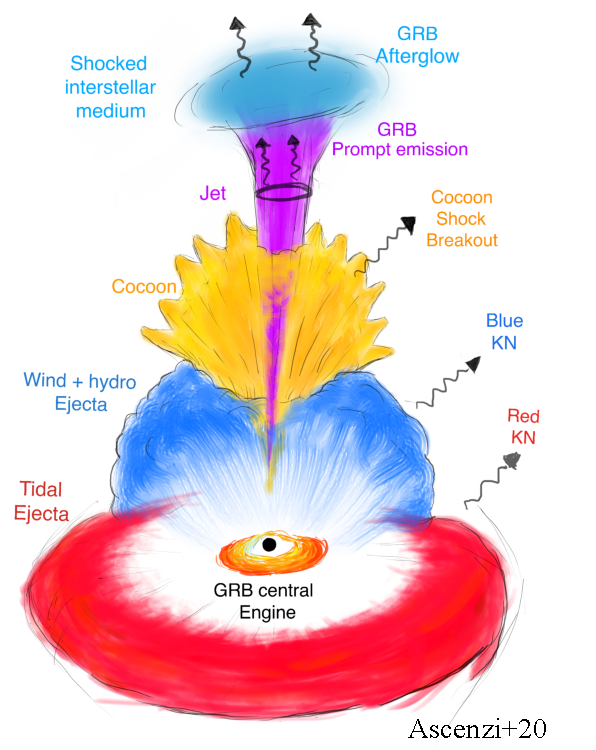
\includegraphics[height=7.0cm]{figures/Ascenzi20_EjectaEMPicture.pdf}
                    
                    %\small{\textbf{Artist depiction of ejecta$^\text{\citep{Ascenzi:2020xqi}}$}}
            }};
        }
    \end{tikzpicture}
\end{frame}

%                    \begin{itemize}
%    \item Electrons, moving in a magnetic field emit "curavature" radiation. 
%    \item Relativistic (non-relativistic) electrons emit synchrotron (cyclotron)
%    \item Both limits can be treated analytically. Trnasion -- cannot. 
%    \item Cyclotron emission is common in solar flare modelling. 
%    %                        \item If magnetic fields are very strong, cyclotron harmonics develope fine structure. 
%    \item (i) Neglecting quantum effects. 
%    \item Cyclotron radiation: observer sees specturm composed of delta factions at $\omega_0$; % orbital frequency.
%    \item As electron speeds up: observer sees additional Fourier components (harmonics), $\omega_0 \propto \gamma_e^{-1}$, emission becomes more beamed in the direction of motion. 
%    \item For a realtivistc electron: spectrim is a close series of delta functions (continous) 
%    up to $\omega \sim \omega_{b}\gamma_e^2$ with universal shape. % cyclotron frequency $omega_b = eB/m_ec$
%\end{itemize}

% =============================================================================================
\section{GRB afterglow}
\begin{frame}{}  %% ---------- Intro/motivation 
    \begin{tikzpicture}[overlay,remember picture]
        \uncover<1->{ % <-> |
            \node (t1) [anchor=center,scale=1,opacity=1] at ([shift={(-3.2cm,-0.5cm)}]current page.center){
                \parbox{0.65\textwidth}{
                    \textbf{Main Features}:
                    \begin{itemize}
                        \item Short \& Long
                        %
                        \item Three main stages: thermal/photosphere, prompt, \textbf{afterglow}
                         ( flares, shallow rise, rebrightening$(^*)$ )
                        %
                        \item Display plateus, flares, rebrightening($^*$)
                        %
                        \item Afterglow: synchrotron emission from (and forward shock). 
                        %
                    \end{itemize}
                    
                    \textbf{Observations of afterglow describe:}: 
                    \begin{itemize}
                        \item $F_{\nu;p}\propto E_{\rm iso} n_{\rm ISM}^{(p+1)/4}\theta_{\rm obs}^{-2p}\varepsilon_e^{p-1}\varepsilon_B^{(p+1)/4}D_{L}\nu^{(1-p)/2}$
                        \item $t_p\propto E_{\rm iso}^{1/3}n_{\rm ISM}^{-1/3}\theta_{\rm obs}^2$
                        \item Jet composition (Baryonic vs Poyniting flux)
                        \item Late-time engine activity 
                    \end{itemize}
%                    Difeverse afterglow-scape: plateus, flares, shallow rise, rebrightening(?)
%                    $\rightarrow$ central enigine activity. 
%                    (Reverse shock probes jet properties Poynting flux/baryon dominated)
%                    %
%                    Example: GRB170817A, sGRB from BNS merger. 
%                    Afterglow modelling $\rightarrow$ contraints on inclanation angle. 
            }};
            
        }
        
        %        \uncover<1->{ % <-> |
            %            \node (t1) [anchor=center,scale=1,opacity=1] at ([shift={(-3.5cm,-2.4cm)}]current page.center){
                %                \parbox{0.6\textwidth}{
                    %                    \begin{itemize}
                        %                        \item Kilonova: decay of $r$-process elements. Days-Weeks.
                        %                        \item Afterglow: synchrotron emission from shocked ISM. Weeks-Years. 
                        %                    \end{itemize}
                    %            }};
            %        }
        
        \uncover<1-1>{ % <-> |
            \node (img1) [anchor=center,scale=1,opacity=1] at ([shift={(4.5cm,1.4cm)}]current page.center){
                \parbox{0.5\textwidth}{
                    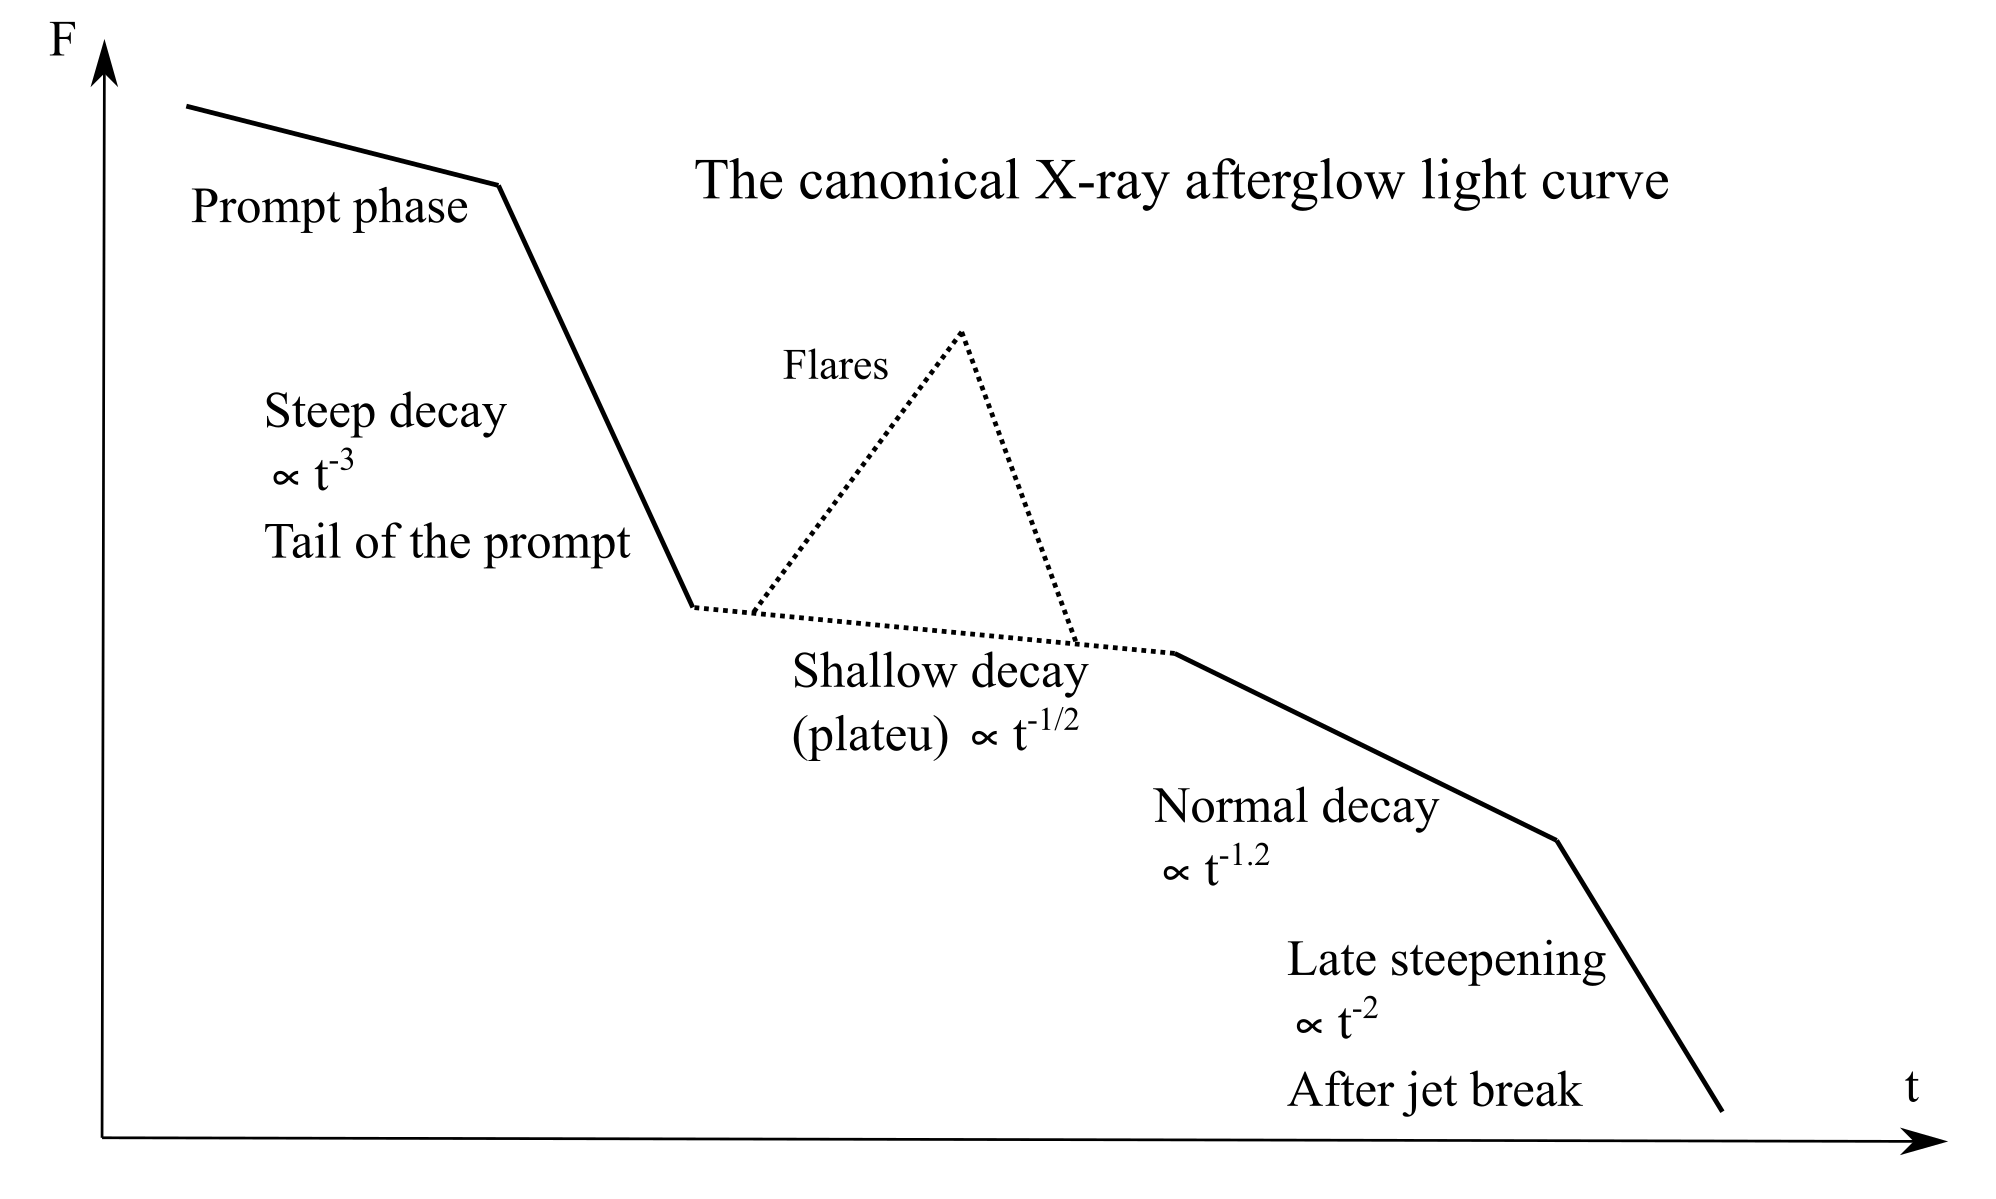
\includegraphics[height=4.2cm]{figures/grb_xray_canonic.png}
                    
                    %\small{\textbf{Artist depiction of ejecta$^\text{\citep{Ascenzi:2020xqi}}$}}
            }};
        }
        \uncover<1-1>{ % <-> |
            \node (img1) [anchor=center,scale=1,opacity=1] at ([shift={(5.0cm,-2.4cm)}]current page.center){
                \parbox{0.5\textwidth}{
                    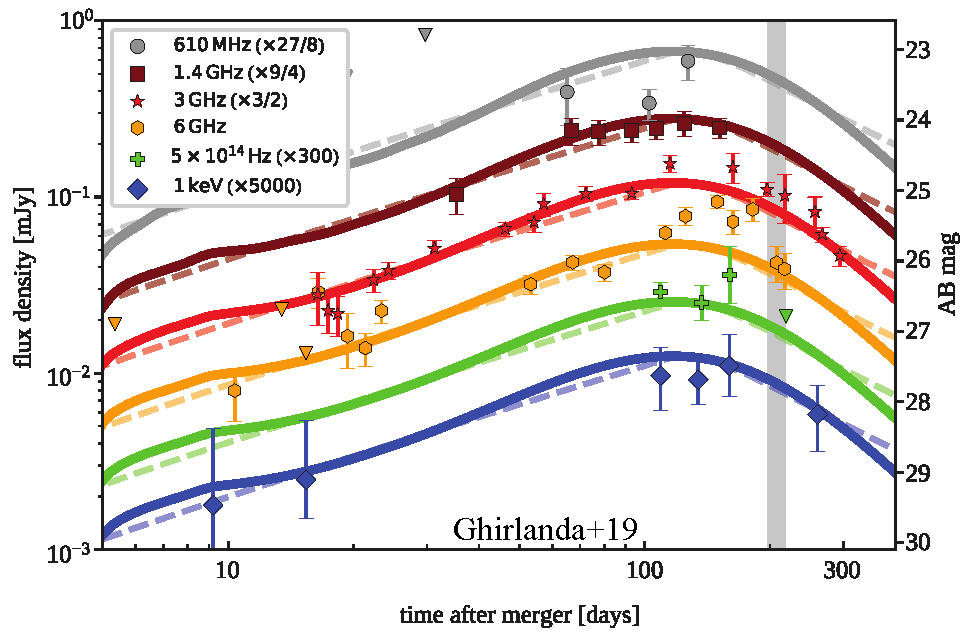
\includegraphics[height=3.8cm]{figures/Ghirlanda19_GRB170817A.pdf}
                    
                    %\small{\textbf{Artist depiction of ejecta$^\text{\citep{Ascenzi:2020xqi}}$}}
            }};
        }
    \end{tikzpicture}
\end{frame}


% =============================================================================================
\section{kN afterglows}
\begin{frame}{}  %% ---------- Intro/motivation 
    \begin{tikzpicture}[overlay,remember picture]
        \uncover<1->{ % <-> |
            \node (t1) [anchor=center,scale=1,opacity=1] at ([shift={(-3.1cm,-0.5cm)}]current page.center){
                \parbox{0.68\textwidth}{
                    \textbf{Main Features}:
                    \begin{itemize}
                        \item Synchrotron emission from mildly relativistic ejecta
                        (phenomenologically similar to GRB afterglow and SNe remnants)
                        %
                        \item Expected in sGRBs but have not observed$(^*)$
                        %
                        \item Complex ejecta structure/geometry $\rightarrow$ non-trivial EM signature
                        %
                    \end{itemize}
                    
                    \textbf{Information can be gained}: 
                    \begin{itemize}
                        \item $F_{\nu,p}\propto E n^{(p+1)/4}\beta^{(5p-7)/2}\varepsilon_e^{p-1}\varepsilon_B^{(p+1)/4}D_L^{-2}\nu^{(-p-1)/2}$
                        \item $t_{p}\propto E^{1/3} n_{\rm ISM}^{-1/3} \beta^{-5/3}$
                        %
                        \item Observed on a timescale of years.
                        %
                        \item Trace the properties of the fastest ejecta
                        %
                    \end{itemize}
            }};
        }
        %        
        %        \uncover<1->{ % <-> |
            %            \node (t1) [anchor=center,scale=1,opacity=1] at ([shift={(0.0cm,-3.8cm)}]current page.center){
                %                \parbox{1.1\textwidth}{
                    %                    \red{Questions}: remnant's lifetime; ejecta properties; \rproc{} cites
                    %            }};
            %        }
%        \uncover<1-1>{ % <-> |
%            \node (img1) [anchor=center,scale=1,opacity=1] at ([shift={(5.0cm,1.8cm)}]current page.center){
%                \parbox{0.5\textwidth}{
%                    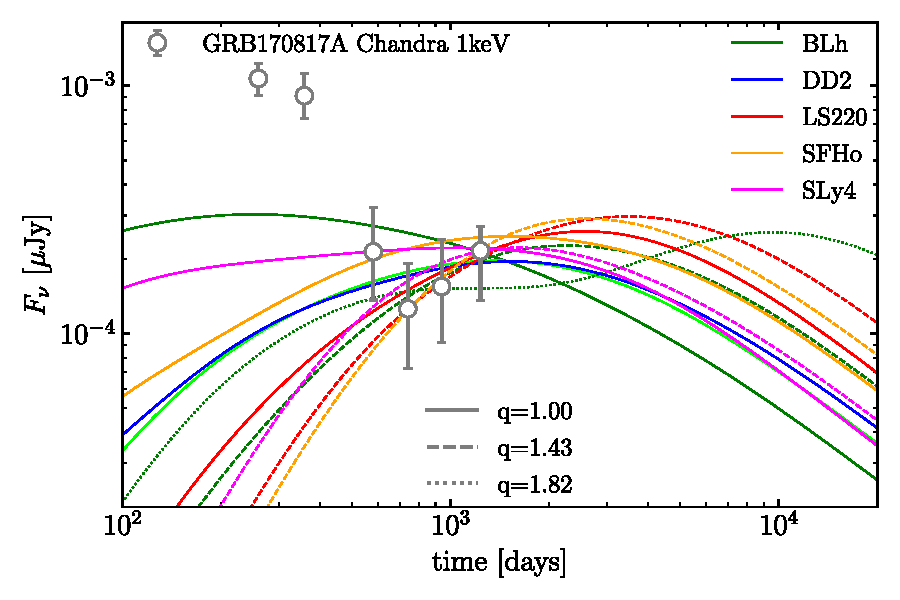
\includegraphics[height=3.8cm]{figures/best_xray_obs_representative_all_eos.pdf}
%                    
%                    %\small{\textbf{Artist depiction of ejecta$^\text{\citep{Ascenzi:2020xqi}}$}}
%            }};
%        }
        \uncover<1-1>{ % <-> |
            \node (img1) [anchor=center,scale=1,opacity=1] at ([shift={(5.2cm,-4.2cm)}]current page.center){
                \parbox{0.5\textwidth}{
                    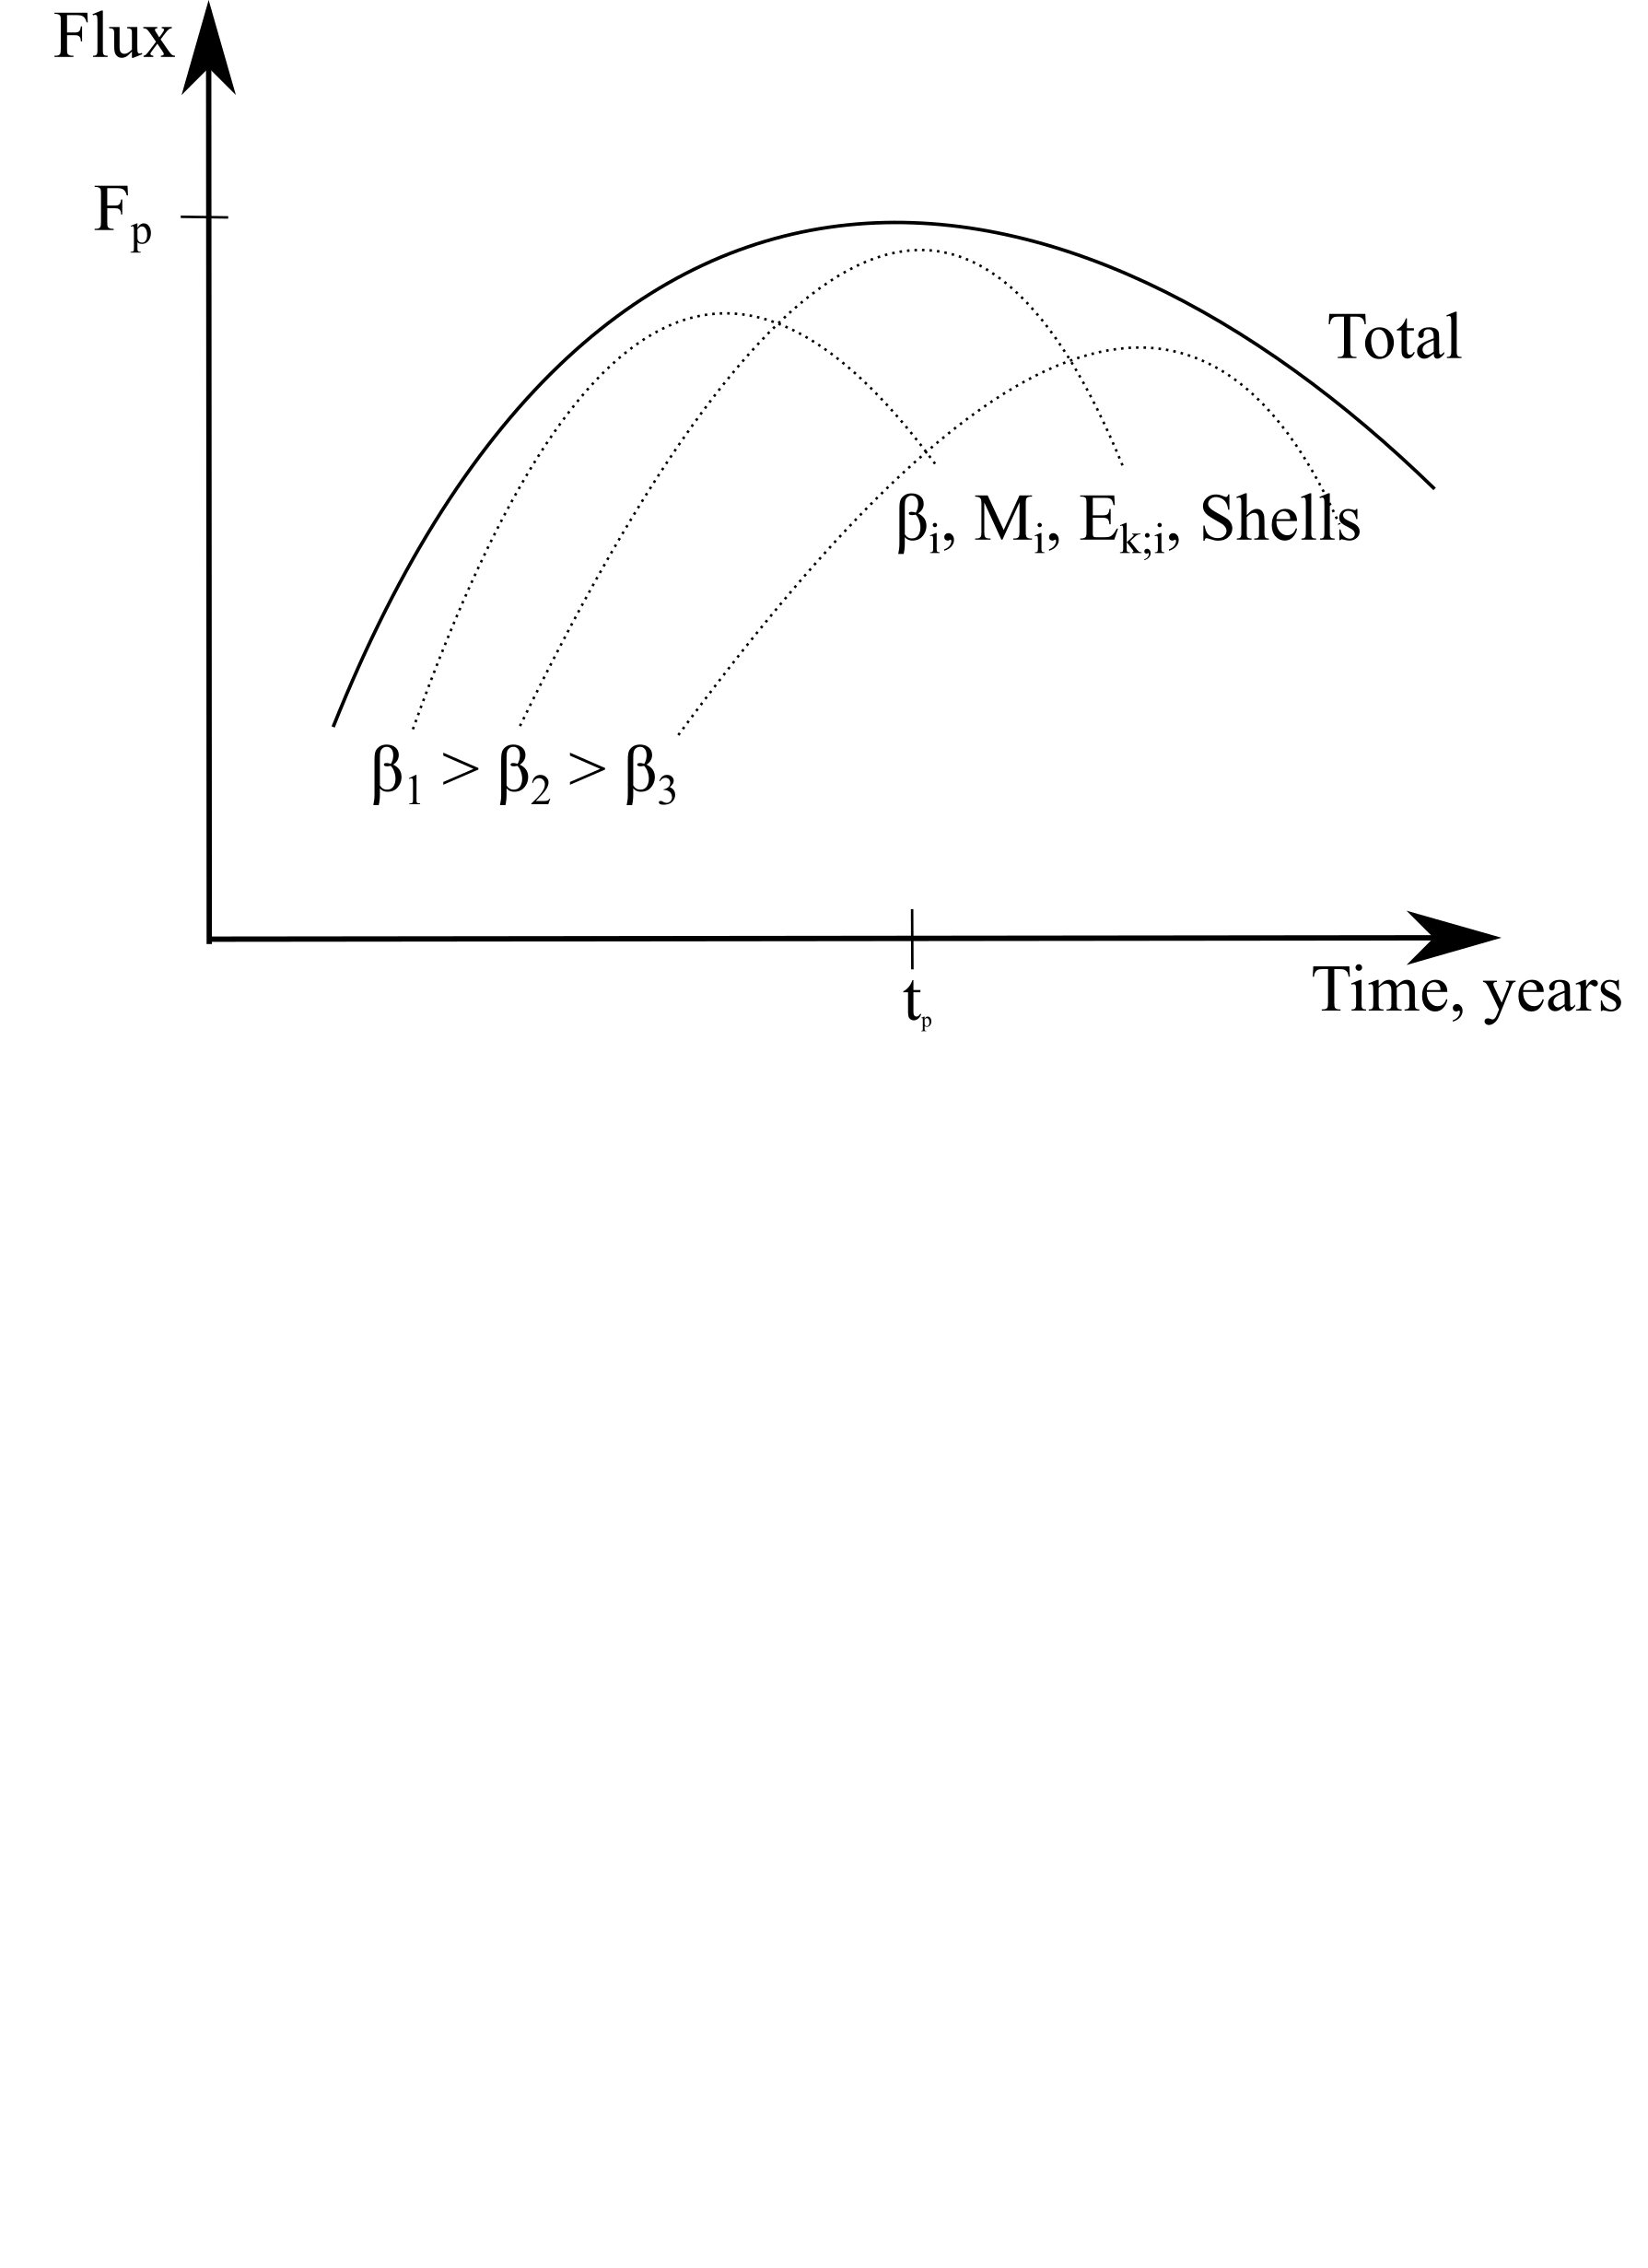
\includegraphics[height=8.6cm]{figures/afterglow_example.png}
                
                %\small{\textbf{Artist depiction of ejecta$^\text{\citep{Ascenzi:2020xqi}}$}}
            }};
        }
    \end{tikzpicture}
\end{frame}


% =============================================================================================

\section{Geometry}
\begin{frame}{}  %% ---------- Intro/motivation 
    \begin{tikzpicture}[overlay,remember picture]
        \uncover<1->{ % <-> |
            \node (t1) [anchor=center,scale=1,opacity=1] at ([shift={(-3.5cm,-0.5cm)}]current page.center){
                \parbox{0.6\textwidth}{
                    \textbf{Goal: combine structured GRB and kilonova afterglows}. \\
                    \textbf{Key features}:
                    \begin{itemize}
                        \item lateral structure \& lateral spreading of GRB ejecta
                        \item lateral \& velocity structure of kilonova ejecta
                        \item GRB jet evacuates ISM in front of ejecta
                        \item thermal electrons contribute to synchrotron emission from kilonova ejecta
                    \end{itemize}
            }};
            
        }
        %        
        %        \uncover<1->{ % <-> |
            %            \node (t1) [anchor=center,scale=1,opacity=1] at ([shift={(0.0cm,-3.8cm)}]current page.center){
                %                \parbox{1.1\textwidth}{
                    %                    \red{Questions}: remnant's lifetime; ejecta properties; \rproc{} cites
                    %            }};
            %        }
        \uncover<1-1>{ % <-> |
            \node (img1) [anchor=center,scale=1,opacity=1] at ([shift={(4.5cm,-0.5cm)}]current page.center){
                \parbox{0.5\textwidth}{
                    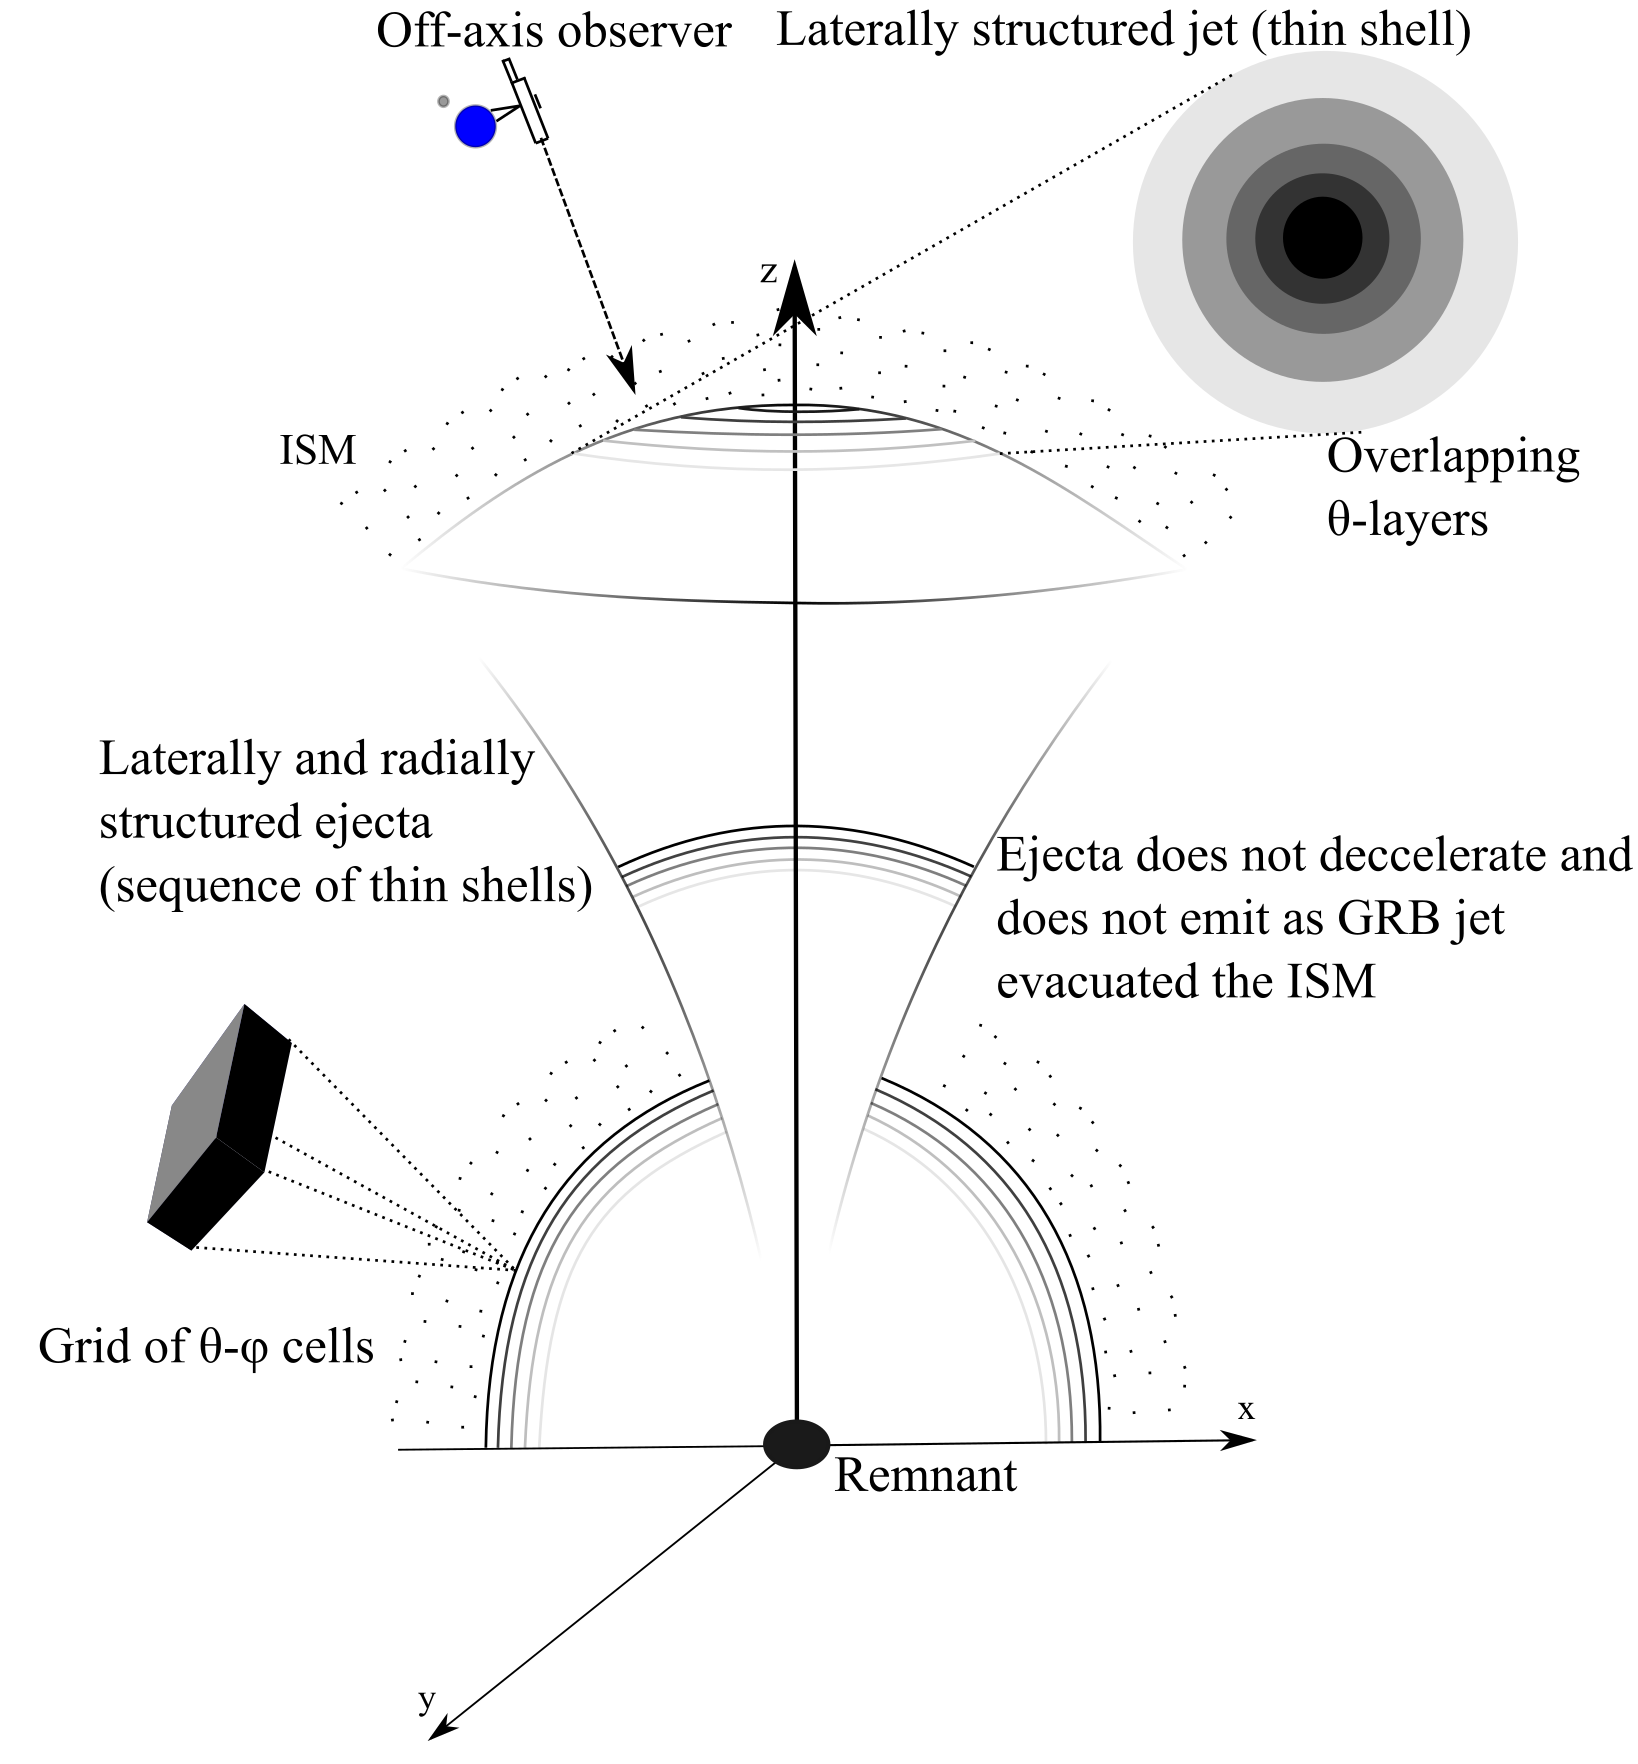
\includegraphics[height=7.2cm]{figures/structure.png}
                    
                    %\small{\textbf{Artist depiction of ejecta$^\text{\citep{Ascenzi:2020xqi}}$}}
            }};
        }
    \end{tikzpicture}
\end{frame}



% =============================================================================================

\section{Phsyics}
\subsection{Dynamics}
\begin{frame}{}  %% ---------- Intro/motivation 
    \begin{tikzpicture}[overlay,remember picture]
        \uncover<1->{ % <-> |
            \node (t1) [anchor=center,scale=1,opacity=1] at ([shift={(-3.5cm,-0.5cm)}]current page.center){
                \parbox{0.6\textwidth}{
                    Blast wave dynamics under ``thin-shell'' approximation. 
                    \begin{itemize}
                        \item jet/ejection duration is short (ejecta thickness is small)
                        \item $E_{\rm kin} \gg e_{\rm th}, p$
                        \item $4$ region system 
                    \end{itemize}
                    \begin{equation*}
                        E = \Gamma M_{0} c^2 + T^{00}V, \hspace{2mm}
                        T^{00} = (\epsilon' + P')\Gamma - P'
                    \end{equation*}
                    \begin{equation*}
                        P' = (4/3)(\Gamma^2-1)\rho c^2, \hspace{2mm}
                        \rho' = 4\Gamma\rho, \hspace{2mm}
                        \epsilon' = 4\Gamma\rho c^2
                    \end{equation*}
                    After $dt$, blast-wave speeps up $dm$ 
                    from ISM, and energy consiervation gives $d\Gamma$.
                    Separate presciption for spreading $d\theta/dt$. 
            }};
        }
        \uncover<1->{ % <-> |
            \node (t1) [anchor=center,scale=1,opacity=1] at ([shift={(4.2cm,-2.0cm)}]current page.center){
                \parbox{0.5\textwidth}{
                    Turbulent magnetic fields in the shock downstream \& first order Fermi acceleration
                    \begin{itemize}
                        \item Equipartition parameters $\varepsilon_e$, $\varepsilon_B$
                        \item first order Fermi acceleration of electrons
                        \item Non-thermal (thernal) electron population
                    \end{itemize}
            }};
        }
        \uncover<1-1>{ % <-> |
            \node (img1) [anchor=center,scale=1,opacity=1] at ([shift={(4.0cm,2.0cm)}]current page.center){
                \parbox{0.5\textwidth}{
                    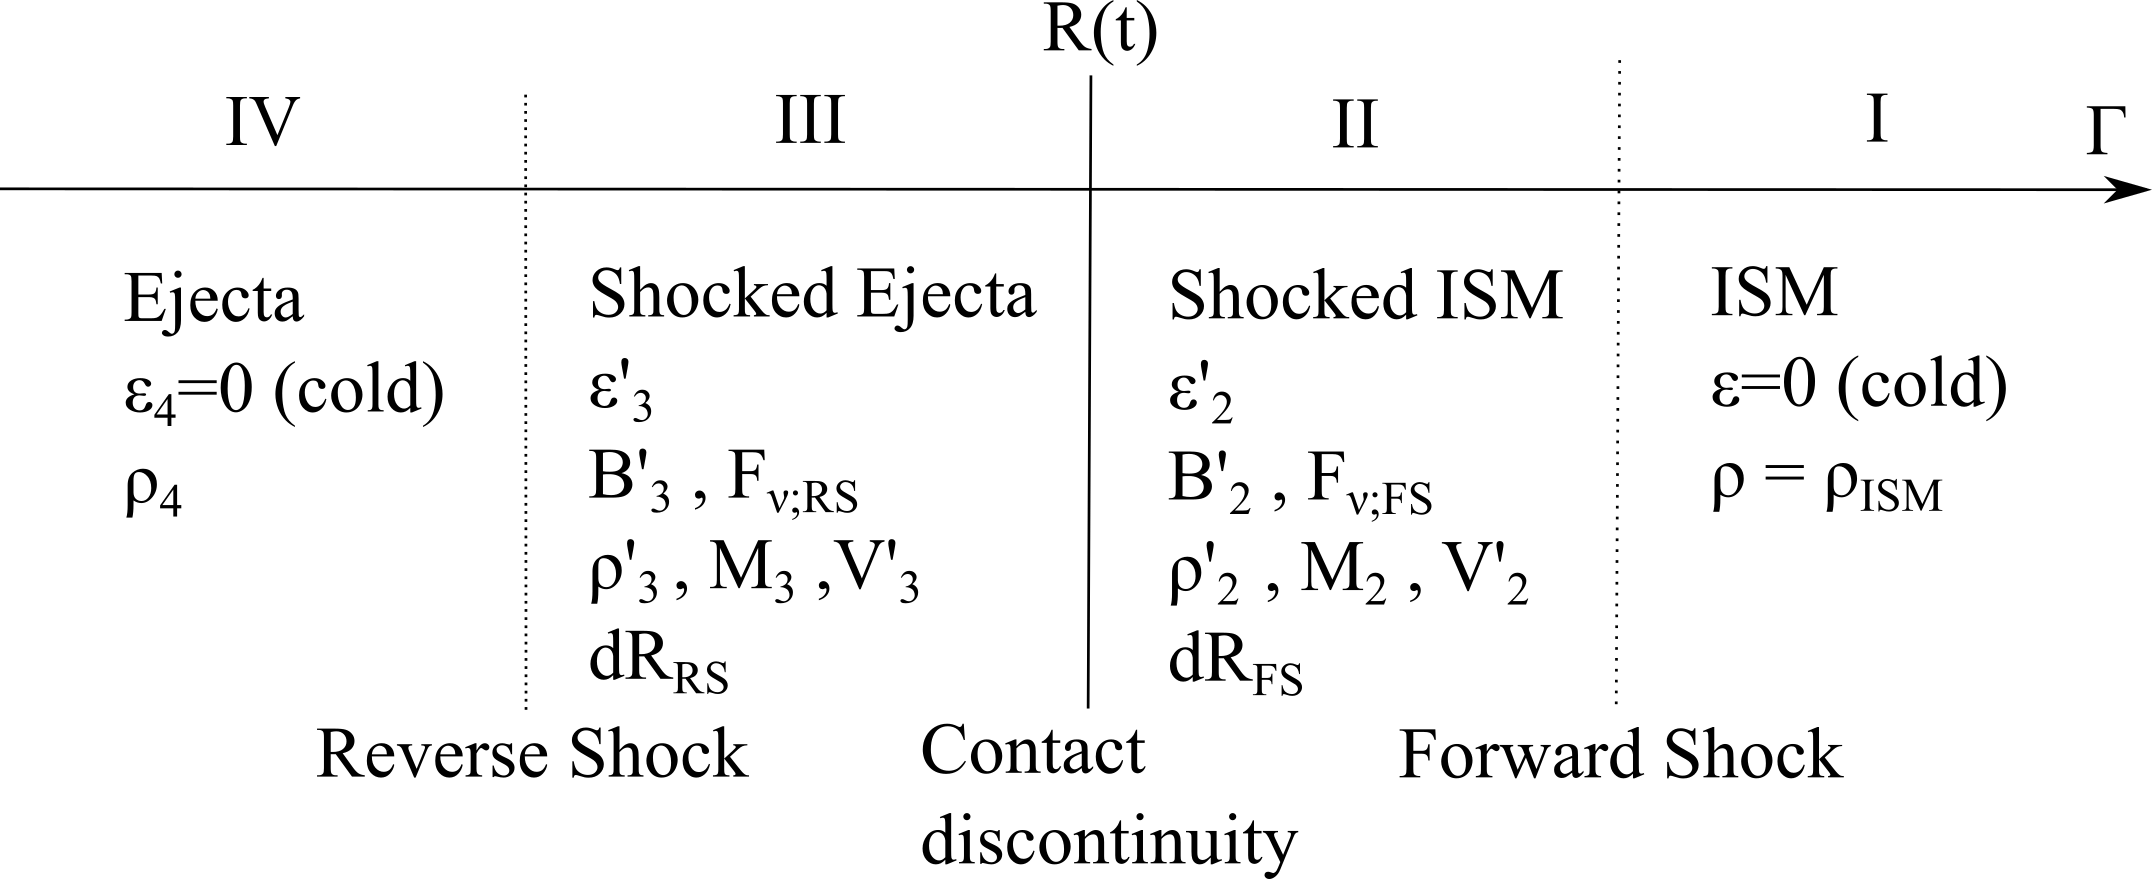
\includegraphics[height=3.0cm]{figures/blast_wave_struct.png}
            }};
        }
    \end{tikzpicture}
\end{frame}


% =============================================================================================

\subsection{Electron distribution in shock downstream}
\begin{frame}{}  %% ---------- Intro/motivation 
    \begin{tikzpicture}[overlay,remember picture]
        \uncover<1->{ % <-> |
            \node (t1) [anchor=center,scale=1,opacity=1] at ([shift={(-3.8cm,-0.2cm)}]current page.center){
                \parbox{0.5\textwidth}{
                    % power = energy/time/steradian/frequency
                    Fokker-Plank type equation:
%                    \begin{equation*}
%                        \frac{\partial}{\partial t}n_e(\gamma_e,t) = \frac{\partial}{\partial \gamma_e} \Bigg( -\frac{\sigma_T B^2}{6 \pi m_e c} \gamma_e^2 \Bigg) n_e(\gamma_e, t) + Q(\gamma)
%                    \end{equation*},
%                    where $Q(\gamma_e)\propto\gamma_e^{-p}$ with $\gamma_{m}\leq\gamma_e\leq\gamma_{\rm max}$ 
                    %
                    \begin{equation*}
                        \frac{\partial N(\gamma, t')}{\partial t'} = -\frac{\partial}{\partial \gamma}\Big[ \big( \dot{\gamma}_{\rm syn} + \dot{\gamma}_{\rm adi} N(\gamma, t') \big)  \Big] + Q(\gamma, t')
                    \end{equation*}
                    %
                    \begin{equation*}
                        \dot{\gamma}_{\rm syn} = - \frac{4}{3}\frac{\sigma_T c}{m_e c^2}\gamma^2, \hspace{3mm} \dot{\gamma}_{\rm adi} = -\frac{\gamma \beta_e^2}{3}\frac{d\ln V'}{dt'}, 
                    \end{equation*}
                    %
                    \begin{equation*}
                        Q(\gamma,t) = 
%                        \frac{dN_{\rm inj}}{dt d\gamma}=
                        \begin{cases}
                            Q_0(\gamma_m, t)\Big(\frac{\gamma}{\gamma_m}\Big)^{-p} & \gamma\in(\gamma_m,\gamma_M), \\
                            0 & \text{elswhere}.
                        \end{cases}
                    \end{equation*}
                    %
                    Steady state solution $\partial/\partial t' = 0$ and $\dot{\gamma}_{\rm adi} = 0$.
                    Cooling $\gamma_c = 6\pi m_e c / ( \sigma_T B^2 t )$.
                    
                    Electron cooling modifies distribution
                }};
            }
        \uncover<1->{ % <-> |
            \node (t1) [anchor=center,scale=1,opacity=1] at ([shift={(4.5cm,-0.5cm)}]current page.center){
                \parbox{0.45\textwidth}{
                    %
%                    \begin{equation*}
%                        \gamma_c = \frac{6\pi m_e c}{\sigma_T B^2 t}, 
%                    \end{equation*}
                    Electrons $\gamma > \gamma_c$ occupy $(\gamma/\gamma_c)^{-1}\ll 1$ fractional depth. 
                    Effective line-of-sight electron distribution
                    \begin{equation*}
                        \Big\langle \frac{\partial N}{\partial \gamma} \Big\rangle \propto  \frac{\partial N}{\partial \gamma}  \min \Big( 1, \frac{\gamma_c}{\gamma} \Big)
                    \end{equation*}
                    %
                    \begin{equation*}
                        \Big\langle \frac{\partial N}{\partial \gamma} \Big\rangle_{\rm fc} \propto
                        \begin{cases}
                            \gamma^{-p} & \gamma_m < \gamma < \gamma_c; \\
                            \gamma^{-p-1} & \gamma > \gamma_c
                        \end{cases}
                    \end{equation*}
                    %
                    \begin{equation*}
                        \Big\langle \frac{\partial N}{\partial \gamma} \Big\rangle_{\rm sc} \propto
                        \begin{cases}
                            \gamma^2 & \gamma_c < \gamma < \gamma_m; \\
                            \gamma^{-p-1} & \gamma > \gamma_m
                        \end{cases}
                    \end{equation*}
                    %
                    Afterglow spectrum is defined by $\gamma_m$ and $\gamma_c$
            }};
        }
        
    \end{tikzpicture}
\end{frame}

% =============================================================================================

\subsection{Cyclosynchrotron emission}
\begin{frame}{}  %% ---------- Intro/motivation 
    \begin{tikzpicture}[overlay,remember picture]
        \uncover<1->{ % <-> |
            \node (t1) [anchor=center,scale=1,opacity=1] at ([shift={(-0.0cm,-0.2cm)}]current page.center){
                \parbox{1.1\textwidth}{
                    % power = energy/time/steradian/frequency
                    \begin{equation*}
                        \boldsymbol{\eta}(\boldsymbol{\beta},\theta)d\omega = \frac{e^2 \omega^2}{2 \pi c}\Bigg[ \sum_{m=1}^{\infty} \Bigg( \frac{\cos\theta - \beta_{||}}{\sin \theta} \Bigg)^2 J_m^2(x) + \beta_{\perp}^2 J_m^{'2}(x) \Bigg]\delta(y) d\omega
                    \end{equation*}
                    where $x = (\omega/\omega_0)\beta_{\perp}\sin\theta$
                    $y=m\omega_0 - \omega(1 - \beta_{||}\cos\theta)$,
                    $\delta(y)$ is the delta function $J_m(x)$ is the Bessel function, 
                    $\beta_{||} = \beta\cos\theta_p$, $\beta_{\perp}=\beta\sin\theta_p$, 
                    with $\theta_p=\angle(\boldsymbol{\beta},\boldsymbol{B})$.
                    \begin{itemize}
                        \item Cyclotron, $m\beta \ll 1$: Expand $J(x)$ to lowest $x$, for successive harminics. 
                        \item Synchrotron $\gamma_e \gg 1$ : $J(x)$ approximated by modified Bessel function
                    \end{itemize}
                    \begin{equation*}
                        \frac{dE}{d\omega} = \frac{\sqrt{3}e^3 B \sin\theta_p}{2 \pi m_e c^2}
                        \frac{\omega}{\omega_c}\int_{\omega/\omega_c}^{\infty}F_{5/3}(\xi)d\xi,
                    \end{equation*}
                    where $\omega_c = (3/2) \gamma^2 \omega_b \sin \theta_p$
                    \begin{equation*}
                        L_{\omega} = 
%                        \frac{dE}{d\omega}=
                        2\pi\int_0^1 
%                        d\beta n(\beta) 
                        \frac{\partial N}{\partial \gamma_e} d\gamma_e
                        \int_0^1 d(\cos\theta_p) \int_{-1}^{1}d(\cos\theta)\boldsymbol{\eta}_{\boldsymbol{\beta},\theta}.
                    \end{equation*}
            }};
        }
        %        
        %        \uncover<1->{ % <-> |
            %            \node (t1) [anchor=center,scale=1,opacity=1] at ([shift={(0.0cm,-3.8cm)}]current page.center){
                %                \parbox{1.1\textwidth}{
                    %                    \red{Questions}: remnant's lifetime; ejecta properties; \rproc{} cites
                    %            }};
            %        }
        
    \end{tikzpicture}
\end{frame}

% =============================================================================================

\subsection{Synchrotron spectrum from non-thermal electrons}
\begin{frame}{}  %% ---------- Intro/motivation 
    \begin{tikzpicture}[overlay,remember picture]
        \uncover<1->{ % <-> |
            \node (t1) [anchor=center,scale=1,opacity=1] at ([shift={(0.8cm,2.2cm)}]current page.center){
                \parbox{1.0\textwidth}{
                    \begin{itemize}
                        \item (i) low-energy tail $\nu < \min(\nu_m, \nu_c)$,
                        \item (ii) power-law segment $\nu\in(\nu_m,\nu_c)$
                        \item (iii) exponential cut-off $\nu>\max(\nu_m,\nu_c)$
                    \end{itemize}
            }};
        }
        \uncover<1->{ % <-> |
            \node (img1) [anchor=center,scale=1,opacity=1] at ([shift={(-0.8cm,-1.5cm)}]current page.center){
                \parbox{1.0\textwidth}{
                    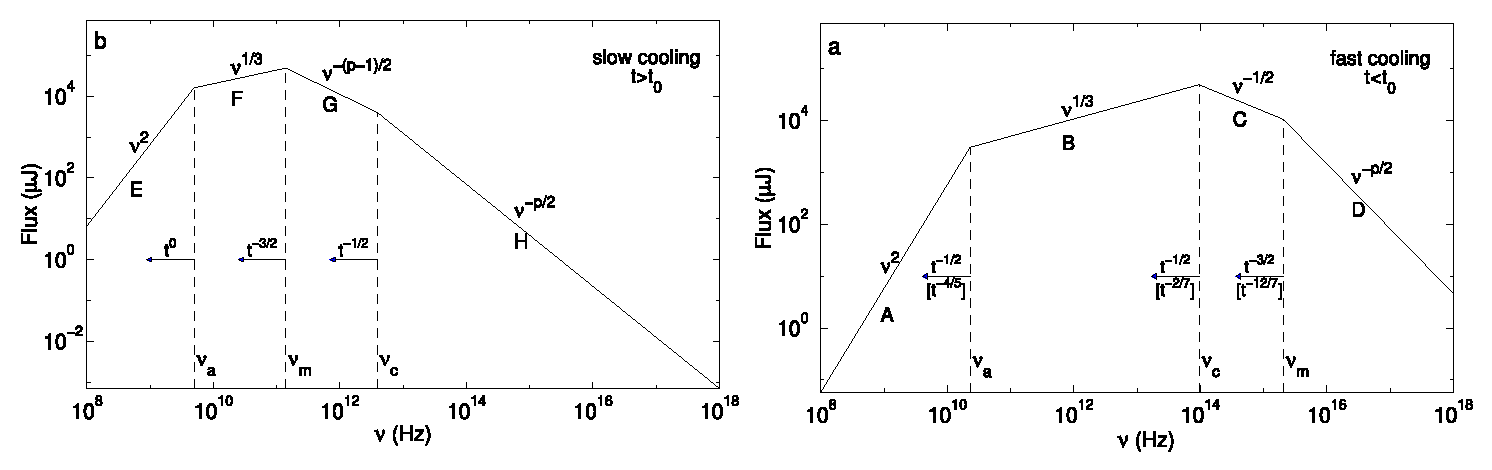
\includegraphics[height=5cm]{figures/sari97_flat.pdf}
            }};
        }
    \end{tikzpicture}
\end{frame}



% =============================================================================================

\section{Preliminary Results}
\subsection{Modelling sGRB afterglow (GRB170817A)}
\begin{frame}{}  %% ---------- Intro/motivation 
    \begin{tikzpicture}[overlay,remember picture]
         \uncover<1->{ % <-> |
            \node (t1) [anchor=center,scale=1,opacity=1] at ([shift={(-3.0cm,2.5cm)}]current page.center){
                \parbox{0.7\textwidth}{
                    \begin{itemize}
                        \item Gaussian jet $E(\theta) \propto e^{(\theta/\theta_c)^2}$
                        \item Off-axis $\theta_{\rm obs} > \theta_c$
                        \item Relativistic core, $\Gamma_c \sim 10^2$; low ISM density.
                    \end{itemize}
            }};
        }
        \uncover<1->{ % <-> |
            \node (img1) [anchor=center,scale=1,opacity=1] at ([shift={(1.cm,-1.35cm)}]current page.center){
                \parbox{1.0\textwidth}{
                    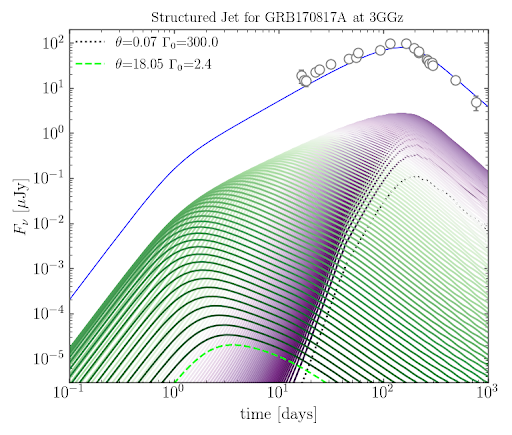
\includegraphics[height=6cm]{figures/grb170817fernandezPyBlastAfterglow.png}
            }};
        }
        \uncover<1->{ % <-> |
            \node (img1) [anchor=center,scale=1,opacity=1] at ([shift={(9.0cm,-0.5cm)}]current page.center){
                \parbox{1.0\textwidth}{
                    Flux centroid motion, $4.5\,$GGz; \\
                    Color is $I/I_{\rm max}$ %is shown with $I=0.01I_{\rm max}$ cut
                    
                    \movie[width=0.8\textwidth]{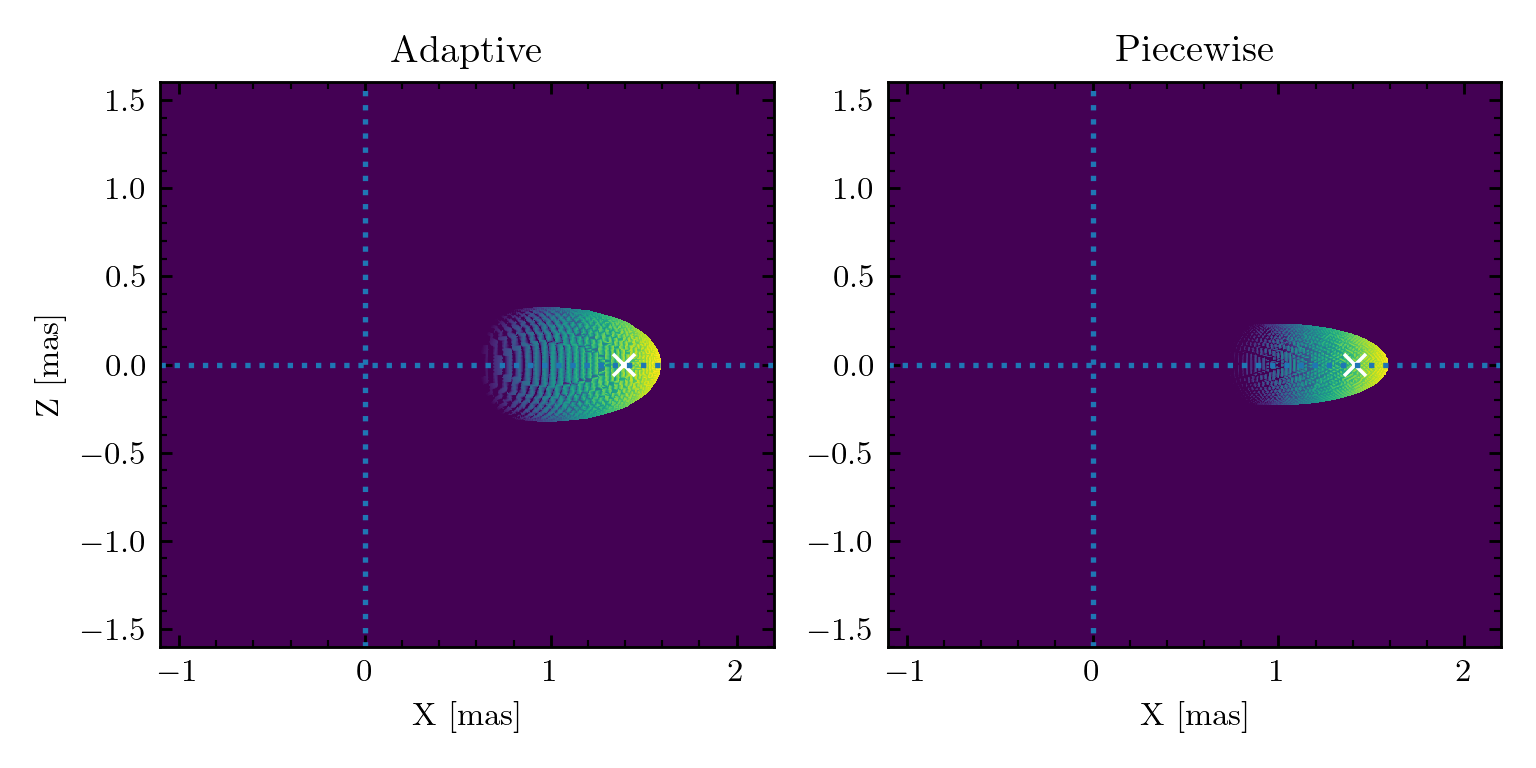
\includegraphics[width=0.8\textwidth]{figures/200.png}}{figures/out2.mp4}
            }};
        }
    \end{tikzpicture}
\end{frame}


% =============================================================================================

\subsection{Kilonova afterglow for NR ejecta profiles}
\begin{frame}{}  %% ---------- Intro/motivation 
    \begin{tikzpicture}[overlay,remember picture]
        \uncover<1->{ % <-> |
            \node (t1) [anchor=center,scale=1,opacity=1] at ([shift={(-3.1cm,-0.5cm)}]current page.center){
                \parbox{0.65\textwidth}{
                    \textbf{Main Features}:
                    \begin{itemize}
                        \item Set of NS BNS simulations targeted to \GW{}.
                        %
                        \item BNS model $(q,\tilde{\Lambda})$ $q=M_A/M_B$ is the mass ratio, $\tilde{\Lambda}$ tidal deformability parameter (Depends in EOS of NS)
                        %
                        \item Ejecta $M,\beta,E_k = f(q,\tilde{\Lambda})$
                        %
                    \end{itemize}
                    
                    \textbf{Information can be gained}: 
                    \begin{itemize}
                        \item New data for GRB170817A! Change in afterglow at $t_{\rm X}$
                        %
                        \item Compare light curves -- overall, agreement!
                        %
                        \item New avenue to constrain $q,\tilde{\Lambda}$!
                        %
                    \end{itemize}
            }};
        }
        %        
        %        \uncover<1->{ % <-> |
            %            \node (t1) [anchor=center,scale=1,opacity=1] at ([shift={(0.0cm,-3.8cm)}]current page.center){
                %                \parbox{1.1\textwidth}{
                    %                    \red{Questions}: remnant's lifetime; ejecta properties; \rproc{} cites
                    %            }};
            %        }
        \uncover<1-1>{ % <-> |
            \node (img1) [anchor=center,scale=1,opacity=1] at ([shift={(5.0cm,1.8cm)}]current page.center){
                \parbox{0.5\textwidth}{
                    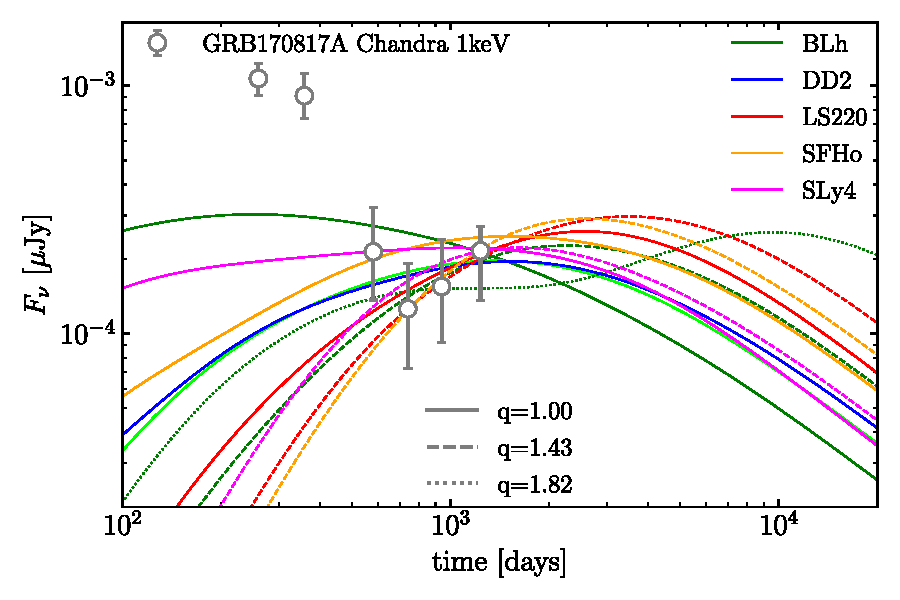
\includegraphics[height=3.8cm]{figures/best_xray_obs_representative_all_eos.pdf}
                    
                    %\small{\textbf{Artist depiction of ejecta$^\text{\citep{Ascenzi:2020xqi}}$}}
            }};
        }
        \uncover<1-1>{ % <-> |
            \node (img1) [anchor=center,scale=1,opacity=1] at ([shift={(5.2cm,-2.2cm)}]current page.center){
                \parbox{0.5\textwidth}{
                    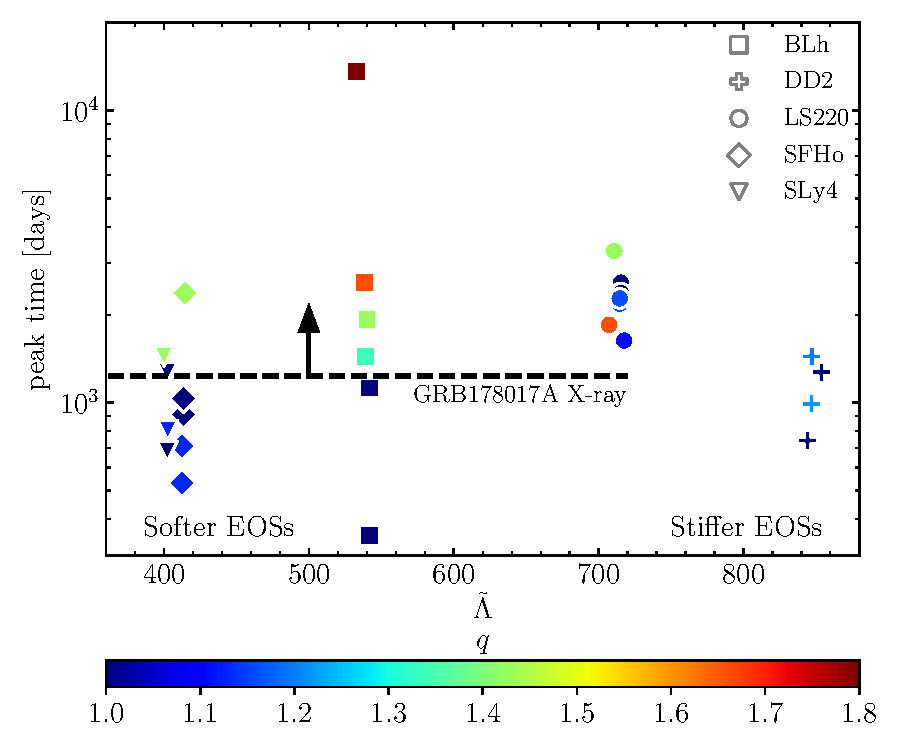
\includegraphics[height=4.2cm]{figures/scatter_lightcurve_tpeak_vs_lambda.pdf}
                    
                    %\small{\textbf{Artist depiction of ejecta$^\text{\citep{Ascenzi:2020xqi}}$}}
            }};
        }
    \end{tikzpicture}
\end{frame}

% =============================================================================================

\subsection{Thermal electrons in mildly relativistic shocks}
\begin{frame}{}  %% ---------- Intro/motivation 
    \begin{tikzpicture}[overlay,remember picture]
        \uncover<1->{ % <-> |
            \node (t1) [anchor=center,scale=1,opacity=1] at ([shift={(-3.0cm,2.2cm)}]current page.center){
                \parbox{0.5\textwidth}{
                    \begin{itemize}
                        \item ``Thermal spectrum'' (left)
                        \item ``Non-thermal spectrum'' (right)
                    \end{itemize}
                    $\beta_{\rm sh}=0.1$, $n_{\rm ISM}=10^4\,\ccm$, $t=200\,$d, $\delta=0.1$, $p=3$, $B=0.1\,$G, $\varepsilon_T=0.1$
            }};
        }
        \uncover<1->{ % <-> |
            \node (t1) [anchor=center,scale=1,opacity=1] at ([shift={(4.0cm,2.2cm)}]current page.center){
                \parbox{0.5\textwidth}{
                    \begin{eqnarray*}
                        \frac{\partial N}{\partial \gamma}\Big|_{\rm th} &= n_{e} \frac{ \gamma^2\sqrt{1-\gamma^{-2}} }{K_2(1/\Theta) \Theta} e^{-\gamma/\Theta}, \\
                        %                        \hspace{5mm}
                        \frac{\partial N}{\partial \gamma}\Big|_{\rm pl} &= n_e g(\Theta)\delta\frac{p-2}{3\Theta}\Big(\frac{\gamma}{3\Theta}\Big)^{-p}
                    \end{eqnarray*}
                    
                    
                    %                    Spectrum $3$ segments: 
                    %                    (i) $\nu < \nu_c$: low energy tail, $F_{\nu}\propto\nu^{1/3}$, 
                    %                    (ii) $\nu(\gamma) > \nu_c$ power law segment $F_{\nu}\propto\nu^{-1/2}$ 
                    %                    (iii) $\nu(\gamma)$and 
            }};
        }
        \uncover<1->{ % <-> |
            \node (img1) [anchor=center,scale=1,opacity=1] at ([shift={(2.cm,-1.5cm)}]current page.center){
                \parbox{1.0\textwidth}{
                    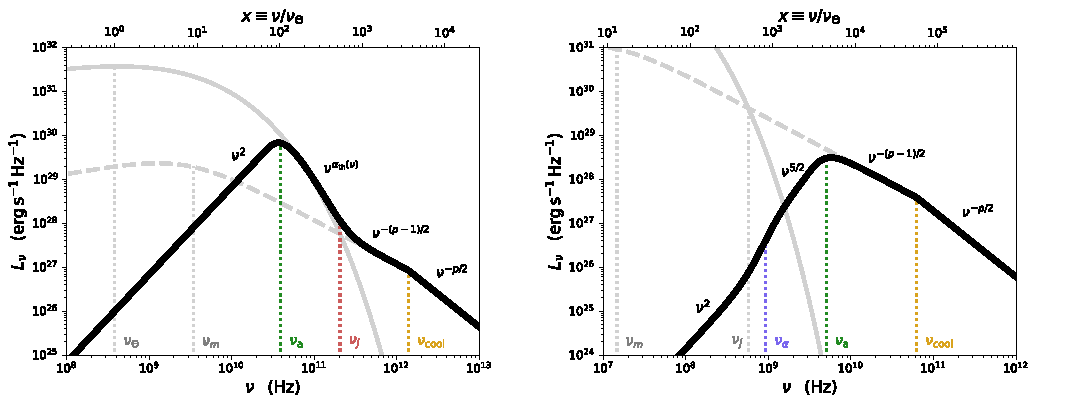
\includegraphics[height=5cm]{figures/Margalit21_thermalElectrons.pdf}
            }};
        }
    \end{tikzpicture}
\end{frame}
\begin{frame}{}  %% ---------- Intro/motivation 
    \begin{tikzpicture}[overlay,remember picture]
        \uncover<1->{ % <-> |
            \node (t1) [anchor=center,scale=1,opacity=1] at ([shift={(-5.0cm,1.2cm)}]current page.center){
                \parbox{0.4\textwidth}{
                    Comparison between two optically thin ight cruves:
                    \begin{itemize}
                        \item ``Thermal'' (blue)
                        \item ``Non-thermal'' (green)
                    \end{itemize}
                    Further investigations required! 
            }};
        }
        \uncover<1->{ % <-> |
            \node (img1) [anchor=center,scale=1,opacity=1] at ([shift={(6.cm,0.0cm)}]current page.center){
                \parbox{1.0\textwidth}{
                    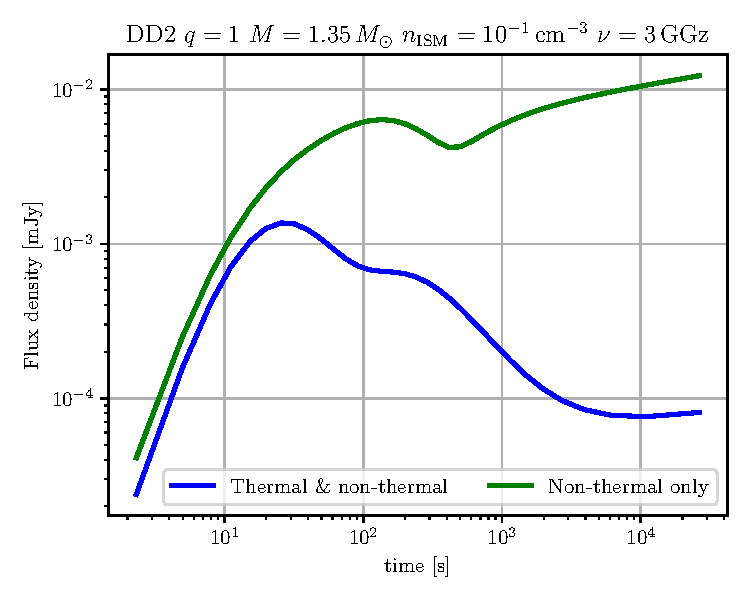
\includegraphics[height=7cm]{figures/test_thermal_electrons.pdf}
            }};
        }
    \end{tikzpicture}
\end{frame}

% =============================================================================================

\subsection{Extracting kilonova ejecta profile}
\begin{frame}{}  %% ---------- Intro/motivation 
    \begin{tikzpicture}[overlay,remember picture]
        \uncover<1->{ % <-> |
            \node (t1) [anchor=center,scale=1,opacity=1] at ([shift={(-3.0cm,2.5cm)}]current page.center){
                \parbox{0.7\textwidth}{
                    \begin{itemize}
                        \item $E_{\rm k} = f(\theta,\beta)$
                        \item $E_{\rm k;max}$ at $\theta\rightarrow0$ and $\beta\rightarrow0.2$.
                        \item $\log_{10}(E_k)=b_0 + (b_1 \theta) + (b_2 \beta) + (b_3 \theta^2) + (b_4 \theta \beta) + (b_5 \beta^{1/4})$
                    \end{itemize}
            }};
        }
        \uncover<1->{ % <-> |
            \node (img1) [anchor=center,scale=1,opacity=1] at ([shift={(2.2cm,-1.35cm)}]current page.center){
                \parbox{1.0\textwidth}{
                    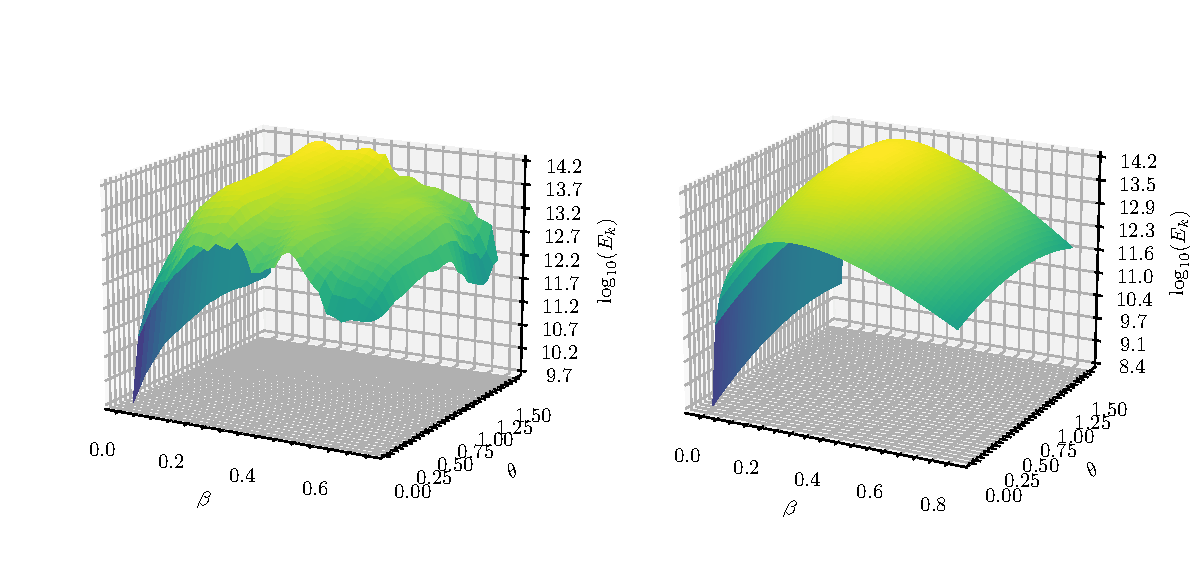
\includegraphics[height=6cm]{figures/fit_2d_ejecta.pdf}
            }};
        }
        \uncover<1->{ % <-> |
            \node (img1) [anchor=center,scale=1,opacity=1] at ([shift={(9cm,2cm)}]current page.center){
                \parbox{1.0\textwidth}{
                    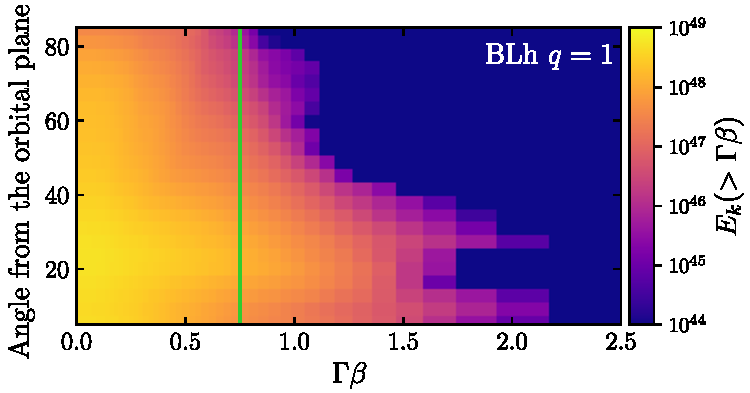
\includegraphics[height=3cm]{figures/kinetic_energy_struct_models_bottom_only.pdf}
            }};
        }
    \end{tikzpicture}
\end{frame}
%%% --------------------------------------------------------------
%%
%% T H E O R Y
%%
%% --------------------------------------------------------------



\section{Phsyics}
\subsection{Dynamics}
\begin{frame}{}  %% ---------- Intro/motivation 
    \begin{tikzpicture}[overlay,remember picture]
        \uncover<1->{ % <-> |
            \node (t1) [anchor=center,scale=1,opacity=1] at ([shift={(-3.5cm,-0.5cm)}]current page.center){
                \parbox{0.6\textwidth}{
                    Blast wave dynamics under ``thin-shell'' approximation. 
                    \begin{itemize}
                        \item jet/ejection duration is short (ejecta thickness is small)
                        \item $E_{\rm kin} \gg e_{\rm th}, P$
                        \item $4$ region system 
                    \end{itemize}
                    \begin{equation*}
                        E = \Gamma M_{0} c^2 + T^{00}V, \hspace{2mm}
                        T^{00} = (\epsilon' + P')\Gamma - P'
                    \end{equation*}
                    \begin{equation*}
                        P' = (4/3)(\Gamma^2-1)\rho c^2, \hspace{2mm}
                        \rho' = 4\Gamma\rho, \hspace{2mm}
                        \epsilon' = 4\Gamma\rho c^2
                    \end{equation*}
                    After $dt$, blast-wave sweeps up $dm$ 
                    from ISM, and energy conservation gives $d\Gamma$.
                    Separate inclusion of $d\theta/dt$. 
            }};
        }
        \uncover<1->{ % <-> |
            \node (t1) [anchor=center,scale=1,opacity=1] at ([shift={(4.2cm,-2.0cm)}]current page.center){
                \parbox{0.5\textwidth}{
                    \textbf{Shock downstream}: \\
                    \begin{itemize}
                        \item fluid compression;
                        \item magnetic field amplification ($\varepsilon_B$)
                        \item first order Fermi acceleration ($\varepsilon_e$)
                    \end{itemize}
            }};
        }
        \uncover<1-1>{ % <-> |
            \node (img1) [anchor=center,scale=1,opacity=1] at ([shift={(4.0cm,2.0cm)}]current page.center){
                \parbox{0.5\textwidth}{
                    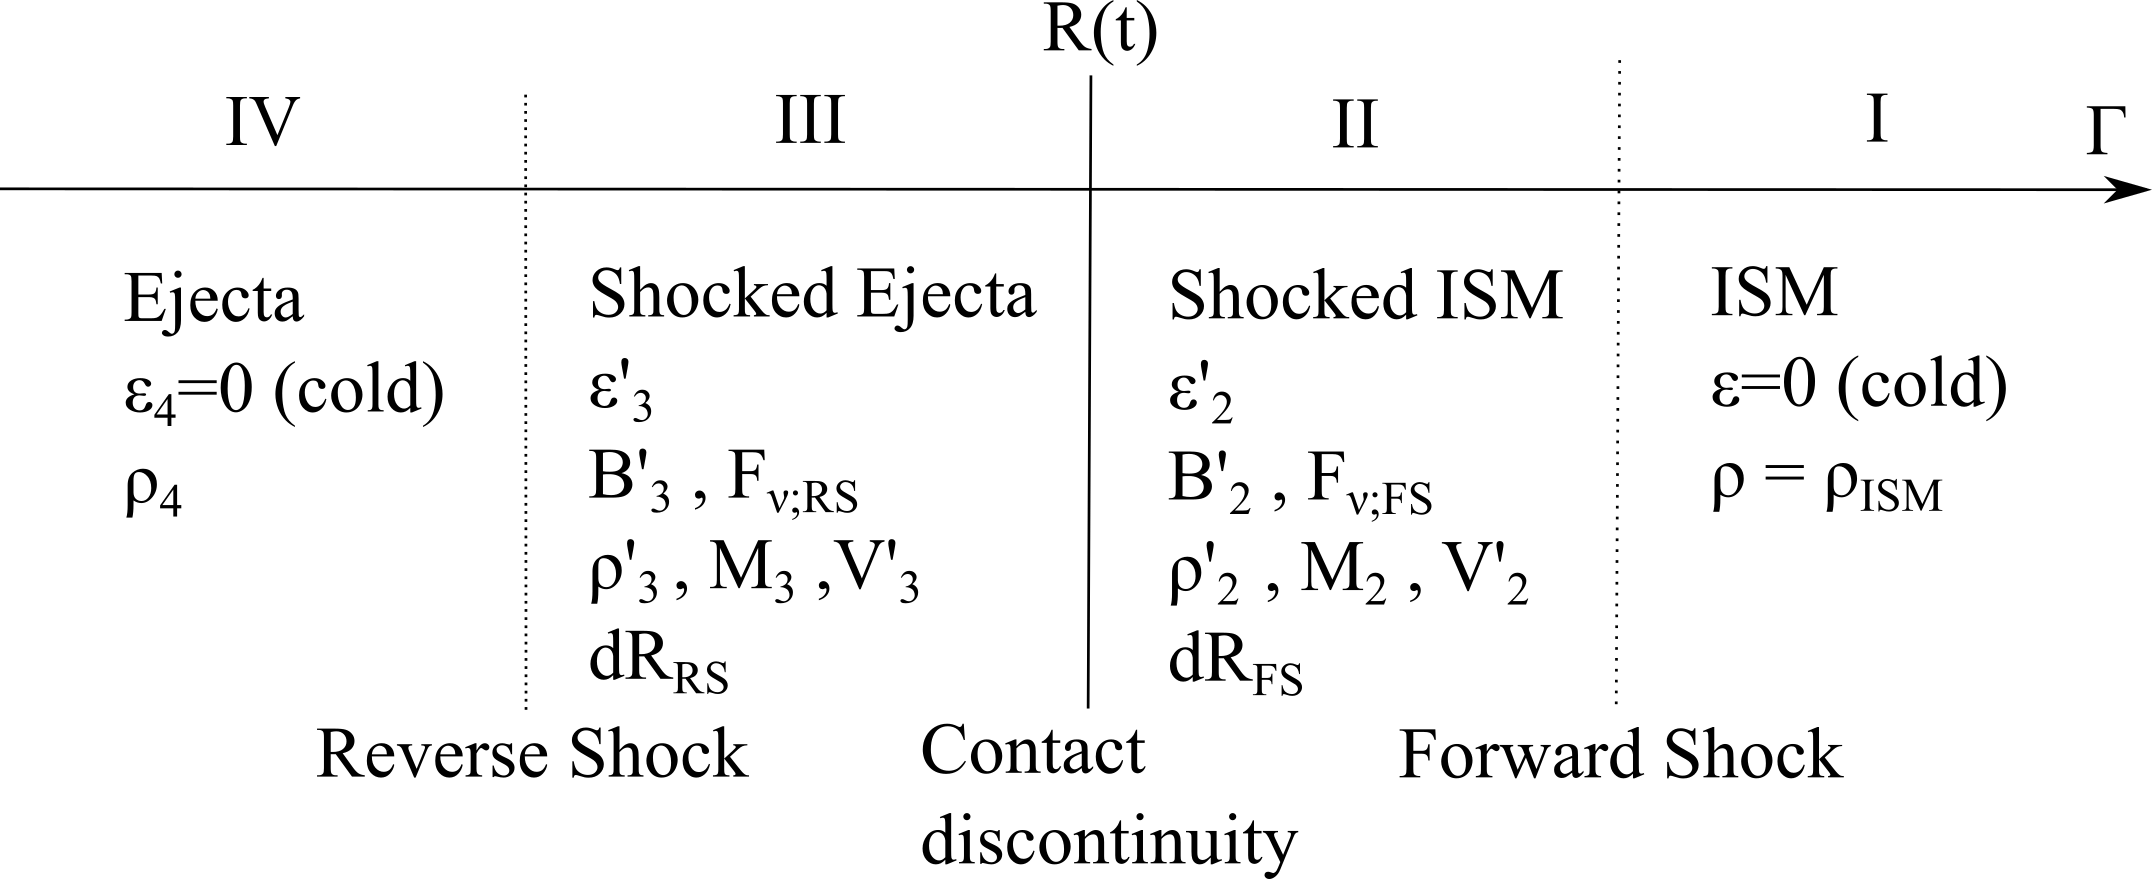
\includegraphics[height=3.0cm]{figures/blast_wave_struct.png}
            }};
        }
    \end{tikzpicture}
\end{frame}


% =============================================================================================

\subsection{Electron distribution in shock downstream}
\begin{frame}{}  %% ---------- Intro/motivation 
    \begin{tikzpicture}[overlay,remember picture]
        \uncover<1->{ % <-> |
            \node (t1) [anchor=center,scale=1,opacity=1] at ([shift={(-3.8cm,-0.2cm)}]current page.center){
                \parbox{0.5\textwidth}{
                    % power = energy/time/steradian/frequency
                    Fokker-Plank type equation:
                    %                    \begin{equation*}
                        %                        \frac{\partial}{\partial t}n_e(\gamma_e,t) = \frac{\partial}{\partial \gamma_e} \Bigg( -\frac{\sigma_T B^2}{6 \pi m_e c} \gamma_e^2 \Bigg) n_e(\gamma_e, t) + Q(\gamma)
                        %                    \end{equation*},
                    %                    where $Q(\gamma_e)\propto\gamma_e^{-p}$ with $\gamma_{m}\leq\gamma_e\leq\gamma_{\rm max}$ 
                    %
                    \begin{equation*}
                        \frac{\partial N(\gamma, t')}{\partial t'} = -\frac{\partial}{\partial \gamma}\Big[ \big( \dot{\gamma}_{\rm syn} + \dot{\gamma}_{\rm adi} N(\gamma, t') \big)  \Big] + Q(\gamma, t')
                    \end{equation*}
                    %
                    \begin{equation*}
                        \dot{\gamma}_{\rm syn} = - \frac{4}{3}\frac{\sigma_T c}{m_e c^2}\gamma^2, \hspace{3mm} \dot{\gamma}_{\rm adi} = -\frac{\gamma \beta_e^2}{3}\frac{d\ln V'}{dt'}, 
                    \end{equation*}
                    %
                    \begin{equation*}
                        Q(\gamma,t) = 
                        %                        \frac{dN_{\rm inj}}{dt d\gamma}=
                        \begin{cases}
                            \textcolor{red}{Q_0}(\gamma_m, t)\Big(\frac{\gamma}{\gamma_m}\Big)^{-p} & \gamma\in(\gamma_m,\gamma_M), \\
                            0 & \text{elswhere}.
                        \end{cases}
                    \end{equation*}
                    %
                    Is $Q_0 = f(B)$ -- YES! 
                    
                    Steady state solution $\partial/\partial t' = 0$ and $\dot{\gamma}_{\rm adi} = 0$.
                    Cooling $\gamma_c = 6\pi m_e c / ( \sigma_T B^2 t )$.
                    
                    Electron cooling modifies distribution
            }};
        }
        \uncover<1->{ % <-> |
            \node (t1) [anchor=center,scale=1,opacity=1] at ([shift={(4.5cm,-0.5cm)}]current page.center){
                \parbox{0.45\textwidth}{
                    %
                    %                    \begin{equation*}
                        %                        \gamma_c = \frac{6\pi m_e c}{\sigma_T B^2 t}, 
                        %                    \end{equation*}
                    Electrons $\gamma > \gamma_c$ occupy $(\gamma/\gamma_c)^{-1}\ll 1$ fractional depth. 
                    Effective line-of-sight electron distribution
                    \begin{equation*}
                        \Big\langle \frac{\partial N}{\partial \gamma} \Big\rangle \propto  \frac{\partial N}{\partial \gamma}  \min \Big( 1, \frac{\gamma_c}{\gamma} \Big)
                    \end{equation*}
                    %
                    \begin{equation*}
                        \Big\langle \frac{\partial N}{\partial \gamma} \Big\rangle_{\rm fc} \propto
                        \begin{cases}
                            \gamma^{-p} & \gamma_m < \gamma < \gamma_c; \\
                            \gamma^{-p-1} & \gamma > \gamma_c
                        \end{cases}
                    \end{equation*}
                    %
                    \begin{equation*}
                        \Big\langle \frac{\partial N}{\partial \gamma} \Big\rangle_{\rm sc} \propto
                        \begin{cases}
                            \gamma^2 & \gamma_c < \gamma < \gamma_m; \\
                            \gamma^{-p-1} & \gamma > \gamma_m
                        \end{cases}
                    \end{equation*}
                    %
                    Afterglow spectrum is defined by $\gamma_m$ and $\gamma_c$
            }};
        }
    \end{tikzpicture}
\end{frame}



% =============================================================================================

\subsection{Cyclosynchrotron emission}
\begin{frame}{}  %% ---------- Intro/motivation 
    \begin{tikzpicture}[overlay,remember picture]
        \uncover<1->{ % <-> |
            \node (t1) [anchor=center,scale=1,opacity=1] at ([shift={(-0.0cm,-0.2cm)}]current page.center){
                \parbox{1.1\textwidth}{
                    % power = energy/time/steradian/frequency
                    \begin{equation*}
                        \boldsymbol{\eta}(\boldsymbol{\beta},\theta)d\omega = \frac{e^2 \omega^2}{2 \pi c}\Bigg[ \sum_{m=1}^{\infty} \Bigg( \frac{\cos\theta - \beta_{||}}{\sin \theta} \Bigg)^2 J_m^2(x) + \beta_{\perp}^2 J_m^{'2}(x) \Bigg]\delta(y) d\omega
                    \end{equation*}
                    where $x = (\omega/\omega_0)\beta_{\perp}\sin\theta$
                    $y=m\omega_0 - \omega(1 - \beta_{||}\cos\theta)$,
                    $\delta(y)$ is the delta function $J_m(x)$ is the Bessel function, 
                    $\beta_{||} = \beta\cos\theta_p$, $\beta_{\perp}=\beta\sin\theta_p$, 
                    with $\theta_p=\angle(\boldsymbol{\beta},\boldsymbol{B})$.
                    \begin{itemize}
                        \item Cyclotron, $m\beta \ll 1$: Expand $J(x)$ to lowest $x$, for successive harminics. 
                        \item Synchrotron $\gamma_e \gg 1$ : $J(x)$ approximated by modified Bessel function
                    \end{itemize}
                    \begin{equation*}
                        \frac{dE}{d\omega} = \frac{\sqrt{3}e^3 B \sin\theta_p}{2 \pi m_e c^2}
                        \frac{\omega}{\omega_c}\int_{\omega/\omega_c}^{\infty}F_{5/3}(\xi)d\xi,
                    \end{equation*}
                    where $\omega_c = (3/2) \gamma^2 \omega_b \sin \theta_p$
                    \begin{equation*}
                        L_{\omega} = 
                        %                        \frac{dE}{d\omega}=
                        2\pi\int_0^1 
                        %                        d\beta n(\beta) 
                        \frac{\partial N}{\partial \gamma_e} d\gamma_e
                        \int_0^1 d(\cos\theta_p) \int_{-1}^{1}d(\cos\theta)\boldsymbol{\eta}_{\boldsymbol{\beta},\theta}.
                    \end{equation*}
            }};
        }
        %        
        %        \uncover<1->{ % <-> |
            %            \node (t1) [anchor=center,scale=1,opacity=1] at ([shift={(0.0cm,-3.8cm)}]current page.center){
                %                \parbox{1.1\textwidth}{
                    %                    \red{Questions}: remnant's lifetime; ejecta properties; \rproc{} cites
                    %            }};
            %        }
        
    \end{tikzpicture}
\end{frame}

% =============================================================================================

\subsection{Synchrotron spectrum from non-thermal electrons}
\begin{frame}{}  %% ---------- Intro/motivation 
    \begin{tikzpicture}[overlay,remember picture]
        \uncover<1->{ % <-> |
            \node (t1) [anchor=center,scale=1,opacity=1] at ([shift={(-4.0cm,2.2cm)}]current page.center){
                \parbox{0.55\textwidth}{
                    Consider
                    $dN/d\gamma_e\propto \gamma^{-p}$, with min. $\gamma_m$ and cool. $\gamma_c$. \\
                    Spectrum is determined by the location of $\nu_c = \gamma_c^2 \nu_g$, 
                    $\nu_g=q_e B / (2\pi m_e c)$ is a gyrofrequency. $F_{\nu}=N_e P_{\nu;\rm max}/4\pi D^2$  where $P_{\nu}\approx \Gamma B m_e c^2 \sigma_T / 3q_e$
            }};
        }
        \uncover<1->{ % <-> |
            \node (t1) [anchor=center,scale=1,opacity=1] at ([shift={(4.0cm,2.2cm)}]current page.center){
                \parbox{0.55\textwidth}{
                    \begin{itemize}
                        \item (i) low-energy tail $\nu < \min(\nu_m, \nu_c)$,
                        \item (ii) power-law segment $\nu\in(\nu_m,\nu_c)$
                        \item (iii) exponential cut-off% $\nu>\max(\nu_m,\nu_c)$
                    \end{itemize}
            }};
        }
        \uncover<1->{ % <-> |
            \node (img1) [anchor=center,scale=1,opacity=1] at ([shift={(-0.8cm,-2.cm)}]current page.center){
                \parbox{1.0\textwidth}{
                    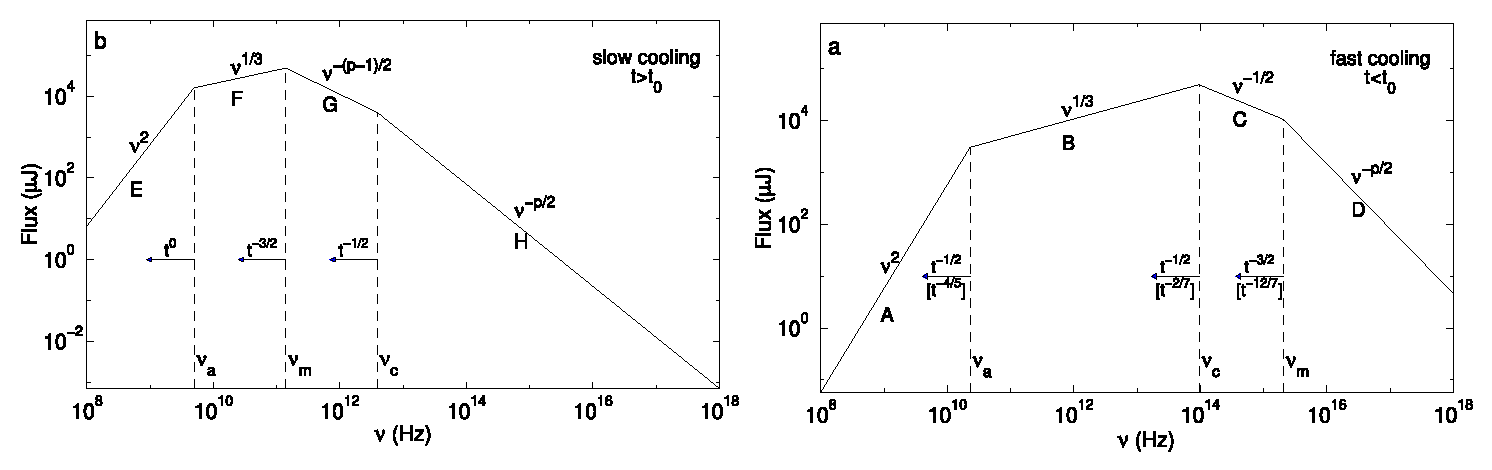
\includegraphics[height=4.8cm]{figures/sari97_flat.pdf}
            }};
        }
    \end{tikzpicture}
\end{frame}
%%% --------------------------------------------------------------
%%
%% R E S U L T S
%%
%% --------------------------------------------------------------

\section{Preliminary Results}
\subsection{Modelling sGRB afterglow (GRB170817A)}
\begin{frame}{}  %% ---------- Intro/motivation 
    \begin{tikzpicture}[overlay,remember picture]
        \uncover<1->{ % <-> |
            \node (t1) [anchor=center,scale=1,opacity=1] at ([shift={(-3.0cm,2.5cm)}]current page.center){
                \parbox{0.7\textwidth}{
                    \begin{itemize}
                        \item Gaussian jet $E(\theta) \propto e^{(\theta/\theta_c)^2}$
                        \item Off-axis $\theta_{\rm obs} > \theta_c$
                        \item Relativistic core, $\Gamma_c \sim 10^2$; low ISM density.
                    \end{itemize}
            }};
        }
        \uncover<1->{ % <-> |
            \node (img1) [anchor=center,scale=1,opacity=1] at ([shift={(1.cm,-1.35cm)}]current page.center){
                \parbox{1.0\textwidth}{
                    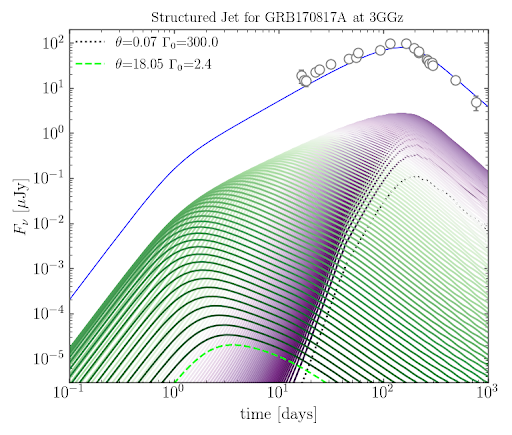
\includegraphics[height=6cm]{figures/grb170817fernandezPyBlastAfterglow.png}
            }};
        }
        \uncover<1->{ % <-> |
            \node (img1) [anchor=center,scale=1,opacity=1] at ([shift={(9.0cm,-0.5cm)}]current page.center){
                \parbox{1.0\textwidth}{
                    Flux centroid motion, $4.5\,$GGz; \\
                    Color is $I/I_{\rm max}$ %is shown with $I=0.01I_{\rm max}$ cut
                    
                    \movie[width=0.8\textwidth]{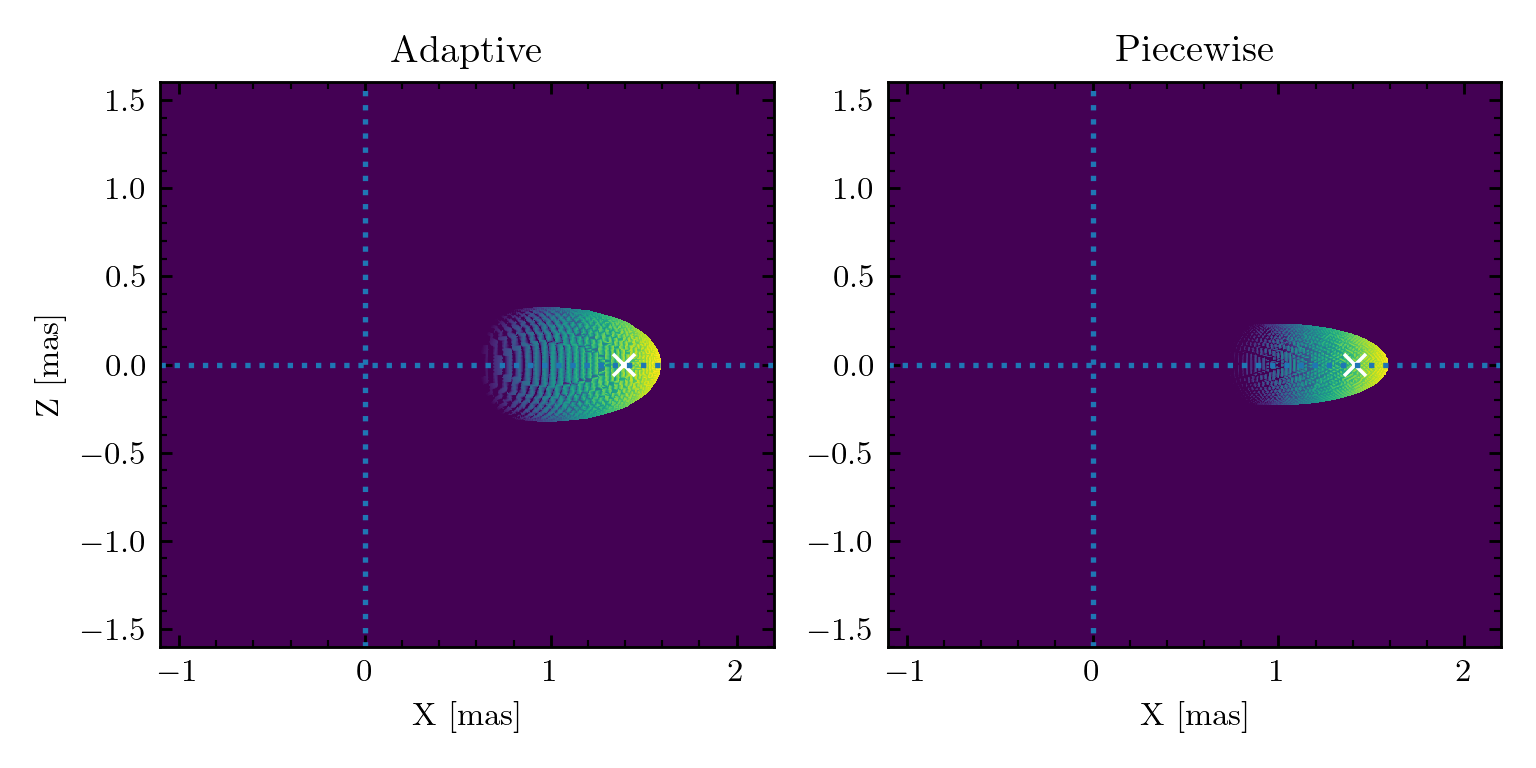
\includegraphics[width=0.8\textwidth]{figures/200.png}}{figures/out2.mp4}
            }};
        }
    \end{tikzpicture}
\end{frame}


% =============================================================================================

\subsection{Kilonova afterglow for NR ejecta profiles}
\begin{frame}{}  %% ---------- Intro/motivation 
    \begin{tikzpicture}[overlay,remember picture]
        \uncover<1->{ % <-> |
            \node (t1) [anchor=center,scale=1,opacity=1] at ([shift={(-3.1cm,-0.5cm)}]current page.center){
                \parbox{0.65\textwidth}{
                    %                    \textbf{Main Features}:
                    \begin{itemize}
                        \item Set of NS BNS simulations targeted to \GW{}.
                        %
                        \item BNS model $(q,\tilde{\Lambda})$ $q=M_A/M_B$ is the mass ratio, $\tilde{\Lambda}$ tidal deformability parameter (Depends in EOS of NS)
                        %
                        \item Ejecta $M,\beta,E_k = f(q,\tilde{\Lambda})$
                        %
                    \end{itemize}
                    
                    \textbf{Assuming that GRB170817A change in afterglow is due to the emergence of a new component}: 
                    \begin{itemize}
                        \item New way to constrain binary parameters, EOS
                        %
                        \item Additional information on ISM
                        %
                        \item Information on shock physics
                        %
                    \end{itemize}
            }};
        }
        \uncover<1-1>{ % <-> |
            \node (img1) [anchor=center,scale=1,opacity=1] at ([shift={(5.0cm,1.8cm)}]current page.center){
                \parbox{0.5\textwidth}{
                    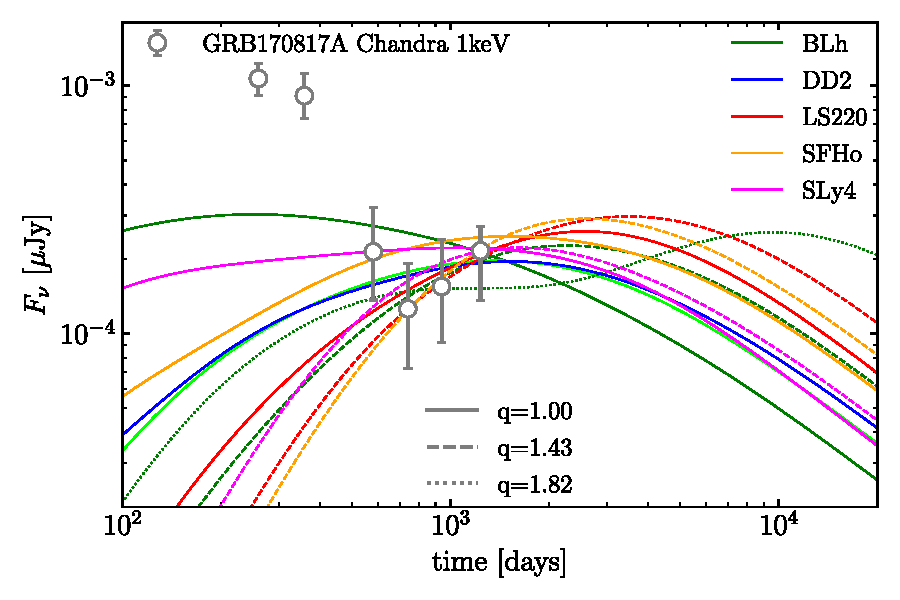
\includegraphics[height=3.8cm]{figures/best_xray_obs_representative_all_eos.pdf}
                    
                    %\small{\textbf{Artist depiction of ejecta$^\text{\citep{Ascenzi:2020xqi}}$}}
            }};
        }
        \uncover<1-1>{ % <-> |
            \node (img1) [anchor=center,scale=1,opacity=1] at ([shift={(5.2cm,-2.2cm)}]current page.center){
                \parbox{0.5\textwidth}{
                    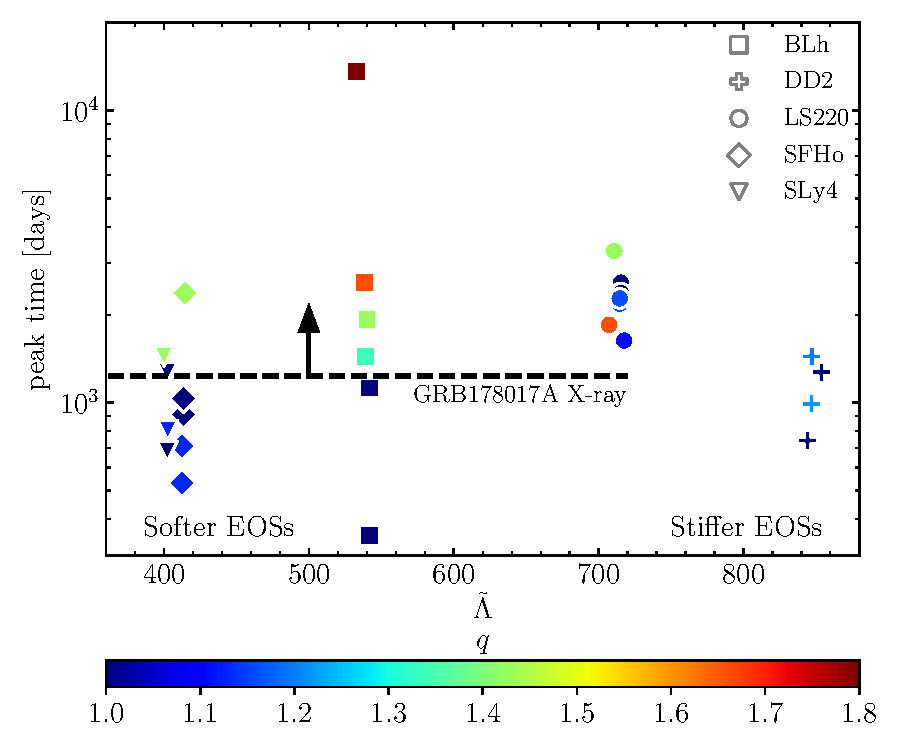
\includegraphics[height=4.2cm]{figures/scatter_lightcurve_tpeak_vs_lambda.pdf}
                    
                    %\small{\textbf{Artist depiction of ejecta$^\text{\citep{Ascenzi:2020xqi}}$}}
            }};
        }
    \end{tikzpicture}
\end{frame}

% =============================================================================================

\subsection{Thermal electrons in mildly relativistic shocks}
\begin{frame}{}  %% ---------- Intro/motivation 
    \begin{tikzpicture}[overlay,remember picture]
        \uncover<1->{ % <-> |
            \node (t1) [anchor=center,scale=1,opacity=1] at ([shift={(-3.0cm,2.2cm)}]current page.center){
                \parbox{0.5\textwidth}{
                    \begin{itemize}
                        \item ``Thermal spectrum'' (left)
                        \item ``Non-thermal spectrum'' (right)
                    \end{itemize}
                    $\beta_{\rm sh}=0.1$, $n_{\rm ISM}=10^4\,\ccm$, $t=200\,$d, $\delta=0.1$, $p=3$, $B=0.1\,$G, $\varepsilon_T=0.1$
            }};
        }
        \uncover<1->{ % <-> |
            \node (t1) [anchor=center,scale=1,opacity=1] at ([shift={(4.0cm,2.2cm)}]current page.center){
                \parbox{0.5\textwidth}{
                    \begin{eqnarray*}
                        \frac{\partial N}{\partial \gamma}\Big|_{\rm th} &= n_{e} \frac{ \gamma^2\sqrt{1-\gamma^{-2}} }{K_2(1/\Theta) \Theta} e^{-\gamma/\Theta}, \\
                        %                        \hspace{5mm}
                        \frac{\partial N}{\partial \gamma}\Big|_{\rm pl} &= n_e g(\Theta)\delta\frac{p-2}{3\Theta}\Big(\frac{\gamma}{3\Theta}\Big)^{-p}
                    \end{eqnarray*}
                    
                    
                    %                    Spectrum $3$ segments: 
                    %                    (i) $\nu < \nu_c$: low energy tail, $F_{\nu}\propto\nu^{1/3}$, 
                    %                    (ii) $\nu(\gamma) > \nu_c$ power law segment $F_{\nu}\propto\nu^{-1/2}$ 
                    %                    (iii) $\nu(\gamma)$and 
            }};
        }
        \uncover<1->{ % <-> |
            \node (img1) [anchor=center,scale=1,opacity=1] at ([shift={(2.cm,-1.5cm)}]current page.center){
                \parbox{1.0\textwidth}{
                    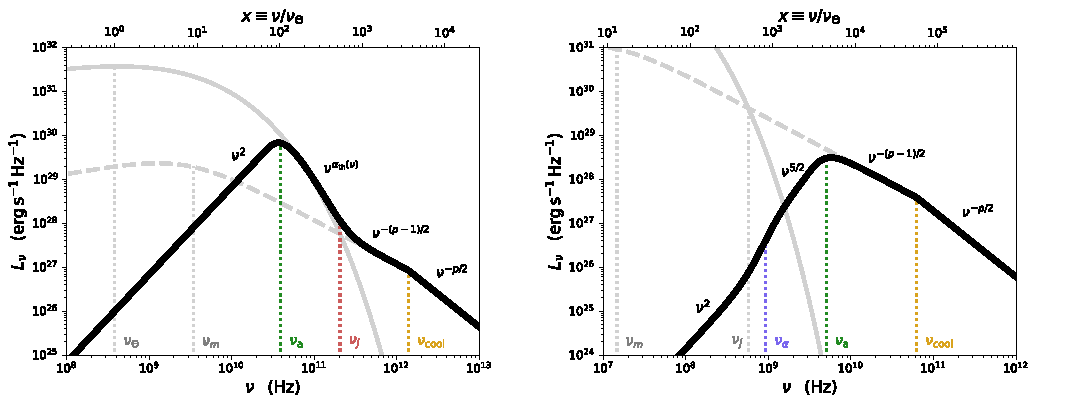
\includegraphics[height=5cm]{figures/Margalit21_thermalElectrons.pdf}
            }};
        }
    \end{tikzpicture}
\end{frame}
\begin{frame}{}  %% ---------- Intro/motivation 
    \begin{tikzpicture}[overlay,remember picture]
        \uncover<1->{ % <-> |
            \node (t1) [anchor=center,scale=1,opacity=1] at ([shift={(-5.0cm,1.2cm)}]current page.center){
                \parbox{0.4\textwidth}{
                    Comparison between two optically thin ight cruves:
                    \begin{itemize}
                        \item ``Thermal'' (blue)
                        \item ``Non-thermal'' (green)
                    \end{itemize}
                    Further investigations required! 
            }};
        }
        \uncover<1->{ % <-> |
            \node (img1) [anchor=center,scale=1,opacity=1] at ([shift={(6.cm,0.0cm)}]current page.center){
                \parbox{1.0\textwidth}{
                    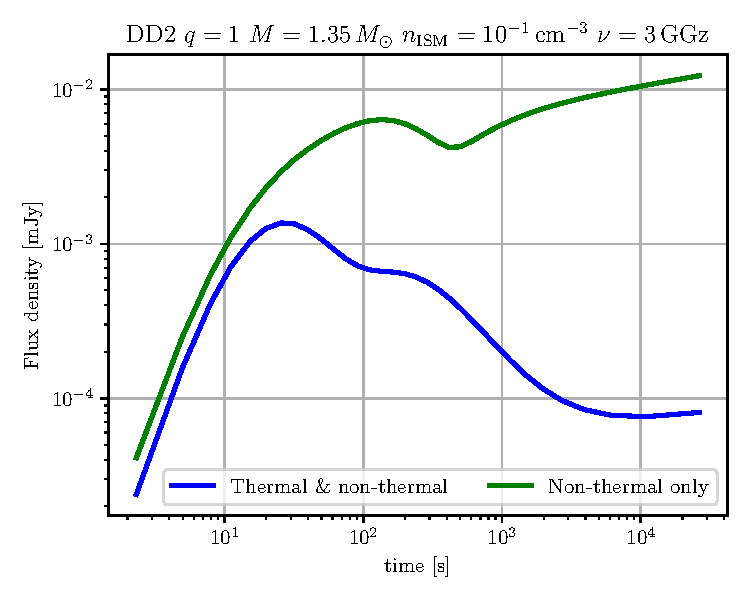
\includegraphics[height=7cm]{figures/test_thermal_electrons.pdf}
            }};
        }
    \end{tikzpicture}
\end{frame}

% =============================================================================================

\subsection{Extracting kilonova ejecta profile}
\begin{frame}{}  %% ---------- Intro/motivation 
    \begin{tikzpicture}[overlay,remember picture]
        \uncover<1->{ % <-> |
            \node (t1) [anchor=center,scale=1,opacity=1] at ([shift={(-3.0cm,2.5cm)}]current page.center){
                \parbox{0.7\textwidth}{
                    \begin{itemize}
                        \item $E_{\rm k} = f(\theta,\beta)$
                        \item $E_{\rm k;max}$ at $\theta\rightarrow0$ and $\beta\rightarrow0.2$.
                        \item $\log_{10}(E_k)=b_0 + (b_1 \theta) + (b_2 \beta) + (b_3 \theta^2) + (b_4 \theta \beta) + (b_5 \beta^{1/4})$
                    \end{itemize}
            }};
        }
        \uncover<1->{ % <-> |
            \node (img1) [anchor=center,scale=1,opacity=1] at ([shift={(2.2cm,-1.35cm)}]current page.center){
                \parbox{1.0\textwidth}{
                    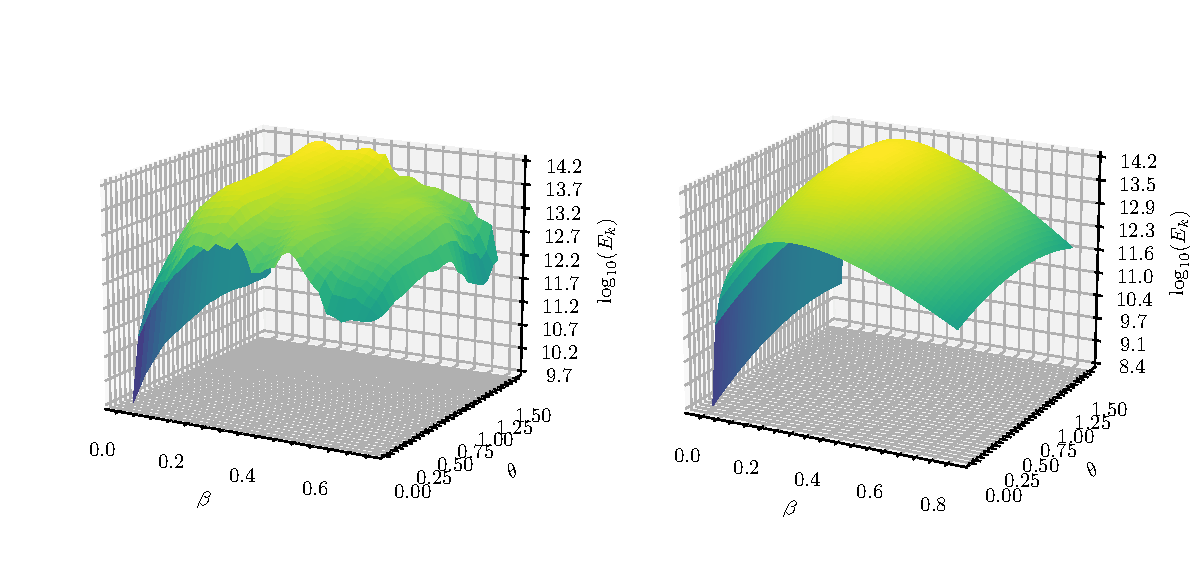
\includegraphics[height=6cm]{figures/fit_2d_ejecta.pdf}
            }};
        }
        \uncover<1->{ % <-> |
            \node (img1) [anchor=center,scale=1,opacity=1] at ([shift={(9cm,2cm)}]current page.center){
                \parbox{1.0\textwidth}{
                    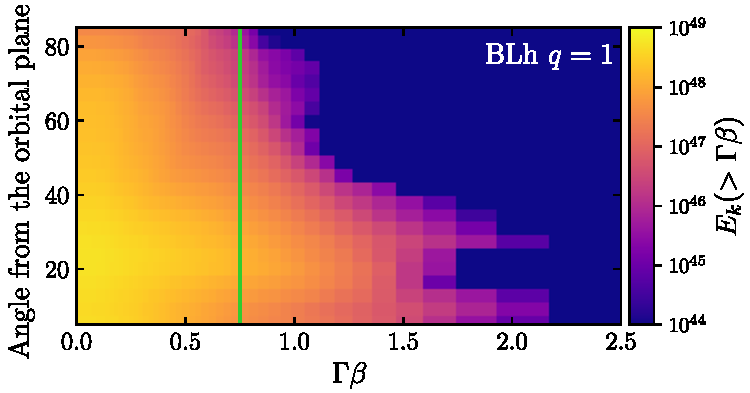
\includegraphics[height=3cm]{figures/kinetic_energy_struct_models_bottom_only.pdf}
            }};
        }
    \end{tikzpicture}
\end{frame}

% =============================================================================================

\subsection{Dynamics in the toy model}
\begin{frame}{}  %% ---------- Intro/motivation 
    \begin{tikzpicture}[overlay,remember picture]
        \uncover<1->{ % <-> |
            \node (t1) [anchor=center,scale=1,opacity=1] at ([shift={(-4.8cm,1.2cm)}]current page.center){
                \parbox{0.45\textwidth}{
                    kN ejecta expands into ISM 'processed' by GRB
                    Three possible scenaria 
                    \begin{itemize}
                        \item kN ejecta behind \& inside the GRB one
                        \item kN ejecta behind \& outside the GRB one
                        \item kn ejecta ahead of the GRB one
                    \end{itemize}
                    Further investigations required! 
            }};
        }
        
        \uncover<2->{ % <-> |
            \node (t1) [anchor=center,scale=1,opacity=1] at ([shift={(-4.8cm,-2.6cm)}]current page.center){
                \parbox{0.45\textwidth}{
                    \textcolor{red}{Error!} 
                    Shells $\Gamma_{\rm jet} = \Gamma_{\rm ej}$ at $R_{\rm jet}=R_{\rm ej}$ 
                    at \textbf{different} times.
                    
                    Consier a toy model 
                    ($1$ ejectan and $1$ jet spherical shell)
            }};
        }
        
        \uncover<1->{ % <-> |
            \node (img1) [anchor=center,scale=1,opacity=1] at ([shift={(6.cm,0.0cm)}]current page.center){
                \parbox{1.0\textwidth}{
                    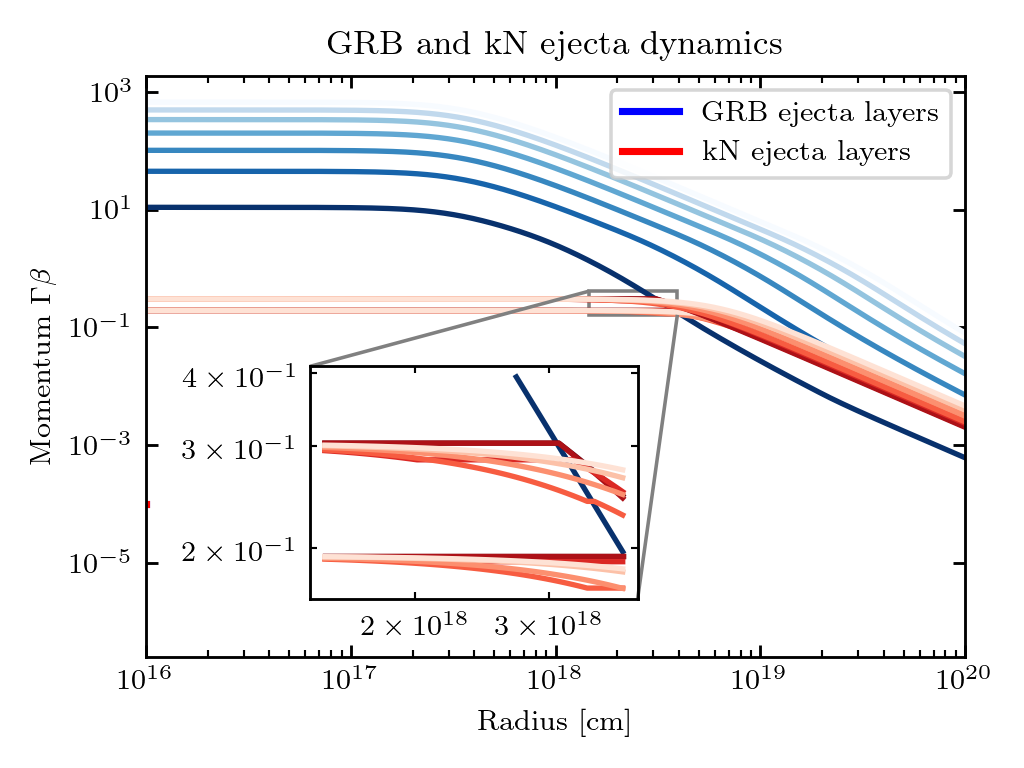
\includegraphics[height=7cm]{figures/plot_pretty_dynamics.png}
            }};
        }
    \end{tikzpicture}
\end{frame}

% =============================================================================================

\subsection{Dynamics in the toy model [Incl. density behind slowed GRB BW]}
\begin{frame}{}  %% ---------- Intro/motivation 
    \begin{tikzpicture}[overlay,remember picture]
        \uncover<1-1>{ % <-> |
            \node (t1) [anchor=center,scale=1,opacity=1] at ([shift={(-4.8cm,2.2cm)}]current page.center){
                \parbox{0.42\textwidth}{
                    Improving shell interaction
                    \begin{itemize}
                        \item $dU/dR\rightarrow dU/dt_b$ where $U\in\{R,\Gamma,E_{\rm int}...\}$, $t_b$ is time in burster frame. Shell "collide" at $t_{\rm coll}$, $R_{\rm jet} = R_{\rm ej}$. 
                    \end{itemize}
            }};
        }
        \uncover<1-1>{ % <-> |
        \node (t1) [anchor=center,scale=1,opacity=1] at ([shift={(-4.8cm,-2.2cm)}]current page.center){
            \parbox{0.42\textwidth}{
                What happens at shell collision?
        }};
        } 
        \uncover<3-5>{ % <-> |
        \node (t1) [anchor=center,scale=1,opacity=1] at ([shift={(-4.8cm,1.2cm)}]current page.center){
            \parbox{0.42\textwidth}{
                Improving shell interaction
                \begin{itemize}
                    \item $dU/dR\rightarrow dU/dt_b$ where $U\in\{R,\Gamma,E_{\rm int}...\}$, $t_b$ is time in burster frame. Shell "collide" at $t_{\rm coll}$, $R_{\rm jet} = R_{\rm ej}$. 
                    \item Behind the BW $\rho$ is low but $\rho\neq0$. Consider Taylor-von Neumann-Sedov BW. 
                \end{itemize}
        }};
        }
        \uncover<1-1>{ % <-> |
            \node (img1) [anchor=center,scale=1,opacity=1] at ([shift={(5.0cm,0.0cm)}]current page.center){
                \parbox{1.0\textwidth}{
                    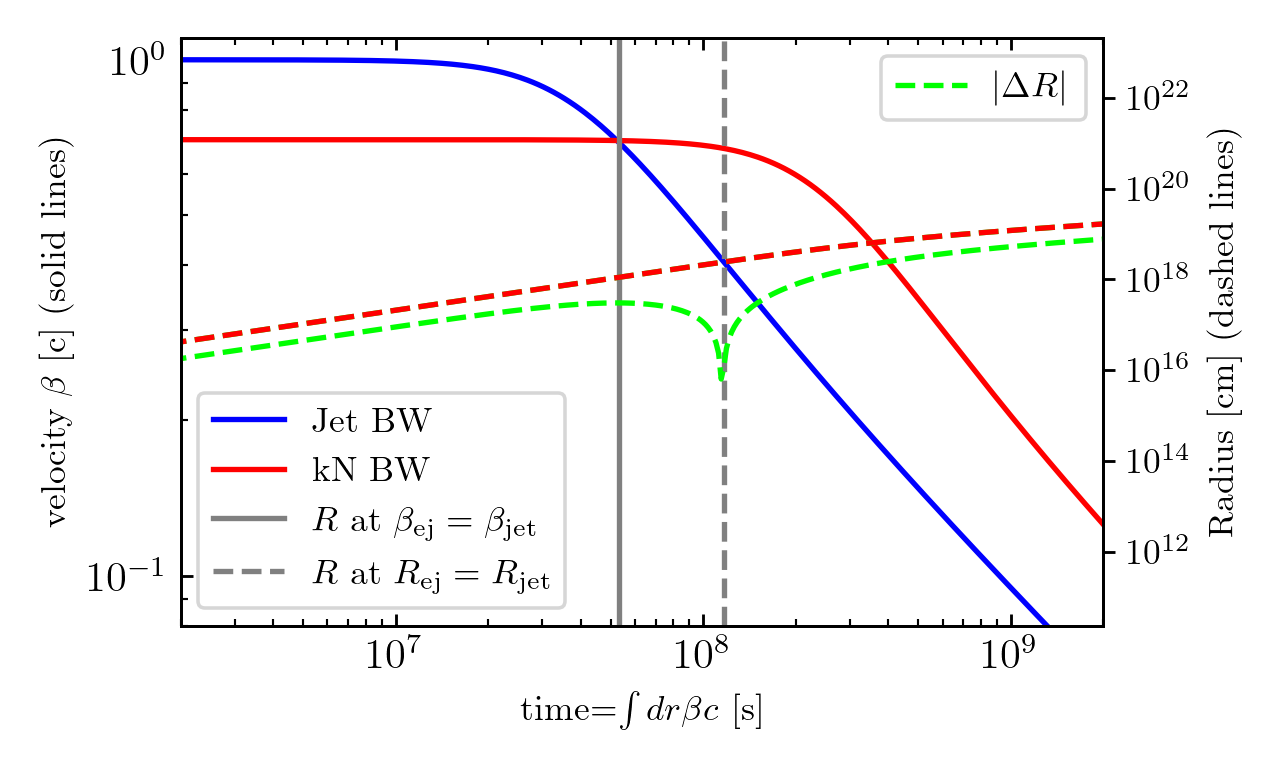
\includegraphics[height=6.0cm]{figures/time_intersection.png}
            }};
        }
        \uncover<2-2>{ % <-> |
            \node (t1) [anchor=center,scale=1,opacity=1] at ([shift={(0.0cm,-0.2cm)}]current page.center){
                \parbox{0.80\textwidth}{
                    What happens at collision of shells?
                    \begin{eqnarray*}
                        T^{\mu\nu} &=& (\rho' c^2 + \omega' p')u^{\mu}u^{\nu} + p'\eta^{\mu\nu} \\
                        E_{\rm tot} &=& \int{T^{00}}dV = \Gamma m + \Gamma_{\rm eff}(\hat{\gamma})E_{\rm int}'\\
                        P^{i} &=& c\sqrt{\Gamma^2 - 1} (m + \hat{\gamma}E_{\rm int}' / c^2 ) 
                    \end{eqnarray*}
                    Energy and momentum conservation at the collision of $2$ shells:
                    \begin{eqnarray*}
                        E_{\rm tot; f} &=& E_{\rm tot; 1} + E_{\rm tot; 2} \\
                        P_{\rm f} &=& P_{1} + P_{2}
                    \end{eqnarray*}
                    Non-linear system of equations that gives the 
                    initial state, $\Gamma_f$ and $E_{\rm int;f }'$  of the 'merged' shell.
                    
                    \textcolor{green}{Possible for two simple shells} \\
                    \textcolor{red}{Impossible for structured\&spreading shells -- Dead End}
            }};
        }
        \uncover<3-3>{ % <-> |
            \node (img1) [anchor=center,scale=1,opacity=1] at ([shift={(5.0cm,0.0cm)}]current page.center){
                \parbox{1.0\textwidth}{
                    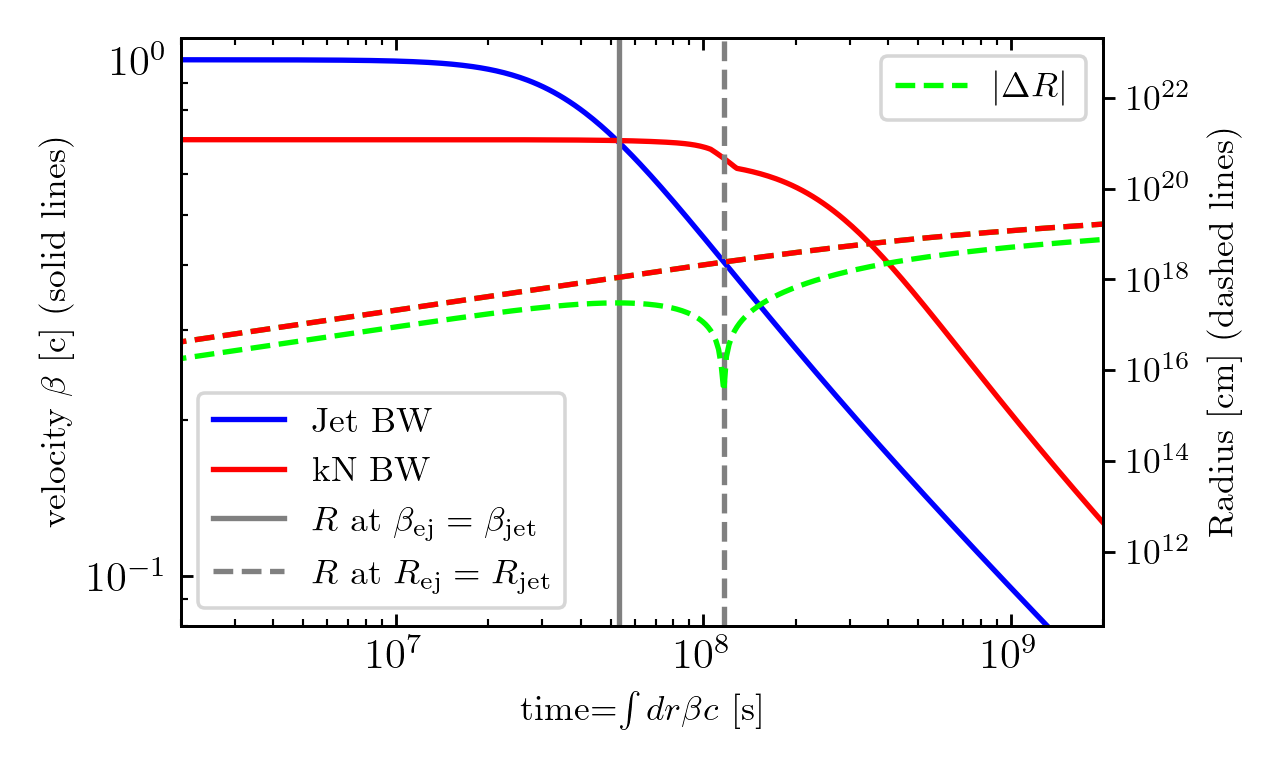
\includegraphics[height=6.0cm]{figures/time_intersection2.png}
            }};
        }
        
        
        \uncover<4-4>{ % <-> |
        \node (img1) [anchor=center,scale=1,opacity=1] at ([shift={(5.0cm,0.1cm)}]current page.center){
            \parbox{1.0\textwidth}{
                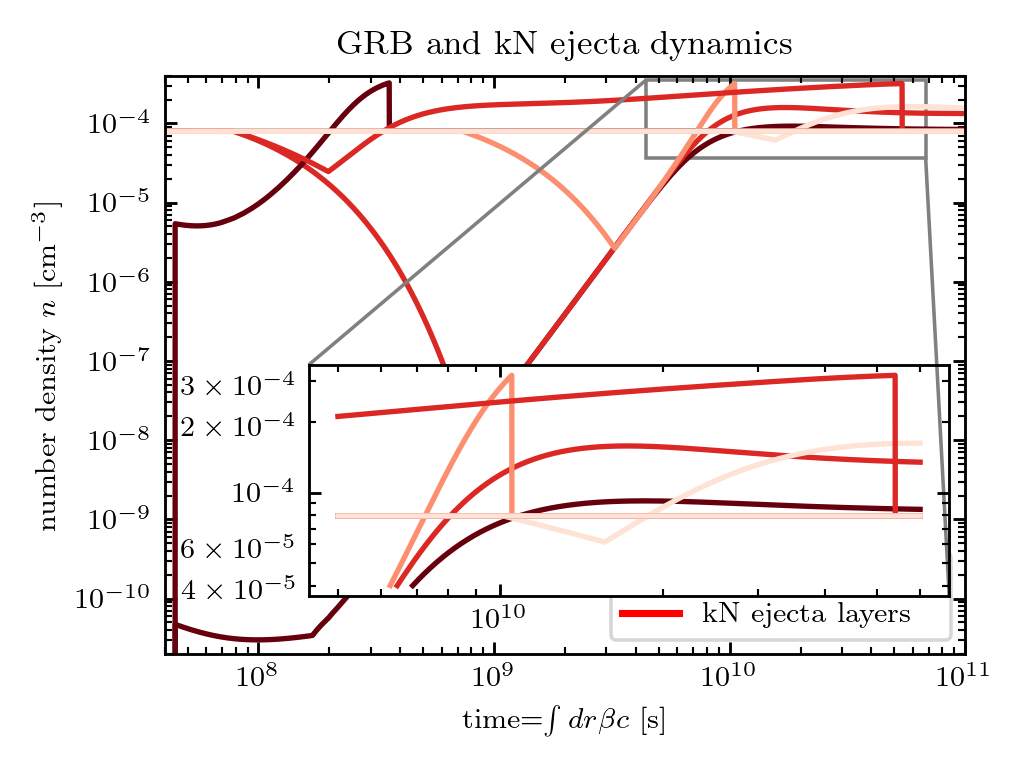
\includegraphics[height=7.0cm]{figures/plot_pretty_dynamics_rho_full.png}
        }};
        }
        \uncover<5-5>{ % <-> |
            \node (img1) [anchor=center,scale=1,opacity=1] at ([shift={(5.0cm,0.1cm)}]current page.center){
                \parbox{1.0\textwidth}{
                    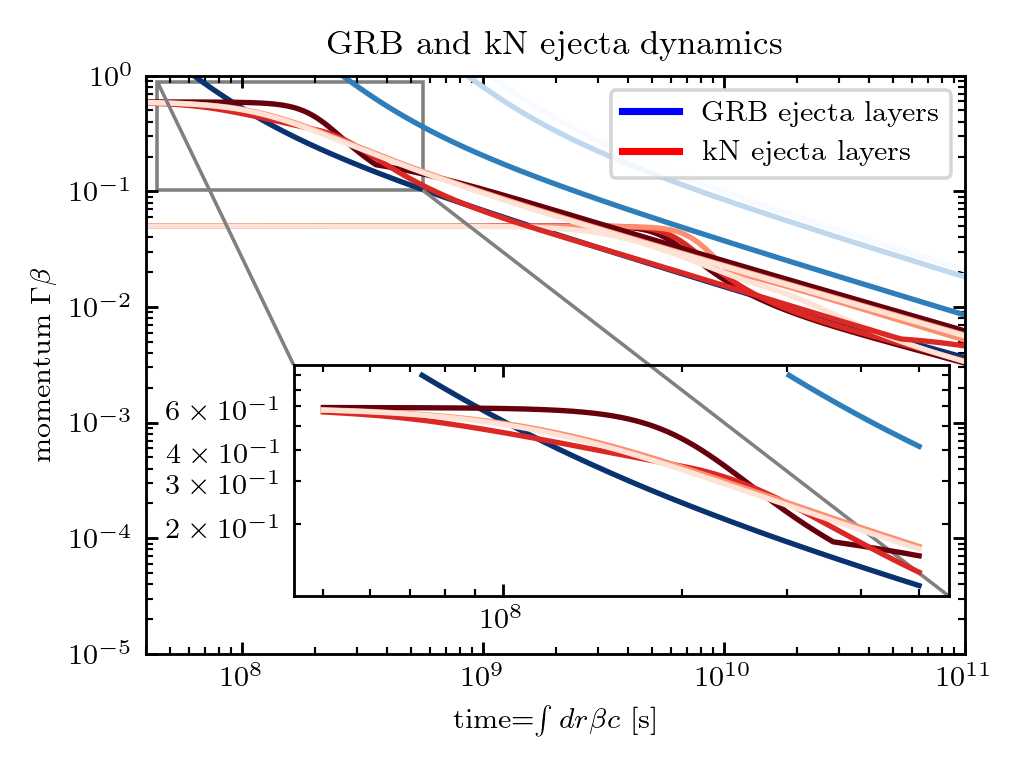
\includegraphics[height=7.0cm]{figures/plot_pretty_dynamics_full.png}
            }};
        }
        \uncover<3-5>{ % <-> |
        \node (img1) [anchor=center,scale=1,opacity=1] at ([shift={(-0.0cm,-2.4cm)}]current page.center){
            \parbox{1.0\textwidth}{
                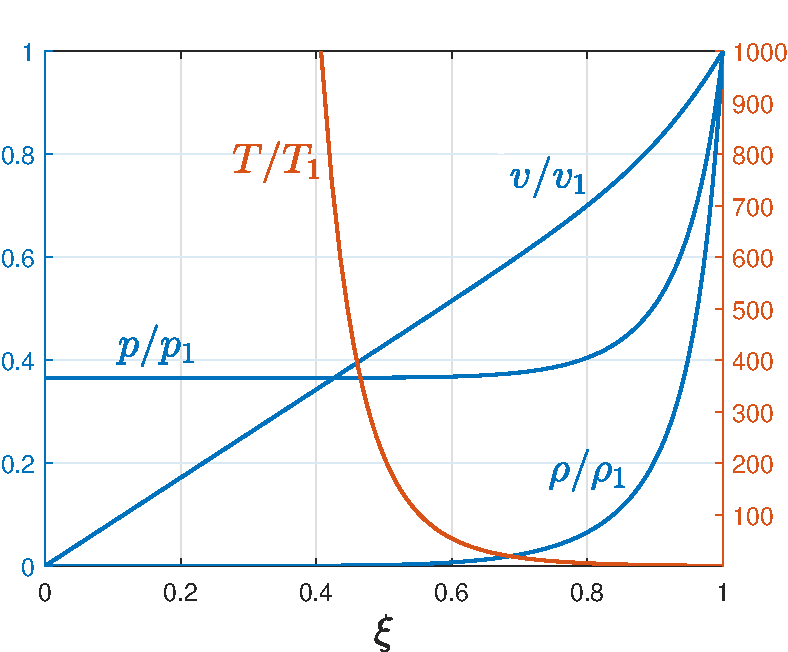
\includegraphics[height=3.5cm]{figures/TNS_blast_wave.pdf}
        }};
    
        }
        \uncover<3-3>{ % <-> |
        \node (t1) [anchor=center,scale=1,opacity=1] at ([shift={(3.5cm,-3.6cm)}]current page.center){
            \parbox{0.60\textwidth}{
                \textcolor{red}{Major code change: jet and ejecta BWs have to solved together}.
        }};
        }
        \uncover<4-4>{ % <-> |
        \node (t1) [anchor=center,scale=1,opacity=1] at ([shift={(3.5cm,-3.6cm)}]current page.center){
            \parbox{0.60\textwidth}{
                \textcolor{green}{Major code change: jet and ejecta BWs have to solved together}.
        }};
        }
        \uncover<5-5>{ % <-> |
            \node (t1) [anchor=center,scale=1,opacity=1] at ([shift={(3.5cm,-3.6cm)}]current page.center){
                \parbox{0.60\textwidth}{
                    \textcolor{orange}{Missing: effect of the realtive vlocity $\beta_{12}=\frac{\beta_1 - \beta_2}{1 - \beta_1\beta_2}$}.
            }};
        }
        \uncover<6-6>{ % <-> |
        \node (t1) [anchor=center,scale=1,opacity=1] at ([shift={(-1.0cm,-0.0cm)}]current page.center){
            \parbox{0.99\textwidth}{
                Derive dynamics of a fluid expanding in a non-uniform, pre-accelerate ISM
                \begin{equation*}
                    \begin{aligned}
                        T^{\mu\nu} =& (\rho' c^2 + e' p')u^{\mu}u^{\nu} + p'\eta^{\mu\nu}, \, p' = (\hat{\gamma}-1)(e'- \rho' c^2), \, E_{\rm int} = (e' - \rho'c^2)V' \\ 
                        E_{\rm tot} =& \int{T^{00}}dV = \Big(\Gamma^2\rho' c^2 + (\hat{\gamma}\Gamma^2-\hat{\gamma}+1)e'\Big) \frac{V'}{\Gamma} = \Gamma m + \Gamma_{\rm eff}(\hat{\gamma})E_{\rm int}'\\
                        dE_{\rm tot} =& 0 \rightarrow d [ \Gamma (M_0 + m) c^2 + \Gamma_{\rm eff}E_{\rm int}' ] = \Gamma_{\rm ISM} dm c^2 + \Gamma_{\rm eff} dE_{\rm rad}' \\
                        dE_{\rm int} =& dE_{\rm sh} + dE_{\rm ad} + dE_{\rm rad} \\
                        dE_{\rm sh} =& (\Gamma_{\rm rel}-1) dm c^2, \, \Gamma_{\rm rel} = \Gamma\Gamma_{\rm ISM}(1-\beta\beta_{\rm ISM}\rm) \\
                        dE_{\rm ad} =& - p dV + TdS = -(\hat{\gamma}-1)(E_{\rm int}'/V') dV' = -(\hat{\gamma}-1)E_{\rm int}' d\ln V' \\
%                        V' \propto R^3 \Gamma_{\rm ISM} / \Gamma_{\rm rel}; \\
%                        d\ln V' =& d\ln m - d\ln\rho - d\ln\Gamma_{\rm rel} + d\ln\Gamma_{\rm ISM}\\
                        \frac{d\Gamma}{dR} &= \frac{ -(\Gamma-\Gamma_{\rm ISM} + \Gamma_{\rm eff} (\Gamma_{\rm rel}-1)) + \Gamma_{\rm eff}(\hat{\gamma}-1)E_{\rm int}' \Big( \frac{dm}{dR}\frac{1}{m} - 
                        \textcolor{red}{\frac{d\rho_{\rm ISM}}{dR}}\frac{1}{\rho_{\rm ISM}} -
                        \textcolor{red}{\frac{d\Gamma_{\rm ISM}}{dR}}\frac{1}{\Gamma_{\rm ISM}} \Big) }{ (M_0 + m)c^2 + \frac{d\Gamma_{\rm eff}}{d\Gamma}E_{\rm int}' + \Gamma_{\rm eff}(\hat{\gamma}-1)E_{\rm int}' 
                        \textcolor{red}{\frac{d\Gamma_{\rm rel}}{d\Gamma}}\frac{1}{\Gamma_{\rm rel}} },
                    \end{aligned}
                \end{equation*}
%                \begin{eqnarray*}
%                    T^{\mu\nu} &=& (\rho' c^2 + \omega' p')u^{\mu}u^{\nu} + p'\eta^{\mu\nu} \\
%                    E_{\rm tot} &=& \int{T^{00}}dV = \Gamma m + \Gamma_{\rm eff}(\hat{\gamma})E_{\rm int}'\\
%                    P^{i} &=& c\sqrt{\Gamma^2 - 1} (m + \hat{\gamma}E_{\rm int}' / c^2 ) 
%                \end{eqnarray*}
%                Energy and momentum conservation at the collision of $2$ shells:
%                \begin{eqnarray*}
%                    E_{\rm tot; f} &=& E_{\rm tot; 1} + E_{\rm tot; 2} \\
%                    P_{\rm f} &=& P_{1} + P_{2}
%                \end{eqnarray*}
%                Non-linear system of equations that gives the 
%                initial state, $\Gamma_f$ and $E_{\rm int;f }'$  of the 'merged' shell.
%                
%                \textcolor{green}{Possible for two simple shells} \\
%                \textcolor{red}{Impossible for structured\&spreading shells -- Dead End}
        }};
    }
    \end{tikzpicture}
\end{frame}

% =============================================================================================

\subsection{Complex shell dynamics}
\begin{frame}{}  %% ---------- Intro/motivation 
    \begin{tikzpicture}[overlay,remember picture]
        \uncover<1->{ % <-> |
            \node (t1) [anchor=center,scale=1,opacity=1] at ([shift={(-4.5cm,1.2cm)}]current page.center){
                \parbox{0.45\textwidth}{
                    Dynamics of the kilonova ejecta, 
                    shaped by the GRB jet \\ 
                    
                    Left two panels: \\
                    Interaction with slowest GRB layer \\
                    
                    Right two panels: \\
                    Interaction with fastest GRB layer
                    
                    Top panels: 
                    
                    
            }};
        }
        \uncover<1->{ % <-> |
            \node (img1) [anchor=center,scale=1,opacity=1] at ([shift={(6.1cm,1.7cm)}]current page.center){
                \parbox{1.0\textwidth}{
                    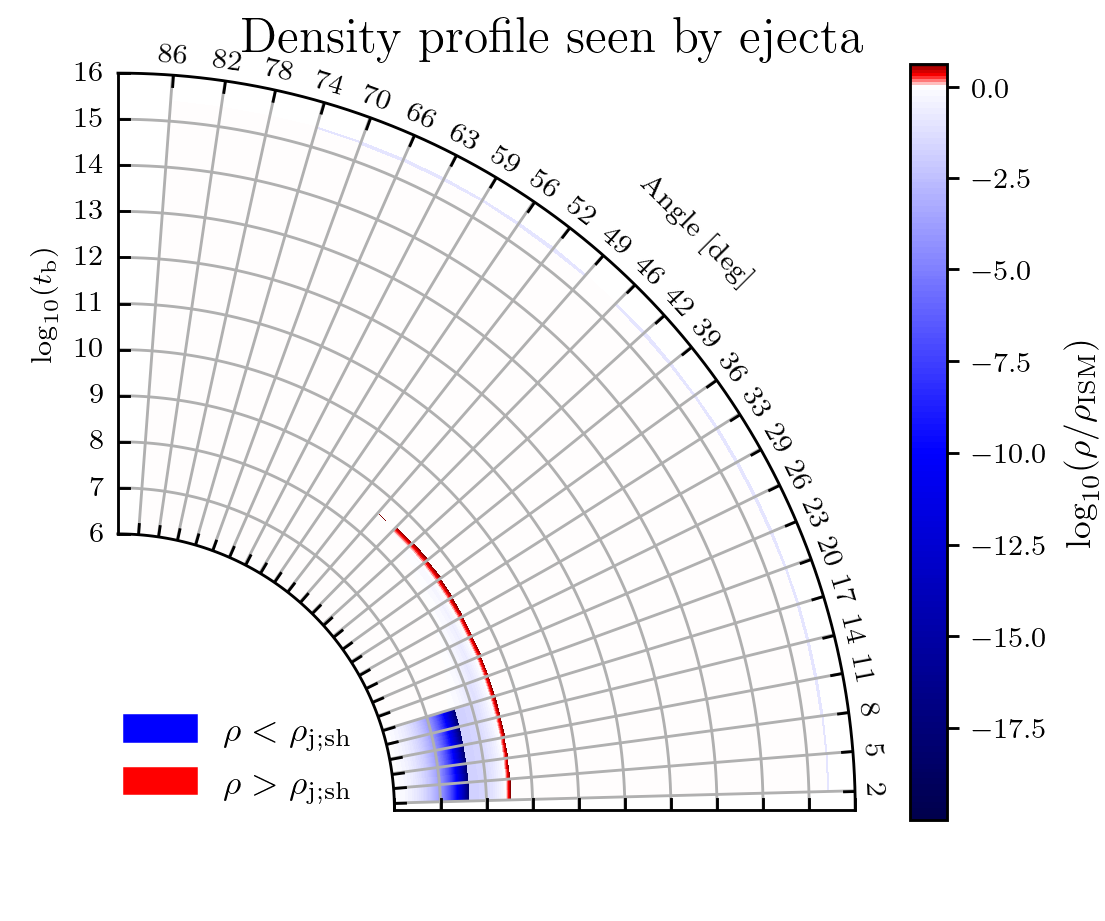
\includegraphics[height=4cm]{figures/bw_ej_dens_ism_evol_slow_shell_2.png}
            }};
        }
        \uncover<1->{ % <-> |
            \node (img1) [anchor=center,scale=1,opacity=1] at ([shift={(6.1cm,-2.3cm)}]current page.center){
                \parbox{1.0\textwidth}{
                    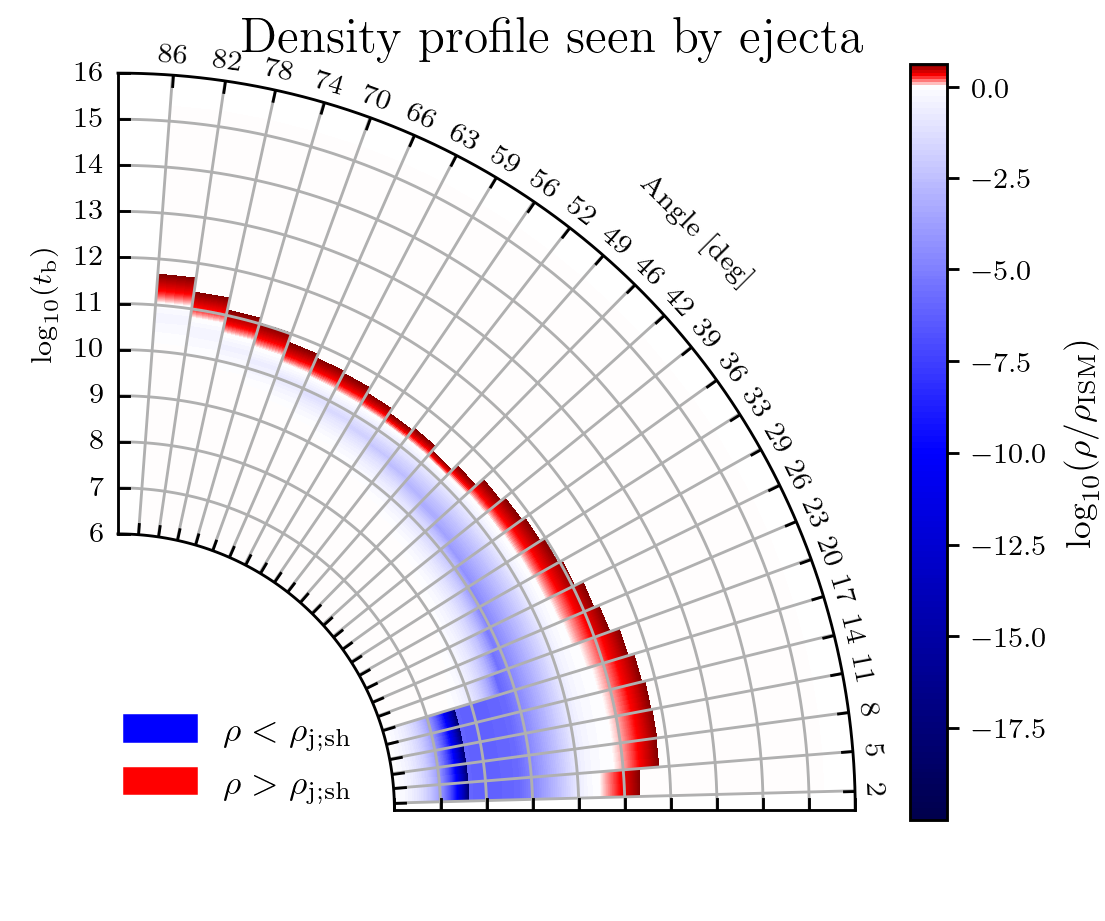
\includegraphics[height=4cm]{figures/bw_ej_dens_ism_evol_fast_shell_2.png}
            }};
        }
        \uncover<1->{ % <-> |
            \node (img1) [anchor=center,scale=1,opacity=1] at ([shift={(10.cm,1.7cm)}]current page.center){
                \parbox{1.0\textwidth}{
                    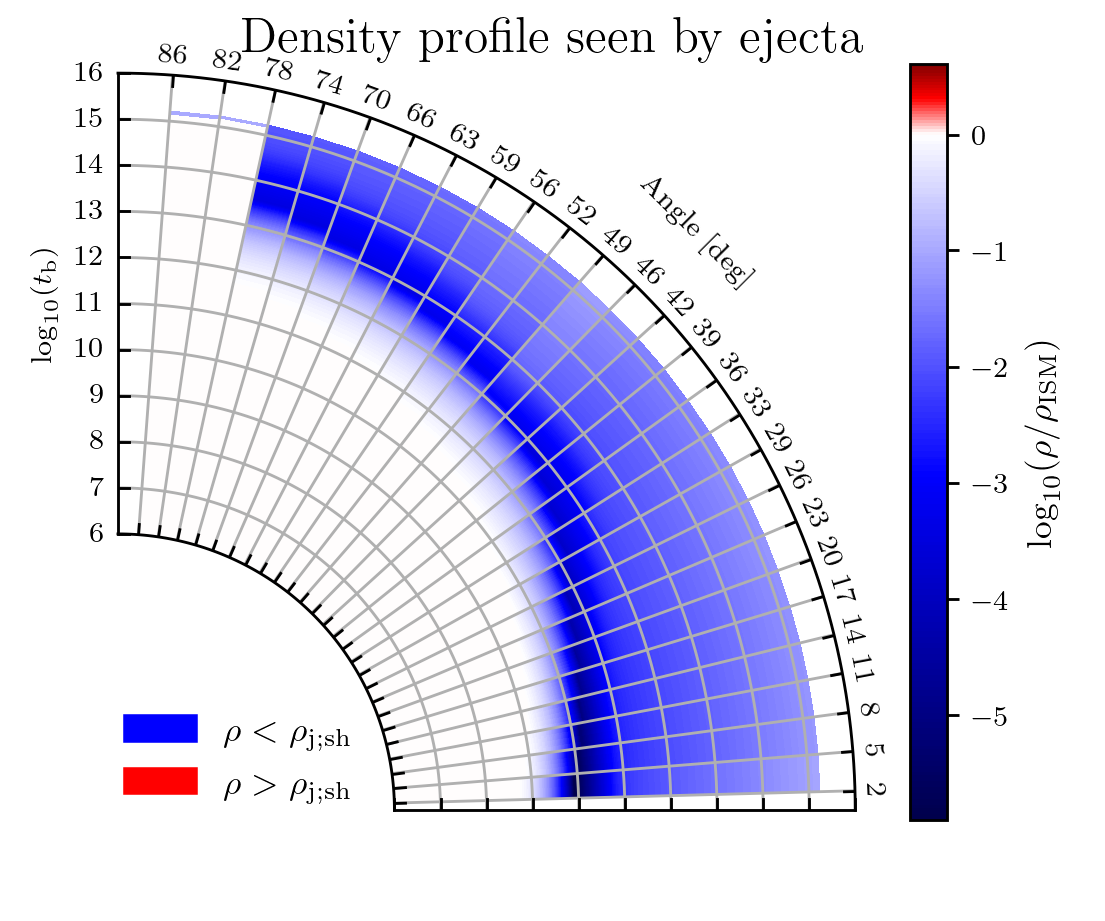
\includegraphics[height=4cm]{figures/bw_ej_dens_ism_evol_slow_shell.png}
            }};
        }
        \uncover<1->{ % <-> |
            \node (img1) [anchor=center,scale=1,opacity=1] at ([shift={(10.cm,-2.3cm)}]current page.center){
                \parbox{1.0\textwidth}{
                    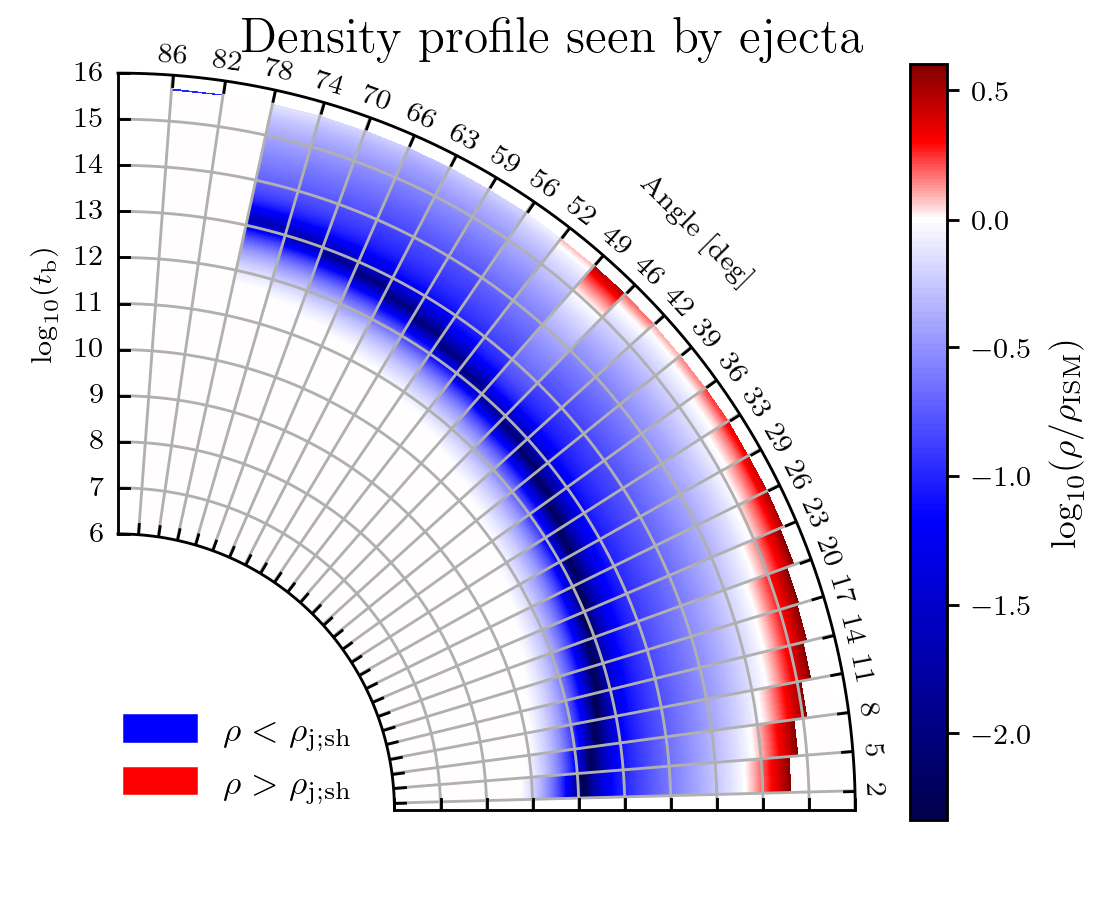
\includegraphics[height=4cm]{figures/bw_ej_dens_ism_evol_fast_shell.png}
            }};
        }
    \end{tikzpicture}
\end{frame}

% =============================================================================================

\subsection{Sky Images}
\begin{frame}{}  %% ---------- Intro/motivation 
    \begin{tikzpicture}[overlay,remember picture]
        \uncover<1->{ % <-> |
            \node (t1) [anchor=center,scale=1,opacity=1] at ([shift={(-4.5cm,1.2cm)}]current page.center){
                \parbox{0.45\textwidth}{
                    Sky image: 
                    
                    for the jet shows the motion of the flux centroid -- constraining inclanation
                    For the ejecta traces its angular deistribution (\textcolor{red}{if resolved})
                    
                    Further investigations required! 
                    
                    Is it possible to observe with very-long-base-line interferometers?
            }};
        }
        \uncover<1->{ % <-> |
            \node (img1) [anchor=center,scale=1,opacity=1] at ([shift={(6.cm,1.7cm)}]current page.center){
                \parbox{1.0\textwidth}{
                    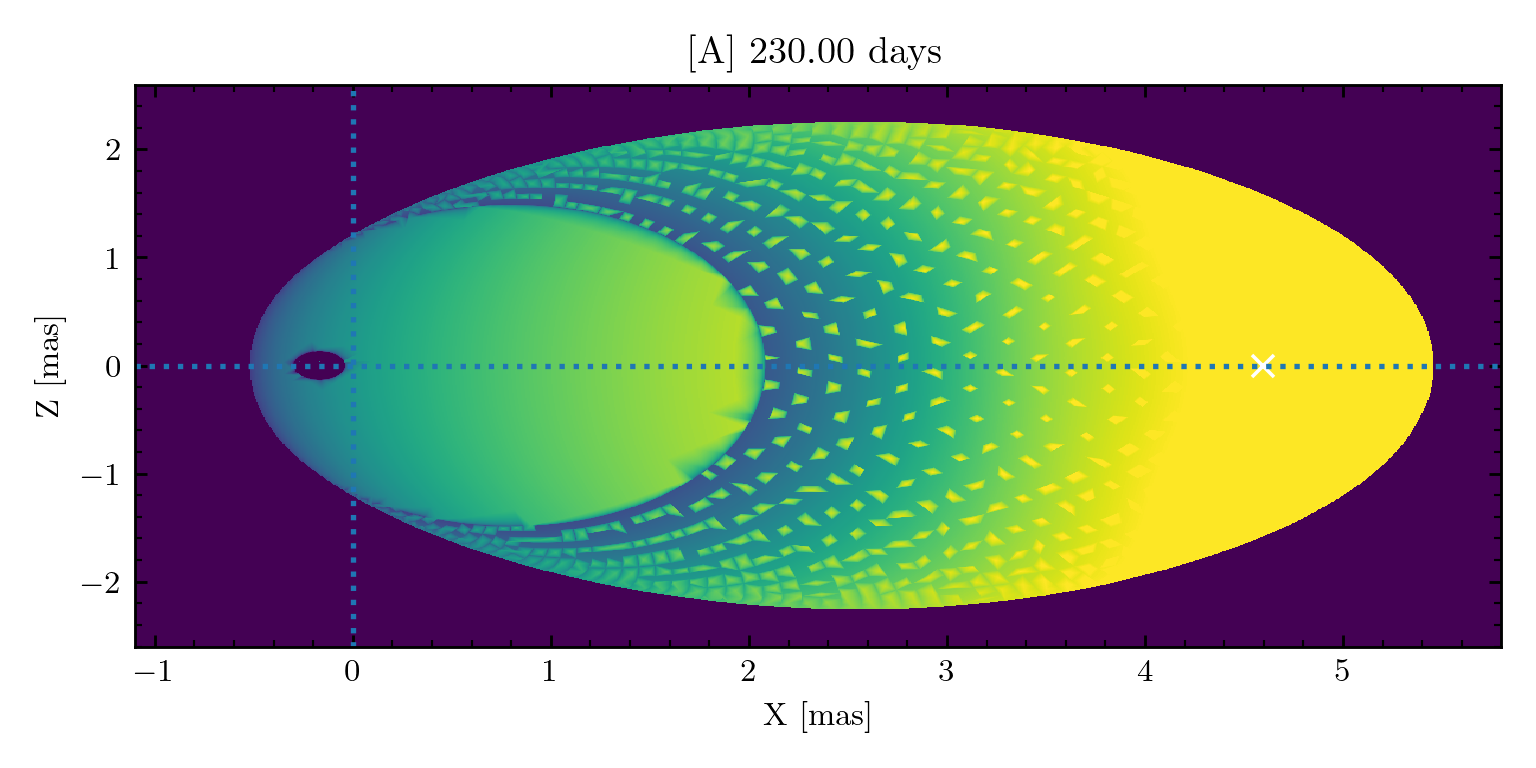
\includegraphics[height=4cm]{figures/plot_sky_image_jet.png}
            }};
        }
        \uncover<1->{ % <-> |
        \node (img1) [anchor=center,scale=1,opacity=1] at ([shift={(6.cm,-2.3cm)}]current page.center){
            \parbox{1.0\textwidth}{
                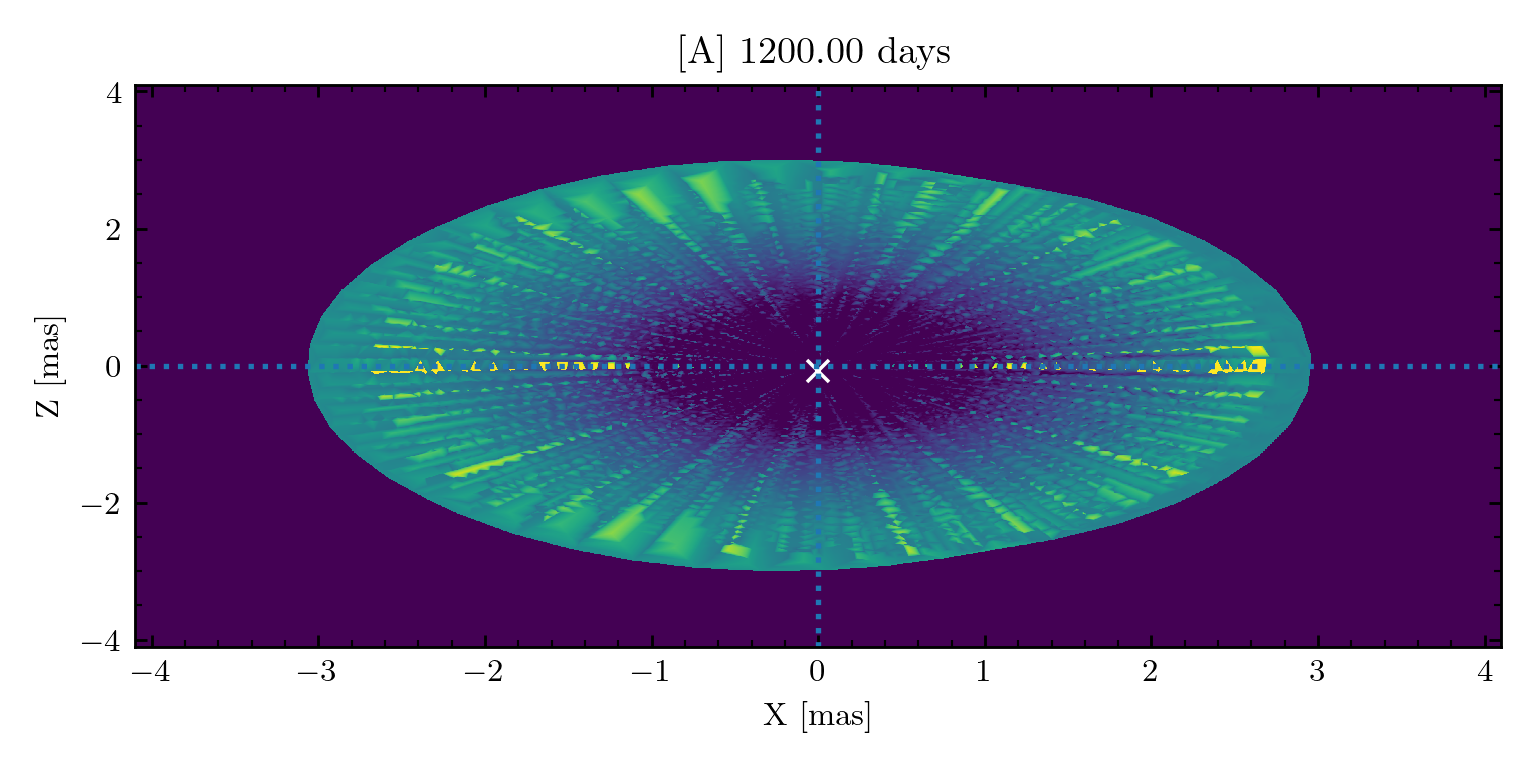
\includegraphics[height=4cm]{figures/plot_sky_image_ejecta.png}
        }};
        }
    \end{tikzpicture}
\end{frame}

%\section{Introduction}
%%% --------------------------------------------------------------
%%
%% I N T R O D U C T I O N
%%
%% --------------------------------------------------------------

\begin{frame}%{Binary neutron star (BNS) mergers}  %% ---------- Intro/motivation 

\begin{tikzpicture}[overlay,remember picture]

\uncover<1->{ % <-> |
    \node (t1) [anchor=center,scale=1,opacity=1] at ([shift={(-4.0cm,3.0cm)}]current page.center){
        \parbox{0.5\textwidth}{
        \begin{footnotesize}
            \textbf{Neutron stars (NSs)} are collapsed cores of massive stars, after core collapse supernovae
            % which had a total mass of between 10 and 25 solar masses
%            Unknown inner structure \\
%            If in binary, they will collide \\ 
        \end{footnotesize}
    }};
}
\uncover<1->{ % <-> |
    \node (t1) [anchor=center,scale=1,opacity=1] at ([shift={(-4.0cm,0.0cm)}]current page.center){
        \parbox{0.55\textwidth}{
            \textit{Binary neutron star (BNS) mergers} relate to
            \begin{itemize}
                \item origin of heaviest elements;
                \item origin of (some) short \acp{GRB};
                \item thoery of gravity;
                \item cosmology;
                %\item \nuc{} of the heaviest elements in the Universe,
                %\item cosmology.%, using \ac{BNS} mergers as standard sirens
            \end{itemize}
    }};
}
\uncover<1->{ % <-> |
    \node (t1) [anchor=center,scale=1,opacity=1] at ([shift={(-4.0cm,-3.0cm)}]current page.center){
        \parbox{0.55\textwidth}{
            \textit{Numerical relativity (NR) simulations} $\rightarrow$ 
            % \vspace{-5mm}
            \begin{itemize}
                \item \acp{GW} 
                \item ejecta properties 
            \end{itemize}
    }};
}
%\uncover<1->{ % <-> |
%    \node (t1) [anchor=center,scale=1,opacity=1] at ([shift={(-4.0cm,-2.0cm)}]current page.center){
%        \parbox{0.55\textwidth}{
%            \textbf{Multimessenger event}
%            \begin{itemize}
%                \item \GW{} (Gravitational waves)
%                \item \AT{} (kilonova)  %thermal electromagnetic (EM) emission, kilonova (kN), \AT{},
%                \item \GRB{} (short GRB)% non-thermal \ac{EM} short gamma-ray burst (GRB), \GRB{}
%            \end{itemize}
%            
%%            Wealth of information about different physical processes occurring in BNS\\
%            %\red{Questions}: remnant's lifetime; ejecta mass/composition; sources of \rproc{} elements
%    }};
%}

%\uncover<1->{ % <-> |
%    \node (t1) [anchor=center,scale=1,opacity=1] at ([shift={(0.0cm,-3.4cm)}]current page.center){
%        \parbox{1.1\textwidth}{
%%            \textcolor{black}{Major advanclemts} were maid in our understanding of related physical processes \\
%            \textcolor{black}{ \textbf{Key questions}}: remnant fate; origin of the early kilonova emission; origin of the late \ac{GRB} afterglow; \\
%            \textbf{What is NS equation of state (\ac{EOS})?}
%    }};
%}

\uncover<1->{ % <-> |
    \node (img1) [anchor=center,scale=1,opacity=1] at ([shift={(3.4cm,-0.2cm)}]current page.center){
        \parbox{0.5\textwidth}{
            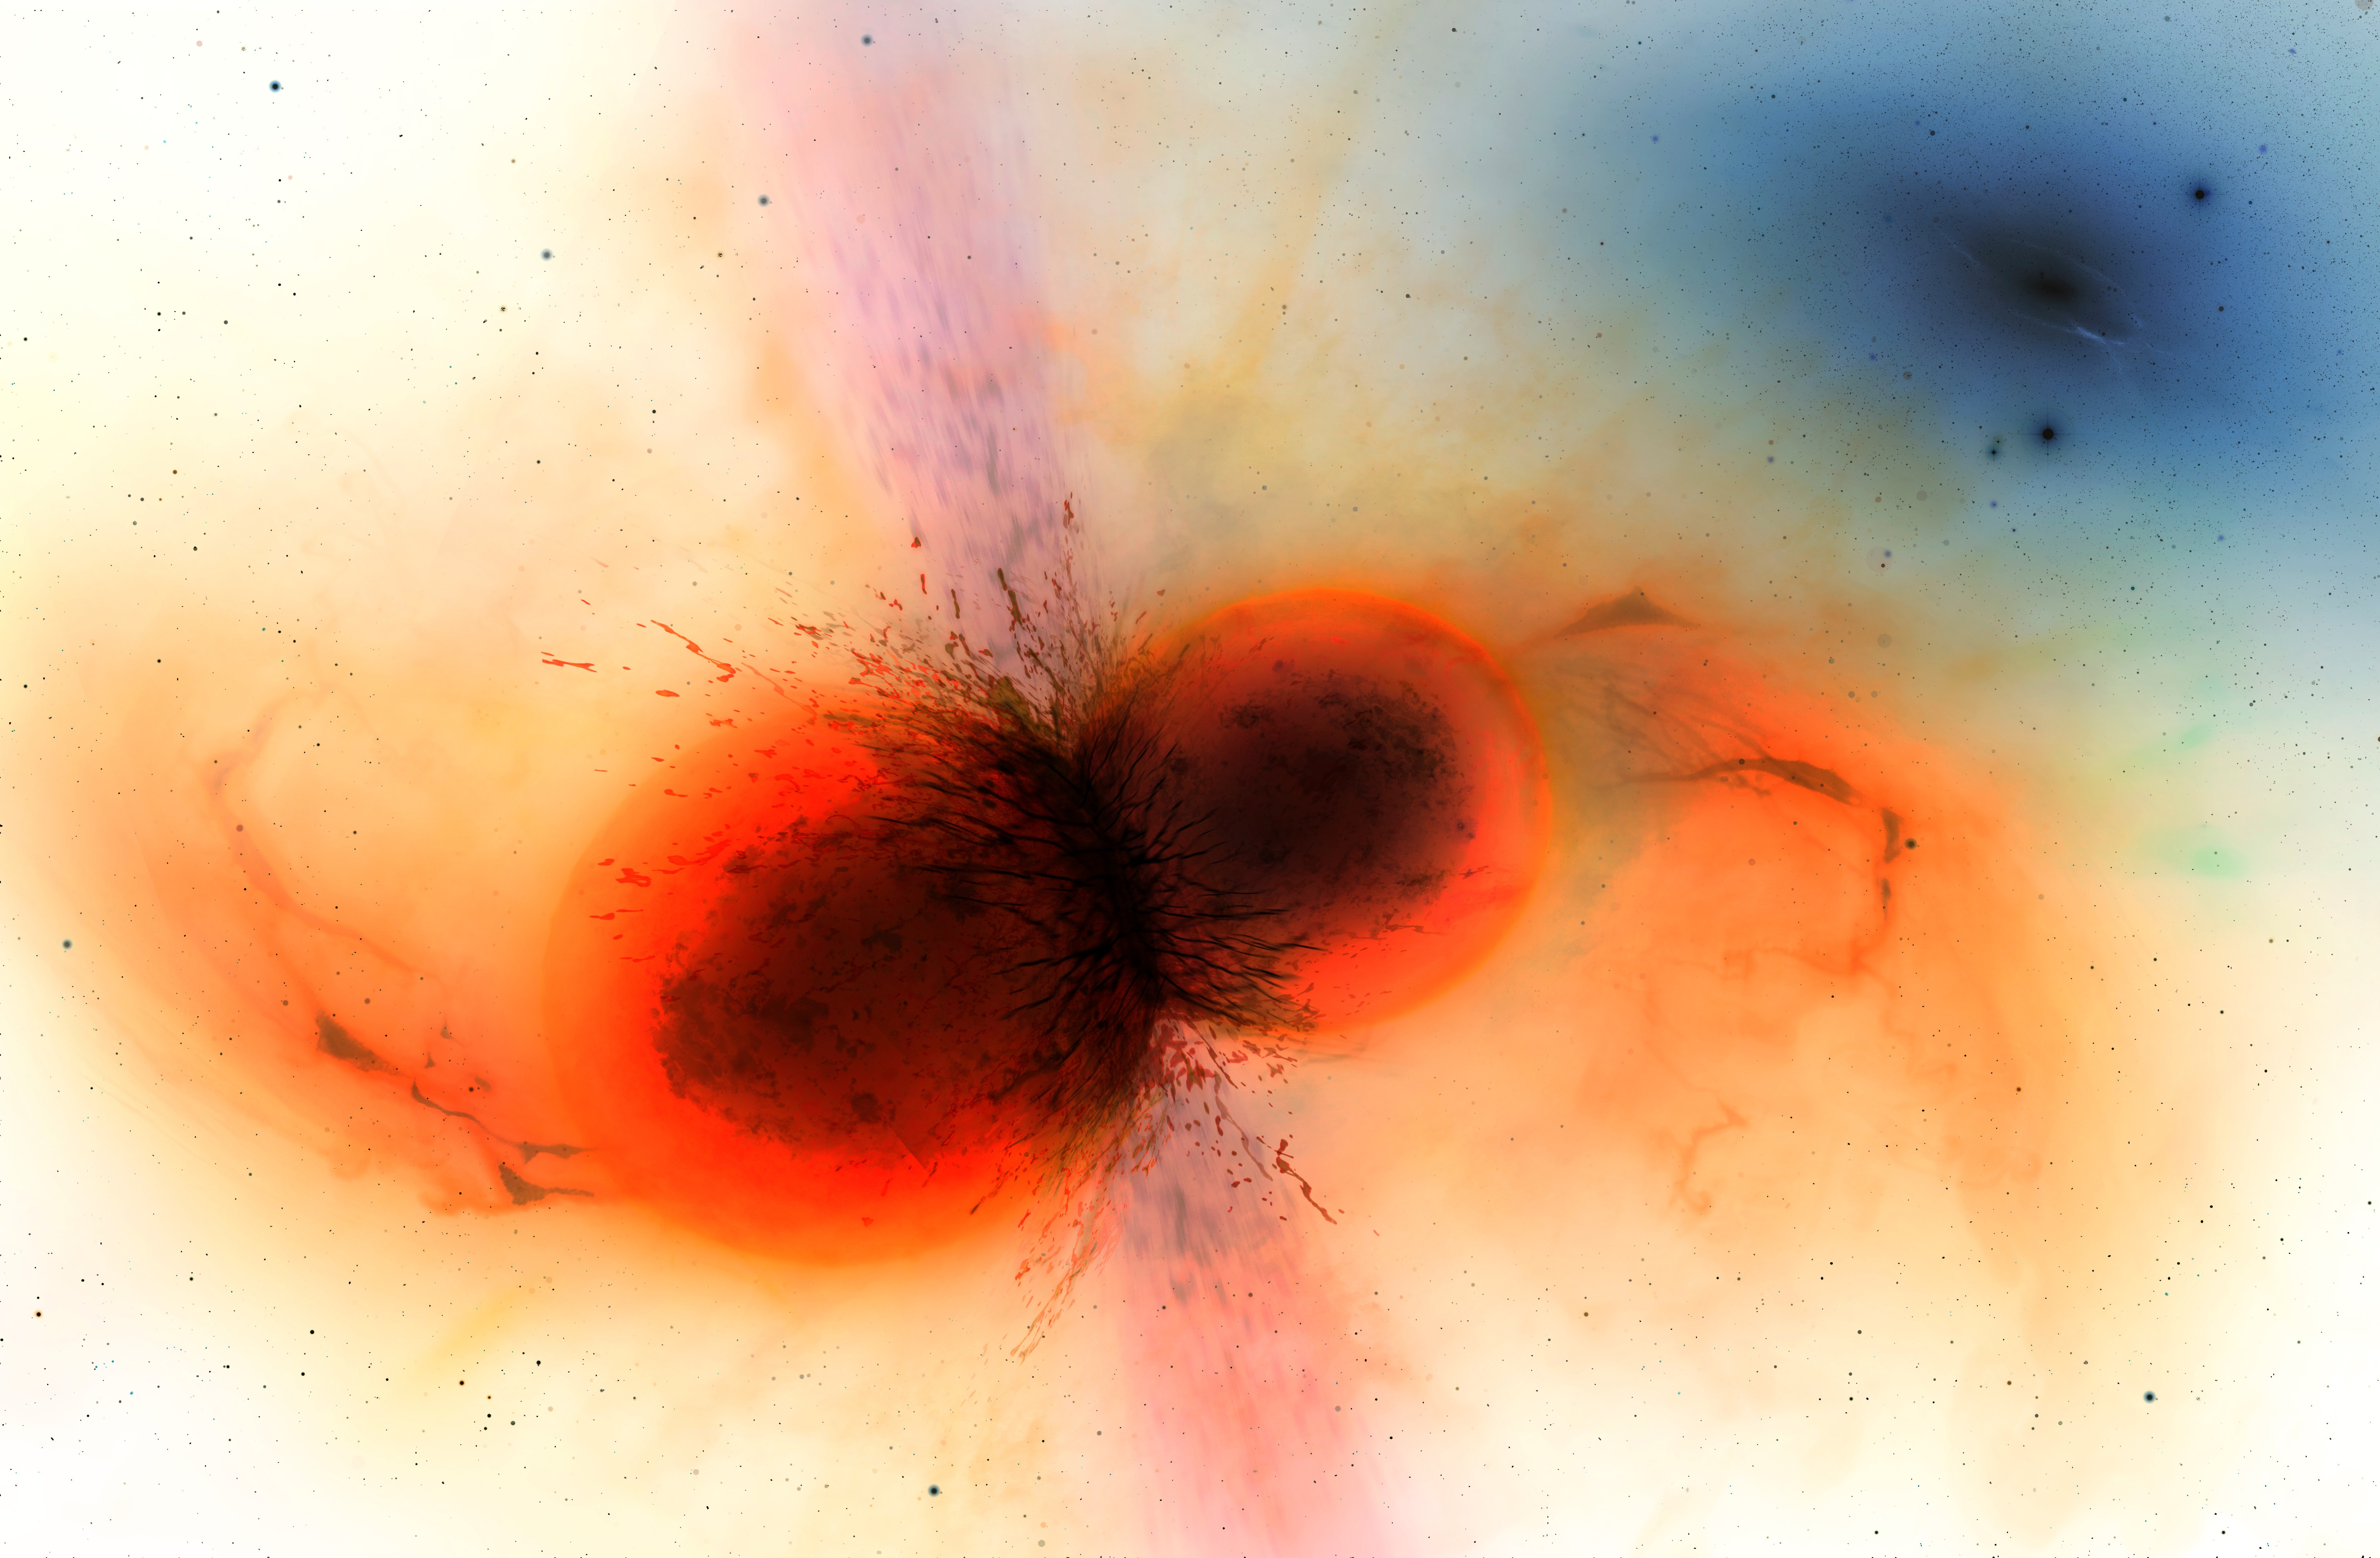
\includegraphics[height=5.3cm]{figures/bns_cartoon_inveted.jpg}\\
            Artist depiction of merging neutron stars \\
            \textcolor{gray}{ \footnotesize{
                    Credit: University of Warwick/Mark Garlick} 
                }
    }};
}


\end{tikzpicture}
\end{frame}

%% ----------------------------------------------------------------------------------

\begin{frame}%{Binary neutron star (BNS) mergers}  %% ---------- Intro/motivation 
    
    \begin{tikzpicture}[overlay,remember picture]
        \uncover<1->{ % <-> |
            \node (t1) [anchor=center,scale=1,opacity=1] at ([shift={(-3.6cm,2.0cm)}]current page.center){
                \parbox{0.60\textwidth}{
                    August 2017 \textbf{Multimessenger event}
                    \begin{itemize}
                        \item \GW{} -- \ac{GW}
                        \item \AT{} -- thermal \ac{EM} emission, kilonova (kN)  %thermal electromagnetic (EM) emission, kilonova (kN), \AT{},
                        \item \GRB{} -- non-thermal \ac{EM} short \ac{GRB}% non-thermal \ac{EM} short gamma-ray burst (GRB), \GRB{}
                    \end{itemize}
                    
                    %            Wealth of information about different physical processes occurring in BNS\\
                    %\red{Questions}: remnant's lifetime; ejecta mass/composition; sources of \rproc{} elements
            }};
        }
        
        \uncover<1->{ % <-> |
            \node (t1) [anchor=center,scale=1,opacity=1] at ([shift={(-3.6cm,0.0cm)}]current page.center){
                \parbox{0.60\textwidth}{
                     \textit{\ac{EM} models} $\rightarrow$ ejecta properties.
            }};
        }
    
        \uncover<1->{ % <-> |
            \node (t1) [anchor=center,scale=1,opacity=1] at ([shift={(-3.6cm,-2.0cm)}]current page.center){
                \parbox{0.60\textwidth}{
                    \textbf{Question:}\\
                    Binary parameters and \ac{NS} \ac{EOS}?
                    %by using \ac{NR} simulations and \ac{EM} counterparts 
            }};
        }
    
%        \uncover<1->{ % <-> |
%            \node (t1) [anchor=center,scale=1,opacity=1] at ([shift={(0.0cm,-3.4cm)}]current page.center){                    Artist depiction of merging neutron stars \\
%                \textcolor{gray}{ \footnotesize{
%                        Credit: University of Warwick/Mark Garlick} 
%                }
%                \parbox{1.1\textwidth}{
%                    %            \textcolor{black}{Major advanclemts} were maid in our understanding of related physical processes \\
%                    \textcolor{black}{ \textbf{Key questions}}: remnant fate; origin of the early kilonova emission; origin of the late \ac{GRB} afterglow; \\
%                    \textbf{What is NS equation of state (\ac{EOS})?}
%            }};
%        }
        
        \uncover<1->{ % <-> |
            \node (img1) [anchor=center,scale=1,opacity=1] at ([shift={(5.cm,0.0cm)}]current page.center){
                \parbox{0.4\textwidth}{
                    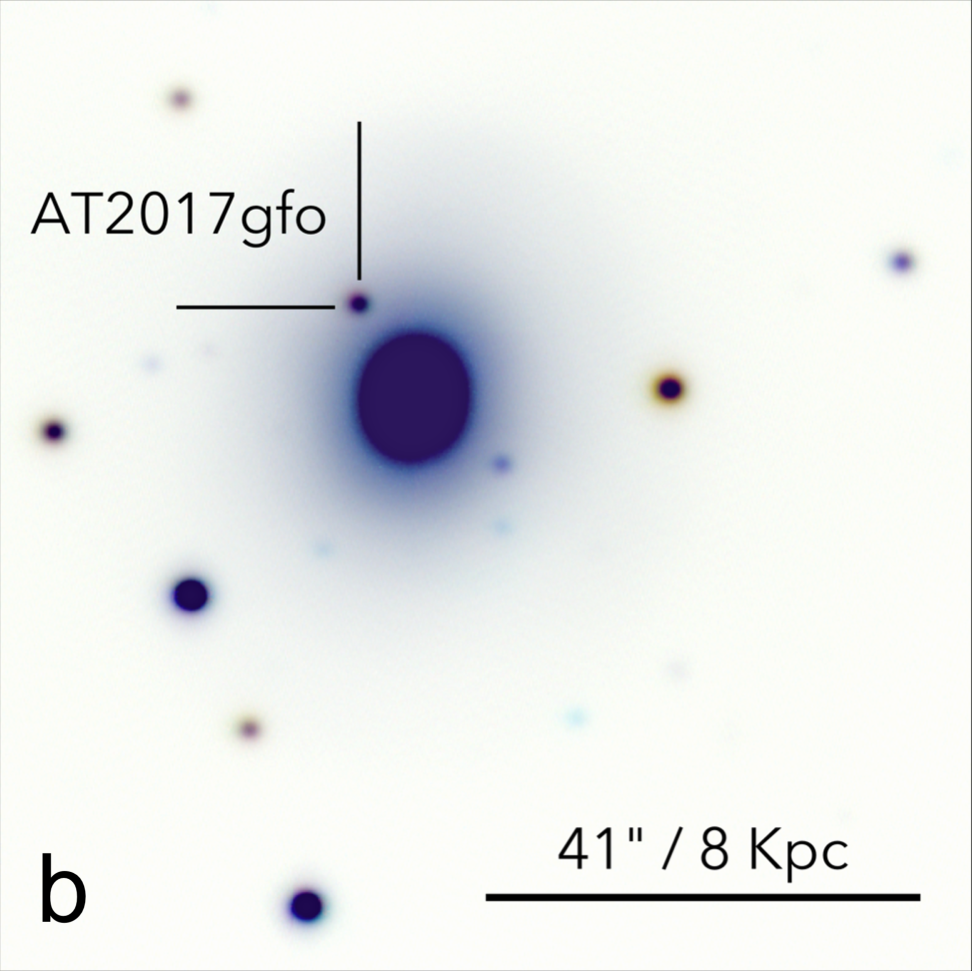
\includegraphics[height=5.3cm]{figures/at2017gfo_smartt_inv.png}\\
                    Image of AT2017gfo\footcite{Smartt:2017fuw}
                    %$^{\textcolor{gray}{\text{\cite{Smartt:2017fuw}}}}$
            }};
        }
        
    \end{tikzpicture}
\end{frame}
%\section{Simulations}
%%% --------------------------------------------------------------
%%
%% N R  S I M U L A T I O N S
%%
%% --------------------------------------------------------------
\begin{frame}{Method} %% ---------- title 
\begin{tikzpicture}[overlay,remember picture]
\uncover<1->{ % <-> |
    \node (t1) [anchor=center,scale=1,opacity=1] at ([shift={(-0.0cm,-0.2cm)}]current page.center){
        \parbox{1.1\textwidth}{
            Key physics: General Relativity, fluid dynamics, radiation transport. 
            \begin{equation*}
                R_{\mu\nu}-\frac{1}{2}Rg_{\mu\nu}=8\pi T_{\mu\nu}, \hspace{5mm} \nabla_{\mu}T^{\mu\nu} = 0, \hspace{5mm} \frac{DF}{Dl}=\mathcal{C}[F]
            \end{equation*}
            %
            Complex numerical implementation. Expensive simulations. \\
            Numerical relativity codes, \eg, \wisky{} code$^\text{\citep{Radice:2013apa,Radice:2012cu,Radice:2013xpa,Radice:2013hxh,
                                 Radice:2015nva,Radice:2016dwd,Radice:2018pdn,Radice:2020ids}}$
            \begin{itemize}
                \item Z4c formulation of $3+1$ decomposed, general relativity,
                %\item Conservative formualtion of relativistic hydrodynamics,
                \item Neutrino radiation transport via Leakage $+$ M0 scheme,
                \item Turbulent viscosity of magnetic origin via GRLES appraoch,
                \item Microphsyical EOS with finite temperature effects.
            \end{itemize}
            Overall, $37$ unique simulations targeted to \GW{}, (some $100+$~ms) % total of $76$,  \\
            % Initial data: constraint equations + Helical killing vector + conformal flatness
            % For free evolution we use z4c: conformal decomposition of the metric fields with improved constraint propagation + dampening (better for non-vacuum spacte time)
            % Moving-puncture gauge (1+log and Gamma-driver) to deal with forming BHs and moving pucntures
            % GRHD is in the conservative formulation, with central, HRSC scheme.
            % Neutrinos are treated with moment formalism, where moment representaiton of Boltzman equation, truncated at (M1 - 2nd moment) with closure achieved via interpolation between otpically thin and thick regimes. 
            % LEackages scheme is na approximation to transport equations that concerns only with the change in leptonic number and loss of energy (no momentum transport or diffusion)
            % EOS: Skyrme model with finite-temperature and composition dependencies (LS220 SLy4) 
            %      Rel.Mean.Field with -//- (DD2 SFh0)
            %      Brueckner-Hartree-Fock extensitions to finite.temp. (BLh)
            % SOftening at very high rho - Lambda-Hyperons or phase transition
            % Numerically: evolution is performed with method of lines and BErger-Oliger algorithm with sub-cycling in time and refluxing 
    }};
}
%
%\uncover<2->{ % <-> |
%    \node (t1) [anchor=center,scale=1,opacity=1] at ([shift={(-0.0cm,-3.6cm)}]current page.center){
%        \parbox{1.1\textwidth}{
%            \textbf{Goal}: Analyzed ejecta/\nuc{}/EM counterparts \& statistical analysis \\
%            \textbf{Methods}: Post-processing pipeline \texttt{bns\_ppr\_tools} for ejecta/disk/remnant
%%            \begin{itemize}
%%            \item Developped post-processing pipeline \texttt{bns\_ppr\_tools}
%%            \item \textbf{Goal}: Analyzed for ejecta/\nuc{}/EM counterparts \& statistical analysis
%%%            \item Statisitcal analysis alongside other models in literature
%%            \end{itemize}
%    }};
%}
\end{tikzpicture}
\end{frame}

%% ----------------------------------------------------------------------------

\begin{frame}{Representative picture of a binary neutron star merger} %% ---------- title 
\begin{tikzpicture}[overlay,remember picture]
    \uncover<1->{ % <-> |
    \node (t1) [anchor=center,scale=1,opacity=1] at ([shift={(-4.1cm,0.5cm)}]current page.center){
        \parbox{0.50\textwidth}{
            
            % Inspiral (${\simeq}10\,$orbits); NSs Zero-temperature, $\beta$-equilibrium \\
            % Merger \& post-merger, $T{\sim}50\,$MeV, $\rho{\sim3.6}\rho_0$. \\
            % Postmerger: Remnant $+$ disk $+$ ejecta; \\
            % Fate: $J$ transport; MHD; $\nu$, GWs \\
            \textbf{System parametrization:} \\
            Tidal interaction 
            % Distrortion of the mass distribution of a given NS in a Grav. Field of another
            % Parametrized with Love Number (computed by solving perturbation of a relativistic star k=f(EOS,Compactness))
            % Combining compactness and Love we get tidal polarizability parameter
            % The dynamics of the two bodies can be described with tidal coupling constant that 
            % describes tidal interaction at leading order
            % Tidal interaction (i) attractive (ii) short range: They accelerate merger, increase frequency
            can be parameterized with \textit{reduced tidal parameter}
            %
            \begin{equation*}
                \tilde{\Lambda} := \frac{16}{13}\frac{(M_A + 12M_B)M_A^4}{M^5}+(A\leftrightarrow B)
            \end{equation*}
            % Gravitational massess are estimated in (conformal, assymptitic? flatness?) in far-field regime and are estimated as integrals over fluid configuration
            %
            $\downarrow\tilde{\Lambda}$ for softer EOS, $\uparrow M$, $\uparrow q=M_A/M_B$ \\
            %
            % A moment of merger is a maximum of the GW amplitude
            %
            % Gauge invariant quantities: Reduced binding energy and angular momentum
            % During the evolution they decrease as GW carry energy away
            % Quasiuniversality: EOS can be captured with $\tilde{\Lambda}$ for equal mass binary
        
    }};
    }
%
    \uncover<1->{ % <-> |
    \node (t1) [anchor=center,scale=1,opacity=1] at ([shift={(3.6cm,0.8cm)}]current page.center){
        \parbox{0.55\textwidth}{
            \textbf{Post-merger state:} \\
            BH, long/short-lived remnants, and disks \\
            % Early postmerger: 
            Core bounces: cold inside, hot interface; shocks at NS surface only \\
            % Neutrino burst, ${\sim}15\,$MeV. 
            % Neutrino decouple at different radii
            % Abundance of free $n$, absorbe $\nu_e$, raise $Y_e$; emission of $\bar{\nu}_e$
            % Possible phase transition softens EOS
            % Impact of phase transition depends on density at which it occure
            While cores fuse, remnant shows bar-like deformation \\
            % Main post-merger GW freq. = 2 times dynamical freq.
            % Peaks in GWs associated with hydro mode 
            % Peak frequencies depend on NS prop. -- quasiuniversality
            % Ang. Mom. at merger determines the angular vel. of the bulk of matter
            % Most luminous $\neq$ largest energy
            % Simulations give upper limitof GWs energy
            % GWs backreacts on the fluid, damping the non-axisymmetric modes
            Remnant evolves towards axisymmetry \\
            % Postmerger state: super-Keplerian $J>J_{\rm max}^{\rm equilib}$, $M_b>M_{b \rm, max}^{\rm eqilib}$
            % Thermal and neutrino effects $\uparrow$ pressure (${\simeq}10\%$), hence, radius, but not the $M_{\rm max}$. 
            % Rotatin increases NS $M_{\rm max}$ and $R$. 
            % Note: In postmerger $M_{\rm max}^{\rm hot} < M_{\rm max}^{\rm cold}$
            % hence, temperature effects do not stabilize the star.
            % Larger radiuss $\rightarrow$ lower mass-shedding limit
            % Overall: cold classification do not (SMNS, HMNS...) do not apply
            % Magnetic fields can raise $M_{\rm max}$, affecting angular momentum distribution
            % Angular momentum redistribution occures on a viscous time-scale.
            % Inclusion of viscosity show shorter collapse time. 
            % Simulations show a ritational profile with a minimum at the core; as viscous and hydro effects counteract Grav. instabilities in the core, the core will spin up, compactness reduces, hence, the core must shed the excess in angular momentum. Through winds!
            % Neutrinos primarely cool the remnant, removing some of the excess in binding energy. 
            % Simulations show that one-armed instability persists on ${\sim}50\,$ms timescale.
            % Disk $\rho < 10^{13}\,$\gcm
            % Volume integral of the conserved rest-mass density
            % Properties depend on formation
            % formed from matter expelled by tidal torquies at merger 
            % Structure: coled tidal component $+$ hot shocked
            % Nass of the disk may rise as $M_b$ and $J$ are shed by the remnant
            % Shocks ($m=1$) raise entropy, Keplerian, temp profile $\{10,0.1\}$MeV
            % BH formation removes ${\sim}50$ disk
            % Disks around BHs are more compact and hotter
            % In case of PC, $q=1$ binaries give little disk, while $q{\simeq}1.4$ result in more massive disks. Hiher $q$ lead to tidal disruption of a compantion and formation of a massive cold disk.
            % In high $q$ cases tidal tail falls back, disturbing the disk
    }};
    }

    \uncover<1->{ % <-> |
        \node (img1) [anchor=center,scale=1,opacity=1] at ([shift={(-1.cm,-2.8cm)}]current page.center){
            \parbox{1.0\textwidth}{
                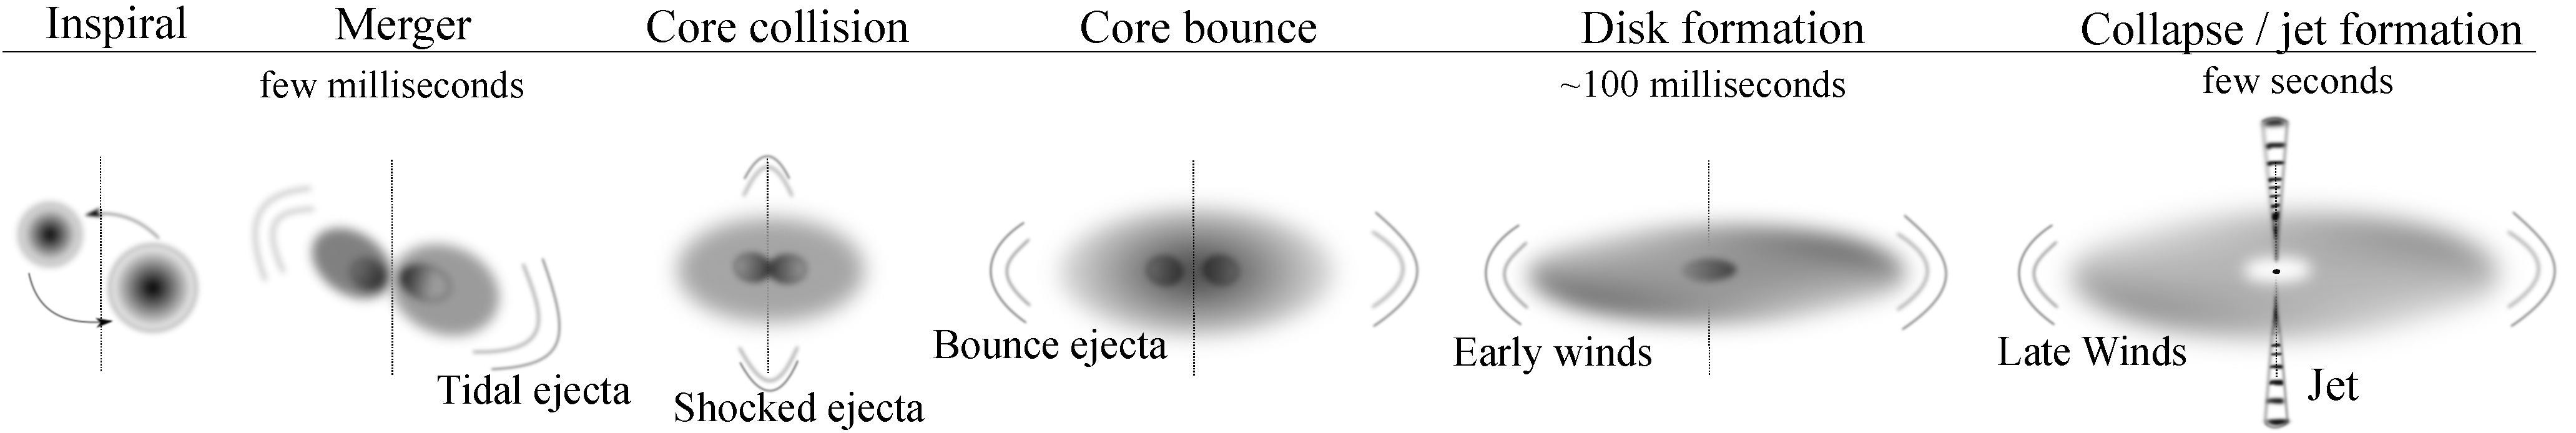
\includegraphics[height=2.7cm]{figures/bns_evolution_transparent.pdf}
                %            \hspace*{10mm} Density modes in the remnant 
                %Modes analysis for exemplary equal-mass long-live and short-lived
                %        remnants. The evolution of the $m=2$ and the $m=1$ monitored by
                %        Eq.~\eqref{eq:modes} is shown for the DD2 and LS220 remnant with and
                %        without turbulent viscosity. The $m=2$ mode in the long-lived
                %        remnant is strongly damped by the emission of gravitational
                %        radiation and becomes comparable to the $m=1$ mode on a timescale of
                %        ${\gtrsim}20\,$ms. Turbulent viscosity sustain the $m=2$ mode for
                %        a longer period. The $m=2$ mode is instead dominant to collapse in
                %        the short-lived remnant.
                %        (Adopted from \cite{Nedora:2020pak})
        }};
    }
\end{tikzpicture}
\end{frame}
%% ----------------------------------------------------------------------------

\begin{frame}{Hydrodynamic modes in the \pmerg{} remnant$^\text{\citep{Nedora:2019jhl,Nedora:2020pak}}$} %% ---------- title 
    
    \begin{tikzpicture}[overlay,remember picture]
        
        \uncover<1->{ % <-> |
            \node (t1) [anchor=center,scale=1,opacity=1] at ([shift={(-3.6cm,1.5cm)}]current page.center){
                \parbox{0.6\textwidth}{
                    Decomposition in Fourier modes $e^{-i m\phi}$ 
                    of the Eulerian rest-mass density 
                    \begin{equation*}
                        \label{eq:modes}
                        C_m(t) = \int \rho(x,y,z=0,t) e^{-i m \phi(x,y)} \text{d}x \text{d} y \, ,
                    \end{equation*}
            }};
        }
        %
        \uncover<1->{ % <-> |
            \node (img1) [anchor=center,scale=1,opacity=1] at ([shift={(4.5cm,-0.6cm)}]current page.center){
                \parbox{0.5\textwidth}{
                    \includegraphics[height=6.4cm]{phd_figs/remnant/dens_modes/modes_rho_dd2.pdf}
                    \hspace*{10mm} Density modes in the remnant 
                    %Modes analysis for exemplary equal-mass long-live and short-lived
                    %        remnants. The evolution of the $m=2$ and the $m=1$ monitored by
                    %        Eq.~\eqref{eq:modes} is shown for the DD2 and LS220 remnant with and
                    %        without turbulent viscosity. The $m=2$ mode in the long-lived
                    %        remnant is strongly damped by the emission of gravitational
                    %        radiation and becomes comparable to the $m=1$ mode on a timescale of
                    %        ${\gtrsim}20\,$ms. Turbulent viscosity sustain the $m=2$ mode for
                    %        a longer period. The $m=2$ mode is instead dominant to collapse in
                    %        the short-lived remnant.
                    %        (Adopted from \cite{Nedora:2020pak})
            }};
        }
        
        \uncover<1->{ % <-> |
            \node (t2) [anchor=center,scale=1,opacity=1] at ([shift={(-3.8cm,-1.8cm)}]current page.center){
                \parbox{0.6\textwidth}{
                    \begin{itemize}
                        \item Newly born remnant is not axisymmetric
                        \item Bar-shaped $m=2$ dominats the \textbf{early} phase
                        and later $m=2$ is damped by the emission of \acp{GW}
                        \item One-armed $m=1$ is present on ${\sim}100$~ms 
                        \item $m=1$ mode is stronger if \mr{} is higher
                        \item And as the $m=1$ modes are not efficiently damped$^\text{\citep{Paschalidis:2015mla,Radice:2016gym,Lehner:2016wjg,East:2016zvv}}$
                    \end{itemize}
            }};
        }

\end{tikzpicture}
%\begin{itemize}
%    \item Not axisymmetric. Angular momentum redistribution, \acp{GW} losses %\cite{Bernuzzi:2015opx,Radice:2018xqa}
%    \item Long-term evolution driven by viscous processes \& weak interactions
%    \item After \ac{GW} losses \ac{MNS} have excess in $M$ with respect to the cold, rigid.rot equilibria %\citep{Radice:2018xqa}.
%    \item \ac{MNS} remnant evolves towards stability at the mass-shedding limit
%    \item Collapse to a \ac{BH} depends on post-merger state, temperature and composition
%\end{itemize}
%
%\begin{figure}[t]
%    \centering
%    \includegraphics[width=0.49\textwidth]{raycasting_smooth_cropped.pdf}
%    \caption{3D distribution of angular momentum density flux $J_r$
%        from the DD2 simulation with turbulent viscosity at ${\sim}43.5$~ms after
%        merger. $J_r$ is shown on a central region of
%        $(89\times89\times60)$~km${}^3$ covering the remnant NS
%        and disk, and it is given in units where $c=G=\Msun=1$.
%        (Adapted from \citet{Nedora:2019jhl})
%    }
%    \label{fig:ang_mom_flux}
%\end{figure}
%
%\begin{itemize}
%    \item High $q$ models undergo prompt collapse (no core bounce) % central density monotonically rises\citep{Radice:2020ddv,Bernuzzi:2020tgt,Bernuzzi:2020txg}. 
%    \item 
%\end{itemize}
\end{frame}

%% ----------------------------------------

%% FROM LETTER 

%From the fluid's stress energy tensor,
%we compute the angular momentum density flux $J_r = T_{ra}(\partial_\phi)^a$,
%where $\phi$ is the cylindrical angular coordinate;
%angular momentum is conserved if $(\partial_\phi)^a$ is a Killing vector.
%
%% FROM PAPER 

%The fluid's angular momentum analysis in the remnant and disk is performed
%assuming axisymmetry,
%%(see Appendix~\ref{app:ang} for derivation)
%that is, we assume $\phi^{\mu} = (\partial_{\phi})^{\mu}$ is a Killing
%vector. Accordingly, the conservation law (Eq.~\eqref{eq:theory:tmunu_eq_0}) 
%reads
%%
%\begin{equation}
%\partial_t(T^{\mu\nu}\phi_{\nu}n_{\nu}\sqrt{\gamma}) -
%\partial_i(\alpha T^{i \nu}\phi_{\nu}\sqrt{\gamma}) = 0 \ ,
%\end{equation}
%%
%where $n^\mu$ is the normal vector to the spacelike hypersurfaces of
%the spacetime's $3+1$ decomposition.
%%
%The equation implies the conservation of the angular momentum 
%\begin{equation}
%J = % \int j dV = 
%%- \int \, T_{\mu\nu}n^{\mu}\phi^{\nu}\,\dd ^3x = 
%-\int \,
%T_{\mu\nu}n^{\mu}\phi^{\nu}\,\sqrt{\gamma}\, \dd^3 x\ .
%\end{equation}
%%
%In the cylindrical coordinates $x^i=(r,\phi,z)$ adapted to the symmetry
%the angular momentum density is  
%%
%\begin{equation}
%j = %-
%\rho h W^2 v_{\phi} \ ,
%\label{eq:method:ang_mom}
%\end{equation}
%%
%and the angular momentum flux is 
%%
%\begin{equation}
%\alpha\sqrt{\gamma}T^r _{\nu}\phi^{\nu} =
%\alpha\sqrt{\gamma}\rho h W^2 (v^{r}v_{\phi}) .
%\end{equation}
%
%We evaluate these quantities from the 3D snapshots of our simulations.


%% ----------------------------------------------------------------
%%
%% Spiral Arms
%%
%% ----------------------------------------------------------------

\begin{frame}{Spiral arms in \pmerg{} remnant$^\text{\citep{Nedora:2019jhl}}$} %% ---------- title 
\begin{tikzpicture}[overlay,remember picture]
\uncover<1->{ % <-> |
    \node (t1) [anchor=center,scale=1,opacity=1] at ([shift={(-3.2cm,1.2cm)}]current page.center){
        \parbox{0.65\textwidth}{
            The angular momentum flux in the cylindrical coordinates.% $x^i=(r,\phi,z)$.
            % $\phi^{\nu}$ is the generator of the rotations in the orbital plane.
            \begin{equation*}
            \alpha\sqrt{\gamma}T^r _{\nu}\phi^{\nu} =
            \alpha\sqrt{\gamma}\rho h W^2 (v^{r}v_{\phi})\, ,
            \end{equation*}
            assiming $\phi^{\mu} = (\partial_{\phi})^{\mu}$ is a Killing vector. % angular momentum is conserved
    }};
}

\uncover<1-1>{ % <-> |
    \node (img1) [anchor=center,scale=1,opacity=1] at ([shift={(5.3cm,-0.6cm)}]current page.center){
        \parbox{0.5\textwidth}{
            \includegraphics[height=6cm]{phd_figs/raycasting_smooth_cropped.pdf}
            
            \hspace*{2.8mm}Spiral arms within the disk
    }};
}

%shocks are generated at the collisional interface of the \acp{NS} cores,
%as well as, tidal torques exerted by the non axisymmetric remnant result in a formation
%of the disk.
%Matter, energy and angular momentum are injected into the disk as the spiral 
%density waves propagate outwards from the mass-shedding \ac{MNS} remnant
\uncover<1->{ % <-> |
    \node (t2) [anchor=center,scale=1,opacity=1] at ([shift={(-3.5cm,-1.8cm)}]current page.center){
        \parbox{0.6\textwidth}{
            \begin{itemize}
                \item Shocks and tidal torques exerted from non-axisymmetric remnant $\rightarrow$ disk;
                \item spiral arms is a generic hydrodynamic effect.
            \end{itemize}
            Injection of matter, energy and angular momentum.
    }};
}

\end{tikzpicture}

\end{frame}


%% ----------------------------------------------------------------
%%
%% Angular momentum trasport
%%
%% ----------------------------------------------------------------

\begin{frame}{Angular momentum transport in \pmerg{} remnant$^\text{\citep{Nedora:2020pak}}$} %% ---------- title 

\begin{tikzpicture}[overlay,remember picture]

\uncover<1->{ % <-> |
    \node (img2) [anchor=center,scale=1,opacity=1] at ([shift={(4.2cm,-0.4cm)}]current page.center){
        \parbox{0.5\textwidth}{
            \includegraphics[height=6.0cm]{phd_figs/remnant/evol_jflux_2d_DD2_M13641364_M0_SR_R1.pdf}
            
            \hspace*{2.8mm}Ang. mom. transport through disk
    }};
}
%shocks are generated at the collisional interface of the \acp{NS} cores,
%as well as, tidal torques exerted by the non axisymmetric remnant result in a formation
%of the disk.
%Matter, energy and angular momentum are injected into the disk as the spiral 
%density waves propagate outwards from the mass-shedding \ac{MNS} remnant

\uncover<1->{ % <-> |
    \node (t2) [anchor=center,scale=1,opacity=1] at ([shift={(-3.8cm,-0.8cm)}]current page.center){
        \parbox{0.6\textwidth}{
            \begin{itemize}
                \item The $J$ is transported via spiral waves induced by $m=\{1,2\}$ modes.
                \item Spiral density modes inject ${\sim}0.1-0.4\,\Msun$ into the disk
                \item ${\sim}50\%$ of $J$ remnant $\rightarrow$ disk
                \item Mass injection is stronger in models with stiffer EOS. 
                \item Accretion, mass-shedding, weak processes
                \item Larger temperatures lead to lower rotational frequency at which the mass 
                shedding occurs% \citep{Kaplan:2013wra}. 
            \end{itemize}
    }};
}

\end{tikzpicture}

\end{frame}



%% ----------------------------------------------------------------
%%
%% Long-term Evolution
%%
%% ----------------------------------------------------------------



\begin{frame}{Long term evolution \& remnant's fate$^\text{\citep{Nedora:2020pak}}$} %% ---------- title 

%As the disk expands and cools, the recombination of nucleons into alpha particles 
%starts to take place. The energy, released in recombination, might be sufficient 
%for the outermost layers to become unbound, generating an outflow and contributing 
%to the disk depletion \citep{Beloborodov:2008nx,Lee:2009uc,Fernandez:2013tya}.
%%
%This process however is expected to take place on timescales, longer than
%those that are simulated here. On the $\sim100$~ms timescale, however, the outflows 
%are driven by the neutrino heating, above the remnant, the so-called neutrino-driven 
%wind (\nwind; \citep{Dessart:2008zd,Perego:2014fma,Just:2014fka}), and by the dynamical 
%interactions between the \ac{MNS} remnant and the disk, the \swind{} \citep{Nedora:2019jhl}.
%%
%We discuss the properties of the \nwind{} found in our simulations
%in Sec.~\ref{sec:bns_sims:nwind} and the properties of the 
%\swind{} in Sec.~\ref{sec:bns_sims:sww}.

\begin{tikzpicture}[overlay,remember picture]

%We evaluate the amount of angular momentum lost to \acp{GW} following the 
%\citet{Damour:2011fu,Bernuzzi:2012ci,Bernuzzi:2015rla}\footnote{
%    The radiated angular momentum is computed from the 
%    multipole loments $N_{lm}$ for the \ac{NR} complex "news function" at infinity. 
%    The $J_{z;\text{rad}}(t)$ is computed as \citep{Damour:2011fu} 
%    \begin{equation*}
%    \Delta J_{z\text{rad}}(t) \frac{1}{16}\sum_{l,m}^{l_{max}}\int_{t_0}^{t} dt' m \mathcal{L}[h_{lm}(t')(N_{lm}(t'))^*],
%    \end{equation*}
%    where $h_{lm}$ is the multipolar metric waveform, 
%    $N_{lm}(t) = dh_{lm}(t) / dt$, the news function, and $l_{max}=8$.
%    The $J$ loss is metric dependent ($h$).
%    The $h$ (strain???) is computed from $\Psi_4(t) = dN/dt = d^2h/dt^2$ by a 
%    frequency-domain integration procedure with a low-frequency cut 
%    $\omega_0 = 0.032/(m_1+m_2)$.
%    The routines used for the calculation are taken from the scientific library
%    \texttt{scidata}, available at \url{https://bitbucket.org/dradice/scidata}.
%}.

\uncover<1->{ % <-> |
    \node (t1) [anchor=center,scale=1,opacity=1] at ([shift={(-3.1cm,0.5cm)}]current page.center){
        \parbox{0.7\textwidth}{
            \begin{itemize}
                % Viscosity foces rotating equilibria to rotate rigidly
                % Non-axial symmetry -- gravitational radiation
                \item Remnant borm with excess in $M_b$ and $J$ (HMNS)
                \item GWs remove some $J$
                \item Massive outflows from expanded disk
                driven by $m=\{1,2\}$ and $J$ transport
                \item \swind{} Removes $J$ and $M_b$
                \item The remannt can reach stable configuration
                \item Study of remnant's fate requries long 3D NR simulations
            \end{itemize}
    }};
}

\uncover<1->{ % <-> |
    \node (img1) [anchor=center,scale=1,opacity=1] at ([shift={(4.6cm,-0.2cm)}]current page.center){
        \parbox{0.5\textwidth}{
            \includegraphics[height=6cm]{phd_figs/ejecta_sec/secular_j_mb_RNS_blh.pdf}
%            Baryon mass vs angular momentum diagram for the BLh $q=1$ remnant.
%            The colored diamond marks the baryonic mass and angular momentum at the end
%            of the dynamical gravitational-wave dominated phase.
%            After the GW phase, the evolution is driven by the massive outflows.
%            The solid black line is the $M_b$ and $J$ estimated from the 3D data
%            integrals under the assumption of axisymmetry.
%            The green dashed line is a conservative estimate
%            of the mass ejection and a possible trajectory for the viscous
%            evolution as estimated in \citet{Radice:2018xqa}. The crosses are
%            a linear extrapolation in time of the solid black line. The gray
%            shaded region is the region of stability of rigidly rotating NS equilibria.
%            Adopted from \cite{Nedora:2020pak}
    }};
}

%\uncover<1->{ % <-> |
%    \node (t2) [anchor=center,scale=1,opacity=1] at ([shift={(-3.8cm,-1.8cm)}]current page.center){
%        \parbox{0.6\textwidth}{
%            \begin{itemize}
%            \item The long-term evolution of the disk is driven by its interaction with the \ac{MNS} 
%            remnant and cooling.
%            \item Accretion vs. mass shedding
%            \item spiral density waves inject mass and energy into disk and it heats up \& expands
%            \item Softness \ac{EOS} (strong desntiy modes) \& high temps (allowed by \ac{EOS}) $\rightarrow$ mass-shedding
%            \end{itemize}
%    }};
%}

\end{tikzpicture}

\end{frame}

%% ----------------------------------------------------------------
%%
%% Spiral wave wind
%%
%% ----------------------------------------------------------------

\begin{frame}{Spiral-wave wind -- Properties$^\text{\citep{Nedora:2020pak}}$}
\begin{tikzpicture}[overlay,remember picture]
\uncover<1->{ % <-> |
    \uncover<1->{ % <-> |
        \node (t1) [anchor=center,scale=1,opacity=1] at ([shift={(-2.9cm,1.6cm)}]current page.center){
            \parbox{0.7\textwidth}{
                Bernoulli criterion ($hu_t < -1$, steady flow)
                \begin{itemize}
                    \item present for any long-lived remnants
                    \item larger if \ac{EOS} is softer or $q>1$
                    \item increases if turbulent viscocity is present
                \end{itemize}
%                $M_{\text{wind}}$ is larger for more extended disks. % that in turn depend on thermal pressure
        }};
    }
    \node (t1) [anchor=center,scale=1,opacity=1] at ([shift={(9.0cm,1.6cm)}]current page.center){
        \parbox{1.0\textwidth}{
            Properties of \swind:
            \begin{itemize}
                \item $\amw\propto t_{\text{coll}} \gg \amd$
                \item $0.1\lesssim \ayw\lesssim0.4$ peak ${\simeq}0.35$
                \item $\avw \sim 0.1\,$c / ${\sim}0.2\,$c
           %\item broad distribution around the binary plane, high $0.1\lesssim \ayw\lesssim0.4$ peak ${\simeq}0.35$.%$\langle Y_e \rangle$
            %\item The low electron fraction material originates primarily at early times, when the material did not have enough time to be processed by neutrinos and before the outflow reaches quasi-steady state.
            %\item $\avw$ is ${\sim}0.1\,$c / ${\sim}0.2\,$c for soft/still \acp{EOS}
            \end{itemize}
    }};
}
\uncover<1->{ % <-> |
    \node (img1) [anchor=center,scale=1,opacity=1] at ([shift={(1.5cm,-2.0cm)}]current page.center){
        \parbox{1.0\textwidth}{
            \includegraphics[height=4.5cm]{phd_figs/ejecta_postdyn/wind_hists_shared.pdf}
    }};
}
\end{tikzpicture}
\end{frame}

%% ----------------------------------------------------------------
%%
%% Dynamical Ejecta
%%
%% ----------------------------------------------------------------

\begin{frame}{Fast component of the dynamical ejecta$^\text{\citep{Nedora:2021eoj}}$} %% ---------- title 
    \begin{tikzpicture}[overlay,remember picture]
        
        \uncover<1->{ % <-> |
            \node (t1) [anchor=center,scale=1,opacity=1] at ([shift={(-3.2cm,1.2cm)}]current page.center){
                \parbox{0.65\textwidth}{
                    Geodesic criterion ($u_t < -1$, ballisitc trajectory, no pressure)
                    \begin{itemize}
                        \item the fastest ejecta produced at \textit{core bounces},
                        \item ejecta properties depend in the binary parameters
                        \item ejecta is velocity- \& laterally- structured,
                    \end{itemize}
            }};
        }
        
        
        %shocks are generated at the collisional interface of the \acp{NS} cores,
        %as well as, tidal torques exerted by the non axisymmetric remnant result in a formation
        %of the disk.
        %Matter, energy and angular momentum are injected into the disk as the spiral 
        %density waves propagate outwards from the mass-shedding \ac{MNS} remnant
        \uncover<1->{ % <-> |
            \node (img1) [anchor=center,scale=1,opacity=1] at ([shift={(4.1cm,-0.75cm)}]current page.center){
                \parbox{0.5\textwidth}{
                    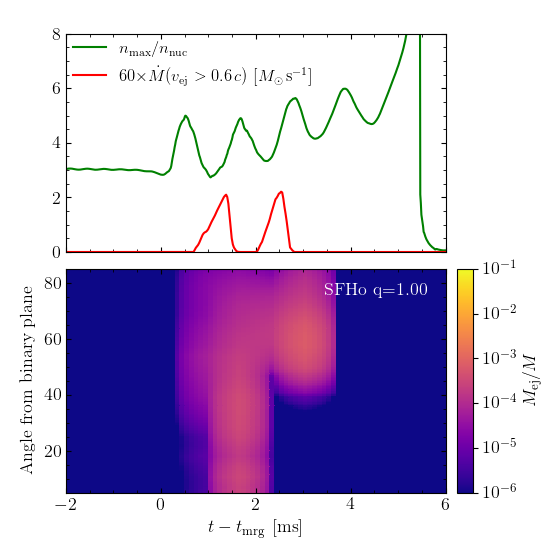
\includegraphics[height=7.3cm]{phd_figs/ejecta_dyn/fast_ejecta/SFHo_q100_LK_SR.pdf}
                    %\small{\textbf{Artist depiction of ejecta$^\text{\citep{Ascenzi:2020xqi}}$}}
            }};
        }
        \uncover<1->{ % <-> |
            \node (img1) [anchor=center,scale=1,opacity=1] at ([shift={(-3.2cm,-1.85cm)}]current page.center){
                \parbox{0.5\textwidth}{
                    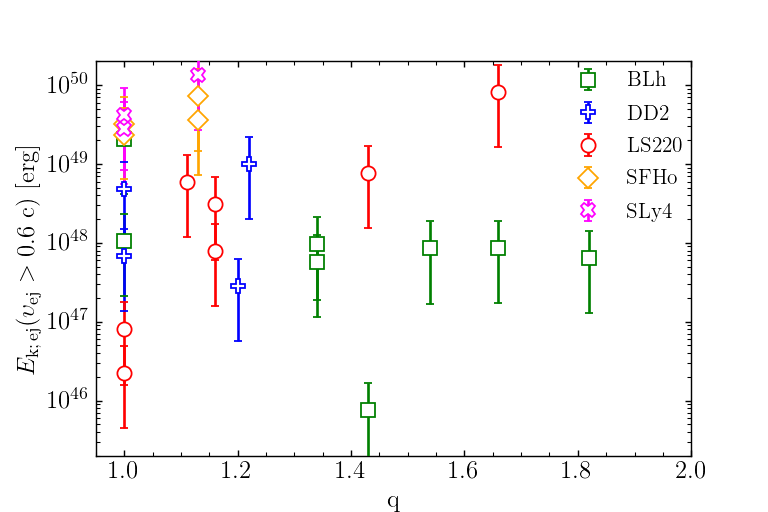
\includegraphics[height=4.4cm]{phd_figs/ejecta_dyn/fast_ejecta/scatter_ekej_vej06.pdf}
                    %\small{\textbf{Artist depiction of ejecta$^\text{\citep{Ascenzi:2020xqi}}$}}
            }};
        }
        
    \end{tikzpicture}
\end{frame}
%\section{Nucleosynthesis}
%%% --------------------------------------------------------------
%%
%% N U C L E O S Y N T H E S I S
%%
%% --------------------------------------------------------------
\begin{frame}{Nucleosynthesis} %% ---------- title 
\begin{tikzpicture}[overlay,remember picture]

    \uncover<1->{ % <-> |
        \node (t1) [anchor=center,scale=1,opacity=1] at ([shift={(-2.5cm,1.2cm)}]current page.center){
            \parbox{0.7\textwidth}{
                \textit{Heaviest elements in the Universe:}
                \begin{itemize}
                    \item Produced via \rproc{} \& \sproc{}%\footcite{Arcones:2010}.
                    \item Compact object mergers.
                    \item Magnetorotationally driven CCSN.
                \end{itemize}
                %                $M_{\text{wind}}$ is larger for more extended disks. % that in turn depend on thermal pressure
        }};
    }
    \uncover<1->{ % <-> |
    \node (t1) [anchor=center,scale=1,opacity=1] at ([shift={(-2.5cm,-2.2cm)}]current page.center){%([shift={(7.0cm,1.7cm)}]current page.center){
        \parbox{0.7\textwidth}{
            \textit{Observational constrains:}
            \begin{itemize}
                \item MP stars: \rproc{} material came early 
                \item UFG: support rare high-yeld events
                \item In the galaxy \rproc{} is uniform
                %\item broad distribution around the binary plane, high $0.1\lesssim \ayw\lesssim0.4$ peak ${\simeq}0.35$.%$\langle Y_e \rangle$
                %\item The low electron fraction material originates primarily at early times, when the material did not have enough time to be processed by neutrinos and before the outflow reaches quasi-steady state.
                %\item $\avw$ is ${\sim}0.1\,$c / ${\sim}0.2\,$c for soft/still \acp{EOS}
            \end{itemize}
    }};
    
    \uncover<1->{ % <-> |
        \node (img1) [anchor=center,scale=1,opacity=1] at ([shift={(4.15cm,-0.5cm)}]current page.center){
            \parbox{0.5\textwidth}{
                \includegraphics[height=5.5cm]{phd_figs/Fig_1_1_Lip.pdf}
                Observed abundances in Solar System\footcite{Lippuner:2018phd}%$^\text{\citep{Lippuner:2018phd}}$
%                    \caption{Observed abundances in our solar system as a function of mass number
%                    $A$. The lightest elements were created in the Big Bang and fusion in stars predominantly
%                    creates alpha elements. The iron peak is made in core-collapse and type
%                    Ia \acp{SN}. Elements beyond the iron peak are synthesized by the slow ($s$) and
%                    rapid ($r$) neutron capture processes. These processes produce three distinct double
%                    peaks. Abundance data from \citet{Lodders:2003}. (Adapted from \citet{Lippuner:2018phd})
%                }
        }};
    }
}
\end{tikzpicture}
\end{frame}

%Heaviest elements in the Universe
%\begin{itemize}
%    \item Produced via \rproc{} \& \sproc{}
%    \item For \rproc{} peaks at $A=80,\:130,\:194$ correspond to magic numbers (closed neutron shells)
%    \item Solar \rproc{} abundance pattern is consistent,
%\end{itemize}
%
%Possible $r$-process sites
%\begin{itemize}
%    \item Magnetorotationally driven \acp{CCSN} with collimated bipolar jet %\citep{Wheeler:2000,Akiyama:2003,Burrows:2007yx,Mosta:2014jaa,Mosta:2015}
%    \item Compact object mergers
%    \item \ac{BNS} and \ac{NSBH} mergers eject neutron rich material
%\end{itemize}
%
%Galactic chemical evolution
%\begin{itemize}
%    \item Very early source of \rproc{} material for the observed \rproc{} enrichment of \ac{MP} stars 
%    \item Observed rather uniform distribution of \rproc{} material in the Galaxy
%    \item \acp{UFG} observations point toward rare and high-yield events
%\end{itemize}
%
%Modeling the coupled nuclear reactions via \ac{NRN}
%\begin{itemize}
%    \item and \texttt{SkyNet} by \citet{Lippuner:2015gwa}\footnote{\url{https://bitbucket.org/jlippuner/skynet}}.
%    \item Observed rather uniform distribution of \rproc{} material in the Galaxy
%    \item \acp{UFG} observations point toward rare and high-yield events
%\end{itemize}
%
%\end{frame}

%% --------------------------------------------------------------
%%
%% N R N
%%
%% --------------------------------------------------------------

\begin{frame}{Nuclear reaction network \& parameterized model}

    %
    Key to model \nuc{}: nuclide interactions \& single particle reaction. %\citep[\eg][]{Hix:1999},
%    The key component of a \ac{NRN} is the interaction between two and more nuclides, 
%    that are characterized by \ac{RR} as well as single particle reactions, such as $\beta$-decay.
    %
%    Describing particle interaction and nuclide transmutation it is common to introduce the entrance 
%    and exit channels representing reactants and products. Then, \ac{RR} is defined as a speed 
%    at which a reaction proceeds per particle in the entrance channel. 
    %
    \textit{Abundance}, $Y_i$, evolution is\footcite{Hix:1999}%$^{\text{\citep{Hix:1999}}}$
    %
    \begin{equation*}
    Y_i = \frac{n_i}{n_B} = \frac{N_i}{N_B}, \hspace{5mm}
    \frac{\text{d}Y_i}{\text{d}t} = \sum\lambda_{\alpha}(-R_{i}^{\alpha}+P_{i}^{\alpha})N_{i}^{\alpha}\prod_{m\in\mathcal{R}_{\alpha}}Y_m^{N_{m}^{\alpha}}
    \end{equation*}
    %
%    $N_i$ and $N_B$ are the total numbers of particles 
%    where $\lambda_{\alpha}$ is the \ac{RR} of the forward process, $R_{i}^{\alpha}$ are reactants, 
%    $P_{i}^{\alpha}$ are products, $N_{i}^{\alpha}$ number of particles of the species $i$ involved 
%    and $Y_m^{N_{m}^{\alpha}}$ are the abundances of the particles of species $i$ involved 
    %
%    \texttt{SkyNet} solves a coupled, first-order, non-linear system of equation, 
%    Eq.~\eqref{eq:theory:nuc:abundance} for a given set of reaction rates $\lambda_{\alpha}$. 
%    The Eq.~\eqref{eq:theory:nuc:abundance} can be understood as following. 
%    The time derivative of the species $i$ abundances is given by the sum over all reactions, 
%    in which the species in question participate. Each reaction contribution consists of multiplies: 
%    \ac{RR}, a factor describing creation or destruction of particles (of species $i$), 
%    \ie, number of particles, and abundances of reactants. 
    %
    \texttt{SkyNet}\footcite{Lippuner:2015gwa}%$^{\text{\citep{Lippuner:2015gwa}}}$ solves 
    system of stiff \acp{ODE} %requiring implicit or specialized explicit solvers
    evolving the composition vector, $Y(t)$, %is evolved via implicit backward Euler method
    %The multi-dimensional, $N\times N$, root-finding problem is solved via Newton-Raphson method
    
    \textbf{Parameterized model}\footcite{Lippuner:2015gwa,Radice:2018pdn}%$^{\text{\citep{Lippuner:2015gwa,Radice:2018pdn}}}$ -- pre-computed \nuc{} for homologously expanding ejecta, $Y_i=f(Y_e, \tau, s)$, where
    %
    \begin{equation*}
        \rho(s, Y_e, T=6\text{GK})\Big(\frac{3\tau}{2.72 t}\Big)^3 = \rho(t) = \rho_E\Big(\frac{\upsilon_E}{r_E}t\Big)^{-3},
    \end{equation*}
    
%    \begin{equation}
%    \begin{aligned}
%    \text{Nucleo }\rho(t) &= \rho(s, Y_e, T=6\text{GK})\Big(\frac{3\tau}{2.72 t}\Big)^3 \\
%    \text{Ejecta }\rho(t) &= \rho_E\Big(\frac{\upsilon_E}{r_E}t\Big)^{-3},
%    \label{eq:nuc:rho_homolog}
%    \end{aligned}
%    \end{equation}
\end{frame}

%% --------------------------------------------------------------
%%
%% Results
%%
%% --------------------------------------------------------------

\begin{frame}{Spiral-wave wind contribute to the light \rproc{}\footcite{Nedora:2019jhl,Nedora:2020pak}}%$^\text{\citep{Nedora:2019jhl,Nedora:2020pak}}$} %% ---------- title 
    \begin{tikzpicture}[overlay,remember picture]
%    \uncover<1->{ % <-> |
%        \node (t1) [anchor=center,scale=1,opacity=1] at ([shift={(-0.8cm,2.6cm)}]current page.center){
%            \parbox{1.0\textwidth}{
%                Spiral-wave wind contribute to the light \rproc{}
%%                \begin{itemize}
%%                    \item Final $Y_i$ in \textit{total} ejecta are agreement with solar across all \rproc{} peaks. 
%%                    \item Actinide production depends strongly on the $Y_{e;\text{ej}}$, and thus, on the \mr{}.
%%                    %% The strongest neutrino heating occurs in the vicinity of the remnant at densities $\rho\sim10^{11}$~\gcm,
%%                \end{itemize}
%        }};
%    }
    \uncover<1->{ % <-> |
        \node (img1) [anchor=center,scale=1,opacity=1] at ([shift={(4.5cm,-0.8cm)}]current page.center){
            \parbox{0.6\textwidth}{
                \includegraphics[height=7.0cm]{phd_figs/nucleo/nucleo_dd2_blh.pdf}
        }};
    }
    \uncover<1->{ % <-> |
        \node (img1) [anchor=center,scale=1,opacity=1] at ([shift={(-4.0cm,-0.4cm)}]current page.center){
            \parbox{0.5\textwidth}{
                \includegraphics[height=6.5cm]{phd_figs/nucleo/cc_nucleo_BLh_total.pdf}
        }};
    }
    \end{tikzpicture}
\end{frame}
%\section{Kilonova}
%%% --------------------------------------------------------------
%%
%% K I L O N O V A
%%
%% --------------------------------------------------------------
\begin{frame}{Kilonova (kN)}
\begin{tikzpicture}[overlay,remember picture]
\uncover<1->{ % <-> |
    \node (t1) [anchor=center,scale=1,opacity=1] at ([shift={(-3.8cm,1.3cm)}]current page.center){
        \parbox{0.56\textwidth}{
            Thermal \ac{EM} counterpart to mergers, 
            powered by the decay of produced elements$^{\textcolor{gray}{\text{\cite{Metzger:2016pju}}}}$. \\
            Nuclear heating in ejecta, $\varepsilon_{\rm nuc}\propto t^{-\alpha}$. \\
            Ejecta expands and become transparent. \\
            % tdiff = \rho \kappa R^2 / c
            % Assuming constant opacty ; constant expansion speed v; uniform density \rho = m / (4pi R^3 / 3)
            $t_{\rm lc} = \sqrt{3\kappa m_{\rm ej} / (4 \pi c \upsilon_{\rm ej})}$, 
            $L_{\rm lc} = m_{\rm ej} \varepsilon_{\rm nuc}(t_{\rm lc})$; 
            % Characteristic luminocity us approx radioactive heating rate at this escape timescale
            % Larger, massive ejecta -- brighter lightcurve 
            % Opacity - bound bound transitions in d-shells in iron-group elements (low kappa) and f-shell in lanthinides (high kappa)
%            \begin{itemize}
%                \item Fast rise and decay
%                \item Strong dependency on composition
%                \item Dependency on the obs. angle
%            \end{itemize}
    }};
}

\uncover<1->{ % <-> |
    \node (t1) [anchor=center,scale=1,opacity=1] at ([shift={(-3.6cm,-1.5cm)}]current page.center){
        \parbox{0.60\textwidth}{
            \textbf{\AT{}}, counterpart to \GW{}$^{\textcolor{gray}{\text{\cite{Villar:2017wcc}}}}$ \\
            Two spatially distinct components$^{\textcolor{gray}{\text{\cite{Kasen:2017sxr}}}}$:
            \begin{itemize}
            \item low $\kappa$ (high $Y_e$) -- early \textcolor{blue}{"blue"} peak,
            \item high $\kappa$ (low $Y_e$) -- late \textcolor{red}{"red"} peak.
            \end{itemize}
    }};
}

\uncover<1->{ % <-> |
    \node (t1) [anchor=center,scale=1,opacity=1] at ([shift={(-3.6cm,-3.5cm)}]current page.center){
        \parbox{0.60\textwidth}{
            \textbf{Issue:} insufficient ejecta to explain early \textcolor{blue}{"blue"} early emission.
%            \begin{itemize}
%                \item Insufficient ejecta to explain early blue part.
%            \end{itemize}
    }};
}

\uncover<1-1>{ % <-> |
    \node (img1) [anchor=center,scale=1,opacity=1] at ([shift={(3.8cm,-0.2cm)}]current page.center){
        \parbox{0.5\textwidth}{
            \includegraphics[height=5.8cm]{figures/KasenBolKn.pdf}
            %\includegraphics[height=5.5cm]{phd_figs/viller_mkn_model.png}
            
    }};
}
\uncover<2->{ % <-> |
    \node (img1) [anchor=center,scale=1,opacity=1] at ([shift={(4.5cm,-0.5cm)}]current page.center){
        \parbox{0.45\textwidth}{
            \includegraphics[height=4.8cm]{phd_figs/mkn__albino2.pdf} \\
            \textbf{Model}: multicomponent, anisotropic semi-analytical. \texttt{MKN} code$^{\textcolor{gray}{\text{\cite{Perego:2017wtu}}}}$\\ 
            Black-body radiation; freely expanding ejecta
            % Ejecta compoenents in \texttt{MKN}
            %            \caption{Graphic representation of the analyzed
                %                ejecta profiles for isotropic and anisotropic cases
                %                from an azimuthal perspective and for a fixed moment of time.
                %                The black dot represents the remnant and the dashed line is the projected orbital
                %                plane of the binary. The shadowed areas describe the ejecta profiles: the shape
                %                characterizes the mass distribution, while the colors refer to 
                %                the prior assumptions on the opacity parameter.
                %                In particular, blue regions denote opacities lower than $5~\igscm$,
                %                red regions refer to opacities greater than $5~\igscm$,
                %                and oranges areas indicate a broadly distributed opacity.
                %                All shells are isotropically expanding with a constant velocity.
                %                (Adapted from \citet{Breschi:2021wzr})
        }};
    }

%        \parbox{0.7\textwidth}{
%    Key components %$M_{\rm ej}$, $\upsilon_{\rm ej}$, $Y_{e\rm; ej}$
%    \begin{itemize}
%        %            
%        \item Energy generation \& energy release:
%        %            Key ejecta properties $M$, $\upsilon$, $Y_e$, that determine \\
%        %            heating, $\dot{Q}(t)$, thermalization, opacity
%        %            
%        %            \begin{equation*}
%            %            \dot{Q}_i \propto \exp(-t/\tau_i), \,\, 
%            %            \dot{Q}_{LP} = f \frac{M c^2}{t}, \,\,  
%            \item nuclear heating $\dot{Q}_{r,\upsilon} = dM_{\upsilon}X_{r,\upsilon}\dot{e}_{r}(t)$,
%            
%            %            \end{equation*}
%        %            where $f$ is free parameter and $M$ is the ejecta mass.
%        %            the $dM_{\upsilon}$ is ejecta mass layer (with velocity $\upsilon$).
%        %            The layer has a fraction $X{r,\upsilon}$ of \rproc{} elements, 
%        where specific heating, $\dot{e}_r(t)$, requires detailed \nuc{}.
%        %            for which is from detailed \nuc{} calculations \citep{Korobkin:2012uy}
%        
%        %            For the radiation the diffusion timescale is
%        %            \begin{equation}
%            %            \tau = \rho \kappa R = \frac{3}{4}\frac{M\kappa}{4\pi R^2} \hspace{5mm} 
%            %            t_{diff} \approx \frac{R}{c}\tau = \frac{3}{4}\frac{M\kappa}{4\pi c R} = \frac{3}{4}\frac{M\kappa}{\pi c \upsilon t}
%            %            \end{equation}
%        %            where $M$ is the ejecta mass, $\kappa$ is the opacity (cross section per unit mass), 
%        %            $\rho$ is the density, \eg, $\rho=3M/(4\pi R^3)$ is the mean density.
%        
%        \item Emission peaks when $t=t_{\rm diff}=f(\kappa)$ Arnett's law$^\text{\textcolor{gray}{\citep{Arnett:1982}}}$.
%        %            \begin{equation}
%            %            t_{peak} = \Big(\frac{3}{4}\frac{1}{\beta}\frac{M\kappa}{\pi \upsilon c}\Big)^{1/2}
%            %            \end{equation}
%        %            and the peak luminocity is set by $\dot{Q}(t)$
%        
%        Opacity $\kappa$ requries detailed atomic calculations
%        \\
%        %
%        %            \begin{equation*}
%            %            F_{\nu}(\mathbf{n},t) = \int_{\mathbf{n}_{\Omega} \cdot \mathbf{n}> 0} 
%            %            \left( \frac{R_{\text{ph}}(\Omega,t)}{D_L} \right)^2  B_{\nu}(T_{\text{eff}}(\Omega,t))~\mathbf{n} \cdot  \dd\boldsymbol{\Omega} 
%            %            \end{equation*}
%        
%        %            where $\mathbf{n}$ is the unitary vector along the line of sight, $\mathbf{n}_{\Omega}$ is the unitary 
%        %            vector spanning the solid angle $\Omega$, $D_L$ is the luminosity distance, $R_{\text{ph}}$ is the local 
%        %            radial coordinate of the photospheric surface, and $B_{\nu}(T_{\rm eff})$ is the spectral radiance at 
%        %            frequency $\nu$ for a surface of temperature $T_{\text{eff}}$
%        
%        %%%% Magnitude
%        %            We also make use of the apparent AB magnitude mag$_b$ in a given photometric band $b$, defined as:
%        
%        %            \begin{equation*}
%            %            \text{mag}_b(\mathbf{n},t) = -2.5 \log_{10}\left( F_{\nu_b}(\mathbf{n},t) \right)-48.6\,,
%            %            \end{equation*}
%        %            where $\nu_b$ is the effective central frequency of band $b$.
%    \end{itemize}
%    
%    
%    %             \texttt{MKN} code$^\text{\citep{Perego:2017wtu}}$ \\
%    %             multicomponent, anisotropic semi-analytical model \\
%    %             geometry imported from \ac{NR} simulations \\
%    %             opacities \& heating rates from from dedicated studies 
%    %             \citep{Tanaka:2019iqp,Korobkin:2012uy} \\
%    
%    


\end{tikzpicture}
\end{frame}

%\begin{frame}{Introduction} %% ---------- title 
%Thermal counterpart, powered by the decay of newly synthesized heavy elements %\citep[\eg][]{Li:1998bw,Kulkarni:2005jw,Metzger:2010,Roberts:2011,Metzger:2016pju,Wollaeger:2017ahm}
%The only unambiguous detection \AT{}
%%\citep{Arcavi:2017xiz,Coulter:2017wya,Drout:2017ijr,Evans:2017mmy,Hallinan:2017woc,Kasliwal:2017ngb,
%%    Nicholl:2017ahq,Smartt:2017fuw,Soares-santos:2017lru,Tanvir:2017pws,
%%    Troja:2017nqp,Mooley:2018dlz,Ruan:2017bha,Lyman:2018qjg}. 
%very well sampled.
%Distinguished blue/red components attributed to low/high opacity material, %\citep[\eg][]{Villar:2017wcc}
%%lanthanides $(58\leq Z \leq71)$ and actinides $(90\leq Z \leq 103)$, that have an open $f$-shell 
%or high/low $Y_e$ material
%%
%%Other candidates 
%%GRB130603B, \citep{Berger:2013wna,Tanvir:2013pia}, 
%%GRB060614 \citep{Jin:2015txa,Yang:2015pha}, 
%%GRB050709 \citep{Jin:2016pnm}. 
%
%%The peak luminosity \textit{Arnett's Law} \citep{Arnett:1982}.
%%In this simplified picture, three ingredients are required to understand the observations of \ac{kN}. 
%%These are 
%%\begin{itemize}
%%    \item The ejecta properties: $M$, $\upsilon$, $Y_e$,
%%    \item The composition of the expanding ejecta and its optical opacity 
%%        \begin{itemize}
%%            \item \ac{FIR} -- the free-free absorption 
%%            \item \ac{IR}/optical -- bound-bound ()line opacities, approximated with effective opacity)
%%            \item \ac{UV}/X-ray -- bound-free transitions dominate the opacity (when ejecta is neutral)
%%        \end{itemize}
%%    
%%    (bound-bound opacities dominate) % line opacities to the effective opacity.
%%    
%%    \item Dominant sources of energy within the ejecta, heating rate $\dot{Q}(t)$, and how 
%%    efficient this energy thermalizes.
%%\end{itemize}
%
%\end{frame}

%% ---

%\begin{frame}{Method}
%    For a single spherical shell, the emission is cahacterized 
%    \begin{equation}
%        \dot{Q}_i \propto \exp(-t/\tau_i), \,\, \dot{Q}_{LP} = f \frac{M c^2}{t}, \,\,  \dot{Q}_{r,\upsilon} = dM_{\upsilon}X_{r,\upsilon}\dot{e}_{r}(t).
%    \end{equation}
%    where $f$ is free parameter and $M$ is the ejecta mass.
%    the $dM_{\upsilon}$ is ejecta mass layer (with velocity $\upsilon$).
%    The layer has a fraction $X{r,\upsilon}$ of \rproc{} elements, specific heating, $\dot{e}_r(t)$,  
%    for which is from detailed \nuc{} calculations \citep{Korobkin:2012uy}
%    
%    For the radiation the diffusion timescale is
%    \begin{equation}
%    \tau = \rho \kappa R = \frac{3}{4}\frac{M\kappa}{4\pi R^2} \hspace{5mm} 
%    t_{diff} \approx \frac{R}{c}\tau = \frac{3}{4}\frac{M\kappa}{4\pi c R} = \frac{3}{4}\frac{M\kappa}{\pi c \upsilon t}
%    \end{equation}
%    where $M$ is the ejecta mass, $\kappa$ is the opacity (cross section per unit mass), 
%    $\rho$ is the density, \eg, $\rho=3M/(4\pi R^3)$ is the mean density.
%    
%    Emission peaks when $t=t_{diff}$ \citep{Arnett:1982}.
%    \begin{equation}
%    t_{peak} = \Big(\frac{3}{4}\frac{1}{\beta}\frac{M\kappa}{\pi \upsilon c}\Big)^{1/2}
%    \end{equation}
%    and the peak luminocity is set by $\dot{Q}(t)$
%    
%    In this simplified picture, three ingredients are required to understand the observations of \ac{kN}. 
%    These are 
%    \begin{itemize}
%        \item The ejecta properties: $M$, $\upsilon$, $Y_e$,
%        \item The composition of the expanding ejecta and its optical opacity.
%        \item Dominant sources of energy within the ejecta, heating rate $\dot{Q}(t)$, and how 
%        efficient this energy thermalizes.
%    \end{itemize}
%    
%    \begin{equation}
%    \label{eq:spectral_flux}
%    F_{\nu}(\mathbf{n},t) = \int_{\mathbf{n}_{\Omega} \cdot \mathbf{n}> 0} 
%    \left( \frac{R_{\text{ph}}(\Omega,t)}{D_L} \right)^2  B_{\nu}(T_{\text{eff}}(\Omega,t))~\mathbf{n} \cdot  \dd\boldsymbol{\Omega} 
%    \end{equation}
%    %
%    where $\mathbf{n}$ is the unitary vector along the line of sight, $\mathbf{n}_{\Omega}$ is the unitary 
%    vector spanning the solid angle $\Omega$, $D_L$ is the luminosity distance, $R_{\text{ph}}$ is the local 
%    radial coordinate of the photospheric surface, and $B_{\nu}(T_{\rm eff})$ is the spectral radiance at 
%    frequency $\nu$ for a surface of temperature $T_{\text{eff}}$
%    
%    \begin{figure}
%        \centering 
%        \includegraphics[width=0.48\textwidth]{profiles_op.pdf}
%        \caption{Graphic representation of the analyzed
%            ejecta profiles for isotropic and anisotropic cases
%            from an azimuthal perspective and for a fixed moment of time.
%            The black dot represents the remnant and the dashed line is the projected orbital
%            plane of the binary. The shadowed areas describe the ejecta profiles: the shape
%            characterizes the mass distribution, while the colors refer to 
%            the prior assumptions on the opacity parameter.
%            In particular, blue regions denote opacities lower than $5~\igscm$,
%            red regions refer to opacities greater than $5~\igscm$,
%            and oranges areas indicate a broadly distributed opacity.
%            All shells are isotropically expanding with a constant velocity.
%            (Adapted from \citet{Breschi:2021wzr})
%        }
%        \label{fig:cartoon}
%    \end{figure}
%    
%\end{frame}

%% --------------------------------------------------------------
%%
%% Method
%%
%% --------------------------------------------------------------

%\begin{frame}{Kilonova code} %% ---------- title 
%
%\begin{tikzpicture}[overlay,remember picture]
%
%\uncover<1->{ % <-> |
%    \node (t1) [anchor=center,scale=1,opacity=1] at ([shift={(-3.4cm,-0.6cm)}]current page.center){
%        \parbox{0.63\textwidth}{
%            \texttt{MKN code}: 
%            multicomponent, anisotropic semi-analytical model $^{\textcolor{gray}{\text{\cite{Perego:2017wtu}}}}$
%            \begin{itemize}
%                \item Ejecta $m(\theta)$, $\upsilon(\theta)$, $\kappa(\theta)$
%                \item Nuclear heating rate $\varepsilon_{\rm nuc} = f(t)$, 
%                \item Mean plank opacities from atomic calculation$^{\textcolor{gray}{\text{\cite{Tanaka:2019iqp}}}}$
%                \item Black-body radiation with $T_{\rm eff}$ from $R_{\rm ph}$
%%                \item geometry imported from \ac{NR} simulations 
%%                \item opacities \& heating rates from from dedicated studies$^\text{\textcolor{gray}{\citep{Tanaka:2019iqp,Korobkin:2012uy}}}$ 
%            \end{itemize}
%    }};
%}
%
%\uncover<1->{ % <-> |
%    \node (img1) [anchor=center,scale=1,opacity=1] at ([shift={(5.1cm,-0.2cm)}]current page.center){
%        \parbox{0.5\textwidth}{
%            \includegraphics[height=5cm]{phd_figs/mkn__albino2.pdf}
%            
%            \hspace*{10mm} Ejecta compoenents in \texttt{MKN}
%%            \caption{Graphic representation of the analyzed
%%                ejecta profiles for isotropic and anisotropic cases
%%                from an azimuthal perspective and for a fixed moment of time.
%%                The black dot represents the remnant and the dashed line is the projected orbital
%%                plane of the binary. The shadowed areas describe the ejecta profiles: the shape
%%                characterizes the mass distribution, while the colors refer to 
%%                the prior assumptions on the opacity parameter.
%%                In particular, blue regions denote opacities lower than $5~\igscm$,
%%                red regions refer to opacities greater than $5~\igscm$,
%%                and oranges areas indicate a broadly distributed opacity.
%%                All shells are isotropically expanding with a constant velocity.
%%                (Adapted from \citet{Breschi:2021wzr})
%    }};
%}
%
%%\texttt{MKN} code
%%\uncover<1->{ % <-> |
%%    \node (t2) [anchor=center,scale=1,opacity=1] at ([shift={(-3.8cm,-1.8cm)}]current page.center){
%%        \parbox{0.6\textwidth}{
%%            \begin{itemize}
%%            \item multicomponent, anisotropic semi-analytical 
%%            \end{itemize}
%%    }};
%%}
%
%\end{tikzpicture}
%
%\end{frame}



%% --------------------------------------------------------------
%%
%% Results
%%
%% --------------------------------------------------------------

%\begin{frame}{EM signature of the \swind{}} %% ---------- title 
%
%\begin{tikzpicture}[overlay,remember picture]
%
%\uncover<1->{ % <-> |
%    \node (t1) [anchor=center,scale=1,opacity=1] at ([shift={(-4.1cm,1.0cm)}]current page.center){
%        \parbox{0.55\textwidth}{
%            Dynamical ejecta cannot explain early blue emission \\
%            
%            Contribution from the \swind{} is natural
%            
%    }};
%}
%
%
%
%\uncover<1->{ % <-> |
%    \node (img1) [anchor=center,scale=1,opacity=1] at ([shift={(3.4cm,-0.2cm)}]current page.center){
%        \parbox{0.5\textwidth}{
%            \includegraphics[height=5.5cm]{kilonova/mkn_dd2_band.pdf}
%%            Bolometric kN light curves in three representative bands from blue to
%%            infrared for the two simulations with turbulence viscosity compared to
%%            \AT{} data from~\citep{Villar:2017wcc}.
%%            The color gradient is the effect related to different
%%            \ac{SWW} masses, that suggests possible variations of the light
%%            curves for different \ac{BNS}. The band is computed by extracting the
%%            \ac{SWW} mass from DD2 every $10$~ms until the end of the simulation, and
%%            then by linearly extrapolating the data to $250$~ms.
%%            (Adapted from \citet{Nedora:2019jhl})
%    }};
%}
%
%Low opacity, fast \ac{SWW} 
%\uncover<1->{ % <-> |
%    \node (t2) [anchor=center,scale=1,opacity=1] at ([shift={(-3.8cm,-1.8cm)}]current page.center){
%        \parbox{0.6\textwidth}{
%            \begin{itemize}
%            \item Dynamical ejecta cannot explain early blue emission
%            \item Probe of remnant dynamics, lifetime and EOS
%            \end{itemize}
%    }};
%}
%
%\end{tikzpicture}
%
%\end{frame}





\begin{frame}{Spiral-wave wind for the blue kilonova$^{\text{\textcolor{gray}{\cite{Nedora:2019jhl,Nedora:2020pak}}}}$} %% ---------- title 

\begin{tikzpicture}[overlay,remember picture]

\uncover<1->{ % <-> |
    \node (t1) [anchor=center,scale=1,opacity=1] at ([shift={(-0.8cm,1.8cm)}]current page.center){
        \parbox{1.0\textwidth}{
            \begin{itemize}
            \item Dynamical ejecta cannot explain early blue emission
            \item Probe of remnant dynamics, lifetime and EOS
            \end{itemize}
    }};
}

\uncover<1->{ % <-> |
    \node (img1) [anchor=center,scale=1,opacity=1] at ([shift={(-2.0cm,-1.65cm)}]current page.center){
        \parbox{0.5\textwidth}{
            \includegraphics[height=5cm]{phd_figs/ejecta_dyn/summary/ej_mej_yeej_our2.pdf}
    }};
}

\uncover<1->{ % <-> |
    \node (img1) [anchor=center,scale=1,opacity=1] at ([shift={(3.8cm,-1.5cm)}]current page.center){
        \parbox{0.5\textwidth}{
            \includegraphics[height=5.15cm]{phd_figs/kilonova/mkn_dd2_band.pdf}
    }};
}


\end{tikzpicture}

\end{frame}

%\begin{figure*}[t]
%    \centering 
%    \includegraphics[width=0.48\textwidth]{ejecta_dyn/summary/ej_mej_vej_our2.pdf}
%    \includegraphics[width=0.48\textwidth]{ejecta_dyn/summary/ej_mej_yeej_our2.pdf}
%    \caption{
%        Summary of the ejecta properties of our models.
%        %
%        Diamonds mark the dynamical ejecta, crosses include the
%        contribution of the \swind{} for the long-lived models, 
%        triangles are an estimate of the total ejecta mass on a secular
%        timescale, assuming $40\%$ of the disk mass is unbounded on
%        secular timescales.         
%        The ejecta mass is shown is terms of the mass-averaged velocity
%        (left) and of the averaged electron fraction (right).
%        %
%        The filled blue and red patches are the expected values of
%        ejecta mass and velocity for blue and red components of
%        AT2017gfo compiled by \cite{Siegel:2019mlp}, based on
%        \cite{Villar:2017wcc}. 
%        Adopted from \citet{Nedora:2020pak}.
%    }
%    %
%    \label{fig:ejecta:dyn:ds_sww}
%\end{figure*}

%\section{Afterglows}
%%% --------------------------------------------------------------
%%
%% A F T E R G L O W
%%
%% --------------------------------------------------------------
\begin{frame}{Introduction}
\begin{tikzpicture}[overlay,remember picture]
\uncover<1->{ % <-> |
    \node (t1) [anchor=center,scale=1,opacity=1] at ([shift={(-2.9cm,1.3cm)}]current page.center){
        \parbox{0.70\textwidth}{
            GRBs, cocoon, ejecta produce afterglow \\
            Synchrotron emission arising when a shock propagates through ISM
            \begin{itemize}
            \item Trace physics of jet formation
            \item Information on the fastest ejecta
            \end{itemize}
    }};
}

\uncover<1->{ % <-> |
    \node (t1) [anchor=center,scale=1,opacity=1] at ([shift={(-2.9cm,-2.0cm)}]current page.center){
        \parbox{0.70\textwidth}{
            \GRB{}, non-thermal EM counterpart to \GW{}
            \begin{itemize}
            \item Very long follow-up
            \item Structured jet model explans slow rise
            \item Spectrums is described by power law$^{(*)}$
            \end{itemize}
    }};
}

%\uncover<1->{ % <-> |
%    \node (t1) [anchor=center,scale=1,opacity=1] at ([shift={(-3.6cm,-3.5cm)}]current page.center){
%        \parbox{0.60\textwidth}{
%            Several open questions
%            \begin{itemize}
%            \item Insufficient ejecta to explain early blue part.
%            \end{itemize}
%    }};
%}

\uncover<1->{ % <-> |
    \node (img1) [anchor=center,scale=1,opacity=1] at ([shift={(6.0cm,-0.8cm)}]current page.center){
        \parbox{0.5\textwidth}{
            \includegraphics[height=6.3cm]{jet_ascenci20.pdf}

            Artist depiction of ejecta$^\text{\citep{Ascenzi:2020xqi}}$
    }};
}
\end{tikzpicture}
\end{frame}

%% =======================================================
%%
%%                   Method
%%
%% =======================================================

\begin{frame}{Method} %% ---------- title 

\begin{tikzpicture}[overlay,remember picture]

\uncover<1->{ % <-> |
    \node (t1) [anchor=center,scale=1,opacity=1] at ([shift={(-3.9cm,-0.7cm)}]current page.center){
        \parbox{0.53\textwidth}{
            Passing through the cold ISM, shock front 
            \begin{itemize}
                \item randomizes the particles' $\vec{\upsilon}$,
                \item compresses the plasma,
                \item amplifies the magnetic fields 
                \item accelerates the inbound particles % to a power-law distribution function.
            \end{itemize}
            
            \textbf{Dynamics} --
            %A relativistic shock propagating into a cold upstream medium.
            $3$ conservation laws: baryon number, energy, momentum fluxes across shock front.
%            The latter two $T^{\mu\nu} = (\rho' c^2 + p') u^{\mu} u^{\nu} + p' g^{\mu\nu},$
            %
%            These equations can be written as 
            %
%            \begin{equation} % subequations
%            \begin{aligned} % align
%            \frac{e_2'}{n_2'} &= (\gamma_{21} - 1)m_p c^2 \\
%            \frac{n_2'}{n_1'} &= \frac{\hat{\gamma}\gamma_{21} + 1}{\hat{\gamma}-1} \\
%            \gamma_{1s}^2 &= \frac{(\gamma_{21} + 1) [\hat{\gamma}(\gamma_{21}-1)+1]^2}{\hat{\gamma}(2-\hat{\gamma})(\gamma_{21}-1)+2}
%            \end{aligned} % align
%            \label{eq:afterglow:blast}
%            \end{equation} % subequations
            %
%            \begin{figure*}[t]
%            \centering 
%            \includegraphics[width=0.45\textwidth]{Fig_8_KZ.pdf}
%            \caption{
%                This is a schematic sketch of a pair of shocks produced when a relativistic
%                jet from a \ac{GRB} collides with the \ac{CBM}, as viewed from the
%                rest frame of unshocked \ac{CBM}. Regions 2 \& 3 represent shocked \ac{CBM} and \ac{GRB}
%                jet respectively. They move together with the same \ac{LF} ($\gamma_2$, as viewed
%                by a stationary observer in the unshocked \ac{CBM}), and have the same pressure but
%                different densities.
%                (Adapted from \citet{Kumar:2014upa}, figure~8)
%            }
%            \label{fig:aafg:theory:sr8}
%            \end{figure*}
            %
%            where subscripts $2$ and $1$ stand for downstream and upstream respectively, 
%            $e'$ is the internal energy density, $n'$ is the proton number density, 
%            $\gamma_{21}$ is the relative \ac{LF} of plasma in region 
%            $2$ with respect to the region $1$
%            $\gamma_{1s}$ is the relative \ac{LF} of plasma in region $1$ with respect to the shock front,
%            $\hat{\gamma}$ is the adiabatic index of the fluid, for the ideal, relativistic 
%            fluid is $\hat{\gamma}=4/3$ and subrelativisitc $\hat{\gamma}=5/3$.
%            The $2$ and $1$ regions are also shown in Fig.~\ref{fig:aafg:theory:sr8} 
%            (see also \cite{Nava:2013} for a more comprehensive take).
%            %
%            Solving the system Eq.~\eqref{eq:afterglow:blast} gives the full evolution 
%            of the \blast{}. 
            
            \textbf{Electrons:} continuity eq. in energy space 
            \begin{equation*}
            \frac{\partial }{\partial t}\frac{d n_e}{d\gamma_e} + \frac{\partial}{\partial \gamma_e}\Big[ \dot{\gamma_e}\frac{dn_e}{d\gamma_e} \Big] = S(\gamma_e), \rightarrow \frac{d n_e}{d\gamma_e} \propto \gamma^{-p}
            \end{equation*}
            %
            Charactersitc, $\gamma_c$ , $\gamma_M$ , $\gamma_m$
            %
%            where $\dot{\gamma_e} = -\sigma_T B^2 \gamma_e^2 / (6\pi m_e c)$ is the rate at 
%            which electron \ac{LF} changes due to losses, $S(\gamma_e)$ is the injection 
%            rate of electrons into the system.
%            %
%            Assume that the minimum \ac{LF} of injected electrons is $\gamma_m$, \eg, 
%            where $S(\gamma_e) = 0$ for $\gamma_e < \gamma_m$.
%            %
%            \begin{equation}
%            dn_e/d\gamma_e \propto 
%            \begin{cases}
%            \gamma_e^{-2} &\text{ if } \gamma_c < \gamma_e < \gamma_m, \\
%            \gamma_e^{-p-1} &\text{ if } \gamma_e > \gamma_c > \gamma_m
%            \end{cases}
%            \label{eq:afterglow:elec_dist}
%            \end{equation}
            
    }};

    \node (t2) [anchor=center,scale=1,opacity=1] at ([shift={(3.9cm,-0.7cm)}]current page.center){
    \parbox{0.53\textwidth}{
        \textbf{Synchrotron emission} %\citep{RybickiLightman:1985} --
        %
        \begin{equation*}
        P_{syn} = \frac{2q^4 E^2}{3c^3 m_e^2}
        \,
        \omega_{syn}\sim\frac{qB\gamma_e^2}{m_e c}
        %\,
        %P_{syn}(\nu_{syn}) \sim P_{syn}/\nu_{syn}
        \end{equation*}
        %
        \begin{equation*}
        f_{\nu} = \int_{\gamma_{\nu}}^{\infty} d\gamma_e \frac{dn_e}{d\gamma_e}P_{syn}(\nu) 
        \end{equation*}
        
        \textbf{EATS}
        %
        \begin{equation*}
        F(\nu,t) = c\int_0^{\theta}\int_{0}^{r}\frac{P'(\nu',t_{em},r)}{\Gamma^2(1-\beta\cos\theta)^2}r^2 dr d\cos\theta
        \end{equation*}
        with $c = (1+z) / (2d_L^2)$
}};
}
\end{tikzpicture}
\end{frame}

%% =======================================================
%%
%%                   Method :: Code
%%
%% =======================================================

\begin{frame}{Method :: \texttt{PyBlastAfterglow}} %% ---------- title 

\begin{tikzpicture}[overlay,remember picture]

\uncover<1->{ % <-> |
    \node (t1) [anchor=center,scale=1,opacity=1] at ([shift={(-3.9cm,-0.7cm)}]current page.center){
        \parbox{0.53\textwidth}{
            \textbf{Blast wave dynamics} 
            \begin{itemize}
                \item[\textcolor{black}{$\blacksquare$}] uniform ISM; FS only$^\text{\citep{Peer:2012}}$
                \item[\textcolor{blue}{$\blacksquare$}] $\forall$ ISM, FS/RS; Rad.Loss$^\text{\citep{Nava:2013}}$
            \end{itemize}
            \textbf{Transrelativisitc Equation of state}
            \begin{itemize}
                \item[\textcolor{black}{$\blacksquare$}]Assymptic$^\text{\citep{Nava:2013}}$
                \item[\textcolor{blue}{$\blacksquare$}] HD-simulation informed$^\text{\citep{Peer:2012}}$
            \end{itemize}
            \textbf{Lateral Spreading}
            \begin{itemize}
                \item[\textcolor{black}{$\blacksquare$}] Speed of sound limited$^\text{\citep{Huang:1999di}}$
                \item[\textcolor{blue}{$\blacksquare$}] 2D HD -informed$^\text{\citep{Granot:2012}}$ 
            \end{itemize}
    }};
}

\uncover<1->{ % <-> |
    \node (t2) [anchor=center,scale=1,opacity=1] at ([shift={(3.9cm,-0.7cm)}]current page.center){
        \parbox{0.53\textwidth}{
            \textbf{Electron distribution} 
            \begin{itemize}
                \item[\textcolor{black}{$\blacksquare$}] Simple 2-segment \ac{BPL}
                \item[\textcolor{blue}{$\blacksquare$}] \ac{BPL} with accurate crit. Lorentz. Fact.
                \item[\textcolor{gray}{$\blacksquare$}] $\forall$ segmented electron distribution
            \end{itemize}
            \textbf{Synchrotron spectrum}
            \begin{itemize}
                \item[\textcolor{black}{$\blacksquare$}] 3-segment \ac{BPL} $^\text{\citep{Sari:1997qe}}$
                \item[\textcolor{blue}{$\blacksquare$}] Smooth \ac{BPL}$^\text{\citep{Johannesson:2006zs}}$ + SSA$^\text{\citep{Johannesson:2018cdl}}$
                \item[\textcolor{gray}{$\blacksquare$}] Direct integration of syntronton function$^\text{\citep{Dermer:2009}}$
            \end{itemize}
            \textbf{Equal time arrival surface integrator}
            \begin{itemize}
                \item[\textcolor{black}{$\blacksquare$}] Piece-wise sum (including $\mathcal{D}$)$^\text{\citep{Fernandez:2021xce}}$
            \end{itemize}
    }};
}
\end{tikzpicture}
\end{frame}

%% ---------------------------------------------------------------------------------------------

%\begin{frame}{EM signature of the dynamical ejecta} %% ---------- title 
%
%\begin{tikzpicture}[overlay,remember picture]
%
%\uncover<1->{ % <-> |
%    \node (t1) [anchor=center,scale=1,opacity=1] at ([shift={(-4.1cm,1.0cm)}]current page.center){
%        \parbox{0.55\textwidth}{
%            \begin{itemize}
%                \item Kilonova afterglow is consistent with rebrightneing of \GW{}
%                \item models with $q>1$ and moderately soft \ac{EOS} fit better
%            \end{itemize}
%    }};
%}
%
%
%
%\uncover<1->{ % <-> |
%    \node (img1) [anchor=center,scale=1,opacity=1] at ([shift={(3.8cm,0.2cm)}]current page.center){
%        \parbox{0.5\textwidth}{
%            \includegraphics[height=5.0cm]{kn_afterglow/best_xray_obs_representative_all_eos.pdf}
%            %            Bolometric kN light curves in three representative bands from blue to
%            %            infrared for the two simulations with turbulence viscosity compared to
%            %            \AT{} data from~\citep{Villar:2017wcc}.
%            %            The color gradient is the effect related to different
%            %            \ac{SWW} masses, that suggests possible variations of the light
%            %            curves for different \ac{BNS}. The band is computed by extracting the
%            %            \ac{SWW} mass from DD2 every $10$~ms until the end of the simulation, and
%            %            then by linearly extrapolating the data to $250$~ms.
%            %            (Adapted from \citet{Nedora:2019jhl})
%    }};
%}
%
%Low opacity, fast \ac{SWW} 
%\uncover<1->{ % <-> |
%    \node (t2) [anchor=center,scale=1,opacity=1] at ([shift={(-3.8cm,-1.8cm)}]current page.center){
%        \parbox{0.6\textwidth}{
%            \begin{itemize}
%            \item Kilonova afterglow is consistent with rebrightneing of \GW{}
%            \item Models with $q>1$ and moderately soft \ac{EOS} fit better
%            \end{itemize}
%    }};
%}
%
%\end{tikzpicture}
%
%\end{frame}


%% =======================================================
%%
%%                   Result
%%
%% =======================================================

\begin{frame}{Kilonova afterglow for \GRB{} rebrightening} %% ---------- title 

\begin{tikzpicture}[overlay,remember picture]

\uncover<1->{ % <-> |
    \node (t1) [anchor=center,scale=1,opacity=1] at ([shift={(-0.8cm,1.8cm)}]current page.center){
        \parbox{1.0\textwidth}{
            \begin{itemize}
            \item Kilonova afterglow is consistent with rebrightneing of \GW{}
            \item Models with $q>1$ and moderately soft \ac{EOS} fit better
            \end{itemize}
    }};
}

\uncover<1->{ % <-> |
    \node (img1) [anchor=center,scale=1,opacity=1] at ([shift={(-4.0cm,-1.5cm)}]current page.center){
        \parbox{0.5\textwidth}{
            \includegraphics[height=5cm]{kn_afterglow/best_xray_obs_representative_all_eos.pdf}
    }};
}

\uncover<1->{ % <-> |
    \node (img1) [anchor=center,scale=1,opacity=1] at ([shift={(4.0cm,-1.5cm)}]current page.center){
        \parbox{0.5\textwidth}{
            \includegraphics[height=5cm]{kn_afterglow/scatter_lightcurve_tpeak_vs_lambda.pdf}
    }};
}

\end{tikzpicture}

\end{frame}
%\section{Statistics}
%%% --------------------------------------------------------------
%%
%% K I L O N O V A
%%
%% --------------------------------------------------------------

%% Our models
\newcommand{\DSrefset}{\texttt{M0RefSet}} 
%% large leackage dataset that we usually compare to
\newcommand{\DSheatcool}{\texttt{M0/M1Set}} 
%% all datasets with neutrino absorption
\newcommand{\DScool}{\texttt{LeakSet}}
%% all datasets with leaakge
\newcommand{\DSnone}{\texttt{NoNusSet}}

\def\chid{\chi_{\nu}^2}
\def\non{\nonumber}

%\begin{frame}{Motivation \& Method}
%    \begin{tikzpicture}[overlay,remember picture]
%    \uncover<1->{ % <-> |
%        \node (t1) [anchor=center,scale=1,opacity=1] at ([shift={(-3.6cm,0.5cm)}]current page.center){
%            \parbox{0.60\textwidth}{
%                Link between intrinsic binary parameters \&
%                properties of the EM signal.
%                
%                Fitting formulae to the ejecta and \pmerg{} remnants properties
%        }};
%    }
%
%    \uncover<1->{ % <-> |
%        \node (t1) [anchor=center,scale=1,opacity=1] at ([shift={(-3.6cm,0.5cm)}]current page.center){
%            \parbox{0.60\textwidth}{
%                Compile available NR BNS models into 
%                \DSheatcool{}, \DSrefset{}, \DScool{}, \DSnone{}
%                
%                Assess quality of fits 
%                
%                Fitting formulae to the ejecta and \pmerg{} remnants properties
%        }};
%    }
%
%%    \ac{NR} simulations are the most robust way to obtain the properties of the ejecta
%%
%%    link between the intrinsic binary parameters and properties of the electromagnetic signal.
%%    largest-to-date compiled dataset of \ac{NR} \ac{BNS}
%%    microphysical nuclear \ac{EOS} and neutrino transport.
%%    
%%    growing sample size of \ac{BNS} merger simulations and published ejecta 
%%    properties allow us to asses the dependencies of ejecta and remnant properties on the
%%    binary parameters.
%%    
%%    fitting formulae to the ejecta and \pmerg{} remnants properties of various complexities
%%    
%%    continuous update and reassessment are required as more, higher resolution 
%%    
%%    The motivation for these studies lie in their importance for 
%%    (i) the parameter estimation studies, inferring the binary properties from \ac{EM} observations,
%%    \citep[\eg][]{Radice:2017lry,Perego:2017wtu,Coughlin:2018fis,Coughlin:2019zqi} 
%%    (ii) predicting the properties of the \ac{EM} counterparts from the \ac{GW} observations 
%%    \citep[\eg][]{Stachie:2021noh}, and 
%%    (iii) cosmic chemical evolution models \citep[\eg][]{Bonetti:2019fxj}, as they allow 
%%    to predict how much heavy elements have been injected into \ac{ISM} from mergers.
%    \end{tikzpicture}
%\end{frame}

%% -------------------------------------------------------------------------------------------

\begin{frame}{Motivation \& Method} %% ---------- title 

\begin{tikzpicture}[overlay,remember picture]

\uncover<1->{ % <-> |
    \node (t1) [anchor=center,scale=1,opacity=1] at ([shift={(-3.1cm,1.5cm)}]current page.center){
        \parbox{0.65\textwidth}{
            
            Link between intrinsic binary parameters \&
            properties of the EM signal.
            
            Fitting formulae to the ejecta and \pmerg{} remnants properties
    }};
}
\uncover<1->{ % <-> |
    \node (t1) [anchor=center,scale=1,opacity=1] at ([shift={(-3.1cm,-2.0cm)}]current page.center){
        \parbox{0.65\textwidth}{
            
            Compile $324$ NR BNS models into 
            
            \DSheatcool{}, \DSrefset{}, \DScool{}, \DSnone{} \\
            
            \textbf{Goals} asses
            \begin{itemize}
            \item the quality of fitting formulae (FF), $(\chi_{\nu}^{2})$,
            \item differences between datasets with various physics,
            \item recalibrate all fitting formulae with new data.
            \end{itemize}
            
%            Firring: least square method, minimizing $\chid$
%            \begin{equation*}
%            \chi_{\nu}^{2} = \frac{\chi^2}{N - C} = \frac{1}{N-C}\sum\limits_{i=1}^{N}\Bigg(\frac{o_i - e_i}{o_i ^{\rm err}}\Bigg)^2,
%            \end{equation*}
            
    }};
}

\uncover<1->{ % <-> |
    \node (img1) [anchor=center,scale=1,opacity=1] at ([shift={(5.0cm,-0.2cm)}]current page.center){
        \parbox{0.5\textwidth}{
            \includegraphics[height=6.0cm]{statistics/ej_mej_vej_groups.pdf}
%                \includegraphics[width=0.32\textwidth]{statistics/ej_mej_vej_groups.pdf}
%                \includegraphics[width=0.32\textwidth]{statistics/ej_mej_yeej_groups.pdf}
%                \includegraphics[width=0.32\textwidth]{statistics/ej_vej_yeej_groups.pdf}
%                \caption{Summary of dynamical ejecta properties used in this work.
%                    Blue circles represent models of \DSrefset{}, 
%                    red diamonds stands for models from \DSheatcool{}, 
%                    green crosses are models from \DScool{}
%                    and gray squares stand for models from \DSnone{}, 
%                    %% 
%                    We show for comparison the two-component fit to AT2017gfo as
%                    colored patches from \cite{Villar:2017wcc,Siegel:2019mlp}.
%                    (Adapted from \citet{Nedora:2020qtd})
    }};
}

%Low opacity, fast \ac{SWW} 
%\uncover<1->{ % <-> |
%    \node (t2) [anchor=center,scale=1,opacity=1] at ([shift={(-3.8cm,-1.8cm)}]current page.center){
%        \parbox{0.6\textwidth}{
%            \begin{itemize}
%            \item opservable, related to the remnant lifetime
%            \item probe of remnant dynamics 
%            \end{itemize}
%    }};
%}

\end{tikzpicture}

\end{frame}

%% -------------------------------------------------------------------------------------------

\begin{frame}{Statistical analysis} %% ---------- title 

\begin{tikzpicture}[overlay,remember picture]

\uncover<1->{ % <-> |
    \node (t1) [anchor=center,scale=1,opacity=1] at ([shift={(-3.45cm,-1.0cm)}]current page.center){
        \parbox{0.65\textwidth}{
            We observed
            \begin{itemize}
            \item neutrino raises affects $\amd$, $\avd$
            \item $\tilde{\Lambda}$ \& \mr{} give leading trends
            \item Simple polynomial of them perform well
            \item smooth FFe cannot reproduce well oscillatory data
            \item Correlation between $\avd$ and $\tilde{\Lambda}$ for \DSrefset{}
            %(Higher $\avd$ for $q=1$ models $\rightarrow$ implication for afterglow)
            %Ejecta $\avd$ is reproduced with by datasets with advanced neutrino treatemnt
            \item Statistical analysis of the ejecta geometry (neutrion reabosroption -- more spherical ejecta)
            \item For the disk -- different extraction methods/times
            \end{itemize}
    }};
}

\uncover<1->{ % <-> |
    \node (img1) [anchor=center,scale=1,opacity=1] at ([shift={(4.0cm,0.1cm)}]current page.center){
        \parbox{0.5\textwidth}{
            %\includegraphics[height=6.0cm]{kilonova/mkn_multiband_dyn_NR.pdf}
            %                \includegraphics[width=0.32\textwidth]{statistics/ej_mej_vej_groups.pdf}
            %                \includegraphics[width=0.32\textwidth]{statistics/ej_mej_yeej_groups.pdf}
            %                \includegraphics[width=0.32\textwidth]{statistics/ej_vej_yeej_groups.pdf}
            %                \caption{Summary of dynamical ejecta properties used in this work.
            %                    Blue circles represent models of \DSrefset{}, 
            %                    red diamonds stands for models from \DSheatcool{}, 
            %                    green crosses are models from \DScool{}
            %                    and gray squares stand for models from \DSnone{}, 
            %                    %% 
            %                    We show for comparison the two-component fit to AT2017gfo as
            %                    colored patches from \cite{Villar:2017wcc,Siegel:2019mlp}.
            %                    (Adapted from \citet{Nedora:2020qtd})
            \begin{table}[t]
%            \caption{
%                Reduced $\chi$-squared $\chi^2 _{\nu}$ for different
%                fitting models for the dynamical ejecta properties. Mean is the simulation
%                average, $P_n(x,y)$ is a polynomial of order $n$ in the variables $x,y$. Fits are performed for the data of this work and for an increasingly larger combined dataset from
%                the literature. See text for discussion. 
%                The best fitting model is characterized by the lowest value of $\chi_{\nu}^2$.
%            }
%            \label{tbl:fit:ejecta:chi2dofsall}
            \scalebox{0.55}{
                \begin{tabular}{l|l|ccccc}
                \hline\hline
                $\log_{10}(\md)$ & Datasets & Mean & Eq.~\eqref{eq:fit_Mej} & Eq.~\eqref{eq:fit_Mej_Kruger} & $P_2^1(\tilde{\Lambda})$ & $P_2^2(q,\tilde{\Lambda})$ \\ \hline
                & \DSrefset{} & 3.84 & 2.23 & 1.58 & 3.03 & 1.55 \\ 
                & \& \DSheatcool{}  & 26.66 & 16.85 & 10.60 & 37.29 & 56.45 \\ 
                & \& \DScool{}  & 99.11 & 30.12 & 11.91 & 45.59 & 24.40 \\ 
                & \& \DSnone{}  & 196.52 & 84.81 & 39.88 & 123.56 & 44.36 \\ 
                \hline\hline
                $\langle v_{\rm ej}\rangle$ & Datasets & Mean & Eq.~\eqref{eq:fit_vej} & & $P_2^1(\tilde{\Lambda})$ & $P_2^2(q,\tilde{\Lambda})$ \\ \hline
                & \DSrefset{} & 3.76 & 1.51 & & 3.24 & 1.05 \\ 
                & \& \DSheatcool{}  & 4.03 & 2.42 & & 3.35 & 1.67 \\ 
                & \& \DScool{}  & 7.10 & 6.07 & & 6.34 & 5.09 \\ 
                & \& \DSnone{}  & 7.95 & 6.79 & & 7.64 & 6.83 \\ 
                \hline\hline
                $\langle Y_{\rm e}\rangle$ & datasets & Mean &  & & $P_2^1(\tilde{\Lambda})$ & $P_2^2(q,\tilde{\Lambda})$ \\ \hline
                & \DSrefset{} & 42.49 &  & & 43.69 & 9.07 \\ 
                & \& \DSheatcool{}  & 37.78 &  & & 38.62 & 9.68 \\ 
                & \& \DScool{}  & 35.80 &  & & 36.27 & 24.96 \\ 
                \hline\hline
                $\langle \theta_{\rm RMS}\rangle$ & datasets & Mean & & & $P_2^1(\tilde{\Lambda})$ & $P_2^2(q,\tilde{\Lambda})$ \\ \hline
                & \DSrefset{} & 20.68 & & & 21.66 & 4.55 \\ 
                & \& \DSheatcool{}  & 18.18 & & & 18.69 & 4.17 \\ 
                & \& \DScool{}  & 15.56 & & & 14.34 & 8.73 \\ 
                \hline\hline
                \end{tabular}
            }%scalebox
            \end{table}
    }};
}

%Low opacity, fast \ac{SWW} 
%\uncover<1->{ % <-> |
%    \node (t2) [anchor=center,scale=1,opacity=1] at ([shift={(-3.8cm,-1.8cm)}]current page.center){
%        \parbox{0.6\textwidth}{
%            \begin{itemize}
%            \item opservable, related to the remnant lifetime
%            \item probe of remnant dynamics 
%            \end{itemize}
%    }};
%}

\end{tikzpicture}

\end{frame}

%\section{Conclusion}
%\begin{frame}{Conclusion}  %% ---------- Intro/motivation 

\begin{tikzpicture}[overlay,remember picture]

\uncover<1->{ % <-> |
    \node (t1) [anchor=center,scale=1,opacity=1] at ([shift={(-0.0cm,1.0cm)}]current page.center){
        \parbox{1.1\textwidth}{
            % Our analysis of NR BNS merger simulations showed
            \begin{itemize}
            \item A remnant born with an excess in baryonic mass and angular momentum can reach equilibrium configuration by shedding mass in a form of \textbf{\swind}. 
            \item The wind is less neutron-rich and contribute to the \textbf{"blue" kilonova}.
            %\item dynamical ejeca \& winds produce \rproc{} abundance pattern consistent with solar
            \item \textbf{Fast dynamical ejecta} originates at core bounces with properties dependent on \ac{EOS} and \mr{}.
            \item \textbf{Kilonova afterglow} in x-ray band is compatible with latest observations (weakly) constraining binary parameters to moderately soft \ac{EOS} and mass ratio ${\gtrsim}1$.
            %\item statistically, ejecta parameters depend on physics input in simulations
            \end{itemize}
            %sResult: 
    }};
}

\uncover<2->{ % <-> |
    \node (t1) [anchor=center,scale=1,opacity=1] at ([shift={(-0.0cm,-2.5cm)}]current page.center){
        \parbox{1.1\textwidth}{
            \textit{ Future work \& directions:}
            \begin{itemize}
            \item High resolution \ac{NR}-simulations with advanced physics for detailed ejecta investigation.
            \item Radiation transport - hydrodynamic kilonova models.
            \item \ac{GRB} and kilonova afterglows combined analysis.
            \item Other types of \ac{EM} counterparts.
            % \item preparation for large number of observations
            % \item adapting MM pipelines for new EM models, statistical method, machine learning
            \end{itemize}
            
    }};
}

\end{tikzpicture}
\end{frame}

%%%% ------- BackUps
\appendix
%% --------------------------------------------------------------------------------------------
%%
%%
%%
%% --------------------------------------------------------------------------------------------

\begin{frame}{Disk mass evolution} %% ---------- title 

%During the merger, shocks, generated at the collisional interface of the \ac{NS} cores,
%as well as, tidal torques exerted by the non axisymmetric remnant, result in a formation
%of the disk. Matter, energy and angular momentum are injected into the disk as the spiral 
%density waves propagate outwards from the mass-shedding \ac{MNS} remnant 
%\citep{Bernuzzi:2015opx,Radice:2018xqa}.

\begin{tikzpicture}[overlay,remember picture]

\uncover<1->{ % <-> |
    \node (t1) [anchor=center,scale=1,opacity=1] at ([shift={(-3.8cm,1.0cm)}]current page.center){
        \parbox{0.6\textwidth}{
            The disk baryonic mass is computed as the volume integral of the conserved rest-mass density 
            %
            \begin{equation*}
            \label{eq:method:mdisk}
            M_{\text{disk}} = \int_{\rho>10^{13}\,\text{\gcm}} \sqrt{\gamma}~W\rho \dd^3 x
            \end{equation*}
    }};
}

\uncover<1->{ % <-> |
    \node (img1) [anchor=center,scale=1,opacity=1] at ([shift={(4.8cm,-0.2cm)}]current page.center){
        \parbox{0.5\textwidth}{
            \includegraphics[height=6cm]{disk/total_disk_mass_evo.pdf}
    }};
}

\uncover<1->{ % <-> |
    \node (t2) [anchor=center,scale=1,opacity=1] at ([shift={(-3.8cm,-2.2cm)}]current page.center){
        \parbox{0.6\textwidth}{
            \begin{itemize}
            \item The long-term evolution of the disk is driven by its interaction with the remnant and cooling.
            \item Accretion vs. mass shedding
            \item spiral density waves inject mass and energy into disk and it heats up \& expands
            \item Soft EOS (strong desntiy modes) \& high temps (allowed by EOS) $\rightarrow$ mass-shedding
            \end{itemize}
    }};
}

\end{tikzpicture}

\end{frame}

%% --------------------------------------------------------------------------------------------
%%
%%
%%
%% --------------------------------------------------------------------------------------------

\begin{frame}{The evolution of the mass-weighted electron fraction} %% ---------- title 

\begin{tikzpicture}[overlay,remember picture]

\uncover<1->{ % <-> |
    \node (t1) [anchor=center,scale=1,opacity=1] at ([shift={(-0.8cm,1.6cm)}]current page.center){
        \parbox{1.0\textwidth}{
            \begin{itemize}
            \item During the formation, shocks and spiral waves raise the disk $Y_e\sim0.25$
            \item The bulk, shielded from neutrinos, returns to $Y_e\lesssim0.1$.
            \item The outer part of the disk, is subjected to the strong irradiation and reaches $Y_e\sim0.4$.
            \end{itemize}
    }};
}

\uncover<1->{ % <-> |
    \node (img1) [anchor=center,scale=1,opacity=1] at ([shift={(5.5cm,-1.5cm)}]current page.center){
        \parbox{0.5\textwidth}{
            \includegraphics[height=5cm]{disk/final_disk_timecorr_blh_q1_Lk.pdf}
    }};
}

\uncover<1->{ % <-> |
    \node (img1) [anchor=center,scale=1,opacity=1] at ([shift={(-0.5cm,-1.5cm)}]current page.center){
        \parbox{0.5\textwidth}{
            \includegraphics[height=5cm]{disk/final_disk_timecorr_ls220_q14_LK.pdf}
    }};
}

\end{tikzpicture}

\end{frame}

%\includegraphics[width=0.49\textwidth]{disk/final_disk_timecorr_blh_q1_Lk.pdf}
%\includegraphics[width=0.49\textwidth]{disk/final_disk_timecorr_ls220_q14_LK.pdf}

%% --------------------------------------------------------------------------------------------
%%
%%
%%
%% --------------------------------------------------------------------------------------------


\begin{frame}{Final disk structure} %% ---------- title 

\begin{tikzpicture}[overlay,remember picture]

\uncover<1->{ % <-> |
    \node (t1) [anchor=center,scale=1,opacity=1] at ([shift={(-0.8cm,1.8cm)}]current page.center){
        \parbox{1.0\textwidth}{
            \begin{itemize}
            \item Low $Y_e$ inner disk
            \item High $Y_e$ outer disk
            \end{itemize}
    }};
}

\uncover<1->{ % <-> |
    \node (img1) [anchor=center,scale=1,opacity=1] at ([shift={(4.0cm,-1.5cm)}]current page.center){
        \parbox{0.5\textwidth}{
            \includegraphics[height=5cm]{disk/final_structure/slice_xz_entr_ye_blh_q1_rl3.pdf}
    }};
}

\uncover<1->{ % <-> |
    \node (img1) [anchor=center,scale=1,opacity=1] at ([shift={(-4.0cm,-1.5cm)}]current page.center){
        \parbox{0.5\textwidth}{
            \includegraphics[height=5cm]{disk/final_structure/slice_xy_entr_ye_blh_q1_rl3.pdf}
    }};
}

\end{tikzpicture}

\end{frame}

%\includegraphics[width=0.49\textwidth]{disk/final_structure/slice_xz_entr_ye_blh_q1_rl3.pdf}
%\includegraphics[width=0.49\textwidth]{disk/final_structure/slice_xy_entr_ye_blh_q1_rl3.pdf}

%% --------------------------------------------------------------------------------------------
%%
%%
%%
%% --------------------------------------------------------------------------------------------


\begin{frame}{Final disk properties \& composition} %% ---------- title 

\begin{tikzpicture}[overlay,remember picture]

\uncover<1->{ % <-> |
    \node (t1) [anchor=center,scale=1,opacity=1] at ([shift={(-0.8cm,1.8cm)}]current page.center){
        \parbox{1.0\textwidth}{
            \begin{itemize}
            \item Bimodal structure in $\langle Y_e \rangle$ and $\langle s \rangle$, second peak \ac{EOS} \& \mr{} dependent
            \item High $Y_e$ outer disk
            \end{itemize}
    }};
}

\uncover<1->{ % <-> |
    \node (img1) [anchor=center,scale=1,opacity=1] at ([shift={(0.0cm,-1.5cm)}]current page.center){
        \parbox{1.0\textwidth}{
            \includegraphics[height=5cm]{disk/final_structure/disk_hist_shared.pdf}
    }};
}

%\uncover<1->{ % <-> |
%    \node (img1) [anchor=center,scale=1,opacity=1] at ([shift={(-4.0cm,-1.5cm)}]current page.center){
%        \parbox{0.5\textwidth}{
%            \includegraphics[height=5cm]{disk/final_structure/slice_xy_entr_ye_blh_q1_rl3.pdf}
%    }};
%}

\end{tikzpicture}

\end{frame}



% ---------------------------------------------------------
%
% Spiral wave wind
%
% --------------------------------------------------------


\begin{frame}{Spiral-wave wind -- Mass}
\begin{tikzpicture}[overlay,remember picture]
\uncover<1->{ % <-> |
    \node (t1) [anchor=center,scale=1,opacity=1] at ([shift={(-3.1cm,0.5cm)}]current page.center){
        \parbox{0.7\textwidth}{
            Bernoulli criterion ($hu_t < -1$, stationary flow)\\
            \begin{itemize}
            \item is an idicator of the remnant lifetime,
            \item is larger if \ac{EOS} is softer (as $m=1$ is stronger) % stiffer \ac{EOS} leads to a more massive disk 
            \item is larger if $q>1$
            \item increases if turbulent viscocity is present
            \end{itemize}
            $M_{\text{wind}}$ is larger for more extended disks. % that in turn depend on thermal pressure
    }};
}
\uncover<1->{ % <-> |
    \node (img1) [anchor=center,scale=1,opacity=1] at ([shift={(4.2cm,-0.2cm)}]current page.center){
        \parbox{0.5\textwidth}{
            \includegraphics[height=6cm]{ejecta_postdyn/wind_mass_flux.pdf}
    }};
}
\end{tikzpicture}
\end{frame}

\begin{frame}{Spiral-wave wind \& neutrino-driven wind} %% ---------- title 

%% --------------------------------------------------------------------------------------------
%%
%%
%%
%% --------------------------------------------------------------------------------------------

%    \includegraphics[width=0.49\textwidth]{slices/slice_xz_ye_hu_1.pdf}
%\includegraphics[width=0.49\textwidth]{slices/slice_xz_abs_energy_hu_3.pdf}
%\includegraphics[width=0.49\textwidth]{slices/slice_xy_ye_hu_1.pdf}
%\includegraphics[width=0.49\textwidth]{slices/slice_xy_abs_energy_hu_3.pdf}

\begin{tikzpicture}[overlay,remember picture]

\uncover<1->{ % <-> |
    \node (t1) [anchor=center,scale=1,opacity=1] at ([shift={(-0.8cm,1.8cm)}]current page.center){
        \parbox{1.0\textwidth}{
            \begin{itemize}
            \item absorption of $\nu_e$ neutrinos raises the $Y_e$ of the polar outflow, drives outflow
            \item \nwind{} is not a steady state outflow, ${\sim}10^{-3}-10^{-4}M_{\odot}$
            %% The strongest neutrino heating occurs in the vicinity of the remnant at densities $\rho\sim10^{11}$~\gcm,
            \end{itemize}
    }};
}

\uncover<1->{ % <-> |
    \node (img1) [anchor=center,scale=1,opacity=1] at ([shift={(4.0cm,-1.5cm)}]current page.center){
        \parbox{0.5\textwidth}{
            \includegraphics[height=5cm]{slices/slice_xz_ye_hu_1.pdf}
    }};
}
%\uncover<2->{ % <-> |
%    \node (img1) [anchor=center,scale=1,opacity=1] at ([shift={(4.0cm,-1.5cm)}]current page.center){
%        \parbox{0.5\textwidth}{
%            \includegraphics[height=5cm]{slices/slice_xy_ye_hu_1.pdf}
%    }};
%}

%%% Right: $-hu_0$ and the absorption energy rate $Q_{\text{abs};\:\bar{\nu}_e}$ 
%%% of electron antineutrinos normalized to the fluid density $D$.
%%%  heating energy rate due to electron anti-neutrino absorption $Q_{\text{abs};\:\bar{\nu}_e}$
\uncover<1->{ % <-> |
    \node (img1) [anchor=center,scale=1,opacity=1] at ([shift={(-4.0cm,-1.5cm)}]current page.center){
        \parbox{0.5\textwidth}{
            \includegraphics[height=5cm]{slices/slice_xz_abs_energy_hu_3.pdf}
    }};
}
%\uncover<2->{ % <-> |
%    \node (img1) [anchor=center,scale=1,opacity=1] at ([shift={(-4.0cm,-1.5cm)}]current page.center){
%        \parbox{0.5\textwidth}{
%            \includegraphics[height=5cm]{slices/slice_xy_abs_energy_hu_3.pdf}
%    }};
%}

\end{tikzpicture}

\end{frame}

%%%% ------- Bibliography

\printbibliography[heading=bibintoc]
%\bibliography{../phd_thesis/references}
\end{document}















































































%%%%%%%%%%%%%%%%%%%%%%%%%%%%%%%%%%%%%%%%%%%%%%%%%%%%%%%%%%%%%%%%%%%%%%%%%%%%%%%%%%%%%%%%%%%%
%********************************** MOTIVATION *********************************************
%%%%%%%%%%%%%%%%%%%%%%%%%%%%%%%%%%%%%%%%%%%%%%%%%%%%%%%%%%%%%%%%%%%%%%%%%%%%%%%%%%%%%%%%%%%%
%\begin{frame}{Outline}
%	\begin{itemize}
%		\item GW170717 -- GRB 170817 -- AT2017gfo
%		\item Kilonova (observations and models)
%		\item Binary Neutron Star merger dynamics
%		\item Ejecta mechanisms 
%		\item Examples
%		\item Conclusion
%	\end{itemize}
%\end{frame}

%\section{Introduction}
%
%% INTRODUCTION
%\subsection{GW170717 -- GRB 170817 -- AT2017gfo}
\begin{frame}{}
	\begin{tikzpicture}[overlay,remember picture]
	
	\uncover<1->{ % <-> |
		\node (t1) [anchor=center,scale=1,opacity=1] at ([shift={(-0.8cm,2.85cm)}]current page.center){
		\parbox{1.0\textwidth}{17th August 2017: GW detection from elliptical galaxy NGC 4993. \\
		GW signal 100 seconds. \\ 
		GRB170817A of $\approx2$ seconds duration \\
		}};
	}
	\uncover<2->{ % <-> |
		\node (t1) [anchor=center,scale=1,opacity=1] at ([shift={(4.0cm,3.0cm)}]current page.center){
			\parbox{1.0\textwidth}{
		\hspace{30mm}\textbf{Neutron Star Collision}
		}};
	}
	\uncover<3->{ % <-> |
	\node (t1) [anchor=center,scale=1,opacity=1] at ([shift={(-0.8cm,1.5cm)}]current page.center){
		\parbox{1.0\textwidth}{
			An astronomical transient AT2017gfo 11 hours after the gravitational wave signa. 
			70 observatories on 7 continents and in space, across the electromagnetic spectrum.}};
	}
	\uncover<4->{ % <-> |
	\node (t1) [anchor=center,scale=1,opacity=1] at ([shift={(9.0cm,1.0cm)}]current page.center){
		\parbox{1.0\textwidth}{
		\textbf{Kilonova}}};
	}
	
	% --- 
	
	% motivation
	\uncover<1->{ % <-> |
		\node (img1)[anchor=center,scale=1,opacity=1] at ([shift={(-4.8cm,-1.6cm)}]current page.center) {\includegraphics[height=4.5cm]{./figs_intro/gw170817.png}};
	}
	
	% GRB_LVC
	\uncover<1->{ % <-> |
		\node (img1)[anchor=center,scale=1,opacity=1] at ([shift={(-1.3cm,-1.6cm)}]current page.center) {\includegraphics[height=4.54cm]{./figs_intro/GRB_LVC.pdf}};
	}


	\uncover<3->{ % <-> |
		\node (img1)[anchor=center,scale=1,opacity=1] at ([shift={(3.6cm,-1.6cm)}]current page.center) {\includegraphics[height=4.7cm]{./figs_intro/kilonova_obs.jpg}};
	}

	
	\end{tikzpicture} 
\end{frame}

% KILONOVA OBS
\subsection{Kilonova}
\begin{frame}{}
	\begin{tikzpicture}[overlay,remember picture]
	\uncover<1->{
		\node (t1) [anchor=center,scale=1,opacity=1] at ([shift={(-0.4cm,3.0cm)}]current page.center){  % <-> |
		\parbox{1.1\textwidth}{\textbf{Kilonova} - EM counterpart to the merger, powered by the radioactive decay of newly-produced heavy nuclei. \\ 
		}};
	}

	\uncover<2->{
		\node (t1) [anchor=center,scale=1,opacity=1] at ([shift={(-0.4cm,2.0cm)}]current page.center){  % <-> |
		\parbox{1.1\textwidth}{
			\begin{itemize}
				\item \textcolor{babyblue}{Blue component:} early, low photon opacity
				\item \textcolor{red}{Red component:} late, high photon opacity 
			\end{itemize}
		}};
	}

	\uncover<3->{
		\node (t1) [anchor=center,scale=1,opacity=1] at ([shift={(-0.4cm,0.5cm)}]current page.center){  % <-> |
			\parbox{1.1\textwidth}{
				$r$-process nucleosynthesis (source of the heaviest elements)\par
				Chemical Evolution of the Universe\\
		}};
	}
	
	\uncover<1->{
		\node (img1)[anchor=center,scale=1,opacity=1] at ([shift={(-4.0cm,-2.18cm)}]current page.center) {\includegraphics[height=4.45cm]{./figs_intro/neutronstar-min.jpg}};
	}
	
	% viller
	\uncover<2->{ 
	
		\node (img2)[anchor=center,scale=1,opacity=1] at ([shift={(3.3cm,-2.2cm)}]current page.center) {\includegraphics[height=4.5cm]{./figs_intro/viller_mkn_model.png}};
	}

%	\uncover<1->{ % <-> |
%		\node (img2)[anchor=center,scale=1,opacity=1] at ([shift={(-4.3cm,-2.54cm)}]current page.center) {\includegraphics[height=4.1cm]{./figs_intro/kasen_spectra.png}};
%	}
%	
	\end{tikzpicture} 
\end{frame}

% r - process
\section{Kilonova}
\begin{frame}
	\begin{tikzpicture}[overlay,remember picture]
	\uncover<3->{ % <-> |	
		\node (t1) [anchor=center,scale=1,opacity=1] at ([shift={(-0.4cm,2.5cm)}]current page.center){
		\parbox{1.1\textwidth}{\textbf{Ejecta Composition} \\
			Electron Fraction \\
			$ Y_e = \frac{n_{e^-} - n_{e^+}}{n_b} $\\
			$ Y_e = \frac{1}{(1+N_n / N_p)}$ \\
		}};
	}
	
	\uncover<4->{ % <-> |	
		\node (t1) [anchor=center,scale=1,opacity=1] at ([shift={(-0.4cm,0.5cm)}]current page.center){
			\parbox{1.1\textwidth}{
			$Y_e > 0.25$ - Low $\kappa$ - \textcolor{babyblue}{Blue} \\
			$Y_e < 0.25$ - High $\kappa$ - \textcolor{red}{Red} \\
		}};
	}
	
	\uncover<1->{ % <-> |
		\node (t1) [anchor=center,scale=1,opacity=1] at ([shift={(-2.6cm,-1.5cm)}]current page.center){  % <-> |
		\parbox{0.7\textwidth}{\textbf{$r-$process nucleosynthesis} \\
			Formation elements heavier than iron \\	
			Requarements: $T > 10^9$K $n_n > 10^{22}$ cm$^{-3}$ \\
			Produces: unstable $n$-rich nuclei \\
			Radioactive decay can power an EM transient \\
		}};
	}

	\uncover<2->{ % <-> |
		\node (t1) [anchor=center,scale=1,opacity=1] at ([shift={(-0.4cm,-3.7cm)}]current page.center){  % <-> |
		\parbox{1.1\textwidth}{\textbf{Fission and Opacities} \\
			$r-$prcess forms \textcolor{red}{Lanthanides \& Actinides} \\
			Complex atomic structure. High opacities $\propto10$ \& $\propto30$ cm$^2$g$^{-1}$
		}};
	}
	
	\uncover<1->{ % <-> |
		\node (img1)[anchor=center,scale=1,opacity=1] at ([shift={(2.35cm,1.9cm)}]current page.center) {\includegraphics[height=4.0cm]{./figs_intro/nucleo.pdf}};
	}
	
	\uncover<2->{ % <-> |
		\node (img1)[anchor=center,scale=1,opacity=1] at ([shift={(3.75cm,-1.9cm)}]current page.center) {\includegraphics[height=4.0cm]{./figs_intro/nucleo_example1.pdf}};
	}
	
	\end{tikzpicture}
\end{frame}


% r-process and opacities [Tanaka et.al 2019]
%\begin{frame}
%	\begin{tikzpicture}[overlay,remember picture]
%	
%	\uncover<2->{ % <-> |
%		\node (img1)[anchor=center,scale=1,opacity=1] at ([shift={(3.28cm,2.1cm)}]current page.center) {\includegraphics[height=3.5cm]{./figs_intro/opacity1.pdf}};
%	}
%	
%	\uncover<1->{ % <-> |
%		\node (img1)[anchor=center,scale=1,opacity=1] at ([shift={(3.4cm,-2.25cm)}]current page.center) {\includegraphics[height=4.5cm]{./figs_intro/opacity2.pdf}};
%	}
%	
%	\uncover<3->{ % <-> |
%		\node (img1)[anchor=center,scale=1,opacity=1] at ([shift={(-3.65cm,-2.5cm)}]current page.center) {\includegraphics[height=4.0cm]{./figs_intro/lightcurve_tanaka2.pdf}};
%	}
%	
%	\uncover<1->{ % <-> |
%		\node (t1) [anchor=center,scale=1,opacity=1] at ([shift={(-3.2cm,2.7cm)}]current page.center){
%			\parbox{0.55\textwidth}{\textbf{Opacity calculations} \\	
%				$\rho = 10^{-13}$ g cm$^{-3}$, $t_{\rm{PM}}=1$ day \\
%%				$M_{\rm{ej}} = 0.2M_{\odot}$, $\upsilon = 0.1$c \\
%				LTE assumed \\
%		}};
%	}
%	\uncover<3->{ % <-> |
%		\node (t1) [anchor=center,scale=1,opacity=1] at ([shift={(-3.2cm,0.5cm)}]current page.center){
%		\parbox{0.55\textwidth}{\textbf{Kilonova} \\	
%			Monte-Carlo radiative transfer code \\
%			\textcolor{yellow}{simple one-dimensional ejecta model},  \\
%			power-law density structure $\rho\propto r^{-3}$, $<\upsilon>\propto0.1$c, $M_{\rm{ej}} = 0.03M_{\odot}$\\
%		}};
%	}
%	
%%	\uncover<3->{ % <-> |
%%		\node (t1) [anchor=center,scale=1,opacity=1] at ([shift={(3.0cm,-3.0cm)}]current page.center){
%%			\parbox{0.5\textwidth}{\textbf{Bernoulli criterion} \\
%%			
%%		}};
%%	}
%	
%	\end{tikzpicture}
%\end{frame}


% KILONOVA MODELS
\begin{frame}{}
\begin{tikzpicture}[overlay,remember picture]
	\uncover<1->{ % <-> |
		\node (t1) [anchor=center,scale=1,opacity=1] at ([shift={(-0.4cm,2.8cm)}]current page.center){
		\parbox{1.1\textwidth}{\textbf{Kilonova models} \\
		Radiative transfer simulations $\rightarrow$ Spectra (detailed composition). \\ Semi-analitic models $\rightarrow$ bolometric lightcurves (energy evolution \& the amount of radioactive nuclides produced)}};
	}

	\uncover<3->{ % <-> |
		\node (t1) [anchor=center,scale=1,opacity=1] at ([shift={(-3.5cm,0.0cm)}]current page.center){
		\parbox{0.5\textwidth}{\textbf{Kilonova Model Paramters} \\
			$2-3$ components (\textcolor{babyblue}{Blue} and \textcolor{red}{Red}) \\
			$\textcolor{white}{M_{ej}} \propto 10^{-2}M_{\odot}$ \\
			$\textcolor{white}{\upsilon_{ej}} \propto 0.25$c \\
%			$\textcolor{white}{M_{ej}} \propto 0.05M_{\odot}$ \\
%			$\textcolor{white}{\upsilon_{ej}} \propto 0.1$c \\
			}};
	}
	
	\uncover<4->{ % <-> |
		\node (t1) [anchor=center,scale=1,opacity=1] at ([shift={(0.5cm,-0.8cm)}]current page.center){
		\parbox{0.5\textwidth}{\textbf{Merger \\ simulations...}
		}};
	}

%	\uncover<4->{ % <-> |
%		\node (img1)[anchor=center,scale=1,opacity=1] at ([shift={(3.5cm,0.5cm)}]current page.center) {\includegraphics[height=3.5cm]{./figs_intro/siegal.pdf}};
%	}

	\uncover<2->{ % <-> |
		\node (t1) [anchor=center,scale=1,opacity=1] at ([shift={(3.5cm,0.5cm)}]current page.center){
		\parbox{0.5\textwidth}{\textbf{Semi-Analytic model} \\
			\textcolor{yellow}{Axisymmetric ejecta components}, \\
			Polar angle split into bins with radial model for each ejecta component  \footnotesize{\textcolor{gray}{of Grossman et al. (2014)}}. \\
			Characetrised by:\\
			$m_{\rm{ej}}^{i}  (\theta)$, $\upsilon_{\rm{rms}}^{i} (\theta)$, $\kappa_{rm{ej}}^{i} (\theta)$
		}};
	}

	\uncover<2->{ % <-> |
		\node (img1)[anchor=center,scale=1,opacity=1] at ([shift={(2.5cm,-3.0cm)}]current page.center) {\includegraphics[height=3.0cm]{./figs_intro/mkn__albino2.pdf}};
	}%

	\uncover<2->{ % <-> |
		\node (img1)[anchor=center,scale=1,opacity=1] at ([shift={(-2.8cm,-2.99cm)}]current page.center) {\includegraphics[height=3.0cm]{./figs_intro/mkn_albino_models.pdf}};
	}%
	
	\end{tikzpicture} 
\end{frame}

% Overview of dynamics
\section{Merger Dynamics}
\subsection{Binary Neutron Star merger dynamics}
\begin{frame}
	\begin{tikzpicture}[overlay,remember picture]
			
		\uncover<1->{ % <-> |
				\node (img1)[anchor=center,scale=1,opacity=1] at ([shift={(1.0cm,1.5cm)}]current page.center) {\includegraphics[height=4.5cm]{./figs_intro/merger_nat.png}};
		}
		
			
		\uncover<2->{ % <-> |
			\node (t1) [anchor=center,scale=1,opacity=1] at ([shift={(-3.5cm,-3.0cm)}]current page.center){
				\parbox{0.5\textwidth}{\textbf{Geodesic Criterion} \\
					$u_{t} \leq -1$ \\
					($u_{t}$ is the covariant time component of the fluid element 4-velocity) \\
					Simplicity (Nuetonian$\rightarrow \upsilon_{\infty}>0$) \\
					Independent of EOS. \\		
			}};
		}
	
		\uncover<3->{ % <-> |
		\node (t1) [anchor=center,scale=1,opacity=1] at ([shift={(3.0cm,-3.0cm)}]current page.center){
			\parbox{0.5\textwidth}{\textbf{Bernoulli criterion} \\
				$hu_{t} \leq -1$, \\
				($h$ - enthalpy) \\
				thermal energy of the fluid is transformed into kinetic one. \\
		}};
	}
			
	\end{tikzpicture}
\end{frame}


% Dynamical Ejecta 1
\subsection{Ejecta}
\begin{frame}
	\begin{tikzpicture}[overlay,remember picture]
	
	\uncover<2->{ % <-> |
		\node (t1) [anchor=center,scale=1,opacity=1] at ([shift={(5.5cm,3.0cm)}]current page.center){
			\parbox{1.1\textwidth}{\textbf{Dynamical ejecta average properites} \\
				$M_{\rm{rj}}\propto10^{-3}$, $\upsilon_{\infty}\propto0.2$, $Y_e\propto0.2$	
		}};
	}
	
	\uncover<3->{ % <-> |
		\node (t1) [anchor=center,scale=1,opacity=1] at ([shift={(7.5cm,1.0cm)}]current page.center){
			\parbox{1.1\textwidth}{\textbf{For kilonova:} \\
				$Y_e\propto0.2 \rightarrow$ \textcolor{red}{Red} component \\
				$M_{\rm{ej}} <$ needed. \\	
		}};
	}
	
	
	\uncover<1->{ % <-> |
		\node (t1) [anchor=center,scale=1,opacity=1] at ([shift={(-0.0cm,2.5cm)}]current page.center){
		\parbox{1.1\textwidth}{\textbf{Dynamical Ejecta} \\
		Components \\
		- Tidal : Orbital plane, \textcolor{red}{Low $Y_e$} \\
		- Shocked : Polar, \textcolor{babyblue}{High $Y_e$} \\
		}};
	}
	
%	\uncover<3->{ % <-> |
%		\node (img1)[anchor=center,scale=1,opacity=1] at ([shift={(3.8cm, 1.4cm)}]current page.center) {\includegraphics[height=5.0cm]{./figs_intro/david_ejpars.pdf}};
%	}
%	
%	\uncover<2->{ % <-> |
%		\node (img1)[anchor=center,scale=1,opacity=1] at ([shift={(3.8cm,-2.7cm)}]current page.center) {\includegraphics[height=3.18cm]{./figs_intro/david_tidalshocked.pdf}};
%	}
	
	\uncover<1->{ % <-> |
		\node (img1)[anchor=center,scale=1,opacity=1] at ([shift={(-2.4cm,-1.56cm)}]current page.center) {\includegraphics[height=5.5cm]{./figs_intro/SFHo_M135135_M0.png}};
	}

\end{tikzpicture}
\end{frame}

% Dynamical Ejecta 2
%\begin{frame}
%	\begin{tikzpicture}[overlay,remember picture]
%	\uncover<1->{ % <-> |
%		\node (t1) [anchor=center,scale=1,opacity=1] at ([shift={(-0.0cm,2.5cm)}]current page.center){
%			\parbox{1.1\textwidth}{\textbf{Dynamical ejecta average properites} \\
%			$M_{\rm{rj}}\propto10^{-3}$, $\upsilon_{\infty}\propto0.2$, $Y_e\propto0.2$	
%		}};
%	}
%
%	\uncover<4->{ % <-> |
%		\node (t1) [anchor=center,scale=1,opacity=1] at ([shift={(-0.0cm,0.5cm)}]current page.center){
%			\parbox{1.1\textwidth}{\textbf{For kilonova:} \\
%				$Y_e\propto0.2 \rightarrow$ \textcolor{red}{Red} component \\
%				$M_{\rm{ej}} <$ needed. \\	
%		}};
%	}
%	
%	\uncover<3->{ % <-> |
%		\node (img1)[anchor=center,scale=1,opacity=1] at ([shift={(3.8cm, 1.4cm)}]current page.center) {\includegraphics[height=5.1cm]{./figs_intro/david_ejpars.pdf}};
%	}
%	
%	\uncover<1->{ % <-> |
%		\node (img1)[anchor=center,scale=1,opacity=1] at ([shift={(3.85cm,-2.8cm)}]current page.center) {\includegraphics[height=3.3cm]{./figs_intro/david_tidalshocked.pdf}};
%	}
%	
%	\uncover<2->{ % <-> |
%		\node (img1)[anchor=center,scale=1,opacity=1] at ([shift={(-3.7cm,-2.8cm)}]current page.center) {\includegraphics[height=3.5cm]{./figs_intro/ejecta_david.pdf}};
%	}
%	
%	\end{tikzpicture}
%\end{frame}


% Secular ejecta
\begin{frame}
	\begin{tikzpicture}[overlay,remember picture]
	\node (t1) [anchor=center,scale=1,opacity=1] at ([shift={(-2.55cm,1.cm)}]current page.center){
		\parbox{0.70\textwidth}{
			\textbf{Secular Ejecta}
			\begin{itemize}
				\normalsize\item Remnant is born with excess in angular momentum and mass.
				\normalsize\item Disk colling \& heating via outflows.
				\normalsize\item Neutrino cooling,
				\normalsize\item neutrino re-absorption \footnotesize{\textcolor{gray}{[Perego+2014].}}
				\normalsize\item Magnetic stresses \& turbulence \footnotesize{\textcolor{gray}{[Siegel+2014].}}
				\normalsize\item Nuclear recombination energy unbind matter \& $r-$process heating \footnotesize{\textcolor{gray}{[Fernandez\&Metzger 2013.}}
			\end{itemize}
%			
%			
%			\textbf{Secular Ejecta} \\
%			\
%			
%			
%			Remnant with excess in angular momentum and mass. \\
%			Disk colling \& heating via outflows \\
%			Neutrino cooling \& \\ 
%			nutrino absorption \& \\
%			magnetic stresses and turbulence
			
			
			
	}};
	
	\uncover<2->{ % <-> |
		\node (img1)[anchor=center,scale=1,opacity=1] at ([shift={(3.77cm, 0.65cm)}]current page.center) {\includegraphics[height=3.3cm]{./figs_intro/radice_diskej.pdf}};
	}
	
	\uncover<3->{ % <-> |
		\node (img1)[anchor=center,scale=1,opacity=1] at ([shift={(3.75cm,-2.75cm)}]current page.center) {\includegraphics[height=3.5cm]{./figs_intro/nuwind.pdf}};
	}
	
	\uncover<4->{ % <-> |
		\node (img1)[anchor=center,scale=1,opacity=1] at ([shift={(-2.6cm,-3.18cm)}]current page.center) {\includegraphics[height=2.5cm]{./figs_intro/magneto.png}};
	}
	
	\end{tikzpicture}
\end{frame}

% tools
\subsection{Tools}
\begin{frame}{}
	
	\textbf{Goal: construct a numeral relativity informed kilonova model}
	\vspace{5mm}
    \begin{itemize}
        
        \normalsize\item\textbf{GRHD} -- \texttt{WhiskyTHC} \\ \footnotesize{\textcolor{gray}{(Radice \& Rezzolla 2012; Radice+2014a,b, Radice+2015)}}
        \normalsize\item\textbf{Spacetime -- \texttt{z4c} of the \texttt{Einstein Toolkit}}\\ 
        \footnotesize{\textcolor{gray}{(Bernuzzi \& Hilditch 2010)}}
        \normalsize\item\normalsize{\textbf{Neutrinos} -- Leakage + M0 (gray)} \\
        \footnotesize{{\textcolor{gray}{(Galeazzi+2013; Radice+2016b)}}}
        \normalsize\item\textbf{Viscosity} -- subgrid-scale turbulent angular momentum transport. \\
        \footnotesize{\textcolor{gray}{GRLES (Radice+2017)}}
        \normalsize\item{\textbf{Kilonova} -- semi-analytical anisotropic NR informed kilonova model \\
        \footnotesize{\textcolor{gray}{(Perego+2017)}}}
    \end{itemize}
\end{frame}

\section{Examples}
\subsection{Setup}
\begin{frame}{}
    \begin{tikzpicture}[overlay,remember picture]
    % \node (t1) [anchor=center,scale=1,opacity=1] at ([shift={(-3.5cm,3.6cm)}]current page.center){
    % \parbox{0.5\textwidth}{\textbf{NS Merger}}};
    
    % SIM NAME | DD2 |
    \node (t1) [anchor=center,scale=1,opacity=1] at ([shift={(2.8cm,4.10cm)}]current page.center){
    \parbox{0.8\textwidth}{\scriptsize{\textcolor{black}{DD2 M13641364}
    }}};
    % D2 MAP
    \node (img1)[anchor=center,scale=1,opacity=1] at ([shift={(0.45cm,1.40cm)}]current page.center) {\includegraphics[height=5cm]{figs_dd2/0000000.png}};
    
    % SIM MAME | LS220 |
    \node (t4) [anchor=center,scale=1,opacity=1] at ([shift={(7.0cm,4.10cm)}]current page.center){
    \parbox{0.8\textwidth}{\scriptsize{\textcolor{black}{LS220 M13641364}
    }}};
    % D2 MAP
    \node (img2)[anchor=center,scale=1,opacity=1] at ([shift={(4.3cm,1.40cm)}]current page.center) {\includegraphics[height=5cm]{figs_ls220/0000000.png}};
    
    % Ejecta | LS220 |
    % \uncover<2->{
    %     \node (img3)[anchor=center,scale=1,opacity=1] at ([shift={(3.81cm,-2.60cm)}]current page.center) {\includegraphics[height=3cm]{figs_ls220/ejecta_profile_emp.png}};
    % % Ejecta | DD2 | 
    %     \node (img4)[anchor=center,scale=1,opacity=1] at ([shift={(0.20cm,-2.60cm)}]current page.center)     {\includegraphics[height=3cm]{figs_dd2/ejecta_profile_emp.png}};
    % }
    % \uncover<3->{
    %     \node (t1) [anchor=center,scale=1,opacity=1] at ([shift={(-3.95cm, 3.0cm)}]current page.center){
    %     \parbox{0.4\textwidth}{\tiny{\textcolor{gray}{The AT2017gfo data is from Pian et al. (2017)}}}};
    %     \node (img5)[anchor=center,scale=1,opacity=1] at ([shift={(-3.95cm,0.75cm)}]current page.center) {\includegraphics[height=3.7cm]{figs_mkn/mkn_0comp.png}};
    % }
    
    \end{tikzpicture} 
\end{frame}

\subsection{Inspiral}
\begin{frame}{}
    
    \begin{tikzpicture}[overlay,remember picture]
    
    % SIM NAME | DD2 |
    \node (t1) [anchor=center,scale=1,opacity=1] at ([shift={(2.8cm,4.10cm)}]current page.center){
    \parbox{0.8\textwidth}{\scriptsize{\textcolor{black}{DD2 M13641364}
    }}};
    % D2 MAP | DD2 |
    \node (img1)[anchor=center,scale=1,opacity=1] at ([shift={(0.45cm,1.40cm)}]current page.center) {\includegraphics[height=5cm]{figs_dd2/0059392.png}};
    % D2 MAP | LS220 |
    \node (img2)[anchor=center,scale=1,opacity=1] at ([shift={(4.3cm,1.40cm)}]current page.center) {\includegraphics[height=5cm]{figs_ls220/0145408.png}};
    
    % SIM MAME | LS220 |
    \node (t4) [anchor=center,scale=1,opacity=1] at ([shift={(7.0cm,4.10cm)}]current page.center){
    \parbox{0.8\textwidth}{\scriptsize{\textcolor{black}{LS220 M13641364}
    }}};
    % Ejecta | LS220 |
    % \node (img3)[anchor=center,scale=1,opacity=1] at ([shift={(3.81cm,-2.60cm)}]current page.center) {\includegraphics[height=3cm]{figs_ls220/ejecta_profile_emp.png}};
    % % Ejecta | DD2 | 
    % \node (img4)[anchor=center,scale=1,opacity=1] at ([shift={(0.20cm,-2.60cm)}]current page.center) {\includegraphics[height=3cm]{figs_dd2/ejecta_profile_emp.png}};

    % \node (t1) [anchor=center,scale=1,opacity=1] at ([shift={(-3.95cm, 3.0cm)}]current page.center){
    % \parbox{0.4\textwidth}{\tiny{\textcolor{gray}{The AT2017gfo data is from Pian et al. (2017)}}}};
    % \node (img5)[anchor=center,scale=1,opacity=1] at ([shift={(-3.95cm,0.75cm)}]current page.center) {\includegraphics[height=3.7cm]{figs_mkn/mkn_0comp.png}};
    
    \end{tikzpicture} 
\end{frame}


\subsection{Merger}
\begin{frame}{}
    \begin{tikzpicture}[overlay,remember picture]
    
    % SIM NAME | DD2 |
    \node (t1) [anchor=center,scale=1,opacity=1] at ([shift={(2.8cm,4.10cm)}]current page.center){
    \parbox{0.8\textwidth}{\scriptsize{\textcolor{black}{DD2 M13641364}
    }}};
    % D2 MAP | DD2 |
    \node (img1)[anchor=center,scale=1,opacity=1] at ([shift={(0.45cm,1.40cm)}]current page.center) {\includegraphics[height=5cm]{figs_dd2/0167936.png}};
    \uncover<2->{
        \node (img1)[anchor=center,scale=1,opacity=1] at ([shift={(0.45cm,1.40cm)}]current page.center) {\includegraphics[height=5cm]{figs_dd2/0276480.png}};
    }
    
    % D2 MAP | LS220 |
    \node (img2)[anchor=center,scale=1,opacity=1] at ([shift={(4.3cm,1.40cm)}]current page.center) {\includegraphics[height=5cm]{figs_ls220/0253952.png}};
    \uncover<2->{
        \node (img2)[anchor=center,scale=1,opacity=1] at ([shift={(4.3cm,1.40cm)}]current page.center) {\includegraphics[height=5cm]{figs_ls220/0362496.png}};
    }
    
    % Cartoon
    \uncover<3->{
    	\node (img5)[anchor=center,scale=1,opacity=1] at ([shift={(-3.23cm,-2.60cm)}]current page.center) {\includegraphics[height=3cm]{figs_cartoon/cart0comp.png}};
	}
    
    % SIM MAME | LS220 |
    \node (t4) [anchor=center,scale=1,opacity=1] at ([shift={(7.0cm,4.10cm)}]current page.center){
    \parbox{0.8\textwidth}{\scriptsize{\textcolor{black}{LS220 M13641364}
    }}};
    \uncover<3->{
    % Ejecta | LS220 |
        \node (img3)[anchor=center,scale=1,opacity=1] at ([shift={(3.81cm,-2.60cm)}]current page.center) {\includegraphics[height=3cm]{figs_ls220/ejecta_profile_emp.png}};
    % Ejecta | DD2 | 
        \node (img4)[anchor=center,scale=1,opacity=1] at ([shift={(0.20cm,-2.60cm)}]current page.center) {\includegraphics[height=3cm]{figs_dd2/ejecta_profile_emp.png}};
    }
    \uncover<4->{
    % MKN 
        \node (t1) [anchor=center,scale=1,opacity=1] at ([shift={(-3.95cm, 3.0cm)}]current page.center){
        \parbox{0.4\textwidth}{\tiny{\textcolor{gray}{The AT2017gfo data is from Pian+17, Tanvir+17}}}};
        \node (img5)[anchor=center,scale=1,opacity=1] at ([shift={(-3.95cm,0.75cm)}]current page.center) {\includegraphics[height=3.7cm]{figs_mkn/mkn_0comp.png}};
    }
    \end{tikzpicture} 
\end{frame}


\subsection{Dyn. Phase}
\begin{frame}{}
    \begin{tikzpicture}[overlay,remember picture]
    
    % SIM NAME | DD2 |
    \node (t1) [anchor=center,scale=1,opacity=1] at ([shift={(2.8cm,4.10cm)}]current page.center){
    \parbox{0.8\textwidth}{\scriptsize{\textcolor{black}{DD2 M13641364}
    }}};
    % D2 MAP | DD2 |
    \node (img1)[anchor=center,scale=1,opacity=1] at ([shift={(0.45cm,1.40cm)}]current page.center) {\includegraphics[height=5cm]{figs_dd2/0385024.png}};
    
    % D2 MAP | LS220 |
    \node (img2)[anchor=center,scale=1,opacity=1] at ([shift={(4.3cm,1.40cm)}]current page.center) {\includegraphics[height=5cm]{figs_ls220/0468992.png}};
    
    % Cartoon
    \node (img5)[anchor=center,scale=1,opacity=1] at ([shift={(-3.23cm,-2.60cm)}]current page.center) {\includegraphics[height=3cm]{figs_cartoon/cart1comp.png}};
    
    % SIM MAME | LS220 |
    \node (t4) [anchor=center,scale=1,opacity=1] at ([shift={(7.0cm,4.10cm)}]current page.center){
    \parbox{0.8\textwidth}{\scriptsize{\textcolor{black}{LS220 M13641364}
    }}};
    % Ejecta | LS220 |
    \node (img3)[anchor=center,scale=1,opacity=1] at ([shift={(3.81cm,-2.60cm)}]current page.center) {\includegraphics[height=3cm]{figs_ls220/ejecta_profile_dyn.png}};
    % Ejecta | DD2 | 
    \node (img4)[anchor=center,scale=1,opacity=1] at ([shift={(0.20cm,-2.60cm)}]current page.center) {\includegraphics[height=3cm]{figs_dd2/ejecta_profile_dyn.png}};
    
    % MKN 
    \node (t1) [anchor=center,scale=1,opacity=1] at ([shift={(-3.95cm, 3.0cm)}]current page.center){
    \parbox{0.4\textwidth}{\tiny{\textcolor{gray}{Semi-analytical, anisotropic, kilonova model, Perego+17a)}}}};
    \node (img5)[anchor=center,scale=1,opacity=1] at ([shift={(-3.95cm,0.75cm)}]current page.center) {\includegraphics[height=3.7cm]{figs_mkn/mkn_1comp.png}};
    
    \end{tikzpicture} 
\end{frame}


\subsection{Spiral Wave Wind}
\begin{frame}{}
    \begin{tikzpicture}[overlay,remember picture]
    
    \node (t1) [anchor=center,scale=1,opacity=1] at ([shift={(-3.95cm,3.70cm)}]current page.center){
    \parbox{0.4\textwidth}{\tiny{\textcolor{gray}{[arXiv:1907.04872]}}
    }};
    
    % SIM NAME | DD2 |
    \node (t1) [anchor=center,scale=1,opacity=1] at ([shift={(2.8cm,4.10cm)}]current page.center){
    \parbox{0.8\textwidth}{\scriptsize{\textcolor{black}{DD2 M13641364}
    }}};
    % D2 MAP | DD2 |
    \node (img1)[anchor=center,scale=1,opacity=1] at ([shift={(0.45cm,1.40cm)}]current page.center) {\includegraphics[height=5cm]{figs_dd2/0710656.png}};
    % D2 MAP | LS220 |
    \node (img2)[anchor=center,scale=1,opacity=1] at ([shift={(4.3cm,1.40cm)}]current page.center) {\includegraphics[height=5cm]{figs_ls220/0794624.png}};
    
    % Cartoon
    \node (img5)[anchor=center,scale=1,opacity=1] at ([shift={(-3.23cm,-2.60cm)}]current page.center) {\includegraphics[height=3cm]{figs_cartoon/cart2comp.png}};
    
    % SIM MAME | LS220 |
    \node (t4) [anchor=center,scale=1,opacity=1] at ([shift={(7.0cm,4.10cm)}]current page.center){
    \parbox{0.8\textwidth}{\scriptsize{\textcolor{black}{LS220 M13641364}
    }}};
    % Ejecta | LS220 |
    \node (img3)[anchor=center,scale=1,opacity=1] at ([shift={(3.81cm,-2.60cm)}]current page.center) {\includegraphics[height=3cm]{figs_ls220/ejecta_profile_dyn_bern.png}};
    % Ejecta | DD2 | 
    \node (img4)[anchor=center,scale=1,opacity=1] at ([shift={(0.20cm,-2.60cm)}]current page.center) {\includegraphics[height=3cm]{figs_dd2/ejecta_profile_dyn_bern.png}};
    % MKN 
    \uncover<2->{
    	\node (t1) [anchor=center,scale=1,opacity=1] at ([shift={(-3.95cm, 3.0cm)}]current page.center){
        \parbox{0.4\textwidth}{\tiny{\textcolor{white}{Assuming that DD2 does not collapse in $250$ms}}}};
    }
    
    \uncover<1>{    
        \node (img5)[anchor=center,scale=1,opacity=1] at ([shift={(-3.95cm,0.75cm)}]current page.center) {\includegraphics[height=3.7cm]{figs_mkn/mkn2comp.png}};
    }
    \uncover<2>{
        \node (img5)[anchor=center,scale=1,opacity=1] at ([shift={(-3.95cm,0.60cm)}]current page.center) {\includegraphics[height=3.4cm]{figs_mkn/mkn2pluscomp.png}};
    }
    \end{tikzpicture} 
\end{frame}



\subsection{Spiral-Wave wind properties}
\begin{frame}
    \begin{tikzpicture}[overlay,remember picture] % (left-rigth up-down)
        \node (t1) [anchor=center,scale=1,opacity=1] at ([shift={(-4.1cm,2.0cm)}]current page.center){
        \parbox{0.4\textwidth}{\textbf{Properties of the wind:}
        \begin{itemize} 
            \item \textbf{Confined to the plane of the binary}
            \item \textbf{$\upsilon_{\infty}\approx0.2$}
            \item \textbf{$Y_e\geq0.25$}
        \end{itemize}}};

        % \node (t1) [anchor=center,scale=1,opacity=1] at ([shift={(2.8cm,4.10cm)}]current page.center){
        %     \parbox{0.8\textwidth}{\scriptsize{\textcolor{white}{DD2\_M13641364\_M0\_LK}}}};

        \uncover<1->{
            \node (img1)[anchor=center,scale=1,opacity=1] at ([shift={(2.25cm,2.40cm)}]current page.center) {\includegraphics[height=3cm]{figs_dd2/correlations_vinf.png}};
        }
        \uncover<1->{
            \node (img1)[anchor=center,scale=1,opacity=1] at ([shift={(2.24cm,-0.55cm)}]current page.center) {\includegraphics[height=2.99cm]{figs_dd2/correlations_ye.png}};
        }

    \end{tikzpicture}    
\end{frame}


\section{Conclusion}
\begin{frame}{}
    \textbf{Idea: construct a numeral relativity informed Kilonova model}\\
    \vspace{5mm}
    \textbf{Extracting NR data allows us to improve physical interpretation of the Kilonova model}\\
    \vspace{5mm}
    \textbf{Future work}
    \begin{itemize}
        \item Longer runs (100+ ms)
        \item High resolution runs
        \item Add more physics (MF, neutrino treatment)
        \item More observed events
    \end{itemize}
\end{frame}


% \section{Conclusion}
\begin{frame}{}
    \Huge{Thank you for your attention}\\
    \begin{figure}
		\begin{center}
			\includegraphics[width=0.50\textwidth]{./figs/Core.png}
				% 	\vspace{-5mm}
% 			\caption{\footnotesize{\textcolor{gray}{Computational Relativity Group \url{http://www.computational-relativity.org/}}}}
			\footnotesize{\textcolor{gray}{Computational Relativity Group \url{http://www.computational-relativity.org/}}}
		\end{center}
	\end{figure}
\end{frame}

%==========================================================================================
%=====================================----------------=====================================
%====================================| BACK UP SLIDES |====================================
%=====================================----------------=====================================
%==========================================================================================
\subsection*{EOS}
\begin{frame}
	\begin{block}{DD2}
		\begin{itemize}
			\item based on nuclear statistical equilibrium with a finite volume correction coupled, to a relativistic mean field theory for treating high density,
			\item contains neutrons, protons, light nuclei such as deuterons, helions, tritons
			and alpha particles and heavy nuclei,
			\item support masses up to $\approx2.4M_{\odot}$
		\end{itemize}
	\end{block}
	\begin{block}{LS220}
		\begin{itemize}
			\item is based on the single nucleus approximation for heavy nuclei where the thermal distribution of different nuclear species is replaced by a single representative heavy nucleus,
			\item contains neutrons, protons, alpha particles and heavy	nuclei.
			\item support masses up to $\approx2.05M_{\odot}$
		\end{itemize}
	\end{block}
\end{frame}

\subsection*{Ejecta Criteria}
\begin{frame}
	\begin{block}{Geodesic $u_t < -1$}
		\begin{itemize}
			\item $u_{t}$ -- constant of motion for a geodesics (stationary space-time)
			\item $W = -u_{t}$ for asymptotically flat space at $\infty$.
			\item assuming, flow is made of isolated particles, following the geodesic, metric is time-independent,
			\item neglecting pressure and $r-$process heating,
		\end{itemize}
	\end{block}
	\begin{block}{Bernoulli, $hu_t < -1$}
		\begin{itemize}
			\item stationary relativistic fluid flow, $h u_{t}$ constant along fluid world lines. 
			\item thermal energy of the fluid is now assumed to be transformed into kinetic energy as the fluid decompresses.
		\end{itemize}
	\end{block}
\end{frame}

\subsection*{Kilonova Model}
\begin{frame}
	\begin{block}{Semi-analytic anisotropic kilonova model \textcolor{lightgray}{(Perego et.al 2017)}}
		\begin{itemize}
			\item multiple ejecta components (Dynamical, secular)
			\item Ejecta properties: $m_{\rm{ej}}^{i}  (\theta)$, $\upsilon_{\rm{rms}}^{i} (\theta)$, $\kappa_{rm{ej}}^{i} (\theta)$
			\item Axisymmetry, 12 $\theta$ bins.
			\item Radial model inside each bin \textcolor{gray}{(Grossman et.al 2014)}
			\item energy is reprocessed and reimetted at the photosphere, $Q=M_{\rm{env}}\epsilon_{\rm{nuc}}$. Heating rates \textcolor{gray}{(Korobkin et al. 2012)}
		\end{itemize}
	\end{block}
\end{frame}


% -------------------------------------| WhiskyTHC |----------------------------------
% \section*{Supplemental}
% \section{Tools}
\subsection{GRHD}
\begin{frame}{}
    \begin{tikzpicture}[overlay,remember picture]
        % \node (t1) [anchor=center,scale=1,opacity=1] at ([shift={(-0.8cm,3.0cm)}]current page.center){
        % \parbox{1.0\textwidth}{\textbf{Initial Data:} \texttt{Lorene} pseudo-spectral code \tiny\textcolor{gray}{(Gourgoulhon+1999)}
        % }};
    
        \node (t1) [anchor=center,scale=1,opacity=1] at ([shift={(-0.8cm,0.0cm)}]current page.center){
        \parbox{1.0\textwidth}{\textbf{GR Hydro:} \texttt{WhiskyTHC} for $n_p$ and $n_n$ evolution \tiny\textcolor{gray}{(Radice \& Rezzolla 2012; Radice+2014a,b, Radice+2015)}
        \\
        \footnotesize{- NS matter is a perfect fluid}
        \\
        \footnotesize{- high resolution shock-capturing (HRSC) schemes}
        \\
        \footnotesize{P5 scheme for primitive variables reconstruction}
        \\
        \footnotesize{Atmosphere is set to $\rho_{0}=6\times10^{4}$g com$^{-3}$}
        \\
        \footnotesize{Z4c formulation of Einstein’s equations for spacetime evolution \tiny\textcolor{gray}{((Bernuzzi \& Hilditch 2010})}
        \\
        \footnotesize{Grid: $3.024$ km in diameter. \texttt{Carpet} module of the \texttt{Einstein Toolkit} (Berger-Oliger conservative AMR) }
        }};
        
        \end{tikzpicture} 
\end{frame}

\end{document}

\subsection{Neutrino Viscosity}
\begin{frame}{}
    \begin{tikzpicture}[overlay,remember picture]
        
        \node (t1) [anchor=center,scale=1,opacity=1] at ([shift={(-0.8cm, 2.5cm)}]current page.center){
        \parbox{1.0\textwidth}{\textbf{Neutrinos:} \texit{Leakage Scheme}, separate treatment of $\nu_e$ and $\Bar{\nu_{e}}$ and $\nu_x$. 
        \\
        \footnotesize{Computing $\kappa_{\nu,a}$ and $\kappa_{\nu,s}$, neutrinos follow Fermi-Dirac distribution, separately for number density and for energy density weighted.}
        \\
        \footnotesize{Neutrinos are 1) trapped (neglected pressure) and 2) free-streaming, evolved according to M0 (switched on shortly before merger)}
        }};
        
        \node (t1) [anchor=center,scale=1,opacity=1] at ([shift={(-0.8cm, 0.5cm)}]current page.center){
        \parbox{1.0\textwidth}{\textbf{Magnetic Field:} Not included. 
        \footnotesize{Included effect of the MF on the angular momentum transport via effective viscosity, the subgrid-scale turbulent angular momentum transport \tiny{\textcolor{gray}{Radice+2017}} }
        }};
        
    \end{tikzpicture} 
\end{frame}

% \begin{frame}{}
% \Large{\texttt{WhiskyTHC}}
% \hspace{-20mm}
%     \begin{itemize}
%         \item \normalsize{\textbf{Initial Data}: quasi-circular orbit \texttt{Lorene}, \\ pseudo-spectral code \textcolor{gray}{[Gourgoulhon+ (1999)]} }
%         \item \normalsize{\textbf{Evolution:} \texttt{WhiskyTHC} 
%         \textcolor{gray}{Radice \& Rezzolla (2012); Radice+ (2014, 2015)}}
%         \begin{itemize}
%             \item \footnotesize{high-resolution shock-capturing schemes}
%             \item \footnotesize{Non-oscillatory reconstruction of the primitive variables with the MP5.}
%             \item \footnotesize{The spacetime is evolved using the Z4c formulation of
% Einstein’s equations \textcolor{gray}{Bernuzzi \& Hilditch 2010}}
%         \end{itemize}
%         \item \normalsize{\textbf{NS matter} as is a perfect fluid}
%         \item \normalsize{\textbf{Atmosphere} $6\times 10^4$ g cm$^{-3}$}
%         \begin{itemize}
%             \item \footnotesize{rest-mass conservation is insured via positivity-preserving limiter \textcolor{gray}{Radice+ (2014)}}
%             \item \footnotesize{separate local conservation of the proton and neutron number densities is ensured via consistent multifluid advection method of \textcolor{gray}{Plewa & Müller (1999)}}
%         \end{itemize}
%     \end{itemize}
 
% \end{frame}


%-------------------------------------| MKN Code |--------------------------------------
% \begin{frame}{}
% \Large{\texttt{MKN model}}
% \footnotesize{
%     \begin{itemize}
%         \item Dyn. Ej. $F(\theta)\propto\sin^2(\theta)$
%         \item Wind. $F(\theta)\propto\text{const}$, $\theta\in\pi/3$, $\upsilon_w\leq0.08$c, $m_{ej;w} = \xi M_{disk}$ $(\xi_w\sim0.02)$
%         \item Secular. $m_{ej;sec} = \xi M_{disk}$ $(\xi_w\sim0.1)$, uniform $\upsilon\leq0.05$c, equatorial $F_s(\theta)=\sin^2\theta$ $Y_e\leq0.25$
%     \end{itemize}
    
%     \begin{itemize}
%         \item Axial symmetry,
%         \item 24 equally spaced bins of $\theta$,
%         \item Opacity: $\kappa\approx10.$ if $Y_e>0.25$, $\kappa\approx1.$ if $Y_e<0.25$ 
%         \item In each bin - radial model Grossman et al. (2014)
%         \item Quick reprocessing of the inner shells radiation by the outermost.
%         \item Nuclear heating from (Korobkin et al. 2012):
%     \end{itemize}
% }
% \end{frame}





























%=================================1============================================================
% \section*{Introduction}%--------------------------------------1--------------------------------
% \begin{frame}{}
% \begin{figure}
% 	\begin{center}
% 		\includegraphics[width=0.8\textwidth]{lmc_hrd_clean.pdf}
%         \caption{\textit{Evolutionary tracks Meynet \& Maeder 2005}}
% 	\end{center}
% \end{figure}
% MS(O) $\rightarrow$ RSG $\rightarrow$ WNL $\rightarrow$ WNE $\rightarrow$ WC/WO $\rightarrow$ SN 1b (1b/c)
% \end{frame}

% \section*{Introduction} %-------------------------------------2--------------------------------
% \begin{frame}{}
% \begin{figure}
% 	\begin{center}
% 		\includegraphics[width=0.8\textwidth]{lmc_hrd_wne.pdf}
%         \caption{\textit{WNE stars adopted from Hainich et al. 2014}}
% 	\end{center}
% \end{figure}
% \textbf{Wolf-Rayet Radius Problem}
% \end{frame}

%=================================2============================================================
% \section{Introduction}

% \begin{frame}{Era of multimessenger astronomy}
%         blabla bal\footnote{test}
%         \begin{tikzpicture}[overlay,remember picture]
%         	\node (img2)[anchor=center,scale=1,opacity=1] at ([shift={(0.3cm,-0.6cm)}]current page.center) {\includegraphics[height=2.cm]{messengers_of_astronomy.jpg}};  
%         	\onslide<2->{
%             	\node(t3) [anchor=center,scale=1,opacity=1] at ([shift={(3.5cm,-4.05cm)}]current page.center)
%     		    {\tiny{Warburton et al. [1708.03720]}};
% 		    }
% 		    \uncover<3->{
%             	\node(t3) [anchor=center,scale=1,opacity=1] at ([shift={(3.5cm,-4.05cm)}]current page.center)
%     		    {\tiny{blabla et al. [1708.03720]}};
% 		    }
		    
% 		    \only<3->{ % foreces the footnote to appear only after you uncover that
%             	\node(t3) [anchor=center,scale=1,opacity=1] at ([shift={(3.5cm,-3.05cm)}]current page.center)
%     		    {\tiny{blabla2 et al. [1708.03720]}};
% 		    }
%         \end{tikzpicture} 
    
%         \begin{tikzpicture}[overlay,remember picture]
%             \node{img1}[anchor=center,scale=1,opacity=1] at ([shift={(3.3cm, -0.6cm)}]current page.center)            {\includegraphics[width=1.15\textwidth]{messengers_of_astronomy.jpg}};
% % 			\caption{\textcolor{gray}{Credig: \url{https://scienceofcycles.com/topics/charged-particles/}}}
%         \end{tikzpicture}
    
% 	\begin{columns}
% 		\column{0.5\linewidth}
%         \vspace{-8mm}
% 			\begin{figure}
% 				\begin{center}
%         \begin{tikzpicture}[overlay,remember picture]
%             \node{img1}[anchor=center,scale=1,opacity=1] at ([shift={(3.3cm, -0.6cm)}]current page.center)            {\includegraphics[width=1.15\textwidth]{messengers_of_astronomy.jpg}};
% % 			\caption{\textcolor{gray}{Credig: \url{https://scienceofcycles.com/topics/charged-particles/}}}
%         \end{tikzpicture}
					
% 				\end{center}
% 			\end{figure}
% 		\column{0.5\linewidth}
% 			\begin{itemize}
%                 \onslide<2->{\item \normalsize{ Multiple signals for a single event.}}
% 				\onslide<3->{\item \normalsize{ \textit{Example}: GW170817 }}
% 				\item \normalsize{ Interpreted as binary NS merger. }
% 				\item \normalsize{ Detected: GW, sGRB, \textbf{Kilonova} emission AT2017gfo. }
% 			\end{itemize}
%     \end{columns} 
% \end{frame}

% \begin{frame}{}
%     testtext
%     \onslide<2->{
%         blabla bal\only<2->{\footnote{test}}
%     }
    
% \end{frame}

%=================================MOTIVATION======================================================
% \section{Motivation}

% \begin{frame}{}
% 	\begin{itemize}
% 	    \item $r$-process nucleosynthesis (sorce of heaviest elements)
% 	    \item Evolution of $r$-process Nucleo. in the Universe
% 	    \vspace{-0mm}
% 	        \begin{figure}
% 				\begin{center}
% 					\includegraphics[width=0.80\textwidth]{nucleo_motivation.png}
% 					\vspace{-5mm}
% 					\caption{\footnotesize{\textcolor{gray}{Credig: \url{http://www.astronomy.ohio-state.edu/~jaj/nucleo/}}}}
% 				\end{center}
% 			\end{figure}
	    
% 	   % \item Cosmology
% 	   % \item General relativity testing
% 	   % \item Nuclear matter EOS probing
% 	\end{itemize}
% 	\vspace{-5mm}
% % 	\begin{columns}
% % 		\column{0.75\linewidth}
                             
% % 		\column{0.60\linewidth}
% %     \end{columns} 
% \end{frame}

%=================================KILONOVA====================================================
% \section{Kilonova}
% \begin{frame}{}
% 	\begin{columns}
% 		\column{0.65\linewidth}
%         % \vspace{-8mm}
%         Spherically symmetric three-component models. \footnotesize{\textcolor{gray}{Viller+ (2017)}}
% 			\begin{figure}
% 				\begin{center}
% 					\includegraphics[width=0.80\textwidth]{viller_mkn_model.png}
% 				% 	\caption{\textcolor{gray}{Credig: \url{https://scienceofcycles.com/topics/charged-particles/}}}
% 				\end{center}
% 			\end{figure}
% 			\vspace{-5mm}
% 		    \begin{itemize}
% 			    \item \normalsize{
% 			    \textbf{\textcolor{babyblue}{Blue}} fast, $La$-poor\\
% 			 %   $\kappa = 0.5$cm$^2$g$^{-1}$, $M_{ej} \approx 0.02M_{\odot}$ $v_{ej} \approx 0.27$c
% 			    }
% 			    \item \normalsize{
% 			    \textbf{\textcolor{amethyst}{Purple}}, slower $La$-richer\\
% 			 %   $\kappa = 3$cm$^2$g$^{-1}$, $M_{\ej} \approx 0.047M_\odot$ $v_{ej}\approx 0.15$c
% 			    }
% 			    \item \normalsize{
% 			    \textbf{\textcolor{red}{Red}}, slower, $La-$rich\\
% 			 %   $\kappa = 10$cm$^2$g$^{-1}$ $M_{ej} ≈ 0.011M_{\odot}$, $v_{ej} ≈ 0.14$c
% 			    }
% 			\end{itemize}            
			
% 			\begin{figure}
% 				\begin{center}
% 					\includegraphics[width=0.60\textwidth]{Albino_kNmodel.png}
% 					\vspace{-4mm}
% 					\caption{\footnotesize{\textcolor{gray}{[Perego+ ApJL(2017)]}}}
% 				\end{center}
% 			\end{figure}
% 		\column{0.5\linewidth}
% 		\textbf{EM counterpart to the merger, powered by the radioactive decay of newly-produced heavy nuclei.}\\
%         \textbf{Key parameters}
% 			\begin{itemize}
% 			    \item velocity, 
% 			    \item ejecta mass 
% 			    \item opacity = ($f(Ye)$)
% 			\end{itemize}
% 			\textbf{...needed...}
% 			\begin{itemize}
%                 \item \normalsize{ Rad. transfer calc. $\rightarrow$ Heating to EM. }
% 				\item \normalsize{ Nuc Net Calc $\rightarrow$ Abundances, Rad. heating. }
% 				\item \normalsize{ NumRel $\rightarrow$ conditions}
% 			\end{itemize}
%     \end{columns} 
% \end{frame}

% \section{Merger Simulations}
% \begin{frame}{}
% 	\begin{columns}
% 		\column{0.70\linewidth}
%         \vspace{-2mm}
%             \begin{figure}
% 				\begin{center}
% 					\includegraphics[width=0.80\textwidth]{SFHo_M135135_M0.png}
% 					\vspace{-4mm}
% 					\caption{\footnotesize{\textcolor{gray}{SFHo M135135 M0 [Radice+ (2018)]}}}
% 				\end{center}
% 			\end{figure}
% 			\vspace{-10mm}        
% 			\begin{figure}
% 				\begin{center}
% 					\includegraphics[width=0.80\textwidth]{merger_nat.png}
% 				    \vspace{-4mm}
% 					\caption{\footnotesize{\textcolor{gray}{Courtesy of David Radice}}}
% 				\end{center}
% 			\end{figure}
% 		\column{0.5\linewidth}
% % 		\textbf{Method}: \texttt{WhiskyTHC},  \\

% 		\textbf{Multiple ejecta channels:}\\
% 			\begin{itemize}
%                 \item \normalsize{ \textcolor{red}{Dynamical (tidal \& shocked)} }
% 				\item \normalsize{ \textcolor{babyblue}{Secular} }
% 			\end{itemize}
% 			\textbf{Key parameters}
% 			\textbf{Largest $M$ flux from bounce}
% 			\begin{figure}
% 				\begin{center}
% 					\includegraphics[width=0.90\textwidth]{siegal_like_plot.png}
% 					\vspace{-4mm}
% 					\caption{\footnotesize{\textcolor{gray}{Targeted simulation set}}}
% 				\end{center}
% 			\end{figure}
%     \end{columns} 
% \end{frame}

% \section{MKN Model}
% \begin{frame}{}
% 	\begin{columns}
% 		\column{0.65\linewidth}
%         \vspace{-8mm}
%             \begin{figure}
%                 \begin{center}
% 			    	\includegraphics[width=0.70\textwidth]{my_fig.png}
% 					\vspace{-4mm}
% 				% 	\caption{\footnotesize{\textcolor{gray}{Targeted simulation set}}}
% 				\end{center}
% 			\end{figure}
% 			\vspace{-5mm}
% 		    \begin{figure}
% 				\begin{center}
% 			    	\includegraphics[width=0.70\textwidth]{tst_mkn.png}
% 					\vspace{-4mm}
% 				% 	\caption{\footnotesize{\textcolor{gray}{Targeted simulation set}}}
% 				\end{center}
% 			\end{figure}
% 		\column{0.5\linewidth}
% % 		\textbf{Method}: \texttt{WhiskyTHC},  \\
%         \textbf{Long Evolved Model}
%             \begin{figure}
%                 \begin{center}
% 			    	\includegraphics[width=0.90\textwidth]{fluxes_DD2.png}
% 					\vspace{-4mm}
% 				% 	\caption{\footnotesize{\textcolor{gray}{Targeted simulation set}}}
% 				\end{center}
% 			\end{figure}

% 		\textbf{Average Ejecta:}\\
% 			\begin{itemize}
%                 \item \normalsize{ \textcolor{babyblue}{Blue} - missed }
%                 \item \normalsize{ \textcolor{red}{Red} - qualitative }
% 			\end{itemize}
% 			\textbf{Key parameters}
% 			\begin{itemize}
% 			    \item velocity, mass, $Ye$
% 			\end{itemize}
%     \end{columns} 
% \end{frame}




% \section{Conclusion}
% \begin{frame}{}
%     \textbf{Idea: maximally NR informed mkn model}\\
%     \vspace{5mm}
%     \textbf{Result: 2NR + 1nonNR component give qualitative fit}\\
%     \vspace{5mm}
%     \textbf{Future of NR}
%     \begin{itemize}
%         \item More physics (visosity, M1, MF)
%         \item Longer runs (100+ ms)
%         \item High resolution runs
%     \end{itemize}
%     \textbf{Future of Kilonova model}
%     \begin{itemize}
%         \item Self/cross-heating of components
%         \item Advance radioactive transport
%         \item Nuclo. Yeilds informed opacities
%     \end{itemize}
% \end{frame}




% \begin{frame}{Targeted simulations set}
%     Method: \texttt{WiskyTHC},  \\
%     \textbf{Chirp mass}: \\
%     \textbf{EOS}: LS220, SFHo, DD2, SLy4 \\
%     \textbf{q}: from 1. to 0.8 \\
% \end{frame}

% \begin{frame}{Simulation outcomes}
%     Method: \texttt{WiskyTHC},  \\
%     \textbf{Chirp mass}: \\
%     \textbf{EOS}: LS220, SFHo, DD2, SLy4 \\
%     \textbf{q}: from 1. to 0.8 \\
% \end{frame}

% \section{backup}
% \begin{frame}{METHOD}
% \hspace{-20mm}
%     \begin{itemize}
%         \item \normalsize{\textbf{Initial Data}: quasi-circular orbit \texttt{Lorene}, \\ pseudo-spectral code \textcolor{grey}{[Gourgoulhon+ (1999)]} }
%         \item \normalsize{\textbf{Evolution:} \texttt{WhiskyTHC} 
%         \textcolor{gray}{Radice \& Rezzolla (2012); Radice+ (2014, 2015)}}
%         \begin{itemize}
%             \item \footnotesize{high-resolution shock-capturing schemes}
%             \item \footnotesize{Non-oscillatory reconstruction of the primitive variables with the MP5.}
%             \item \footnotesize{The spacetime is evolved using the Z4c formulation of
% Einstein’s equations \textcolor{gray}{Bernuzzi \& Hilditch 2010}}
%         \end{itemize}
%         \item \normalsize{\textbf{NS matter} as is a perfect fluid}
%         \item \normalsize{\textbf{Atmosphere} $6\times 10^4$ g cm$^{-3}$}
%         \begin{itemize}
%             \item \footnotesize{rest-mass conservation is unsured via positivity-preserving limiter \textcolor{gray}{Radice+ (2014)}}
%             \item \footnotesize{separate local conservation of the proton and neutron number densities is ensured via consistent multifluid advection method of \textcolor{gray}{Plewa & Müller (1999)}}
%         \end{itemize}
%     \end{itemize}
 
% \end{frame}


% \section{Introduction}
% \begin{frame}{}
% 	\begin{columns}
% 		\column{0.5\linewidth}
%         \vspace{-8mm}
% 			\begin{figure}
% 				\begin{center}
% 					\includegraphics[width=1.15\textwidth]{WR124.jpg}
% 					\caption{\textit{Hubble image shows the nebula M1-67 around the Wolf-Rayet star WR 124}}
% 				\end{center}
% 			\end{figure}
% 		\column{0.5\linewidth}
% % 			\begin{block}{WR stars are:}
% 				\begin{itemize}
%                 	\item \normalsize{ Massive Luminous Stars}
% 					\item \normalsize{ Emission lines He, C, N, O }
% 					\item \normalsize{ High $\dot{M}\rightarrow$ dense winds }
% 					\item \normalsize{ naked cores of massive stars}
% 				\end{itemize}
% % 			\end{block}{}
%             \vspace{10mm}
% % 			\begin{alertblock}{WR stars do:}
% 				\begin{itemize}
% 					\item \normalsize{enrich interstellar medium}
% 					\item \normalsize{SNe and GRBs progenitors}
% 					\item \normalsize{physics of stellar winds}
%                     \item \normalsize{BH and NS progenitors}
%                     \item \normalsize{\textcolor{gray}{Exoplanets}}
% 				\end{itemize}
% % 			\end{alertblock}

% 	\end{columns} 
% \end{frame}


% % %=================================2.5============================================================
% 					%--------------------------------------1--------------------------------
% \begin{frame}{}
% \textbf{\textcolor{yellow}{Problem: Wolf-Rayet Radius problem}}\\
% % \hspace{5mm} - $T_{theory} \gg T_{observed}$ $\Rightarrow$ Photosph. in the wind\\
% \hspace{5mm} - Models: $L\approx f(T_{eff})$, \textbf{but} $\Delta T_{observed} \gg \Delta T_{theory}$ \\
% % \hspace{5mm} - Photosphere is in the wind $\Rightarrow$ Base of the wind is veiled
% \hspace{10mm} - \textbf{\textcolor{yellow}{Goal}: connect base of the wind and photosphere, \\
% \hspace{24mm}   \textbf{$L\approx f(T_{eff}, \textcolor{yellow}{x})$} \& uncertainty}
% \vspace{-5mm}
% 	\begin{columns}
% 		\column{0.5\linewidth}
% %         \vspace{-8mm}
% 			\begin{figure}
% 				\begin{center}
% 				\includegraphics[width=1.2\textwidth]{./figs/gal_hrd_tracks2.pdf}
%                 \vspace{-3mm}
%         		\caption{\textit{Gal. WNE \small{\textcolor{gray}{(Hamman+06)}}}}
% 				\end{center}
% 			\end{figure}
% 		\column{0.5\linewidth}
% 			\begin{figure}
% 			\begin{center}
% 				\includegraphics[width=1.2\textwidth]{./figs/lmc_hrd_tracks2.pdf}
%                 \vspace{-3mm}
%       			\caption{\textit{LMC WNE \small{\textcolor{gray}{(Hainich+14)}}}}
% 			\end{center}
% 		\end{figure}
% 	\end{columns} 
% \end{frame}



% % =================================2.75============================================================
% % 					--------------------------------------1--------------------------------
% \section{Theory}
% \begin{frame}{}

% 		\begin{equation*}
%         	\frac{1}{v}\frac{dv}{dr} = - \Big( g - g_{rad} - 2\frac{c_s ^2}{r} + \frac{dc_s ^2}{dr} \Big) / (v^2 - c_s ^2)
% 		\end{equation*}

% 	\begin{columns}
% 		\column{0.6\linewidth}
%         \vspace{-10mm}
% %         	\begin{figure}
% % % 				\begin{center}
% % %                 \hspace{-20mm}
% % 				\includegraphics[width=1.1\textwidth]{./figs/OPAL_gal.pdf}
% %         		\caption{\textit{OPAL \small{\textcolor{gray}{(Iglesias+96)}}}}
% % % 				\end{center}
% % 			\end{figure}
			
% %            
            
% 		\column{0.4\linewidth}
 
%  	\begin{itemize}
%     \item $\upsilon=\upsilon_s$ Spec. Point
%     \item $\upsilon=c_s$ Base of Wind
%     \item Rad. driven wind $g_{rad}> 2\frac{c_s ^2}{r} + \frac{dc_s ^2}{dr}$
%     \item $\Gamma_s = g_{rad}/g \approx 1$
%     \end{itemize}
    
%     \begin{itemize}
%     \item $\Gamma_s = \frac{\kappa_s}{4\pi c G}\frac{L}{M}\approx1$
% %     \item $\kappa_{Edd} = 4\pi c G \frac{M}{\textcolor{yellow}{L}}$
% %     \item $\leftarrow$ $\kappa = f(T, \rho)$
% %     \item $\textcolor{yellow}{\dot{M}}=4\pi r_s ^2 \upsilon_s \rho_s $
%     \end{itemize}
    
%     \begin{itemize}
%     \item \textbf{\textcolor{yellow}{\textbf{$\frac{d\kappa}{dr} \Big|_s>0$}}}
%     \end{itemize}
% % 	\hspace{5mm}\textcolor{green}{IOB = $f(Z)$}

% %     \vspace{-5mm}
% %     \hspace{10mm}\textbf{ $( \textcolor{yellow}{\dot{M}}, \textcolor{yellow}{L})\rightarrow(\textcolor{cyan}{T_s}, L/M)$ }
       
% \end{columns} 
% \end{frame}

% % --- --- ---

% \begin{frame}{}

% 		\begin{equation*}
%         	\frac{1}{v}\frac{dv}{dr} = - \Big( g - g_{rad} - 2\frac{c_s ^2}{r} + \frac{dc_s ^2}{dr} \Big) / (v^2 - c_s ^2)
% 		\end{equation*}

% 	\begin{columns}
% 		\column{0.6\linewidth}
%         \vspace{-10mm}
%         	\begin{figure}
% % 				\begin{center}
% %                 \hspace{-20mm}
% 				\includegraphics[width=1.1\textwidth]{./figs/gal_opal2.pdf}
%         		\caption{\textit{OPAL \small{\textcolor{gray}{(Iglesias+96)}}}}
% % 				\end{center}
% 			\end{figure}
			
% %            
            
% 		\column{0.4\linewidth}
 
%  	\begin{itemize}
%     \item $\upsilon=c_s$ Spec. Point
%     \item $\upsilon=c_s$ Base of Wind
%     \item Rad. driven wind $g_{rad}> 2\frac{c_s ^2}{r} + \frac{dc_s ^2}{dr}$
%     \item $\Gamma_s = g_{rad}/g \approx 1$
%     \end{itemize}
    
%     \begin{itemize}
%     \item $\Gamma_s = \frac{\kappa_s}{4\pi c G}\frac{L}{M}\approx1$
% %     \item $\kappa_{Edd} = 4\pi c G \frac{M}{\textcolor{yellow}{L}}$
% %     \item $\leftarrow$ $\kappa = f(T, \rho)$
% %     \item $\textcolor{yellow}{\dot{M}}=4\pi r_s ^2 \upsilon_s \rho_s $
%     \end{itemize}
    
    
%     \begin{itemize}
%     \item \textbf{\textcolor{yellow}{\textbf{$\frac{d\kappa_s}{dr} \Big|_s>0$}}}
%     \end{itemize}

% \end{columns} 
% \end{frame}

% % --- --- ---

% \begin{frame}{}

% 		\begin{equation*}
%         	\frac{1}{v}\frac{dv}{dr} = - \Big( g - g_{rad} - 2\frac{c_s ^2}{r} + \frac{dc_s ^2}{dr} \Big) / (v^2 - c_s ^2)
% 		\end{equation*}

% 	\begin{columns}
% 		\column{0.6\linewidth}
%         \vspace{-10mm}
%         	\begin{figure}
% % 				\begin{center}
% %                 \hspace{-20mm}
% 				\includegraphics[width=1.1\textwidth]{./figs/gal_opal2__.pdf}
%         		\caption{\textit{OPAL \small{\textcolor{gray}{(Iglesias+96)}}}}
% % 				\end{center}
% 			\end{figure}
			
% %            
            
% 		\column{0.4\linewidth}
 
%  	\begin{itemize}
%     \item $\upsilon=c_s$ Spec. Point
%     \item $\upsilon=c_s$ Base of Wind
%     \item Rad. driven wind $g_{rad}> 2\frac{c_s ^2}{r} + \frac{dc_s ^2}{dr}$
%     \item $\Gamma_s = g_{rad}/g \approx 1$
%     \end{itemize}
    
%     \begin{itemize}
%     \item $\Gamma_s = \frac{\kappa_s}{4\pi c G}\frac{L}{M}\approx1$
% %     \item $\kappa_{Edd} = 4\pi c G \frac{M}{\textcolor{yellow}{L}}$
% %     \item $\leftarrow$ $\kappa = f(T, \rho)$
% %     \item $\textcolor{yellow}{\dot{M}}=4\pi r_s ^2 \upsilon_s \rho_s $
%     \end{itemize}
    
    
%     \begin{itemize}
%     \item \textbf{\textcolor{yellow}{\textbf{$\frac{d\kappa}{dr} \Big|_s>0$}}}
%     \item \textbf{S.P. near $\kappa$ bumps}
%     \item \textbf{\textcolor{green}{FeOB = $f(Z)$}}
%     \end{itemize}
    

% %     \vspace{-5mm}
% %     \hspace{10mm}\textbf{ $( \textcolor{yellow}{\dot{M}}, \textcolor{yellow}{L})\rightarrow(\textcolor{cyan}{T_s}, L/M)$ }
       
% \end{columns} 
% \end{frame}

% %=================================4============================================================

% % \section{Models}
% \begin{frame}{}
% 		\begin{figure}
% 			\begin{center}
% 				\includegraphics[width=0.8\textwidth]{./figs/eqs1.pdf}
% % 				\caption{\textit{$15M_{\odot}$, $Z=0.02$ $He$ models.}}
% 				\end{center}
% 		\end{figure}  
% \end{frame}

% \begin{frame}{}
% 		\begin{figure}
% 			\begin{center}
% 				\includegraphics[width=0.8\textwidth]{./figs/eqs2.pdf}
% % 				\caption{\textit{$15M_{\odot}$, $Z=0.02$ $He$ models.}}
% 				\end{center}
% 		\end{figure}
%         \vspace{-3mm}
%         \hspace{20mm}\textbf{Observed $( \textcolor{white}{\dot{M}}, \textcolor{white}{L})\rightarrow(\textcolor{yellow}{T_s})$ base of the wind}
% \end{frame}

% \begin{frame}{}
% 		\begin{figure}
% 			\begin{center}
% 				\includegraphics[width=0.8\textwidth]{./figs/gal_sHRD_rs1_Fe.pdf}
% 				\caption{\textit{\textbf{Sonic Diagram} \textcolor{green}{FeOB} ($R_s = 1R_{\odot}$, $He$ gas, $Z=0.02$)}}
% 				\end{center}
% 		\end{figure}  
% \end{frame}
% %=================================4============================================================

% \section{Code}
% \begin{frame}{}
% 	\begin{columns}
% 		\column{0.5\linewidth}
%         \vspace{-2mm}
			
%             \textbf{\textcolor{yellow}{Lagrangian 1D stellar evolution code, \textcolor{orange}{\texttt{BEC}}}}
%   			\begin{itemize}
%     		\item conservation of mass,
%     		\item definition of velocity,
%     		\item conservation of momentum,
%     		\item energy transport,
%     		\item energy conservation.
%     		\end{itemize}
            
%             \vspace{5mm}
            
%             \textbf{\textcolor{yellow}{Sonic Point Boundary Conditions}}
%             \begin{itemize}
%     		\item $\dot{M}=4\pi r^2 \rho \upsilon$,
%     		\item $\upsilon = \sqrt[]{\frac{k_{B}T}{\mu m_{H}}}$,
%     		\end{itemize}
            
% %             \textbf{Wind Models}
% %             \begin{itemize}
% %             \item $\upsilon(r) = \upsilon_{\infty}\Big(1-\frac{r_s}{r}\Big)^{\beta}$
% %             \end{itemize}
            
% 		\column{0.5\linewidth}
        
% %         	\textbf{\textcolor{cyan}{Grids}}
% %         	\begin{itemize}
% %             \item \textcolor{green}{He models}
% %         	\item $M \in (10,30) M_{\odot}$ for $Z=0.02$ and $Z=0.008$
% %             \item $\log(\dot{M})\in(-3.5, -6.0)$
% %             \item $^4He_{core}\in(ZAMS,0.1)$
% % %             \item $\upsilon(r) = \upsilon_{\infty}\Big(1-\frac{r_s}{r}\Big)^{\beta}$
% %         	\end{itemize}
            
%             \textbf{\textcolor{white}{FOCUS}}
%             \begin{itemize}
%             \item \textcolor{green}{Gal:} Hamman et. al. 2006
%             \item \textcolor{green}{Gal:} GAIA DR2 
%             \item \textcolor{cyan}{LMC:} Hainisch et. al. 2014
%             \end{itemize}
            
% %             \textbf{\textcolor{red}{Uncertainty}}
% %         	\begin{itemize}
% %         	\item Galactic $\log(L)\pm0.2$ LMC $\log(L)\pm0.1$
% %             \item Galactic, LMC $\log(\dot{M})0.15$ 
% %             \item $M-L$ ratio $=f(^4 He_{core})$
% %             \item Galactic $Z\in(0.008, 0.01)$
% %             \item LMC $Z\in(0.004, 0.01)$
% % %             \item $\upsilon(r) = \upsilon_{\infty}\Big(1-\frac{r_s}{r}\Big)^{\beta}$
% %         	\end{itemize}
       
% %             \textbf{Wind Models}
% %             \begin{itemize}
% %             \item $\upsilon(r) = \upsilon_{\infty}\Big(1-\frac{r_s}{r}\Big)^{\beta}$
% %             \end{itemize}
       
% \end{columns} 
% \end{frame}

% %=================================4============================================================

% % \section{Models}
% % \begin{frame}{}
% % 		\begin{figure}
% % 			\begin{center}
% % 				\includegraphics[width=0.8\textwidth]{./figs/gal_15sm_vel_profs2_.pdf}
% % 				\caption{\textit{$15M_{\odot}$; $Z=0.02$; $He$ models; $\log(\dot{M})\in\{-4.0,-5.0,-5.50\}$}}
% % 				\end{center}
% % 		\end{figure}
% %         \vspace{-3mm}
% %         \textbf{- \textcolor{green}{Compact} \& \textcolor{cyan}{Extended}; - Critical mass-loss rate}
% %         \textbf{- Critical mass-loss rate \textcolor{yellow}{= f(Z)}}
% % \end{frame}

% % \begin{frame}{}
% % 		\begin{figure}
% % 			\begin{center}
% % 				\includegraphics[width=0.8\textwidth]{./figs/gal_lmc_15sm_vel_profs2_.pdf}
% % 				\caption{\textit{$15M_{\odot}$; $Z=0.02, 0.008$; $He$; $\log(\dot{M})\in\{-4.0,-5.0,-5.5\}$}}
% % 				\end{center}
% % 		\end{figure}
% %         \vspace{-3mm}
% %         \textbf{- Critical mass-loss rate \textcolor{yellow}{= f(Z)}}
% % \end{frame}

% %=================================4============================================================
% % \section{Uncertainty}
% % \begin{frame}{}
% % 	\begin{itemize}
    
% % 	\item\normalsize Luminosity: \\
% %     	 \textcolor{green}{Galactic} $\log(L)\pm0.2$ \textcolor{cyan}{LMC} $\log(L)\pm0.1$ \\
% %          \small{\textcolor{gray}{(Sander+18, Gräfener+17)} }\normalsize
% %     \item\normalsize Mass-loss rate: \\
% %     	 \textcolor{green}{Galactic} $\log(\dot{M})\pm0.15$ \textcolor{cyan}{LMC} $\log(\dot{M})\pm0.15$  \\
% %          \small{\textcolor{gray}{(Sander+18, Gräfener+17)} }  \normalsize
         
% %     \item\normalsize $M-L$ relation $=f(^4 He_{core})$: \\
    	
% %     \item\normalsize Metallicity: \\
% %     	 \textcolor{green}{Galactic} $Z\in(0.04, 0.008)$ \\
% %          \small{\textcolor{gray}{({McWilliam+16[thin disk], Ness+2016 [bulge],Drazdauskas+2016 [open clusters])} }}  \normalsize\\
% %          \textcolor{cyan}{LMC} $Z\in(0.01, 0.004)$\\
% %          \small{\textcolor{gray}{({Choudhury+16 [RGBs], Haschke+2012 [old pop])} }}  \normalsize\\
% % 	\end{itemize}
% % \end{frame}

% %=================================4============================================================
% \section{Res. Gal.}

% \begin{frame}{}
% 		\begin{figure}
% 			\begin{center}
% 				\includegraphics[width=0.8\textwidth]{./figs/gal_shrd.pdf}
% 				\caption{\textit{Galactic WNE stars \small{\textcolor{gray}{(Hamman+06)}}}}
% 				\end{center}
% 		\end{figure}  
%         \vspace{-3mm}
%         \textbf{$T_s - L/M$ relation}
% \end{frame}

% \begin{frame}{}
% 		\begin{figure}
% 			\begin{center}
% 				\includegraphics[width=0.8\textwidth]{./figs/gal_mdot_errs2.pdf}
% 				\caption{\textit{Galactic WNE stars \small{\textcolor{gray}{(Hamman+06)}}}}
% 				\end{center}
% 		\end{figure} 
%         \vspace{-3mm}
%         \textbf{\textcolor{green}{Galactic WNE - compact}}
% \end{frame}

% \begin{frame}{}
% 		\begin{figure}
% 			\begin{center}
% 				\includegraphics[width=0.8\textwidth]{./figs/gal.pdf}
% 				\caption{\textit{Galactic WNE stars \small{\textcolor{gray}{(Hamman+06)}}}}
% 				\end{center}
% 		\end{figure}
%         \vspace{-3mm}
%         \textbf{$T_s - T_{eff}$ relation! $\Rightarrow$ \textcolor{yellow}{\textbf{$T_{eff} = f\big(L/M, T_s(Z)\big)$}}}
% \end{frame}

% %=================================GAIA=========================================================
% \section{GAIA}
% \begin{frame}{}
% 		\begin{figure}
% 			\begin{center}
% 				\includegraphics[width=0.8\textwidth]{./figs/ll.pdf}
% 				\caption{\textit{Galactic WNE stars \small{\textcolor{gray}{(Hamman+06, GAIA)}}}}
% 				\end{center}
% 		\end{figure} 
%         \vspace{-3mm}
%         \textbf{Change in $L$. Unchanged $\dot{M}$}
% \end{frame}

% \begin{frame}{}
% 		\begin{figure}
% 			\begin{center}
% 				\includegraphics[width=0.8\textwidth]{./figs/gal_gaia.pdf}
% 				\caption{\textit{Galactic WNE stars \small{\textcolor{gray}{(Hamman+06, GAIA)}}}}
% 				\end{center}
% 		\end{figure}  
%         \vspace{-3mm}
%         \textbf{New $L$} \small{($\dot{M}$ and $T_{eff}$ same)} \textbf{ $\rightarrow$ less tight relation}
% \end{frame}
% %=================================GAIA=========================================================
% \section{Res. LMC}
% \begin{frame}{}
		
% 			\begin{center}
%             \Huge{Large Magellanic Cloud}
% % 				\includegraphics[width=0.8\textwidth]{./figs_back/gal_t_lm_r_yc10.pdf}
% % 				\caption{\textit{$T_s - L/M - R_s$ relation for ZAMS models with $Z=0.02$}}
% 				\end{center}
		  
% \end{frame}


% \begin{frame}{}
% 		\begin{figure}
% 			\begin{center}
% 				\includegraphics[width=0.8\textwidth]{./figs/lmc_mdot_errs2.pdf}
% 				\caption{\textit{Galactic WNE stars \small{\textcolor{gray}{(Hamman+06)}}}}
% 				\end{center}
% 		\end{figure} 
%         \vspace{-3mm}
%         \textbf{LMC WNE: 2 populations. \textcolor{green}{Compact} \& \textcolor{cyan}{Extended} $|= f(Z)$}
% \end{frame}

% % \begin{frame}{}
% % 	\begin{columns}
% % 		\column{0.5\linewidth}
% % %         \vspace{-8mm}
% %         \hspace{20mm} \textbf{\textcolor{green}{Compact}}
% %         \vspace{-5mm}
% % 			\begin{figure}
% % 				\begin{center}
% % 				\includegraphics[width=1.2\textwidth]{./figs/lmc_shrd_fe.pdf}
% %         		\caption{\textit{LMC WNE stars \small{\textcolor{gray}{(Hainich+14)}}}}
% % 				\end{center}
% % 			\end{figure}
% % 		\column{0.5\linewidth}
% %         \hspace{20mm} \textbf{\textcolor{cyan}{Extended}}
% %         \vspace{-5mm}
% % 			\begin{figure}
% % 			\begin{center}
% % 				\includegraphics[width=1.2\textwidth]{./figs/lmc_shrd_he.pdf}
% %        			\caption{\textit{LMC WNE stars \small{\textcolor{gray}{(Hainich+14)}}}}
% % 			\end{center}
% % 		\end{figure}
% % 	\end{columns} 
% % %     \vspace{-3mm}
% %     \textbf{$T_s - L/M$ relation for \textcolor{yellow}{both} \textcolor{green}{Compact} \& \textcolor{cyan}{Extended}}
% % \end{frame}

% % \begin{frame}{}
% % 	\begin{columns}
% % 		\column{0.5\linewidth}
% %         \hspace{20mm} \textbf{\textcolor{green}{Compact}}
% %         \vspace{-5mm}
% % %         \vspace{-8mm}
% % 			\begin{figure}
% % 				\begin{center}
% % 				\includegraphics[width=1.2\textwidth]{./figs/lmc_fe.pdf}
% %         		\caption{\textit{LMC WNE stars \small{\textcolor{gray}{(Hainich+14)}}}}
% % 				\end{center}
% % 			\end{figure}
% % 		\column{0.5\linewidth}
% %         \hspace{20mm} \textbf{\textcolor{cyan}{Extended}}
% %         \vspace{-5mm}
% % 			\begin{figure}
% % 			\begin{center}
% % 				\includegraphics[width=1.2\textwidth]{./figs/lmc_he.pdf}
% %        			\caption{\textit{LMC WNE stars \small{\textcolor{gray}{(Hainich+14)}}}}
% % 			\end{center}
% % 		\end{figure}
% % 	\end{columns} 
% % %     \vspace{-3mm}
% %     \textbf{$T_s - T_{eff}$ relation for \textcolor{yellow}{both} \textcolor{green}{Compact} \& \textcolor{cyan}{Extended}}
% % \end{frame}

% %=================================GAIA=========================================================
% \section{Conclusion}
% % \subsection{Galaxy}
% \begin{frame}{}
% 	\begin{columns}
% 		\column{0.5\linewidth}
% %         \vspace{-8mm}
% 			\textbf{\textcolor{green}{Galaxy}}
%             \begin{itemize}
%             \item Compact; IOB driven winds
%             \item $T_s-L/M$ relation
%             \item $T_s-T_{eff}$ relation
%             \textcolor{yellow}{\textbf{$T_{eff} = f\big(L/M, T_s(Z)\big)$}}
%             \item{GAIA changes $L$; \textcolor{gray}{more investigation needed}}

%             \end{itemize}
% 		\column{0.5\linewidth}
% 			\textbf{\textcolor{cyan}{LMC}}
%             \begin{itemize}
%             \item Compact \& Extended
%             \item Strong metallicity dependence
%             \item $T_s-L/M$ relations \textcolor{yellow}{separate}
%             \item $T_s-T_{eff}$ relations \textcolor{yellow}{separate}
%             \item WN2 partially opt. thick winds
% %             \textcolor{yellow}{\textbf{$T_{eff} = f\big(L/M, T_s(Z)\big)$}}
%             \end{itemize}
% 	\end{columns} 
    
%         \vspace{7mm}
%     \centering
%     \textcolor{black}{
%     \Large{
%     Photospheric conditions depends on \\
%     $L$, and \\
%     conditions at the base of the wind
%     }
%     }
        
% \end{frame}

% \begin{frame}{}
% % 	\begin{columns}
% % 		\column{0.5\linewidth}
% % %         \vspace{-8mm}
% % 			\textbf{\textcolor{green}{Galaxy}}
% %             \begin{itemize}
% %             \item Compact; IOB driven winds
% %             \item $T_s-L/M$ relation
% %             \item $T_s-T_{eff}$ relation
% %             \textcolor{yellow}{\textbf{$T_{eff} = f\big(L/M, T_s(Z)\big)$}}
% %             \item{GAIA changes $L$; \textcolor{gray}{more investigation needed}}

% %             \end{itemize}
% % 		\column{0.5\linewidth}
% % 			\textbf{\textcolor{cyan}{LMC}}
% %             \begin{itemize}
% %             \item Compact \& Extended
% %             \item Strong metallicity dependence
% %             \item $T_s-L/M$ relations \textcolor{yellow}{separate}
% %             \item $T_s-T_{eff}$ relations \textcolor{yellow}{separate}
% %             \item WN2 partially opt. thick winds
% % %             \textcolor{yellow}{\textbf{$T_{eff} = f\big(L/M, T_s(Z)\big)$}}
% %             \end{itemize}
% % 	\end{columns} 
    
%     	\begin{columns}
% 		\column{0.5\linewidth}
% %         \vspace{-8mm}
% 			\begin{figure}
% 				\begin{center}
% 				\includegraphics[width=1.2\textwidth]{./figs/gal_hrd_fits.pdf}
%                 \vspace{-3mm}
%         		\caption{\textit{Gal. WNE \small{\textcolor{gray}{(Hamman+06)}}}}
% 				\end{center}
% 			\end{figure}
% 		\column{0.5\linewidth}
% 			\begin{figure}
% 			\begin{center}
% 				\includegraphics[width=1.2\textwidth]{./figs/gal_hrd_fits_gaia.pdf}
%                 \vspace{-3mm}
%       			\caption{\textit{LMC WNE \small{\textcolor{gray}{(Hainich+14)}}}}
% 			\end{center}
% 		\end{figure}
% 	\end{columns} 
    
%     \vspace{7mm}
%     \centering
%     \textcolor{white}{
%     \Large{
%     Conditions at the base of the winds \\
%     determine and can explain the \\
%     variety of photospheric conditions
%     }
%     }
    
% \end{frame}

% %--------------------------------------1--------------------------------

% \begin{frame}{}
		
% 			\begin{center}
%             \Huge{Thank you for your attention}
% % 				\includegraphics[width=0.8\textwidth]{./figs_back/gal_t_lm_r_yc10.pdf}
% % 				\caption{\textit{$T_s - L/M - R_s$ relation for ZAMS models with $Z=0.02$}}
% 				\end{center}
		  
% \end{frame}

% % \section*{Backup}

% \begin{frame}{}
% \textbf{
% More on metallicity
% }

% \vspace{-8mm}

% \begin{center}
% \textbf{\textcolor{green}{Galaxy}}
% \end{center}

% \begin{itemize} 
% \item \textcolor{yellow}{Galactic Disk} \textcolor{gray}{(Pedicelli+09)}, large sample of Cepheids, metallicity is higher than average in the inner disk with no clear trend. Occurrence of chemical inhomogeneities across all Galactic quadrants
% \item \textcolor{yellow}{Galactic Bulge} $[\text{Fe}/\text{H}] = +0.06$ respective to the thin disk \textcolor{gray}{(McWilliam+16)}. Limits: $[\text{Fe}/\text{H}] = +0.3$ and $[\text{Fe}/\text{H}] = -0.3$. \textcolor{gray}{(Ness+16)}: $-3.0 < [\text{Fe}/\text{H}] < -1.0$.
% \item Young open clusters NGC 4609 \& 5316 $[\text{Fe}/\text{H}] = 0.16 \pm +0.08$ and $[\text{Fe}/\text{H}] = -0.02 \pm 0.05$ \textcolor{gray}{(Drazdauskas+16)}.
% \end{itemize}

% \begin{center}
% \textbf{\textcolor{cyan}{LMC}}
% \end{center}

% \begin{itemize}
% \item Photometric study, an analysis of RGB stars in LMC was performed [Fe/H] $= -0.37 \pm 0.12$ dex \textcolor{gray}{(Choudhury+16)}.
% \item Study of spectra of an old population of RR Lyrae stars suggests $[\text{Fe}/\text{H}] = -0.02 \pm 0.05$ \textcolor{gray}{(Haschke+12)}.
% \end{itemize}

% \end{frame}

% \begin{frame}{$M-L$ relation}
% 		\begin{figure}
% 			\begin{center}
% 				\includegraphics[width=0.8\textwidth]{./figs_back/gal_yc_l_lm.pdf}
% 				\caption{\textit{$M-L$ relation for $Z=0.02$}}
% 				\end{center}
% 		\end{figure}  
% \end{frame}

% \begin{frame}{$L-R_s$ relation}
% 		\begin{figure}
% 			\begin{center}
% 				\includegraphics[width=0.8\textwidth]{./figs_back/gal_t_lm_r_yc10.pdf}
% 				\caption{\textit{$T_s - L/M - R_s$ relation for ZAMS models with $Z=0.02$}}
% 				\end{center}
% 		\end{figure}  
% \end{frame}

% \begin{frame}{Atmosphere analysis}
% 		\begin{figure}
% 			\begin{center}
% 				\includegraphics[width=0.8\textwidth]{./figs_back/gal_atm.pdf}
% 				\caption{\textit{$T_* - R_t - T_{eff}$ relation from galactic Atm. models.} \textcolor{gray}{(Hamman+06)}}
% 				\end{center}
% 		\end{figure}  
% \end{frame}

% % --- ---- ---

% \begin{frame}{$T_* - L$ panels + observations}
% \textbf{Uncertainty: $\log(T_*)\pm0.1$, $\log(R_t)\pm0.1$}
% \begin{equation*}
% 	R_t = R_* \Bigg[\frac{\upsilon_{\infty}}{2500\text{ km/s}^{-1}} \Big/ \frac{\dot{M}\sqrt[]{D}}{10^{-4}M_{\odot}\text{yr}^{-1}}\Bigg]^{2/3}
% 	\end{equation*}
    
%     \vspace{-10mm}
    
% 	\begin{columns}
% 		\column{0.5\linewidth}
% %         \vspace{-8mm}
% 			\begin{figure}
% 				\begin{center}
% 				\includegraphics[width=1.2\textwidth]{./figs_back/gal_tstar_errs.pdf}
%                 \vspace{-3mm}
%         		\caption{\textit{Gal. WNE \small{\textcolor{gray}{(Hamman+06)}}}}
% 				\end{center}
% 			\end{figure}
% 		\column{0.5\linewidth}
% 			\begin{figure}
% 			\begin{center}
% 				\includegraphics[width=1.2\textwidth]{./figs_back/lmc_tstar_errs.pdf}
%                 \vspace{-3mm}
%       			\caption{\textit{LMC WNE \small{\textcolor{gray}{(Hainich+14)}}}}
% 			\end{center}
% 		\end{figure}
% 	\end{columns} 
% \end{frame}

% % --- --- ---

% \begin{frame}{Grids}

    
% 	\begin{columns}
% 		\column{0.5\linewidth}
% %         \vspace{-8mm}
% 			\begin{figure}
% 				\begin{center}
% 				\includegraphics[width=1.2\textwidth]{./figs_back/GAL_WNE_grid.pdf}
%                 \vspace{-3mm}
%         		\caption{\textit{Gal. WNE Grid}}
% 				\end{center}
% 			\end{figure}
% 		\column{0.5\linewidth}
% 			\begin{figure}
% 			\begin{center}
% 				\includegraphics[width=1.2\textwidth]{./figs_back/LMC_WNE_grid.pdf}
%                 \vspace{-3mm}
%       			\caption{\textit{LMC WNE Grid}}
% 			\end{center}
% 		\end{figure}
% 	\end{columns} 
% \end{frame}

% \begin{frame}{Grid for $Z=0.04$}

% 			\begin{figure}
% 				\begin{center}
% 				\includegraphics[width=0.8\textwidth]{./figs_back/gal2_wne.pdf}
%                 \vspace{-3mm}
%         		\caption{\textit{Super Gal. WNE Grid}}
% 				\end{center}
% 			\end{figure}

% \end{frame}

%--------------------------------------1--------------------------------
% \section{Theory}
% \begin{frame}{}
% 	\begin{columns}
% 		\column{0.5\linewidth}
%         \vspace{-10mm}
% % 			\begin{figure}
% % 				\begin{center}
% % 					\includegraphics[width=1.2\textwidth]{./figs/15sm_gal_opac_prof.pdf}
% % % 					\caption{\textit{Hubble image shows the nebula M1-67 around the Wolf-Rayet star WR 124}}
% % 				\end{center}
% % 			\end{figure}
%             \vspace{-15mm}
% %             \begin{figure}
% % 				\begin{center}
% % 					\includegraphics[width=1.2\textwidth]{./figs/15sm_gal_vel_prof.pdf}
% %                     \vspace{-4mm}
% % 					\caption{\textit{$15M_{\odot}$, $Z=0.02$ $He$ model.}}
% % 				\end{center}
% % 			\end{figure}
            
% 		\column{0.5\linewidth}
        
        
%     \vspace{-10mm}    
%     \begin{eqnarray*}
% %     \label{eq:wind_momentum}
%     \frac{1}{\upsilon} \frac{d\upsilon}{dr} = \\
%     -\Bigg(g-g_{rad} - 2\frac{\upsilon_s ^2}{r} + \frac{dc_s ^2}{dr}\Bigg) 
%     \cdot \frac{1}{\upsilon^2-\upsilon_s^2}
%     \end{eqnarray*}
    
%     \vspace{-5mm}
    
%     \begin{itemize}
%     \item $\upsilon=\upsilon_s$ Critical Point
%     \item Rad. driven wind $g_{rad}> 2\frac{\upsilon_s ^2}{r} + \frac{dc_s ^2}{dr}$
%     \item $\frac{d\kappa}{dr} \Big|_s>0$
%     \item Models: $\Gamma_s = g_{rad}/g \approx 1$
%     \item $\Gamma = \frac{\kappa}{4\pi c G}\frac{L}{M}\approx1$
%     \item $\kappa_{Edd} = 4\pi c G \frac{M}{\textcolor{red}{L}}$
%     \item OPAL tables $\kappa = f(T_s, \rho)$
%     \item $\textcolor{blue}{\dot{M}}=4\pi r_s ^2 \upsilon_s \rho_s $
%     \end{itemize}
        
%     \hspace{10mm}\textbf{ $( \textcolor{blue}{\dot{M}}, \textcolor{red}{L})\rightarrow(T_s, L/M)$ }     
       
% \end{columns} 
% \end{frame}


%=================================3============================================================

% \section{Code}
% \begin{frame}{}
% 	\begin{columns}
% 		\column{0.5\linewidth}
%         \vspace{-2mm}
			
%             \textbf{BEC Lagrangian 1D stellar evolution code}
%    			\begin{itemize}
%     		\item conservation of mass,
%     		\item definition of velocity,
%     		\item conservation of momentum,
%     		\item energy transport,
%     		\item energy conservation.
%     		\end{itemize}
            
%             \textbf{Sonic Point Boundary Conditions}
%             \begin{itemize}
%     		\item $\dot{M}=4\pi r^2 \rho \upsilon$,
%     		\item $\upsilon = \sqrt[]{\frac{k_{B}T}{\mu m_{H}}}$,
%     		\end{itemize}
            
% %             \textbf{Wind Models}
% %             \begin{itemize}
% %             \item $\upsilon(r) = \upsilon_{\infty}\Big(1-\frac{r_s}{r}\Big)^{\beta}$
% %             \end{itemize}
            
% 		\column{0.5\linewidth}
        
% %         	\textbf{Grids}	
% %         	\begin{itemize}
% %         	\item $M \in (10,30) M_{\odot}$ for $Z=0.02$ and $Z=0.008$
% %             \item $\log(\dot{M})\in(-3.5, -6.0)M_{\odot}$
% %             \item Chemical Evolution
% % %             \item $\upsilon(r) = \upsilon_{\infty}\Big(1-\frac{r_s}{r}\Big)^{\beta}$
% %         	\end{itemize}
       
% %             \textbf{Wind Models}
% %             \begin{itemize}
% %             \item $\upsilon(r) = \upsilon_{\infty}\Big(1-\frac{r_s}{r}\Big)^{\beta}$
% %             \end{itemize}
       
% \end{columns} 
% \end{frame}

% %=================================5============================================================

% \section{Models}
% \begin{frame}{}
% 		\begin{figure}
% 			\begin{center}
% 				\includegraphics[width=0.8\textwidth]{./figs/gal_15sm_vel_profs.pdf}
% 				\caption{\textit{$15M_{\odot}$, $Z=0.02$ $He$ models.}}
% 				\end{center}
% 		\end{figure}  
% \end{frame}

% \begin{frame}{}
% 		\begin{figure}
% 			\begin{center}
% 				\includegraphics[width=0.8\textwidth]{./figs/gal_lmc_15sm_vel_profs.pdf}
% 				\caption{\textit{$15M_{\odot}$, $Z=0.02$, $Z=0.008$ $He$ models.}}
% 				\end{center}
% 		\end{figure}  
% \end{frame}


% %=================================6============================================================


% \section{Galaxy}


% \begin{frame}{}
% 			\begin{figure}
% 				\begin{center}
% 				\includegraphics[width=0.8\textwidth]{./figs/gal_mdot_l_nolegend.pdf}
% 				\caption{\textit{Galactic WNE (Hamman+06)}}
% 				\end{center}
% 			\end{figure}  
%             Galactic WNE - compact
% \end{frame}

% %=================================6============================================================

% \begin{frame}{}
% 			\begin{figure}
% 				\begin{center}
% 				\includegraphics[width=0.8\textwidth]{./figs/tsteff_gal_nolegend.pdf}
% 				\caption{\textit{Galactic WNE (Hamman+06)}}
% 				\end{center}
% 			\end{figure}  
%             $T_s-T_{eff}$ relation
% \end{frame}

% %=================================6============================================================

% \section{GAIA}
% \begin{frame}{}
% 			\begin{figure}
% 				\begin{center}
% 				\includegraphics[width=0.8\textwidth]{./figs/l_l_nolegend.pdf}
% 				\caption{\textit{Galactic WNE (Hamman+06, Pauli)}}
% 				\end{center}
% 			\end{figure}  
%             Luminosity change
% \end{frame}

% \begin{frame}{}
% 			\begin{figure}
% 				\begin{center}
% 				\includegraphics[width=0.8\textwidth]{./figs/tsteff_gal_gaia_nolegend.pdf}
% 				\caption{\textit{Galactic WNE (Hamman+06, Pauli)}}
% 				\end{center}
% 			\end{figure}  
%             $T_s-T_{eff}$ relation less tight 
% \end{frame}
% %=================================6============================================================
% \section{LMC}
% \begin{frame}{}
% 			\begin{figure}
% 				\begin{center}
% 				\includegraphics[width=0.8\textwidth]{./figs/lmc_mdot_l_nolegend.pdf}
% 				\caption{\textit{LMC WNE (Hainish+14)}}
% 				\end{center}
% 			\end{figure}  
%             $T_s-T_{eff}$ relation less tight 
% \end{frame}

% \begin{frame}{}
% 			\begin{figure}
% 				\begin{center}
% 				\includegraphics[width=0.8\textwidth]{./figs/tsteff_lmc_he_nolegend.pdf}
% 				\caption{\textit{LMC WNE (Hainish+14)}}
% 				\end{center}
% 			\end{figure}  
%             $T_s\sim T_{eff}$ 
% \end{frame}

% \section{Conclusion}
% \begin{frame}{}
% It all had happened before and will happen again...
% \end{frame}

% \section{Galaxy GAIA}

% \begin{frame}{}
% 	\begin{columns}
% 		\column{0.5\linewidth}

%             \vspace{-15mm}
%             \begin{figure}
% 				\begin{center}
% 					\includegraphics[width=1.1\textwidth]{./figs/tsteff_errs2.pdf}
%                     \vspace{-3mm}
% 					\caption{\textit{$T_s-T_{eff}$ for Gal. WNE (Hamman+06, GAIA)}}
% 				\end{center}
% 			\end{figure}
            
% 		\column{0.4\linewidth}
        
%     		\vspace{-10mm} 
    		
%             \textbf{Sonic Point}
%             \begin{itemize}
%             \item Still almost all WNE have compact structure
%             \item Tight Relation $T_s-L/M$
%             \item $\tau_{s} \geq 10$ for almost all WNE.
%             \end{itemize}
            
%             \textbf{Photospheric}
%             \begin{itemize}
%             \item Observed relation $T_s-T_{eff}$
%             \end{itemize}

% \end{columns} 
% \end{frame}

% %=================================7============================================================


% % \begin{frame}{}

% \begin{frame}
% \begin{textblock*}{11cm}(0cm,1cm) % {block width} (coords)
% \includegraphics[width=1.2\textwidth]{./figs/mdot_vinf_errs.pdf}
% \hspace{5mm} Figure: $\upsilon_{\infty}$ for $\beta\in\{0.9, 1.0, 1.15\}$ for Galactic WNE (Hamman+06, GAIA)\\
% \end{textblock*}

% \hspace{-10cm}
% \vspace{5.5cm}

% \textbf{Wind Models}
% \begin{itemize}
% \item All subclasses: $\beta\in(0.9,1.15)$
% \item $\beta$ $\uparrow$ as Subclass $\downarrow$
% \item Single $\beta$ oversimplification
% \end{itemize}


% \end{frame}



% %=================================8============================================================

% \section{LMC}

% \begin{frame}{}
% 	\begin{columns}
% 		\column{0.5\linewidth}

%             \vspace{-15mm}
%             \begin{figure}
% 				\begin{center}
% 					\includegraphics[width=1.2\textwidth]{./figs/mdot_errs3.pdf}
%                     \vspace{-4mm}
% 					\caption{\textit{$T_s-T_{eff}$ for Gal. WNE (Hainich+14)}}
% 				\end{center}
% 			\end{figure}
            
% 		\column{0.5\linewidth}
        
%     		\vspace{-10mm} 
    		
% %             \textbf{Sonic Point}
%             \begin{itemize}
%             \item Compact (WN2\&WN3) / Extended (WN4)
%             \item Transition during evolution
%             \item $\tau_{s} \geq 10$ for almost all WNE.
%             \end{itemize}
            
% %             \textbf{Photospheric}
% %             \begin{itemize}
% %             \item Observed relation $T_s-T_{eff}$ \textit{less tight even with uncertainties}
% %             \end{itemize}

% \end{columns} 
% \end{frame}

% %=================================9============================================================

% \begin{frame}{}
% 	\begin{columns}
% 		\column{0.5\linewidth}

%             \vspace{-15mm}
%             \begin{figure}
% 				\begin{center}
% 					\includegraphics[width=1.2\textwidth]{./figs/tsteff_he_errs3.pdf}
%                     \vspace{-4mm}
% 					\caption{\textit{$T_s-T_{eff}$ for Gal. WNE (Hainich+14)}}
% 				\end{center}
% 			\end{figure}
            
% 		\column{0.5\linewidth}
        
%     		\vspace{-10mm} 
    		
% %             \textbf{Sonic Point}
%             \begin{itemize}
%             \item Compact (WN2\&WN3) / Extended (WN4)
%             \item Transition during evolution
%             \item $\tau_{s} \geq 10$ for almost all WNE.
%             \end{itemize}
            
% %             \textbf{Photospheric}
% %             \begin{itemize}
% %             \item Observed relation $T_s-T_{eff}$ \textit{less tight even with uncertainties}
% %             \end{itemize}

% \end{columns} 
% \end{frame}

% %=================================10============================================================


% % \begin{frame}{}

% \begin{frame}
% \begin{textblock*}{11cm}(0cm,1cm) % {block width} (coords)
% \includegraphics[width=1.2\textwidth]{./figs/lmc_mdot_lm_vinf_errs.pdf}
% \hspace{5mm} Figure: $\upsilon_{\infty}$ for $\beta\in\{0.5, 1.0, 1.15\}$ for LMC WNE (Hainich+14)\\
% \end{textblock*}

% \hspace{-10cm}
% \vspace{5cm}
% % Figure: $\upsilon_{\infty}$ for $\beta\in{0.5, 4.0, 1.15}$ for LMC WNE (Hainich+14)\\

% \textbf{Wind Models}
% \begin{itemize}
% \item Early (compact) WNE $\beta\approx0.5$
% \item Late (extended) WNE $\beta\approx1.0$
% \item Single $\beta$ between domains is an oversimplification
% \end{itemize}


% \end{frame}


% %=================================11============================================================


% \section{Conclusion}
% \begin{frame}{}
% 	\begin{columns}
% 		\column{0.5\linewidth}
%         \vspace{-2mm}
			
%             \textbf{Galaxy}
%    			\begin{itemize}
%     		\item Confirmed compactness,
%     		\item Observe linear $T_s \propto L/M$ relation, (within uncertainties) 
%     		\item Observe linear $T_s \propto 1/ T_{eff}$ relation (if Hamman+06)
%     		\item GAIA: less tight $T_s-L/M$ and almost absent $T_s -T_{eff}$
%     		\item Wind: $\beta\approx1.0$
%             \item $\beta \propto 1/$subclass
%     		\end{itemize}
            
        
            
% 		\column{0.5\linewidth}
        
%         	\textbf{LMC}	
%         	\begin{itemize}
%     		\item Compact WN4 | Extended WN2 \& WN3,
%             \item Strong dependence on metallicity
%     		\item Linear $T_s \propto L/M$ relation in both domains, (within uncertainties) 
%     		\item WN2 partially thick winds
%     		\item $\beta \propto1.0$ for compact
%             \item $\beta \propto0.5$ for extended
%     		\end{itemize}
       
% %             \textbf{Wind Models}
% %             \begin{itemize}
% %             \item $\upsilon(r) = \upsilon_{\infty}\Big(1-\frac{r_s}{r}\Big)^{\beta}$
% %             \end{itemize}
       
% \end{columns} 
% \end{frame}

% %=================================3============================================================
% 					%--------------------------------------1--------------------------------
% \begin{frame}{}
% \begin{figure}
% 	\begin{center}
% 		\includegraphics[width=0.8\textwidth]{lmc_hrd_clean.pdf}
%         \caption{\textit{Evolutionary tracks Meynet \& Maeder 2005}}
% 	\end{center}
% \end{figure}
% MS(O) $\rightarrow$ RSG $\rightarrow$ WNL $\rightarrow$ WNE $\rightarrow$ WC/WO $\rightarrow$ SN 1b (1b/c)
% \end{frame}

% 					%-------------------------------------2--------------------------------
% \begin{frame}{}
% \begin{figure}
% 	\begin{center}
% 		\includegraphics[width=0.8\textwidth]{lmc_hrd_wne.pdf}
%         \caption{\textit{WNE stars adopted from Hainich et al. 2014}}
% 	\end{center}
% \end{figure}
% \textbf{Wolf-Rayet Radius Problem}
% \end{frame}


% %=================================4============================================================
% \section{Structure}
% \begin{frame}{}%--------------------------------------1--------------------------------
% \vspace{-5mm}
% \begin{figure}
% 	\begin{center}
% 		\includegraphics[width=1.0\textwidth]{structure_gal10_empty.pdf}
% %         \caption{\textit{WNE stars adopted from Hainich et al. 2014}}
% 	\end{center}
% \end{figure}
% \begin{block}{}
% \begin{itemize}
% \item \normalsize{Hydrostatic core}
% \item \normalsize{Optically thick, dens wind}
% \end{itemize}
% \end{block}
% \end{frame}

% \begin{frame}{}%--------------------------------------2--------------------------------
% \vspace{-5mm}
% \begin{figure}
% 	\begin{center}
% 		\includegraphics[width=1.0\textwidth]{structure_gal10.pdf}
% %         \caption{\textit{WNE stars adopted from Hainich et al. 2014}}
% 	\end{center}
% \end{figure}
% \begin{block}{}
% \begin{itemize}
% \item \normalsize{High $\dot{M}\rightarrow$ Compact  (Iron bump) solutions}
% \item \normalsize{Low  $\dot{M}\rightarrow$ Inflated (HeII bump) solutions}
% \end{itemize}
% \end{block}
% \end{frame}

% % 	\begin{block}{}
% % 		\begin{equation*}
% %         	\frac{1}{v}\frac{dv}{dr} = - \Big( g - g_{rad} - 2\frac{c_s ^2}{r} + \frac{dc_s ^2}{dr} \Big) / (v^2 - c_s ^2)
% % 		\end{equation*}
% %         At $v = c_s$ Critical Point. $\Gamma = g / g_{rad} = 1 - \Big(2\frac{c_s ^2}{r} + \frac{dc_s ^2}{dr} \Big)/g$ \\
% %         Radiation driven wind: if $g \gg \frac{dc_s ^2}{dr} - 2\frac{c_s ^2}{r}$ $\rightarrow$ \\
% %         $\Gamma_{r_{sp}} \approx 1$ $(g=g_{rad})$ for a smooth transonic flow.\\
% %         Requires: $\frac{d\kappa}{dr}\big|_{r_s}>0$
% %         \begin{equation*}
% %         	\text{Sonic Horizon } (v>c_s)
% %         	\begin{cases}
% %         		\text{waves swept though supersonic part.} \\
% %         		\text{diffusive approximation } \lambda < H_p \text{ and } \tau > 1
% %         	\end{cases}
% %         \end{equation*}
% %         Sonic Point in LTE (Isotropic rad. field.) $\rightarrow$ $T, \rho$, rad. transfer is a local problem, enough to obtain ionization state of plasma
% % 	\end{block}
% %     \begin{block}{}
% %     	Adopting BEC (1D Lagrangian stellar evolution code) with:\\
% %         GA. and SP. boundary cond. ($\dot{M} = 4\pi r^2 \rho v$, $v =c_s = \sqrt[]{k_b T / \mu m_H}$)
% %     \end{block}


% %*****************************************5****************************************************

% \section{Previous Results}%redundant
% \begin{frame}{}
% 	\vspace{-5mm}
% 	\begin{columns}
% 		\column{0.4\linewidth}
%         \begin{center}
%         	\Large{Theory}
%         \end{center}
%         OPAL: $\kappa=f(T, \rho)$
%         $\dot{M} = 4\pi r^2 \rho v_s(T)$\\
%         $\kappa_{edd} = 4\pi c G \frac{M}{L}$\\
%         \begin{center}
%         	\Large{Assumptions}
%         \end{center}
%         \vspace{-4mm}
%         Validity of $\kappa_R$ (OPAL) \\
%         $\kappa = \kappa_{edd}$ $(\Gamma = 1)$\\
%         $L-M$ Relation ZAMS\\ 
%         $R_s = 1R_{\odot}$
% % 			\begin{figure}
% % 				\begin{center}
% % 					\includegraphics[width=1.2\textwidth]{min_mdot_Luca.pdf}
% %                     \vspace{-4mm}
% % 					\caption{\textit{8 from Grassitelli et al. 2017}}
% % 				\end{center}
% % 			\end{figure}
% 		\column{0.8\linewidth}
% 			\begin{figure}
% 				\begin{center}
% 					\includegraphics[width=0.75\textwidth]{sHRD_Luca.pdf}
%                     \vspace{-5mm}
% 					\caption{\textit{9 from Grassitelli et al. 2017}}
% 				\end{center}
% 			\end{figure}
% 	\end{columns} 
%     \vspace{-4mm}
%     \begin{alertblock}{Conclusions}
% 		\begin{itemize}
% 			\item \normalsize{Galactic WNE: Compact, Iron bump solutions}
% 			\item \normalsize{Large spread in HRD $\rightarrow$ smaller scatter in sonic HRD}
% 		\end{itemize}
% 	\end{alertblock}
%     \textbf{\textcolor{red}{Why exist a spread in sonic HRD? Test the assumptions?}}
% \end{frame}

% %*****************************************6****************************************************

% \section{Method}%redundant
% \begin{frame}{}
% 	\vspace{-10mm}
% 	\begin{columns}
% 		\column{0.5\linewidth}
% 			\begin{figure}
% 				\begin{center}
% 					\includegraphics[width=1.2\textwidth]{wne_region2.pdf}
% %                     \vspace{-5mm}
% 					\caption{\textit{Models $Z=0.02$, M $\in [10, 25]M_{\odot}$, $Y_c\in[0.98, 0.1]$, $\log{\dot{M}}\in[-3., -6]$}}
% 				\end{center}
% 			\end{figure}
% 		\column{0.5\linewidth}
% 			\begin{figure}
% 				\begin{center}
% 					\includegraphics[width=1.2\textwidth]{wne_region_lmc2.pdf}
% %                     \vspace{-5mm}
% 					\caption{\textit{Models $Z=0.008$, M $\in [10, 30]M_{\odot}$, $Y_c\in[0.99, 0.1]$, $\log{\dot{M}}\in[-3., -6]$}}
% 				\end{center}
% 			\end{figure}
% 	\end{columns} 
%     \vspace{-4mm}
%     \begin{block}{Numerical Relations}
% 		\begin{itemize}
% 			\item \normalsize{Relations: $(L, Y_c) - M$, and $(L/M, \dot{M}) - (R_s, T_s)$}
% 		\end{itemize}
% 	\end{block}
% %     \begin{block}{Questions}
% %     	\begin{itemize}
% %     	\item \normalsize{Reason for a spread in sonic HRD}
% %         \item \normalsize{Analysis of LMC WNE population}
% %     	\end{itemize}
% %     \end{block}
% \end{frame}

% %*****************************************7****************************************************
% \section{Results Galaxy}%redundant
% \begin{frame}{}
% 	\vspace{-5mm}
% 	\begin{columns}
% 		\column{0.4\linewidth}
%         \begin{center}
%         	\Large{GALAXY}
%         \end{center}
%         \begin{block}{Conclusion}
% 			\begin{itemize}
% 				\item \normalsize{Negligible effect of adopting $(L/M, \dot{M}) - (R_s, T_s)$ relation}
%             	\item \normalsize{Observational error $>$ effect of evolution}
% 			\end{itemize}
%         \end{block}
% % 			\begin{figure}
% % 				\begin{center}
% % 					\includegraphics[width=1.2\textwidth]{min_mdot_Luca.pdf}
% %                     \vspace{-4mm}
% % 					\caption{\textit{8 from Grassitelli et al. 2017}}
% % 				\end{center}
% % 			\end{figure}
% 		\column{0.8\linewidth}
% 			\begin{figure}
% 				\begin{center}
% 					\includegraphics[width=0.95\textwidth]{gal_sHRD.pdf}
%                     \vspace{-5mm}
% 					\caption{\textit{Galactic Sonic HRD}}
% 				\end{center}
% 			\end{figure}
% 	\end{columns} 
%     \vspace{-4mm}
%     \begin{block}{Conclusion}
%     	\begin{itemize}
%     	\item \normalsize{Withing the error bar from observations and evolution, properties of galactic WNE stars are mostly defined by $L/M$}
%     	\end{itemize}
%     \end{block}
% \end{frame}


% %*****************************************8****************************************************
% \section{Results LMC}%redundant
% % \begin{frame}{}
% % 	\vspace{-5mm}
% % 	\begin{columns}
% % 		\column{0.4\linewidth}
% %         \begin{center}
% %         	\Large{LMC}
% %         \end{center}
% % 		\begin{block}{Results}
% % 			\begin{itemize}
% %         		\item \normalsize{Effects of evolution $\geq$ observational error}
% %                 \item \normalsize{Only some WN4 seems to be compact (Iron bump)}
% %             	\item \normalsize{Early type WN2 \& WN3 lie below critical $\dot{M}$}
% % 			\end{itemize}
% % 	\end{block}
% % % 			\begin{figure}
% % % 				\begin{center}
% % % 					\includegraphics[width=1.2\textwidth]{min_mdot_Luca.pdf}
% % %                     \vspace{-4mm}
% % % 					\caption{\textit{8 from Grassitelli et al. 2017}}
% % % 				\end{center}
% % % 			\end{figure}
% % 		\column{0.8\linewidth}
% % 			\begin{figure}
% % 				\begin{center}
% % 					\includegraphics[width=0.95\textwidth]{lmc_mdot.pdf}
% %                     \vspace{-5mm}
% % 					\caption{\textit{$\dot{M}_{cr}$ plot (only Fe bump)}}
% % 				\end{center}
% % 			\end{figure}
% % 	\end{columns} 
% %     \vspace{-4mm}
% %     \begin{block}{Questions}
% %     	\begin{itemize}
% %     	\item \normalsize{Mechanism of wind acceleration (WN2 \& WN3)?}
% %         \item \normalsize{Are winds of WN2 \& WN3 optically thick $(\tau > 1)$?}
% %     	\end{itemize}
% %     \end{block}
% % \end{frame}


% %*****************************************9****************************************************
% \begin{frame}{}
% 	\vspace{-5mm}
% 	\begin{columns}
% 		\column{0.4\linewidth}
%         \begin{center}
%         	\Large{LMC}
%         \end{center}
%         Atmosphere: $\beta-$vel. law
%         $\tau = \int_{r_s} ^{\infty}\rho(r)\kappa(\rho, T)dr$
% 		\begin{block}{Results}
% 			\begin{itemize}
%         		\item \normalsize{largest $L$ WN4 -- compact}
%                 \item \normalsize{All WNE stars -- optically thick winds}
%             	\item \normalsize{WN2 \& WN3: inflated}
% 			\end{itemize}
% 	\end{block}
% % 			\begin{figure}
% % 				\begin{center}
% % 					\includegraphics[width=1.2\textwidth]{min_mdot_Luca.pdf}
% %                     \vspace{-4mm}
% % 					\caption{\textit{8 from Grassitelli et al. 2017}}
% % 				\end{center}
% % 			\end{figure}
% 		\column{0.8\linewidth}
% 			\begin{figure}
% 				\begin{center}
% 					\includegraphics[width=0.98\textwidth]{Figure_1.pdf}
%                     \vspace{-5mm}
% 					\caption{\textit{$\dot{M}_{cr}$ plot with color-coded optical depth}}
% 				\end{center}
% 			\end{figure}
% 	\end{columns} 
%     \vspace{-4mm}
%     \begin{block}{Conclusion}
%     	\begin{itemize}
%     	\item \normalsize{Sonic HRD is possible as $\tau > 1$ and $\Gamma \in (0.8, 1)$}
% %         \item \normalsize{Are winds of WN2 \& WN3 optically thick $(\tau > 1)$?}
%     	\end{itemize}
%     \end{block}
% \end{frame}




% %*****************************************10***************************************************
% \begin{frame}{}
% 	\vspace{-5mm}
% 	\begin{columns}
% 		\column{0.4\linewidth}
%         \begin{center}
%         	\Large{LMC}
%         \end{center}
% 		\begin{block}{Results}
% 			\begin{itemize}
%         		\item \normalsize{Early type WN2 \& WN3 lowest $T_s$}
% 				\item \normalsize{Jump in $T_s$ (Fe $\rightarrow$ HeII)}
% 		\end{itemize}
% 	\end{block}
% % 			\begin{figure}
% % 				\begin{center}
% % 					\includegraphics[width=1.2\textwidth]{min_mdot_Luca.pdf}
% %                     \vspace{-4mm}
% % 					\caption{\textit{8 from Grassitelli et al. 2017}}
% % 				\end{center}
% % 			\end{figure}
% 		\column{0.8\linewidth}
% 			\begin{figure}
% 				\begin{center}
% 					\includegraphics[width=0.98\textwidth]{lmc_sHRD.pdf}
%                     \vspace{-5mm}
% 					\caption{\textit{Sonic HRD for $Fe$(left) \& $HeII$(right)}}
% 				\end{center}
% 			\end{figure}
% 	\end{columns} 
%     \vspace{-4mm}
%     \begin{block}{Conclusion}
%     	\begin{itemize}
%     	\item \normalsize{Connection between $T_s$, $T_{eff}$?}
% %         \item \normalsize{Are winds of WN2 \& WN3 optically thick $(\tau > 1)$?}
%     	\end{itemize}
%     \end{block}
% \end{frame}
% %*****************************************10***************************************************

% \begin{frame}{}
% 	\vspace{-5mm}
% 	\begin{columns}
% 		\column{0.4\linewidth}
%         \begin{center}
%         	\Large{LMC}
%         \end{center}
% 		\begin{block}{Results}
% 			\begin{itemize}
%             	\item \normalsize{Compact - Extended; no effect on $T_{eff}$ ($T_{eff}$ smoothly $\uparrow$)}
%                 \item \normalsize{WN4 (Fe) $T_{eff} < T_s$}
%                 \item \normalsize{WN2 \& WN3: $T_{eff} > T_s$ and $T_{eff} \sim T_{He\_ZAMS}$.}
% 		\end{itemize}
% 	\end{block}
% % 			\begin{figure}
% % 				\begin{center}
% % 					\includegraphics[width=1.2\textwidth]{min_mdot_Luca.pdf}
% %                     \vspace{-4mm}
% % 					\caption{\textit{8 from Grassitelli et al. 2017}}
% % 				\end{center}
% % 			\end{figure}
% 		\column{0.8\linewidth}
% 			\begin{figure}
% 				\begin{center}
% 					\includegraphics[width=0.92\textwidth]{lmc_mdot_t_eff.pdf}
%                     \vspace{-5mm}
% 					\caption{\textit{$\dot{M}_{cr}$ plot with color-coded $T_{eff}$}}
% 				\end{center}
% 			\end{figure}
% 	\end{columns} 
%     \vspace{-4mm}
%     \begin{block}{Hypothesis}
%     	\begin{itemize}
%         \item \normalsize{Compact core (Fe) - large $R_{eff}$, Infatuated envelope (HeII) - smaller $R_{eff}$}
%     	\end{itemize}
%     \end{block}
% \end{frame}
% %*****************************************10**********************************************
% \section*{Conclusion}
% \begin{frame}
% 	\begin{block}{Galaxy}
% 		\begin{itemize}
% 			\item \normalsize{Properties of the hydrostatic cores of H-free WNE stars (compact) = $f(L)$.}
% 		\end{itemize}
% 	\end{block}
    
%     \begin{block}{LMC}
% 		\begin{itemize}
% 			\item \normalsize{Early type WN2 \& WN3, inflated: winds accelerated to $v>v_s$ by $HeII$ opacity bump}
%             \item \normalsize{Properties of Hydrostatic cores of H-free WNE stars (compact \& inflated) = $f(L)$}
%             \item \normalsize{Compact WN4: $\tau \gg 1$, $T_{eff} < T_{ZAMS}$\\ (Photosphere deep in the wind).}
%             \item \normalsize{Inflated WN2 \& WN3: $\tau \geq 1$, $T_{eff} \sim T_{ZAMS}$\\ (Photosphere is close to the hydrostatic core)}
% 		\end{itemize}
% 	\end{block}
% \end{frame}
% % ====================================================================================================
% \begin{frame}
% 	\begin{figure}
% 				\begin{center}
% 					\includegraphics[width=0.50\textwidth]{face-1296207_960_720.png}
%                     \vspace{-5mm}
% % 					\caption{\textit{$\dot{M}_{cr}$ plot with color-coded $T_{eff}$}}
% 				\end{center}
% 			\end{figure}

% 	\begin{center}
% 		\Huge{Thank You for listening!}
% 	\end{center}
% \end{frame}

% % ====================================================================================================
% \begin{frame}{}
%     \begin{center}
% 		\Huge{Mass -- Luminosity Relation}
% 	\end{center}
% 	\vspace{-10mm}
% 	\begin{columns}
% 		\column{0.5\linewidth}
% 			\begin{figure}
% 				\begin{center}
% 					\includegraphics[width=1.2\textwidth]{gal_LM.pdf}
% %                     \vspace{-5mm}
% 					\caption{\textit{Models $Z=0.02$}}
% 				\end{center}
% 			\end{figure}
% 		\column{0.5\linewidth}
% 			\begin{figure}
% 				\begin{center}
% 					\includegraphics[width=1.2\textwidth]{LM.pdf}
% %                     \vspace{-5mm}
% 					\caption{\textit{Models $Z=0.008$, }}
% 				\end{center}
% 			\end{figure}
% 	\end{columns} 
%     \vspace{-4mm}
% %     \begin{block}{Numerical Relations}
% % 		\begin{itemize}
% % 			\item \normalsize{Relations: $(L, Y_c) - M$, and $(L/M, \dot{M}) - (R_s, T_s)$}
% % 		\end{itemize}
% % 	\end{block}
% %     \begin{block}{Questions}
% %     	\begin{itemize}
% %     	\item \normalsize{Reason for a spread in sonic HRD}
% %         \item \normalsize{Analysis of LMC WNE population}
% %     	\end{itemize}
% %     \end{block}
% \end{frame}
% % ====================================================================================================

% \begin{frame}
% \vspace{-5mm}
% 	\begin{center}
% 		\Huge{$(L/M, Ts) - (R_s)$}
% 	\end{center}
%     \vspace{-5mm}
% 	\begin{figure}
% 				\begin{center}
% 					\includegraphics[width=1.10\textwidth]{t_lm_r_6yc_vals.pdf}
%                     \vspace{-5mm}
% % 					\caption{\textit{$(L/M, Ts) - (R_s)$}}}
% 				\end{center}
% 			\end{figure}
% \end{frame}
% % ====================================================================================================

% \begin{frame}{}%--------------------------------------3--------------------------------
% \vspace{-5mm}
% \begin{figure}
% 	\begin{center}
% 		\includegraphics[width=1.0\textwidth]{profs.pdf}
% %         \caption{\textit{WNE stars adopted from Hainich et al. 2014}}
% 	\end{center}
% \end{figure}
% % \begin{block}{}
% % \begin{itemize}
% % \item \normalsize{High $\dot{M}\rightarrow$ Compact  (Iron bump) solutions}
% % \item \normalsize{Low  $\dot{M}\rightarrow$ Inflated (HeII bump) solutions}
% % \end{itemize}
% % \end{block}
% \end{frame}




% %\begin{frame}{Cluster Case \& Chemically homogeneous evolution}

% %\subsection[Other channels]{Star Evolution Before Binary (Cluster)}
% %\Large{\textbf{Star Evolution Before Binary (Cluster)}} \\

% %\begin{itemize}
% %\item Massive stars in Globular Clusters $\rightarrow$
% %\item independent evolution into BH $\rightarrow$
% %\item three body interaction $\rightarrow$
% %\item Merger.
% %\end{itemize}

% %\subsection[Other channels]{Chemically homogeneous evolution}
% %\Large{\textbf{Chemically homogeneous evolution}} \\
% \begin{frame}{Homogeneous evolution Channel}

% \begin{block}{}
% \begin{itemize}
% \item Close Binary $\rightarrow$ Strong Tides $\rightarrow$ Tidal locking $\rightarrow$
% \item Rapid rotation, $\rightarrow$ mixing $\rightarrow$
% \item homogeneous evolution $\rightarrow$ $R_{*} < R_{RL}$;
% \item BH formation $\rightarrow$ Merger.
% \end{itemize}
% \end{block}

% %\vspace{10mm}
% %\begin{center}
% % $\downarrow$ Details \& Rotation $\downarrow$
% %\end{center}

% \end{frame}
% %**********************************************************************************************
% \section{Stellar Rotation}
% %**********************************************************************************************
% %\subsection*{Slow-Rotating case for a single Massive Star}

% \begin{frame}{Effects of Stellar Rotation}

%        \begin{columns}
%           \column{0.5\linewidth}
%           \vspace{-4mm}
%  			\begin{figure}
%                 \begin{center}
%                 	\includegraphics[width=1.0\textwidth]{HDR1.pdf}
%                     \vspace{-3mm}
%              	\caption{Evolutionary tracks for low metallicity stars (Source: MIST \cite{mist})}
%              	\end{center}
%           	\end{figure}
%            \column{0.62\linewidth}
% 						\vspace{-53.5mm}
%            		\begin{center}
%                 		\begin{alertblock}{Non-Rotating case}
%                 		\begin{itemize}
%                         \item \normalsize{ Steep Core-Envelope $\nabla\mu$ \& $\nabla p$ }
%                         \item \normalsize{ \textcolor{red}{'redward'} evolutionary track }
%                         \item \normalsize{ Binary: common envelope evolution. }
%                         \end{itemize}
%                 		\end{alertblock}
%                 \end{center}
%                            \vspace{-5mm}
              
%        \end{columns}


% %\begin{frame}{Slow-Rotating case for a single Massive Star}
% %	\begin{itemize}
% %	\item Massive stars $\rightarrow$ Convective core, Radiative envelope.
% %    \item Mixing: Convection, Meridional circulations, Internal Shear.    
% %    \item Mixing $\uparrow$ if $z\downarrow$, $M\uparrow$, $\omega\uparrow$.
% %    \item Steep Core-Envelope $\nabla\mu$ \& $\nabla p$,
% %    \item 'redward' evolutionary track (Shell expands and cools).
% %    \item In a close binary: common envelope evolution. 
% %	\end{itemize}
    
    

% \end{frame}
% %**********************************************************************************************
% %\subsection*{Fast-Rotating case for a single Massive Star}

% \begin{frame}{Effects of Stellar Rotation}

%        \begin{columns}
%           \column{0.5\linewidth}
%           \vspace{-4mm}
%  			\begin{figure}
%                 \begin{center}
%                     \includegraphics[width=1.0\textwidth]{HDR2.pdf}
%                     \vspace{-3mm}
%              	\caption{Evolutionary tracks for low metallicity stars (Source: MIST \cite{mist})}
%              	\end{center}
%           	\end{figure}
%            \column{0.62\linewidth}
% 						\vspace{-5mm}
%            		\begin{center}
%                 		\begin{alertblock}{Non-Rotating case}
%                 		\begin{itemize}
%                         \item \normalsize{ Steep Core-Envelope $\nabla\mu$ \& $\nabla p$ }
%                         \item \normalsize{ \textcolor{red}{'redward'} evolutionary track }
%                         \item \normalsize{ Binary: common envelope evolution. }
%                         \end{itemize}
%                 		\end{alertblock}
%                 \end{center}
%                            \vspace{-8mm}
%                 \begin{center}
%                         \begin{block}{Fast-Rotating case}
%                         \begin{itemize}                            
%                         \item Rotation Mixing:
%                         \begin{itemize}
%                               \item Internal shear %(fig:\ref{fig:IS})
%                               \item Meridional Current %(fig:\ref{fig:MC})
%                         \end{itemize}
%                         \item if $\omega$ is high, $z$ low, $\nabla\mu \rightarrow 0$ ;
%                         \item 'Case M' evolution.
%                         \item $t\uparrow \rightarrow R\downarrow, L\uparrow$.
%                         \item \textcolor{blue}{'blueward'} evolutionary track.
%                         \end{itemize} 
%                         \end{block}	
% 			  \end{center}
              
%        \end{columns}


% %\begin{frame}{Slow-Rotating case for a single Massive Star}
% %	\begin{itemize}
% %	\item Massive stars $\rightarrow$ Convective core, Radiative envelope.
% %    \item Mixing: Convection, Meridional circulations, Internal Shear.    
% %    \item Mixing $\uparrow$ if $z\downarrow$, $M\uparrow$, $\omega\uparrow$.
% %    \item Steep Core-Envelope $\nabla\mu$ \& $\nabla p$,
% %    \item 'redward' evolutionary track (Shell expands and cools).
% %    \item In a close binary: common envelope evolution. 
% %	\end{itemize}
    
    

% \end{frame}

% %**********************************************************************************************
% %\subsection*{Fast-Rotating case for a Binary of massive stars}
% \begin{frame}{Close binary Evolution}
%        \begin{columns}
%           \column{0.5\linewidth}
%              \centering
%              \includegraphics<1>[width=1.1\textwidth]{CaseM.pdf}
%            \column{0.5\linewidth}
%            		\begin{center}
%                 \normalsize{
%                         \begin{block}{}
%                             \begin{itemize}
%                                 \item \textbf{Strong Tides} 
%                                 \item Tidal Lock, $(\omega_{orb}=\omega_{spin})$
%                                 \item \textbf{Rapid Rotation}
%                                 \item Case M evolution
%                             \end{itemize}
%                         \end{block}
% %                       \vspace{-2mm}
%                         \begin{block}{Results}
%                           \begin{itemize}
%                           \item  Helium stars are formed 
%                           \item  Separate evolution into BHs 
%                           \item  Merger 
%                           \end{itemize} 
%                         \end{block}    
%                         }
% 			  \end{center}               
%        \end{columns}
% \end{frame}

% %**********************************************************************************************
% %\subsection*{Fast-Rotating case for a Binary of massive stars}
% \begin{frame}{Parameter Space for Case M evolution}
% 		\vspace{-3mm}
% 		  \begin{figure}
%                 \begin{center}
%               			\includegraphics[width=0.7\textwidth]{ParSpace.pdf}
%                     \vspace{-3mm} 
%              \end{center}
%           \end{figure}
%           \centering Window for Chemically Homogeneous Evolution. \\
%           Tidally locked, $m_1=m_2$ binary. 
% \end{frame}
% %**********************************************************************************************

% %\begin{frame}{Window for Case M evolution}
% %		\vspace{-3mm}
% %		  \begin{figure}
% %                \begin{center}
% %                	\includegraphics[width=0.7\textwidth]{ParSpace.pdf}
% %                    \vspace{-3mm}
% %             		\caption{Narrow region of massive $M>\sim 40$ M$_{\odot}$ (companion) and short period 1.5 - 2.5 days Binaries. Constrain of Mass and Period.}  
% %             \end{center}
% %          \end{figure}
% %\end{frame}
% %**********************************************************************************************

% \section{Merger Rate Estimation}
% \subsection{Back-of-The-Envelope Estimate}
% \begin{frame}{Back-of-The-Envelope Estimate}
% 	\begin{block}{Local Merger Rate}
    
% 	    \begin{equation*}
%     	\frac{dN}{dVdt} = \frac{dN_{\text{gal}}}{dV}\dot{N}_\text{SF}f_{\text{z}}f_{\text{mass}}f_{\text{sep}} \rightarrow \frac{dN}{dt} \sim 20 \text{Gpc}^{-3}yr^{-1},
%     \end{equation*}
	
%     \end{block}

    
%     \normalsize{
%     \begin{itemize}
%     \item $dN_{\text{gal}}/dV = 0.01$Mpc$^{-3}$ -- space density of MW type of  galaxies\footnote{\label{181}From Observations}.
%     \item $\dot{N}_\text{SF}$ -- star formation rate  per galaxy per unit $t$ (MW)\cref{181} 
%     \item $f_{\text{z}<0.004} \sim 0.1$ stars with $z<0.004$. \footnote{Simulations} 
%     \item $f_{\text{mass}} \sim 10^{-4}$ binaries with  $M_1>60M_{\odot}$ and $M_2>40M_{\odot}$.\footnote{IMF of Kroupa+2003}
%     \item $f_{\text{sep}} \sim 0.1$ binaries with required initial separation.\footnote{Assumption based of observations (Sana+2012)\cite{Sana}.}
%     \end{itemize}
% 	}
    
% \end{frame}
% %**********************************************************************************************



% %**********************************************************************************************
% \subsection*{Simulations}
% \begin{frame}{Detailed Analysis}

% 		\begin{block}{Rate of BH-BH binaries mergers at time $t_m$}
% 		\pause
% %        \begin{center}
% 	    \begin{equation*}
%     	\begin{aligned}
%         	\frac{d^4 N_{\text{merge}}}{dV_{\text{c}}dtdm_1dm_2}(t_{\text{m}})
%             = \underbrace{ \int_{P_{\text{min}}} ^{P_{\text{max}}} dP }_\text{Period} \times
%             \underbrace{ \int_0 ^1 dZ }_\text{Metallicity} \times
%             \underbrace{ \int_0 ^{t_\text{m}} dt }_\text{Cosmic Time} \times  \\
%         	\underbrace{ \times p(t_{\text{m}};m_1,m_2, P, Z, t_{\text{b}}) }_\text{Probability Density}  
%             \times  \frac{d^2 M_{\text{SFR}}}{dtdV_c}(t_{\text{b}}) 
%             \underbrace{ \times \frac{d^5 N_{\text{binaries}}}{dm_1 dm_2 dP dZ dM_{\text{SFR}}}(t_\text{b}) }_\text{Number Density of Binaries }\\
% 	\end{aligned}
%     \end{equation*}
    
    
%     \begin{equation*}
%             \frac{d^2N_{\text{merge}}}{dV_{\text{c}}dt} = \int_{m_1, m_2} \frac{d^4 N_{\text{merge}}}{dV_{\text{c}}dtdm_1dm_2}(t_{\text{m}}). 
%     \end{equation*}
% %	\end{center}
        
% 		\end{block}

% \end{frame}
% %**********************************************************************************************
% %\subsection*{Rigorous Analythis}
% \begin{frame}{Population Synthesis}
	
%     \begin{block}{Calculate Rate of binary BH mergers}
%     \textit{Principle}:
%     \begin{itemize}
%     \item Create an Initial Parameter Space for Binaries.
%     \item Randomly draw binaries and distribute across $z$.
%     \item Select the Case M evolution.
%     \item Analyse.
%     \end{itemize}
%     \end{block}
    
% \end{frame}
% %**********************************************************************************************
% \subsection{Detailed Calculations}
% \begin{frame}{Initial Assumptions and Population synthesis}
% 		\begin{itemize}
% 		    \item 4 parameters: \textcolor{gray}{$\{M_1, M_2, \text{Separation}, \text{Cosmic Time} (z')\}$.}
%     		\item Probability distributions.
% 		\end{itemize}
       
%         \begin{block}{Initial Assumptions}
%             \begin{normalsize}
%         		\begin{itemize} 
%              \item \textbf{Massive Stars} \textcolor{gray}{$M_1>20M_{\odot}$ and follows a Kroupa IMF, flat relation for secondary $q=M_2/M_1$, $q\in [0.1,1]$}
%              \item \textbf{Short Period} \textcolor{gray}{ $dN/\log_{10}P\propto (\log_{10} P)^{-0.5}$, where $\log_{10}(P/d)\in[0.075,3.5]$ }
%              \item \textbf{Rapid Rotation} \textcolor{gray}{ $\omega(Z,M) \in [\omega_c, \omega_k]$, where $\omega_c$ - start of homogeneous mixing $\sim 30$\% of Keplarian velocity $\omega_k$.}%\footnote{Evolution code is used}
%              \item \textbf{Low Metalicity} \textcolor{gray}{$Z<0.004$}
% %             \item \textbf{Tidal Lock} $\rightarrow$ Binaries are circular.
%       %       \item \textbf{Binaries are circular} \textcolor{gray}{assuming strong tides.}
%       %       \item \textbf{Stellar radii} obtained from 1D evolution code.
%       %       \item \textbf{Stellar spin} is synchronized with stellar orbit.
%        			\end{itemize}   
%         	\end{normalsize}
%         \end{block}
       	
    
% \end{frame}
% %**********************************************************************************************
% \begin{frame}{Monte Carlo method and Selection Criteria}
% 		\begin{normalsize}
%           \begin{itemize}
%               \item Monte Carlo method: simulate $\sim 10^{7}$ binaries.
%               \item Binaries evolved beyond supernovae (SN)\footnote{\textcolor{gray}{Grid of a stellar models is adopted}}.
%               \item Select Case M binaries: 
%               \begin{block}{Selection Criteria}
%                     \begin{itemize}
%                     \item $M\in[20-300]M_{\odot}$,
%                     \item no Roch lobe overflow,
%                     \item binary is compact,
%                     \item ${m_1,m_2}_{pre-SN}<63M_{\odot}$ \textcolor{gray}{to avoid pair instability SN},
%                     \item $t_{merge} < t_{Hubble}$ \textcolor{gray}{Time from binary formation to merger}.
%           	    \end{itemize}
%               \end{block}
%           \end{itemize}
% 		\end{normalsize}

    	
%         \textbf{Result: out of $\approx 10^7$ binaries, $\approx 500$ is selected.}
% \end{frame}

% %**********************************************************************************************
% \section{Results}
% %\subsection{Result of Modelling}
% \begin{frame}{Simulated Systems}
% \vspace{-2mm}
%           \begin{figure}
%                 \begin{center}
%                 	\includegraphics[width=0.7\textwidth]{Sample.pdf}
% %                    \vspace{mm}
%              \end{center}
%           \end{figure}
%           \vspace{-3mm}
%    Gray -- all simulated systems. 
%    1900 - Case M evolution.
%    \textcolor{blue}{blue} -- $t_{merge}>t_{Hubble}$. 
%    pink -- 700 pair-instability supernovae.
%    Red -- BH Mergers.
% \end{frame}
% %**********************************************************************************************
% \begin{frame}{Time Delay Distribution}
% 		\vspace{-3mm}
% 		  \begin{figure}
%                 \begin{center}
%                 	\includegraphics[width=0.7\textwidth]{Delay.pdf}
%                     \vspace{-3mm}
%              \end{center}
%           \end{figure}
%           \vspace{-3mm}
%           \centering Time delay between formation and merger.\\
%           Most of the Binary formation: $z>2$. High $\tau \rightarrow$ more contribution.
% \end{frame}


% %**********************************************************************************************
% \begin{frame}{Merger Rate distribution across Redshit}
% 		\vspace{-3mm}
% 		  \begin{figure}
%                 \begin{center}
%                 	\includegraphics[width=0.7\textwidth]{MerRates.pdf}
%                     \vspace{-3mm}
%              \end{center}
%           \end{figure}
%           \centering Total Merger rate (black) vs Redshift. Coloured lines - individual contributions (rate$\times 100$) \textcolor{gray}{convolution of low z SFR and time delay}
% \end{frame}

% %**********************************************************************************************
% \begin{frame}{Distribution of BH mergers at $z=0$}
% 		\vspace{-3mm}
% 		  \begin{figure}
%                 \begin{center}
%                 	\includegraphics[width=0.7\textwidth]{Dist.pdf}
%                     \vspace{-3mm}
%              \end{center}
%           \end{figure}
%           \centering
% Mass ration $q=m_2/m_1$. \\
% Colour - rate of mergers. \\
% Result: High / comparable masses preferred. 
% \end{frame}
% %**********************************************************************************************
% %**********************************************************************************************
% \begin{frame}{Model Uncertainties}
% 		1D models for rotation mixing. \\
%         Binary: additional mixing processes.
% 		\vspace{-3mm}
% 		  \begin{figure}
%                 \begin{center}
%                 	\includegraphics[width=1.0\textwidth]{table_parts.pdf}
%                     \vspace{-3mm} 
%              \end{center}
%           \end{figure}
%           \vspace{-3mm}
%           \centering Cosmic Merger Rate at $z=0$ under different assumptions.
% \end{frame}
% %**********************************************************************************************
% \section{Conclusions}
% \begin{frame}{Conclusions}

% \begin{block}{}
% 	\begin{itemize}
% 	\item \textbf{Merger Rate} of $\sim 10$ at $z'=0$ per Gpc$^3$\\
% 	 Peak of $\sim 20$ at $Z \sim 0.5$ per Gpc$^3$.
% 	\item Merger Rate comparable to other channels.
% %	\item Consistency with lack of detection on LIGO-Virgo.
% 	\item \textbf{Typical mergers}: $m_1\sim m_2$, $m_1+m_2\sim 50-110$ M$_{\odot}$
% 	\item \textbf{Long delay} of at least 4 Gyr. Signals expected from $Z < 1.5$.    
% %    \item Uncertainties  No uncertainties regarding Common-Envelope evolution.
% 	\end{itemize}
% \end{block}

% \end{frame}
% %**********************************************************************************************

% \begin{frame}{To be continued...}
% \textit{\Huge{Thank you for Your Attention}}
% \end{frame}
% %**********************************************************************************************
% %**********************************************************************************************
% %**********************************************************************************************
% %**********************************************************************************************
% %**********************************************************************************************
% %**********************************************************************************************
% %**********************************************************************************************
% %**********************************************************************************************
% %**********************************************************************************************
% %\section{References}
% \begin{frame}{References}
% \begin{thebibliography}{3}

% \bibitem{Mandel}
% Mandel I., and de Mink S.E., MNRAS 458, 2634 (2016)

% \bibitem{BHH}  
% Krzysztof Belczynski,	Daniel E. Holz,	Tomasz Bulik \& Richard O’Shaughnessy Nature 534, 512–515 (23 June 2016) doi:10.1038/nature18322

% \bibitem{Brott}
% Brott I. et al., 2011a, A\&A, 530, A115

% \bibitem{Sana}
% Sana H. et al., 2012, Science, 337, 444

% \bibitem{mist}
% http://waps.cfa.harvard.edu/MIST/model\_grids.html

% \end{thebibliography}
% \end{frame}
% %**********************************************************************************************
% %\section*{Back Up}
% %\subsection*{Mass Loss}
% \begin{frame}{Stellar Wind}
% \begin{normalsize}

% %	\textbf{Effect:} tidal mixing in a binary.\\
% %    \textbf{Result:} $\omega_c$ may be lower than for a single rotating star.\\
% %    \vspace{5mm}
% %    \textbf{Effect:} At low Z Stellar wind is Reduced (+$v_{wind} \downarrow$), but in a tight system, is important.\\
% %    \textbf{Result:} $M_{stars}\downarrow \rightarrow t_{before merger}\downarrow$.\\
%     Wind $\downarrow$ M and affect final orbit. \\
%     \begin{center}
% 	\begin{tabular}{ c | c }
%  		Fast Wind (Jeans mode) & Slow wind ($v_{wind}\sim v_{stars}$)\\ 
%  							\hline  
%  		Isotropic Mass Loss &  Wind interacts with both stars \\
%  		No interaction with the system &  May harden the Binary \\
%  		Lesser of Angular Momentum & Strong Angular momentum loss \\
% 	\end{tabular}
% 	\end{center}
    
%     \end{normalsize}
    
%     \textcolor{gray}{In standard simulation, the Jeans Mode of wind is used.}
% \end{frame}
% %**********************************************************************************************
% \begin{frame}{Mass Loss \& Stellar Evolution}
%     \Large{\textbf{Mass Loss}}
% 	\begin{itemize}
%         \item $f_{\text{MS}} = 0.1$, $f_{\text{WR}} = 0.25$, $f_{\text{SN}} = 0.1$, 
%         \item Mass fallback fraction and natal lick - uncertain. (Natal kick is ignored). 
%     \end{itemize}
%     \Large{\textbf{Evolution}}
%     \begin{itemize}
%         \item Mass and angular momentum loss (Jeans mode) $\rightarrow$ orbit widens.
%         \item After BH formation, $E_{BHs}\downarrow$ though GW\footnote{$\tau_{\text{merg}}$ dominates the whole evolution}     
%     \end{itemize}
% \end{frame}
% %**********************************************************************************************
% %\subsection*{Back Up}
% %**********************************************************************************************
% \begin{frame}{\textcolor{red}{Cumulative Merger Rate} and \textcolor{blue}{Formation Rate}}
% 		\vspace{-3mm}
% 		  \begin{figure}
%                 \begin{center}
%                 	\includegraphics[width=0.7\textwidth]{FormMerg.pdf}
%                     \vspace{-3mm}
%              		\caption{Here the there are no mergers after $z\sim 1-1.5$, and no formation after $z\sim 4-4.5$. Then the rates are constant. (cumulative rate is per year as measured by an observer at $z=0$. }  
%              \end{center}
%           \end{figure}
% \end{frame}
% %**********************************************************************************************
% %**********************************************************************************************
% \begin{frame}{Individual Contribution to the Merger Rate}
% 		\vspace{-3mm}
% 		  \begin{figure}
%                 \begin{center}
%                 	\includegraphics[width=0.7\textwidth]{Contr.pdf}
%                     \vspace{-3mm}
%              		\caption{Here, the mass of the Binary is given as a Chirp Mass $(M=m_1m_2)^{3/5}(m_1+m_2)^{-1/5})$. More contribution comes from long time delay Binaries (high $z$), while low $z$ binaries more numerous.}  
%              \end{center}
%           \end{figure}
% \end{frame}
% %**********************************************************************************************


% %**********************************************************************************************
% \begin{frame}{Fast-Rotating case for a single Massive Star}
% %\Large{\textbf{Consequences of fast rotation:}} \\

%        \begin{columns}
%           \column{0.5\linewidth}
%  			\begin{figure}
%                 \begin{center}
%                 	\includegraphics[width=1.0\textwidth]{Shear.pdf}
%                     \vspace{-1mm}
%              	\caption{Internal Shear Principle}
%                 \label{fig:IS}
%              	\end{center}
%           	\end{figure}
%            \column{0.62\linewidth}
%  			\begin{figure}
%                 \begin{center}
%                 	\includegraphics[width=1.0\textwidth]{MerCur.jpg}
%                     \vspace{-1mm}
%              	\caption{Meridional Circulation Principle}
%                 \label{fig:MC}
%              	\end{center}
%           	\end{figure}                                      
%        \end{columns}
% \end{frame}
% %**********************************************************************************************
% %**********************************************************************************************

\end{document}


%**********************************************************************************************
%\begin{frame}{Itemize, Enumerate and Description}
%  \begin{itemize}
%  \item one item
%    \begin{itemize}
%    \item first subitem
%    \item second subitem
%    \end{itemize}
%  \item another item
%  \item yet another item
%  \end{itemize}
%  \begin{enumerate}
%  \item first item
%  \item second item
%  \item third item
%  \end{enumerate}
%  \begin{description}
%  \item[ABCD] Characters
%  \item[123432] Numbers
%  \item[nothing] ``nothing'' in here
%  \end{description}
%\end{frame}
%**********************************************************************************************
%
%\begin{frame}{Blocks}
%  \begin{block}{block with title}
%    Content: Summarized information in block. 
%  \end{block}  
%  \begin{exampleblock}{An example}
%    Some example in here!
%  \end{exampleblock}
%  \begin{alertblock}{An alert block}
%    For something that's really important and/or a serious drawback of something.
%  \end{alertblock}
%  \begin{block}{}
%    Content of a block without title 
%  \end{block}  
%\end{frame}


% \section*{Summary}

% \begin{frame}
%  \frametitle<presentation>{Summary}

%  \begin{itemize}
%  \item The \alert{first main message} of your talk in one or two lines.
%  \end{itemize}

%  % The following outlook is optional.
%  \vskip0pt plus.5fill
%  \begin{itemize}
%  \item Outlook
%    \begin{itemize}
%    \item Something you haven't solved.
%    \item Something else you haven't solved.
%    \end{itemize}
%  \end{itemize}
% \end{frame}

%**********************************************************************************************
